\documentclass{article}
\usepackage[utf8]{inputenc}
\usepackage[a4paper,top=2cm,bottom=2cm,left=2cm,right=2cm]{geometry}
\usepackage{parcolumns}
\usepackage{listings}
\usepackage{fancyvrb}
\usepackage{verbatimbox,lipsum}
\usepackage{xcolor}
\usepackage{colortbl}
%-------------------------------
\lstdefinelanguage{Julia}%
{morekeywords={abstract,break,case,catch,const,continue,do,else,elseif,%
		end,export,false,for,function,immutable,import,importall,if,in,%
		macro,module,otherwise,quote,return,switch,true,try,type,typealias,%
		using,while,function},%
	sensitive=true,%
	alsoother={$},%
	morecomment=[l]\#,%
	morecomment=[n]{\#=}{=\#},%
	morestring=[s]{"}{"},%
	morestring=[m]{'}{'},%
}[keywords,comments,strings]%

\lstset{%
    language         = Julia,
    basicstyle       = \small\ttfamily,
    keywordstyle     = \bfseries,
    showstringspaces = false,
}
%-------------------------------

\title{IN480 - Largrid Module}
\author{Maria Teresa Graziano \and Federico Antonelli}
\date{April 2018}

\usepackage{natbib}
\usepackage{graphicx}

\begin{document}

\maketitle

\tableofcontents
%--------------------------------------------------------------------------------------------------------------------
\section{Introduction}
\subsection{Largrid - Module of LAR-CC library}
This module of LAR-CC library, Largrid, develops an efficient implementation of multidimensional grid generation of cuboidal and simplicial cell complexes, using implementation of the more general Cartesian product of cellular complexes.
Both kind of operators, depending on the dimension of their input, may generate either full-dimensional (i.e. solid) output complexes or cellular complexes of dimension d embedded in Euclidean space of dimension n, with $d \leq n$. 
In particular, both $n$-dimensional grids of (hyper)-cuboidal cells and their $d$-dimensional skeletons ($0\leq d\leq n$), embedded in $E^n$, can be properly and efficiently generated by assembling the cells produced by a number $n$ of either $0$- or $1$-dimensional cell complexes, that in such lowest dimensions coincide with simplicial complexes\citep{largrid}.

This report aims to discuss translation of the code from Python to Julia languages, its vectorization, parallel computing and the study of the execution times of each function.

\section{Graph of recall functions}
A graph is an ordered pair $G(V, E)$ comprising a set $V$ of vertices, nodes or points together with a set $E$ of edges, arcs or lines, which are 2-element subsets of $V$. In this case, $V$ is the set of functions of this module, and let $v1$, $v2$ be elements of V, then $e = v1v2$ $\in$  $E$ if $v2$ calls $v1$.
\begin{figure}[h!]
\centering
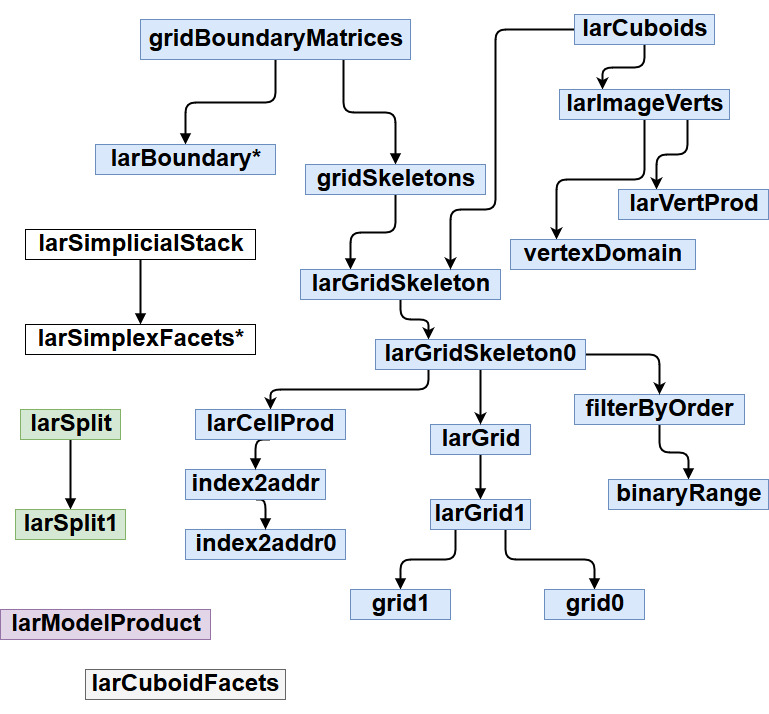
\includegraphics[scale=0.4]{grafo.jpg}
\caption{Graph of recall-functions}
\label{fig:grafo}
\end{figure}

\subsection{Module functions}

LIST OF FUNCTIONS:

\begin{itemize}
\item larSplit
\item grid0 
\item grid1
\item larGrid
\item larVertProd
\item index2addr
\item larCellProd
\item binaryRange
\item filterByOrder
\item larGridSkeleton
\item larCuboids
\item gridSkeletons
\item gridBoundaryMatrices
\item larModelProduct
\end{itemize}
\begin{center}
\begin{tabular}{ccc}
\\
\hline
{EXTERNAL FUNCTIONS}& API& LOCAL\\
\hline
larBoundary& larSplit& larSplit1\\
\hline
larSimplexFacets& larGrid& larGrid1\\
\hline
{Standard pyplasm functions}& larCuboidFacets& larGridSkeleton0\\
\hline
{Standard python functions}& larSimplicialStack& vertexDomain\\
\hline
& larGridSkeleton& index2addr0\\
\hline
& larModelProduct& grid0\\
\hline
& larCuboids& grid1\\
\hline
& gridSkeletons& binaryRange\\
\hline
& & filterByOrder\\
\hline
& &	larVertProd\\
\hline
& & index2addr\\
\hline
& &	larCellProd\\
\hline
& &	larImageVerts\\
\hline
& & gridBoundaryMatrices\\
\hline
\\
\end{tabular}\\
\end{center}
\subsection{API functions}

\emph{larSplit}: The second order larSplit function is used to subdivide the real interval $[0, dom]$ into n equal parts. It returns the list of $n + 1$ vertices 1D of this decomposition.
\\ \\
\emph{larGrid}:  This function generate the LAR representation of the cells of either a $0-$ or a $1-dimensional$ complex, depending on the value of the $d$ parameter, to take values in the set ${0, 1}$, and providing the order of the output complex.
\\ \\
\emph{larGridSkeleton}: It can generate the various subsets of cells of a $d$-dimensional cuboidal grid skeleton.
It’s usefull to assemble the components of a skeleton of a grid. It returns the list of indices of vertices, edges or faces (it depends form the dimension given in input).
\\ \\
\emph{larCuboids}: It constructs (iper-)cuboidal grids. The generated complex is a solid, and we can include cells of every dimension. It returns a tupla of vertices and faces. 
\\ \\
\emph{gridSkeletons}: It returns a list of cellular k-complexes ($0 \leq k \leq d$) with dimension $d$, where $d = len(shape)$, in the macro below, where the input is given by the shape of the grid, i.e. by the list of cell items in each coordinate direction.
\\ \\
\emph{larModelProduct}: A LAR model is a pair (geometry, topology), where geometry is the list of vertices and topology is the list of cells, in some dimension $d$. This function takes in input a pair of LAR model and returns the LAR model of their Cartesian product.
\\ \\
\emph{larSimplicialStack}: The whole stack of LAR cell-vertex arrays is returned ordered from $0$-cells to $d$-cells.
It’s usefull for the calculus of simplices. 
\\ \\
\emph{larCuboidsFacets}: It extracts facets from cuboidal complexes. It returns a tupla of vertices and facets.

%-------------------------------------------------------------------------------

\section{Scripts}
\paragraph{Translation\\}
Special attention is given to \emph{translation}. Main difference between Python and Julia language is the indexing of array. Python uses 0-based indexing, Julia uses 1-based indexing. It also changes the type of some methods because another difference between Python and Julia library is the type of vertices: in Python code, vertices are array in array; in Julia code, vertices are represented as two-dimensional array, matrix.
\paragraph{Improvement of functions\\}
About the \emph{improvement} of the code, in technical-computing languages, it is common to have  \emph{vectorized} versions of functions, which simply apply a given function $f(x)$ to each element of an array $A$ to yield a new array via $f(A)$. In general, vectorized code replaces the loop for moving through a vector one component at a time. In Julia, function $f$ can be applied elementwise to any array (or other collection) with the syntax $f.(A)$.

For some functions it also was possible to \emph{parallelize} the code.
Parallel computing is a type of computation in which many calculations or the execution of processes are carried out concurrently. Large problems can often be divided into smaller ones, which can then be solved at the same time.
\paragraph{Test\\}
The \texttt{Base.Test} module provides simple unit testing functionality. Unit testing is a way to see if code is correct by checking that the results are what you expect. It can be helpful to ensure you code still works after you make changes, and can be used when developing as a way of specifying the behaviors your code should have when complete.\citep{julia}
 
\begin{flushleft}\small
\begin{list}{}{}\item
\begin{Verbatim}[tabsize=4]
using Base.Test
\end{Verbatim}
\end{list}
\end{flushleft}

\paragraph{Execution times\\}
Parallel computing is performed on 4 processes in our computer. 

\begin{flushleft}\small
\begin{list}{}{} \item
   \begin{Verbatim}[tabsize=4]
n=4
addprocs(n)

using Plots

N=10
   \end{Verbatim}
\end{list}
\end{flushleft}
\vspace{2ex}
For studying \texttt{execution times} for each function we create this function \texttt{Time}.
This function takes as input an integer value (the number of loops), function and its arguments, returns an array of all the execution times for each loop. 
We use the macro $@elapsed$ to computing the execution time than the macro $@time$ that returns allocation memory too.  
Since at the first call of $@elapsed$ $f(args)$, $f$ must be compiled, the first time we do not consider it, because it will certainly be longer than normal.

\begin{list}{}{} \item
   \begin{Verbatim}[tabsize=4]
function Time(N::Int,f::Function,args)
	timings = Array{Float64}(N)
	@elapsed f(args)
	for i in 1:N
		timings[i] = @elapsed f(args)
	end
	return timings
end
   \end{Verbatim}
\end{list}
\vspace{2ex}
For each function we compute the time with different input and we study mean and standard error $ e=\frac{std}{\sqrt{N}}$ with Julia methods \texttt{mean()} and \texttt{std()}.
\\
\\
So there are two possibilities.

For large N the time values for each individual input are more precise, since the computer calculates the times with an error. But having to do a lot of loops it is not possible to study for very large inputs, it will take too much time.

For small N it is possible to increase the maximum input passed to the function and to study with less precision larger inputs.
This study was done with $N = 10$ and changing the inputs if necessary.
\vspace{2ex}

\\ \\
NOTE: for vectorized version, it has been inserted a prefix \texttt{v} ; for parallelized version, a prefix \texttt{p}.
\\ \\
To use all these functions, you have to import these packages:
\begin{flushleft}\small
\begin{list}{}{} \item
\begin{Verbatim}
using IterTools
using DataStructures
using Combinatorics
\end{Verbatim}
\end{list}
\end{flushleft}
\vspace{1ex}
To use these functions on all processes, you have to use:
\begin{flushleft}\small
\begin{list}{}{} \item
\begin{Verbatim}
@everywhere using IterTools
@everywhere using DataStructures
@everywhere using Combinatorics
\end{Verbatim}
\end{list}
\end{flushleft}


%-----------------------------------------------------------------

\subsection{larSplit:}

\subsubsection{Translation}

\begin{flushleft} \small
\begin{center}
\begin{tabular}{|p{16cm}|}
\hline
\cellcolor[gray]{.9}Python\\
\hline
\end{tabular}
\end{center}

\begin{list}{}{} \item
\begin{Verbatim}[tabsize=3]
def larSplit(dom):
    def larSplit1(n):
        # assert n > 0 and isinstance(n,int)
        item = float(dom)/n
        ints = range(n+1)
        items = [item]*(n+1)
        vertices = [[int*item]
                for (int,item) in zip(ints,items)]
        return vertices
    return larSplit1
\end{Verbatim}
\end{list}

\begin{center}
\begin{tabular}{|p{16cm}|}
\hline
\cellcolor[gray]{.9}Julia\\
\hline
\end{tabular}
\end{center}

\begin{list}{}{} \item
\begin{Verbatim}[tabsize=4]
function larSplit(dom)
    function larSplit1(n)
        item = dom/n
        ints = range(0,n+1) 
        vertices=[ints*item;]
        return reshape(vertices,1,n+1)
    end
    return larSplit1
end
\end{Verbatim}
\end{list}
\end{flushleft}
\vspace{2ex}
This is a second order function, that is, it is applied to two arguments: the first argument is length of the interval as \texttt{float}, the second is the number of intervals as \texttt{int}. Python output is the list of $n + 1$ vertices $1D$, each represented as a singleton list. Julia output is list of $n + 1$ vertices $1D$, as bidimensional Array.

\subsubsection{Test}
\begin{center}
\begin{tabular}{|p{16cm}|}
\hline
\cellcolor[gray]{.9}Test\\
\hline
\end{tabular}
\end{center}

\begin{flushleft}\small
\begin{list}{}{} \item
\begin{Verbatim}[tabsize=4]
@testset "larSplit Tests" begin
       quarto=larSplit(5)(4)[5]-larSplit(5)(4)[4]
       terzo=larSplit(5)(4)[4]-larSplit(5)(4)[3]
       secondo=larSplit(5)(4)[3]-larSplit(5)(4)[2]
       primo=larSplit(5)(4)[2]-larSplit(5)(4)[1]    
           @test primo == 1.25
           @test secondo == 1.25
           @test terzo == 1.25
           @test quarto == 1.25
end
\end{Verbatim}
\end{list}
\end{flushleft}
%-------------------------------------------------------------------------------

\subsection{larGrid:}

\begin{flushleft} \small
\subsubsection{Translation}
\vspace{1ex}
\begin{center}
\begin{tabular}{|p{16cm}|}
\hline
\cellcolor[gray]{.9}Python\\
\hline
\end{tabular}
\end{center}
\begin{list}{}{} \item
\begin{Verbatim}[tabsize=4]
def grid0(n):
    cells = AA(LIST)(range(n+1))
    return cells

def grid1(n):
    ints = range(n+1)
    cells = TRANS([ints[:-1],ints[1:]])
    return cells

def larGrid(n):
    def larGrid1(d):
        if d==0: return grid0(n)
        elif d==1: return grid1(n)
    return larGrid1
\end{Verbatim}
\end{list}

\begin{center}
\begin{tabular}{|p{16cm}|}
\hline
\cellcolor[gray]{.9}Julia\\
\hline
\end{tabular}
\end{center}

\begin{list}{}{} \item
\begin{Verbatim}[tabsize=4]
function grid_0(n)
    return hcat([range(0,n+1);]...)
end

function grid_1(n)
    return hcat([[i,i+1] for i in range(0,n)]...)
end

function larGrid(n)
    function larGrid1(d)
        if d==0 
            return grid_0(n)
        elseif d==1 
            return grid_1(n) 
        end
    end
    return larGrid1
end
\end{Verbatim}
\end{list}
\end{flushleft}
\vspace{2ex}
This function is usefull to generate uniform $0D$ and $1D$ cellular complex, with $n$ cells.
In translated code standard methods of Python, like \texttt{AA()()} ( = ApplyToAll ) and \texttt{TRANS()} ( = Transpose ), are replaced by Julia method \texttt{hcat()}, that concatenate along dimension 2.
\vspace{2ex}
\subsubsection{Parallel computing}
\vspace{1ex}
This version shouldn't be taken into account.

In Section "Execution time", we are going to prove with an example, comparing execution times, that this type of parallelization does not work. Indeed the execution time is higher then serial version, due to the fact that it takes time to distribute the "fake" work on all the processes, because the workers do not have a real work to do.
\begin{flushleft} \small
\begin{center}
\begin{tabular}{|p{16cm}|}
\hline
\cellcolor[gray]{.9}Parallel\\
\hline
\end{tabular}
\end{center}
\vspace{2ex}
\begin{list}{}{} \item
\begin{Verbatim}[tabsize=4]
@everywhere function pgrid_0(n)
	W=@parallel (hcat) for i in range(0,n+1) 
		[i] 
	end
	return W
end

@everywhere function pgrid_1(n)
	W=@parallel (hcat) for i in range(0,n) 
		[i,i+1] 
	end
	return W
end

@everywhere function plarGrid(n)
    function larGrid1(d)
        if d==0 
            return pgrid_0(n)
        elseif d==1 
            return pgrid_1(n) 
        end
    end
    return larGrid1
end
\end{Verbatim}
\end{list}
\vspace{2ex}
\footnotesize\addtolength{\baselineskip}{-1ex}
\end{flushleft}
Macro \texttt{@everywhere expr} execute an expression under Main everywhere, on all processes. The construct, \texttt{@parallel (reduction) for}, implements the pattern of assigning iterations to multiple processes, and combining them with a specified reduction (in this case (\texttt{hcat})). 
\vspace{2ex}

\subsubsection{Test}
\begin{center}
\begin{tabular}{|p{16cm}|}
\hline
\cellcolor[gray]{.9}Test\\
\hline
\end{tabular}
\end{center}

\begin{flushleft}\small
\begin{list}{}{} \item
\begin{Verbatim}[tabsize=4]
@testset "larGrid Tests" begin
	@testset "grid_0" begin
			@test grid_0(1) == [0  1]
			@test grid_0(2) == [0  1  2]
			@test grid_0(3) == [0  1  2  3]
	end
   
	@testset "grid_1 Tests" begin
			@test repr(grid_1(1)) == "[0; 1]"
			@test grid_1(2) == [0 1; 1 2]
			@test grid_1(3) == [0 1 2; 1 2 3]
	end
   
	@testset "larGrid" begin
			@test repr(larGrid(1)(0)) == "[0 1]"
			@test repr(larGrid(1)(1)) == "[0; 1]"
			@test larGrid(2)(0) == [0  1  2]
			@test larGrid(2)(1) == [0 1; 1 2]
	end
end 

@testset "plarGrid Tests" begin
   		@testset "pgrid_0" begin
    			@test pgrid_0(1) == [0  1]
    			@test pgrid_0(2) == [0  1  2]
    			@test pgrid_0(3) == [0  1  2  3]
		end
       
		@testset "pgrid_1 Tests" begin
      			@test repr(pgrid_1(1)) == "[0, 1]"
    			@test pgrid_1(2) == [0 1; 1 2]
    			@test pgrid_1(3) == [0 1 2; 1 2 3]
		end
   
   		@testset "plarGrid" begin
    			@test repr(plarGrid(1)(0)) == "[0 1]"
    			@test repr(plarGrid(1)(1)) == "[0, 1]"
    			@test plarGrid(2)(0) == [0  1  2]
    			@test plarGrid(2)(1) == [0 1; 1 2]
    			@test plarGrid(3)(0) == [0  1  2  3]
    			@test plarGrid(3)(1) == [0  1  2; 1  2  3]
		end
end 
\end{Verbatim}
\end{list}
\end{flushleft}
\subsubsection{Execution time}
\begin{center}
\begin{tabular}{|p{16cm}|}
\hline
\cellcolor[gray]{.9}Execution time\\
\hline
\end{tabular}
\end{center}
Let us now prove what we have mentioned before in the parallelization of the larGrid function.
In this example it is clear that the parallelized loop works very well, because the workers have a job to do.
\begin{flushleft}\small
\begin{list}{}{} \item
   \begin{Verbatim}[tabsize=4]
Input: s=0; @elapsed for i in 1:200000000
       s=s+Int(rand(Bool))
       end
Output: 23.247962902

Input: @elapsed nheads = @parallel (+) for i = 1:200000000
           Int(rand(Bool))
       end
Output: 1.744299978
\end{Verbatim}
\end{list}
\end{flushleft}
Comparing the times of the serial version with parallel version of larGrid function, it is easy to notice that the parallelization does not work.
\vspace{2ex}
\paragraph{Serial}
\begin{flushleft}\small
\begin{list}{}{} \item
    \begin{Verbatim}[tabsize=4]
datas=[Time(N,larGrid(j),(1)) for j in [10^2,5*10^2,10^3,5*10^3,10^4,5*10^4,10^5]]

xs=[1:length(datas);]
ys=mean.(datas)
yerrs=std.(datas)/sqrt(N)

plot(xs,ys,yaxis="Time (s)",xlims = (0,length(datas)+1), yerr = yerrs,
                        xaxis="Input", title="larGrid",label=["Serial"],lw=1)
    \end{Verbatim}
\end{list}
\end{flushleft} 

\paragraph{Parallel}
\begin{flushleft}\small
\begin{list}{}{} \item
    \begin{Verbatim}[tabsize=4]
datap=[Time(N,plarGrid(j),(1)) for j in [10^2,5*10^2,10^3,5*10^3,10^4,5*10^4,10^5]]

xp=[1:length(datap);]
yp=mean.(datap)
yerrp=std.(datap)/sqrt(N)

plot(xp,yp,yaxis="Time (s)",xlims = (0,length(datap)+1), yerr = yerrp,
                    xaxis="Input", title="larGrid",label=["Parallel"],lw=1)
    \end{Verbatim}
\end{list}
\end{flushleft}  

\begin{figure}[h!]
\centering
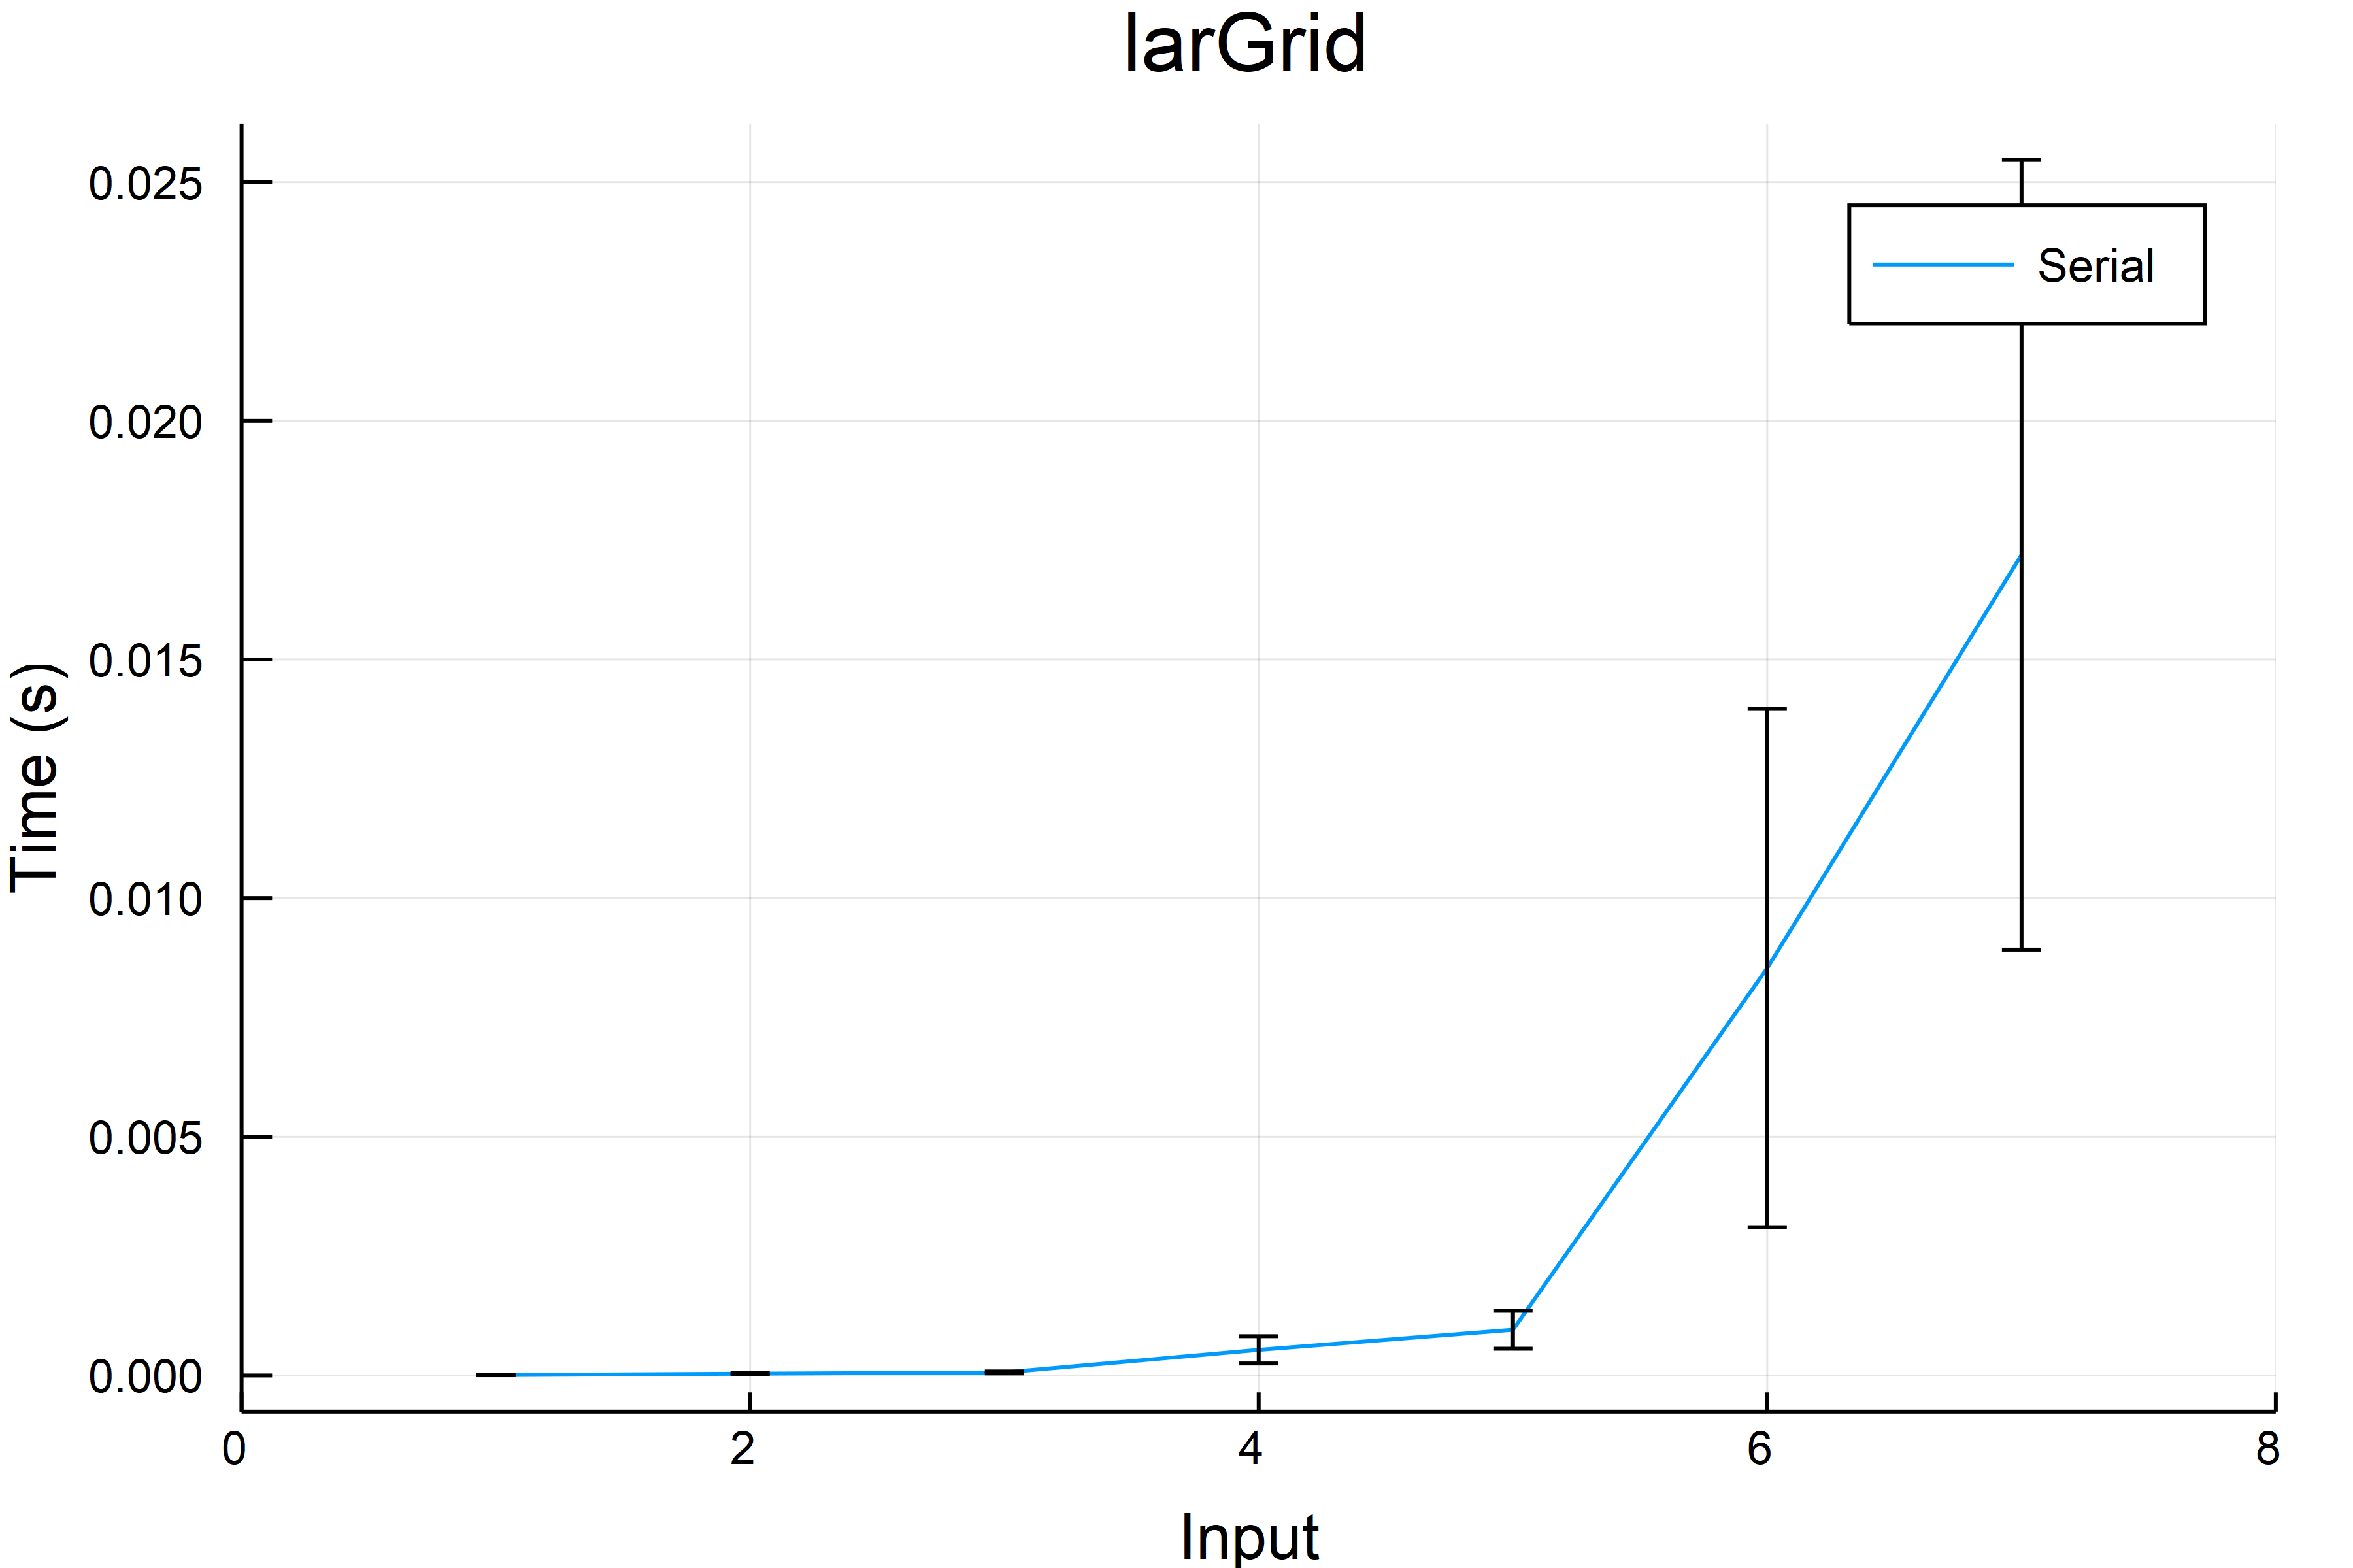
\includegraphics[scale=0.06]{larGridSer.png}
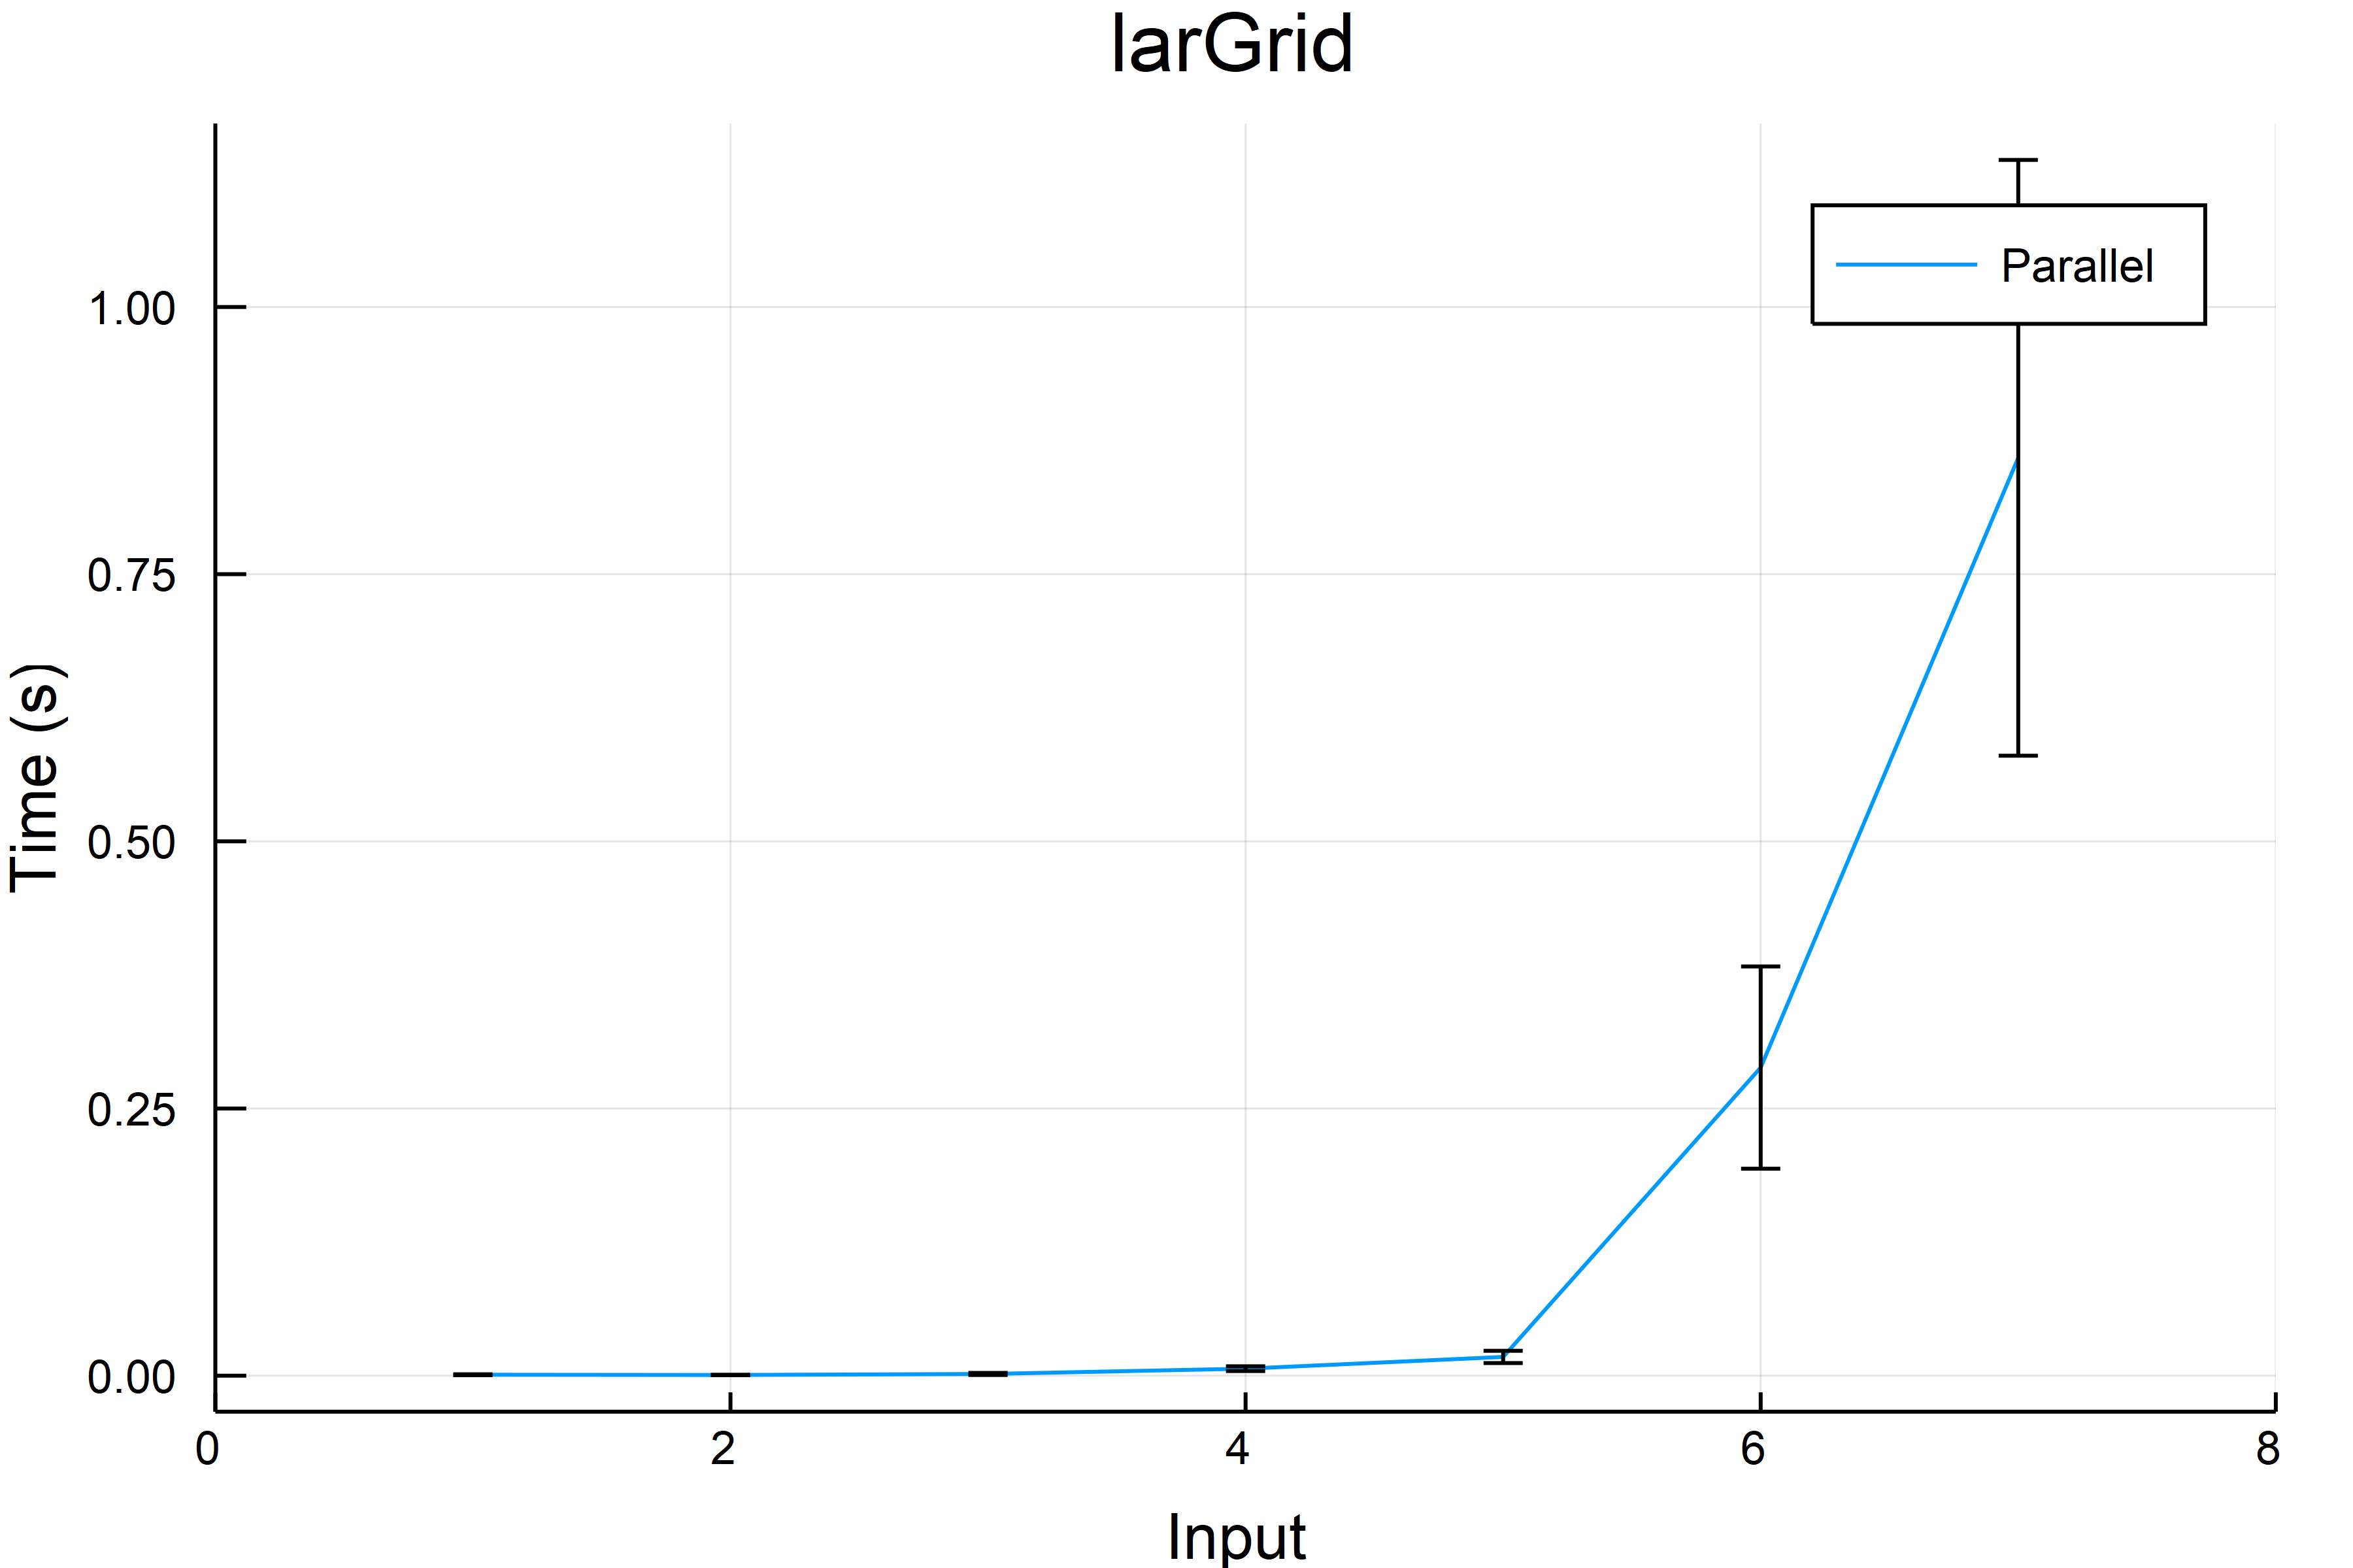
\includegraphics[scale=0.06]{larGridPar.png}
\end{figure}

\paragraph{Compare}
\begin{flushleft}\small
\begin{list}{}{} \item
    \begin{Verbatim}[tabsize=4]
x=[xs,xp]
y=[ys,yp]

plot(x,y,yaxis="Time (s)",xlims = (0,length(datap)+1), xaxis="Input",
                            title="larGrid",label=["Serial" "Parallel"],lw=1)
    \end{Verbatim}
\end{list}
\end{flushleft}   
\vspace{3ex}
\begin{figure}[h!]
\centering
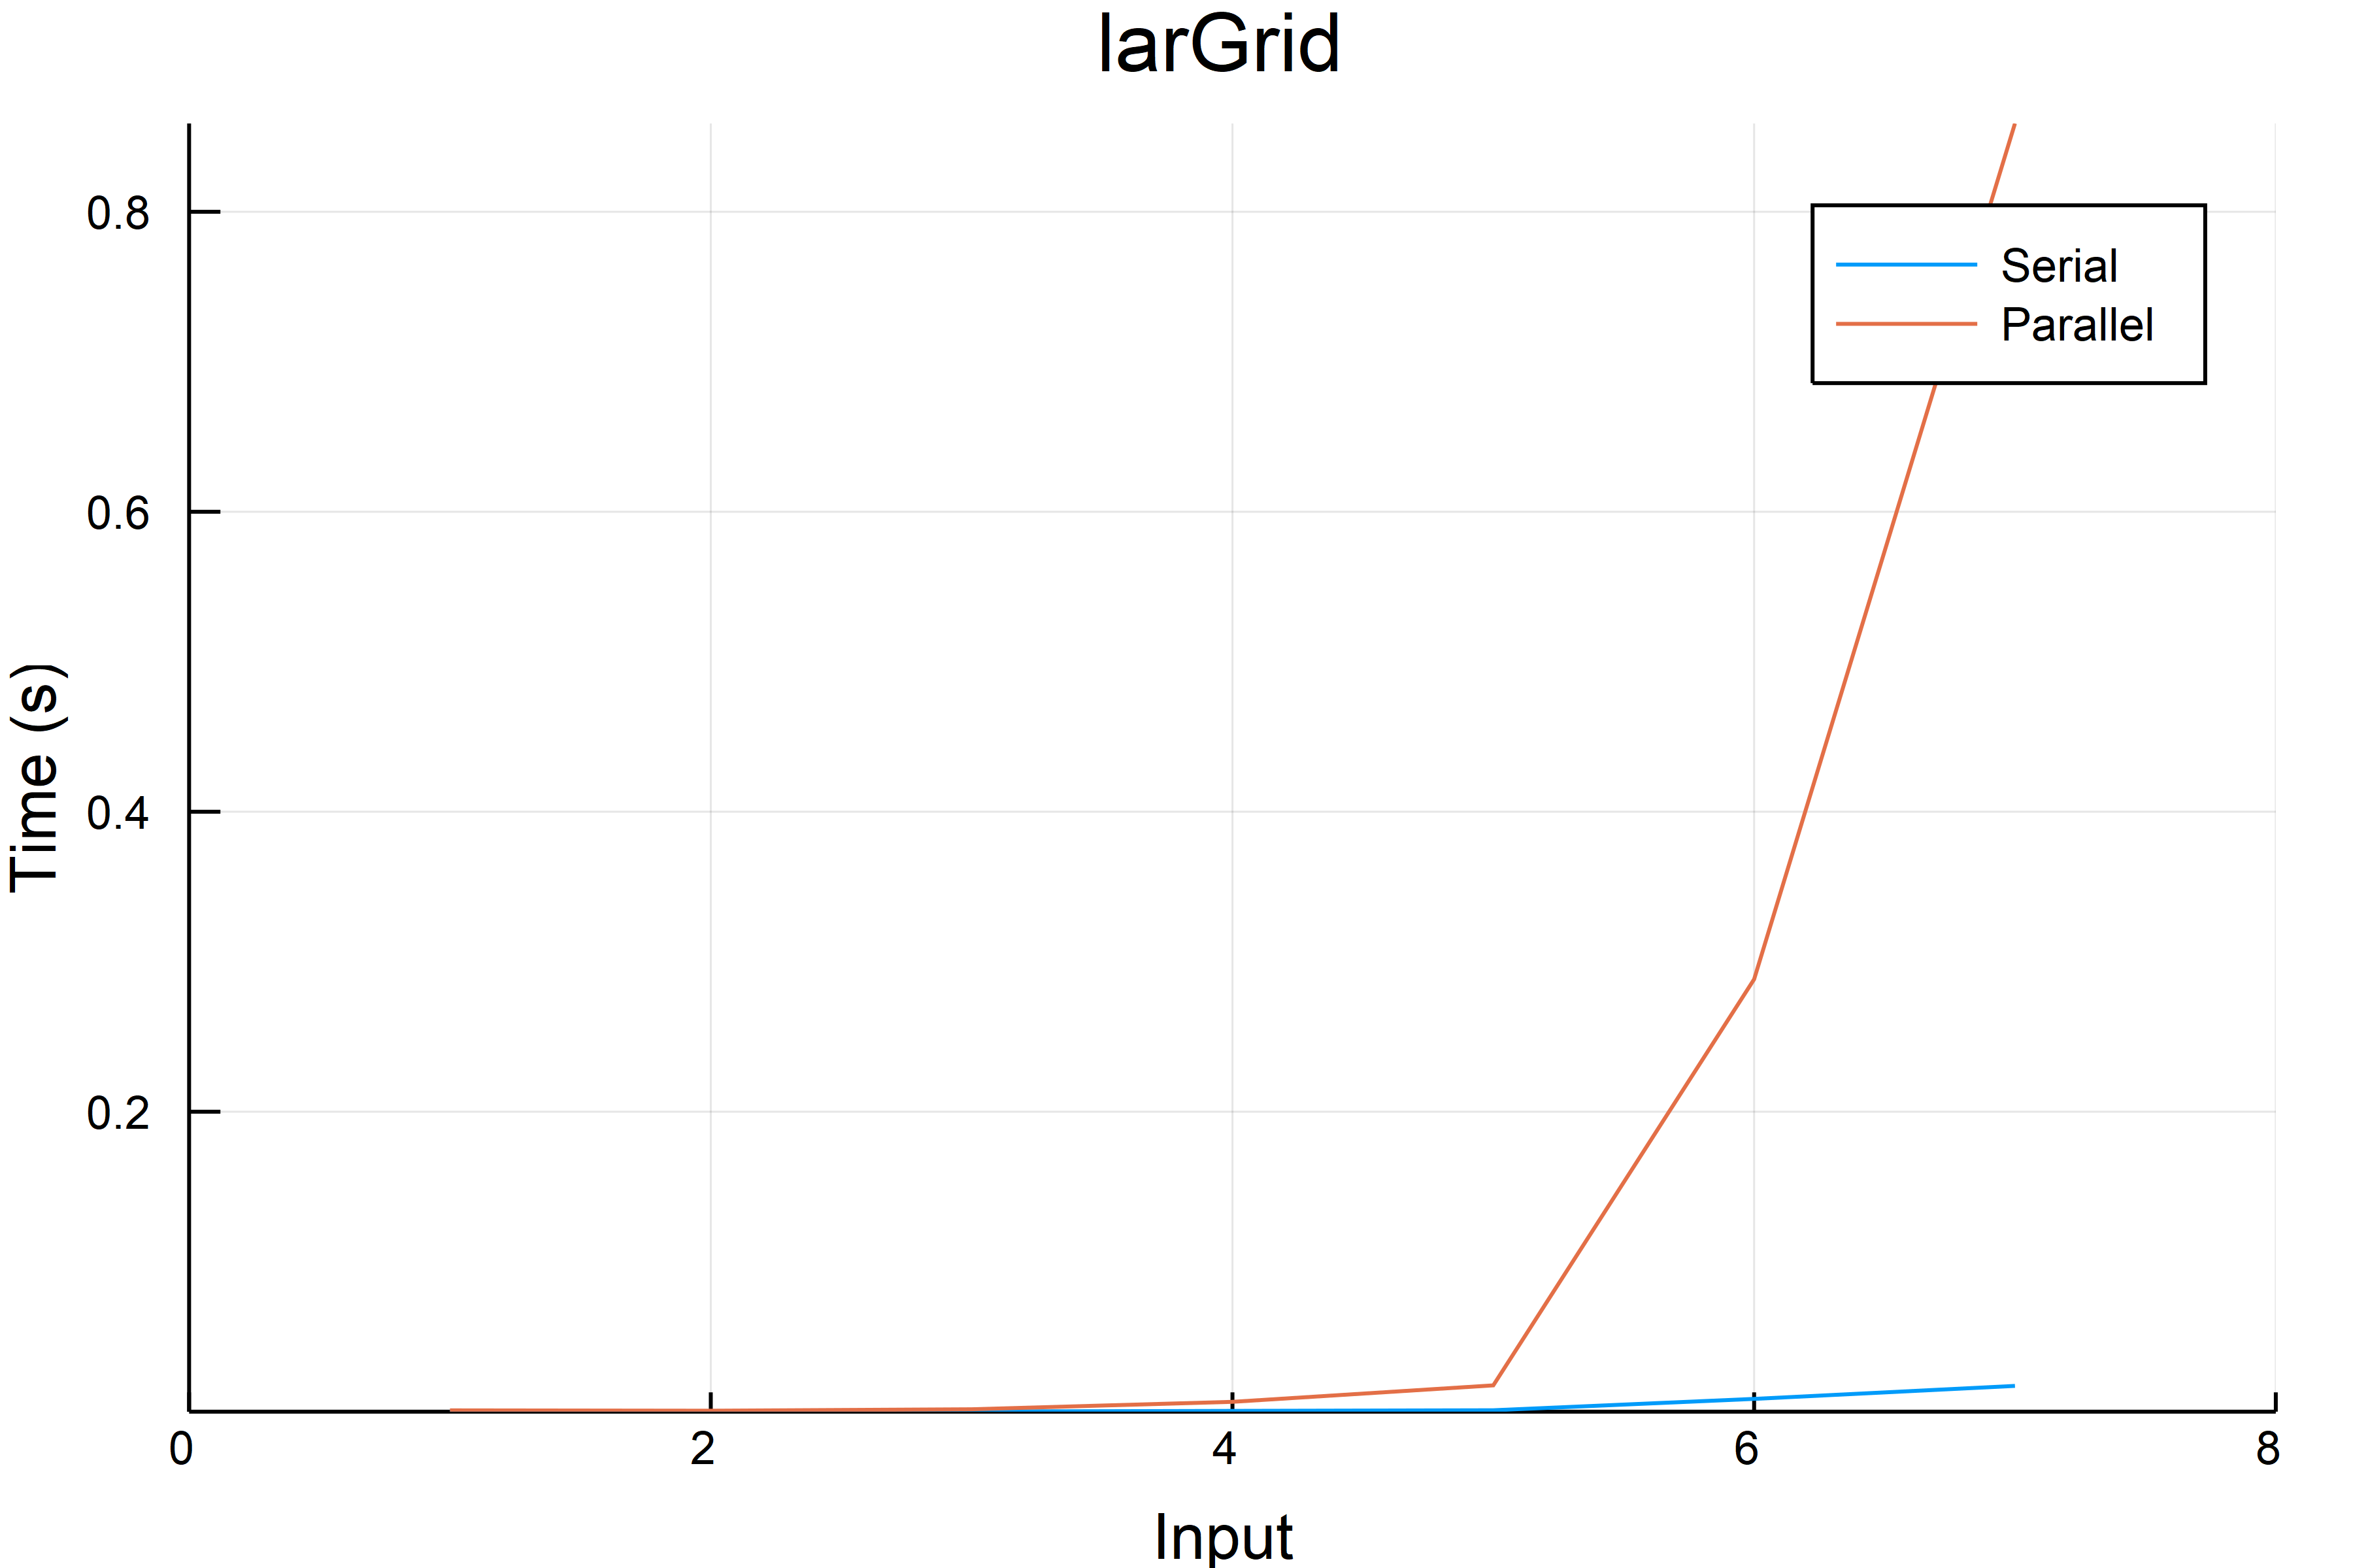
\includegraphics[scale=0.06]{larGridCom.png}
\end{figure}

\vspace{4ex}

%-------------------------------------------------------------------------------
\subsection{larCuboidsFacets:}

\begin{flushleft} \small
\subsubsection{Translation}
\vspace{1ex}
\begin{center}
\begin{tabular}{|p{16cm}|}
\hline
\cellcolor[gray]{.9}Python\\
\hline
\end{tabular}
\end{center}
\vspace{2ex}
\begin{list}{}{} \item
\begin{Verbatim}[tabsize=3]
def larCuboidsFacets((V,cells)):
	dim = len(V[0])
	n = int(2**(dim-1))
	facets = []
	for cell in cells:
		coords = [AR([V[v],v]) for v in cell] 
		doubleFacets = [sorted(coords,
		  key=(lambda x: x[k])) for k in range(dim)] 
		facets += AA(AA(LAST))(CAT([[pair[:n],pair[n:]] for pair in doubleFacets]))
	facets = AA(eval)(set(AA(str)(facets))) 
	return V,sorted(facets)
\end{Verbatim}
\end{list}
\vspace{2ex}
\begin{center}
\begin{tabular}{|p{16cm}|}
\hline
\cellcolor[gray]{.9}Julia\\
\hline
\end{tabular}
\end{center}
\vspace{2ex}
\begin{list}{}{} \item
\begin{Verbatim}[tabsize=3]
function larCuboidsFacets(V,cells)
   dim = size(V,1)
   n = 2^(dim-1)
   facets = Array{Int64,1}[]
   for cell in cells
      Vert=hcat([V[:,i] for i in cell]...)
      coords = vcat(Vert,reshape(cell,(1,size(cell)[1])))
      doubleFacets=hcat([coords[:,sortperm(coords[k,:])] for k in range(1,dim)]...)
      lastRow=doubleFacets[dim+1,:]
      facets0 = reshape(lastRow,(n,Int(size(lastRow)[1]/n)))
      append!(facets,collect([facets0[:,i] for i in range(1,size(facets0)[2])]))
   end
   facets = unique(facets)
   return V,sort(facets, by = x -> x[1])
end

function larCuboidsFacets(model)
    V,cells=model
    larCuboidsFacets(V,cells)
end
  \end{Verbatim}
\end{list}

\end{flushleft}
\vspace{2ex}
The algorithm of this function is the same during translation, but there is a little difference in order to add the elements of a collection to the end of another collection. In Python language can be used a simple \texttt{"+"}, in Julia language is used \texttt{append!()}. 

To sort $coords$ in $doubleFacets$, in Julia, can be used \texttt{sortperm}, a function that returns a permutation vector of indices of your vector, in according to choosing algorithm for a particular sorting.
\vspace{2ex}

\subsubsection{Vectorize}
\vspace{1ex}
To vectorize this function on array named $cells$, loop was removed and a new intermediate \texttt{vlarCuboidsFacets0} function was constructed.
\begin{flushleft} \small
\begin{center}
\begin{tabular}{|p{16cm}|}
\hline
\cellcolor[gray]{.9}Vectorized code\\
\hline
\end{tabular}
\end{center}
\vspace{2ex}
\begin{list}{}{} \item
   \begin{Verbatim}[tabsize=4]
function vlarCuboidsFacets0(n,dim,V)
	function vlarCuboidsFacets1(cell)
		facets=Array{Int64,1}[]
		Vert=hcat([V[:,i] for i in cell]...)
		coords = vcat(Vert,reshape(cell,(1,size(cell)[1])))
		doubleFacets=hcat([coords[:,sortperm(coords[k,:])] for k in range(1,dim)]...)
		lastRow=doubleFacets[dim+1,:]
		facets0 = reshape(lastRow,(n,Int(size(lastRow)[1]/n)))
		append!(facets,collect([facets0[:,i] for i in range(1,size(facets0)[2])]))
		return(facets)
	end
	return vlarCuboidsFacets1
end

function vlarCuboidsFacets(V,cells)
	dim = size(V,1)
	n = 2^(dim-1)
	W=vlarCuboidsFacets0(n,dim,V).(cells)
	WW=union([W[i] for i in range(1,length(W))]...)
	facets = unique(WW)
	return V,sort(facets, by = x -> x[1])
end

function vlarCuboidsFacets(model)
    V,cells=model
    vlarCuboidsFacets(V,cells)
end
   \end{Verbatim}
\end{list}
\end{flushleft}

\vspace{2ex}
\subsubsection{Parallel computing}
\vspace{1ex}
It can be parallelized in two ways, using the construct \texttt{@parallel (reduction) for} or using the Julia standard method \texttt{pmap(f,args)}.
In Section "Execution time" we are going to determine which constructs is best.
Julia's \texttt{pmap()} is designed for the case where each function call does a large amount of work. Only worker processes are used by both  \texttt{pmap()} and \texttt{@parallel (reduction) for} for the parallel computation. In case of \texttt{@parallel (reduction) for}, the final reduction is done on the calling process.
\vspace{2ex}
\begin{flushleft} \small
\begin{center}
\begin{tabular}{|p{16cm}|}
\hline
\cellcolor[gray]{.9}Parallel Loop\\
\hline
\end{tabular}
\end{center}
\vspace{2ex}
\begin{list}{}{} \item
   \begin{Verbatim}[tabsize=4]
@everywhere function plarCuboidsFacets0(n,dim,V,cell,facets)
	Vert=@parallel (hcat) for i in cell V[:,i] end
	coords = vcat(Vert,reshape(cell,(1,size(cell)[1])))
	doubleFacets=@parallel (hcat) for k in range(1,dim)
		coords[:,sortperm(coords[k,:])] 
	end
	lastRow=doubleFacets[dim+1,:]
	facets0 = reshape(lastRow,(n,Int(size(lastRow)[1]/n)))
	append!(facets,collect([facets0[:,i] for i in range(1,size(facets0)[2])]))
	return facets
end

function plarCuboidsFacets(V,cells)
	dim = size(V,1)
	n = 2^(dim-1)
	facets = []
	W=@parallel (append!) for cell in cells
			fetch( @spawn plarCuboidsFacets0(n,dim,V,cell,facets))
	end
	facets = unique(W)
	return V,sort(facets, by = x -> x[1])
end

function plarCuboidsFacets(model)
    V,cells=model
    plarCuboidsFacets(V,cells)
end
   \end{Verbatim}
\end{list}
\vspace{2ex}


\begin{center}
\begin{tabular}{|p{16cm}|}
\hline
\cellcolor[gray]{.9}Parallel Map\\
\hline
\end{tabular}
\end{center}
\vspace{2ex}

\begin{list}{}{} \item
   \begin{Verbatim}[tabsize=4]
@everywhere function pmlarCuboidsFacets0(n,dim,V,facets)
	function pmlarCuboidsFacets1(cell)
		Vert = @parallel (hcat) for i in cell V[:,i] end
		coords = vcat(Vert,reshape(cell,(1,size(cell)[1])))
		doubleFacets = @parallel (hcat) for k in range(1,dim) 
		    coords[:,sortperm(coords[k,:])] 
		end
		lastRow = doubleFacets[dim+1,:]
		facets0 = reshape(lastRow,(n,Int(size(lastRow)[1]/n)))
		append!(facets,collect([facets0[:,i] for i in range(1,size(facets0)[2])]))
		return facets
	end
	return pmlarCuboidsFacets1
end

function pmlarCuboidsFacets(V,cells)
	dim = size(V,1)
	n = 2^(dim-1)
	facets = []
	W = pmap(pmlarCuboidsFacets0(n,dim,V,facets),cells)
	WW = @parallel (union) for i in range(1,length(W)) W[i] end
	facets = unique(WW)
	return V,sort(facets, by = x -> x[1])
end

function pmlarCuboidsFacets(model)
    V,cells=model
    pmlarCuboidsFacets(V,cells)
end
   \end{Verbatim}
\end{list}
\end{flushleft}
\subsubsection{Test}
\begin{center}
\begin{tabular}{|p{16cm}|}
\hline
\cellcolor[gray]{.9}Test\\
\hline
\end{tabular}
\end{center}

\begin{flushleft}\small
\begin{list}{}{} \item
    \begin{Verbatim}[tabsize=4]
@testset "larCuboidsFacets Tests" begin
		@test length(larCuboidsFacets([[0,0] [0,1] [1,1] [1,0]], [[1,2,3,4]])[2]) == 4
		@test size(larCuboidsFacets([[0,0] [0,1] [1,1] [1,0]], [[1,2,3,4]])[1],2) == 4 
end
	
@testset "vlarCuboidsFacets Tests" begin
		    @test length(vlarCuboidsFacets([[0,0] [0,1] [1,1] [1,0]], [[1,2,3,4]])[2]) == 4
		    @test size(vlarCuboidsFacets([[0,0] [0,1] [1,1] [1,0]], [[1,2,3,4]])[1],2) == 4 
end

@testset "plarCuboidsFacets Tests" begin
		    @test length(plarCuboidsFacets([[0,0] [0,1] [1,1] [1,0]], [[1,2,3,4]])[2]) == 4
    		@test size(plarCuboidsFacets([[0,0] [0,1] [1,1] [1,0]], [[1,2,3,4]])[1],2) == 4 
    	end
	
@testset "pmlarCuboidsFacets Tests" begin
    		@test length(pmlarCuboidsFacets([[0,0] [0,1] [1,1] [1,0]], [[1,2,3,4]])[2]) == 4
    		@test size(pmlarCuboidsFacets([[0,0] [0,1] [1,1] [1,0]], [[1,2,3,4]])[1],2) == 4 
end
   \end{Verbatim}
\end{list}
\end{flushleft}
\subsubsection{Execution time}
\begin{center}
\begin{tabular}{|p{16cm}|}
\hline
\cellcolor[gray]{.9}Execution time\\
\hline
\end{tabular}
\end{center}

\paragraph{Serial}
\begin{flushleft}\small
\begin{list}{}{} \item
    \begin{Verbatim}[tabsize=4]
input=[larCuboids([n,n,n]) for n in [1:20;]]

datas=[Time(N,larCuboidsFacets,(j)) for j in input]

xs=[1:length(datas);]
ys=mean.(datas)
yerrs=std.(datas)/sqrt(N)

plot(xs,ys,yaxis="Time (s)",xlims = (0,length(datas)+1), yerr = yerrs, xaxis="Input",
                                            title="larCuboidsFacets",label=["Serial"],lw=1)
    \end{Verbatim}
\end{list}
\end{flushleft}  

\paragraph{Vectorize}
\begin{flushleft}\small
\begin{list}{}{} \item
    \begin{Verbatim}[tabsize=4]
datav=[Time(N,vlarCuboidsFacets,j) for j in input]

xv=[1:length(datav);]
yv=mean.(datav)
yerrv=std.(datav)/sqrt(N)

plot(xv,yv,yaxis="Time (s)",xlims = (0,length(datav)+1), yerr = yerrv, xaxis="Input",   
                                        title="larCuboidsFacets",label=["Vectorize"],lw=1)
    \end{Verbatim}
\end{list}
\end{flushleft}

\begin{figure}[h!]
\centering
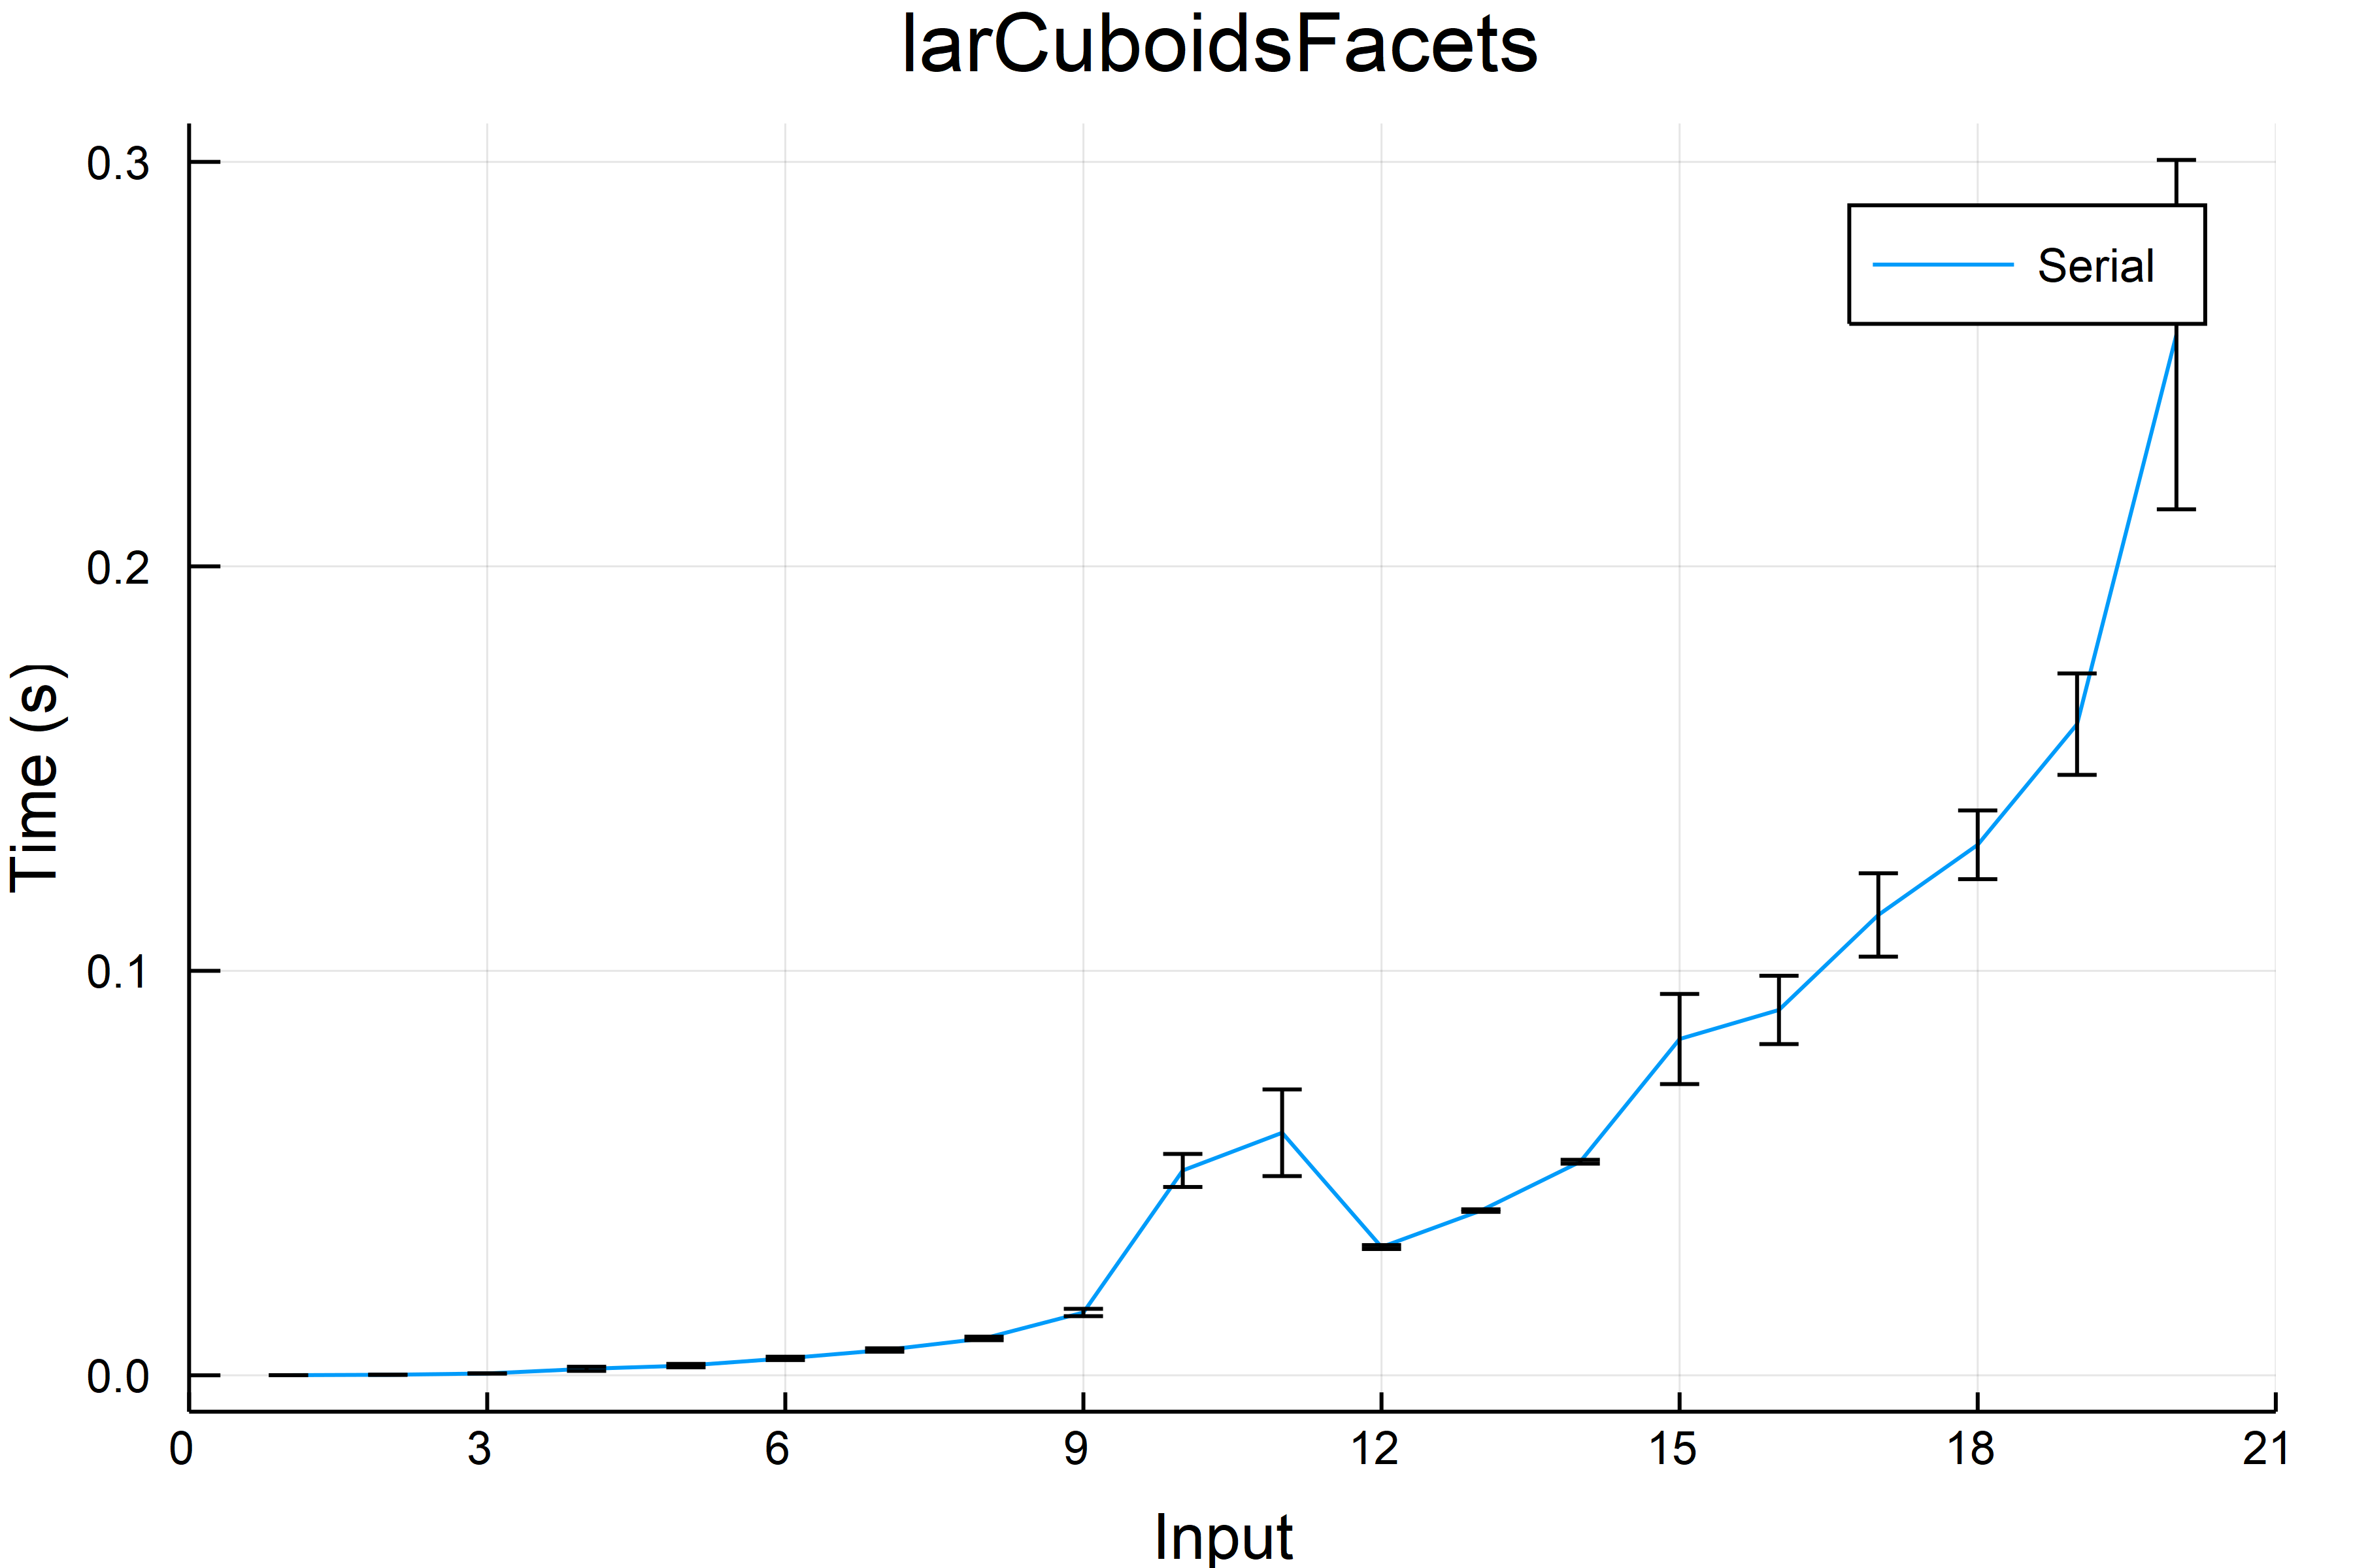
\includegraphics[scale=0.06]{larCuboidsFacetsSer.png}
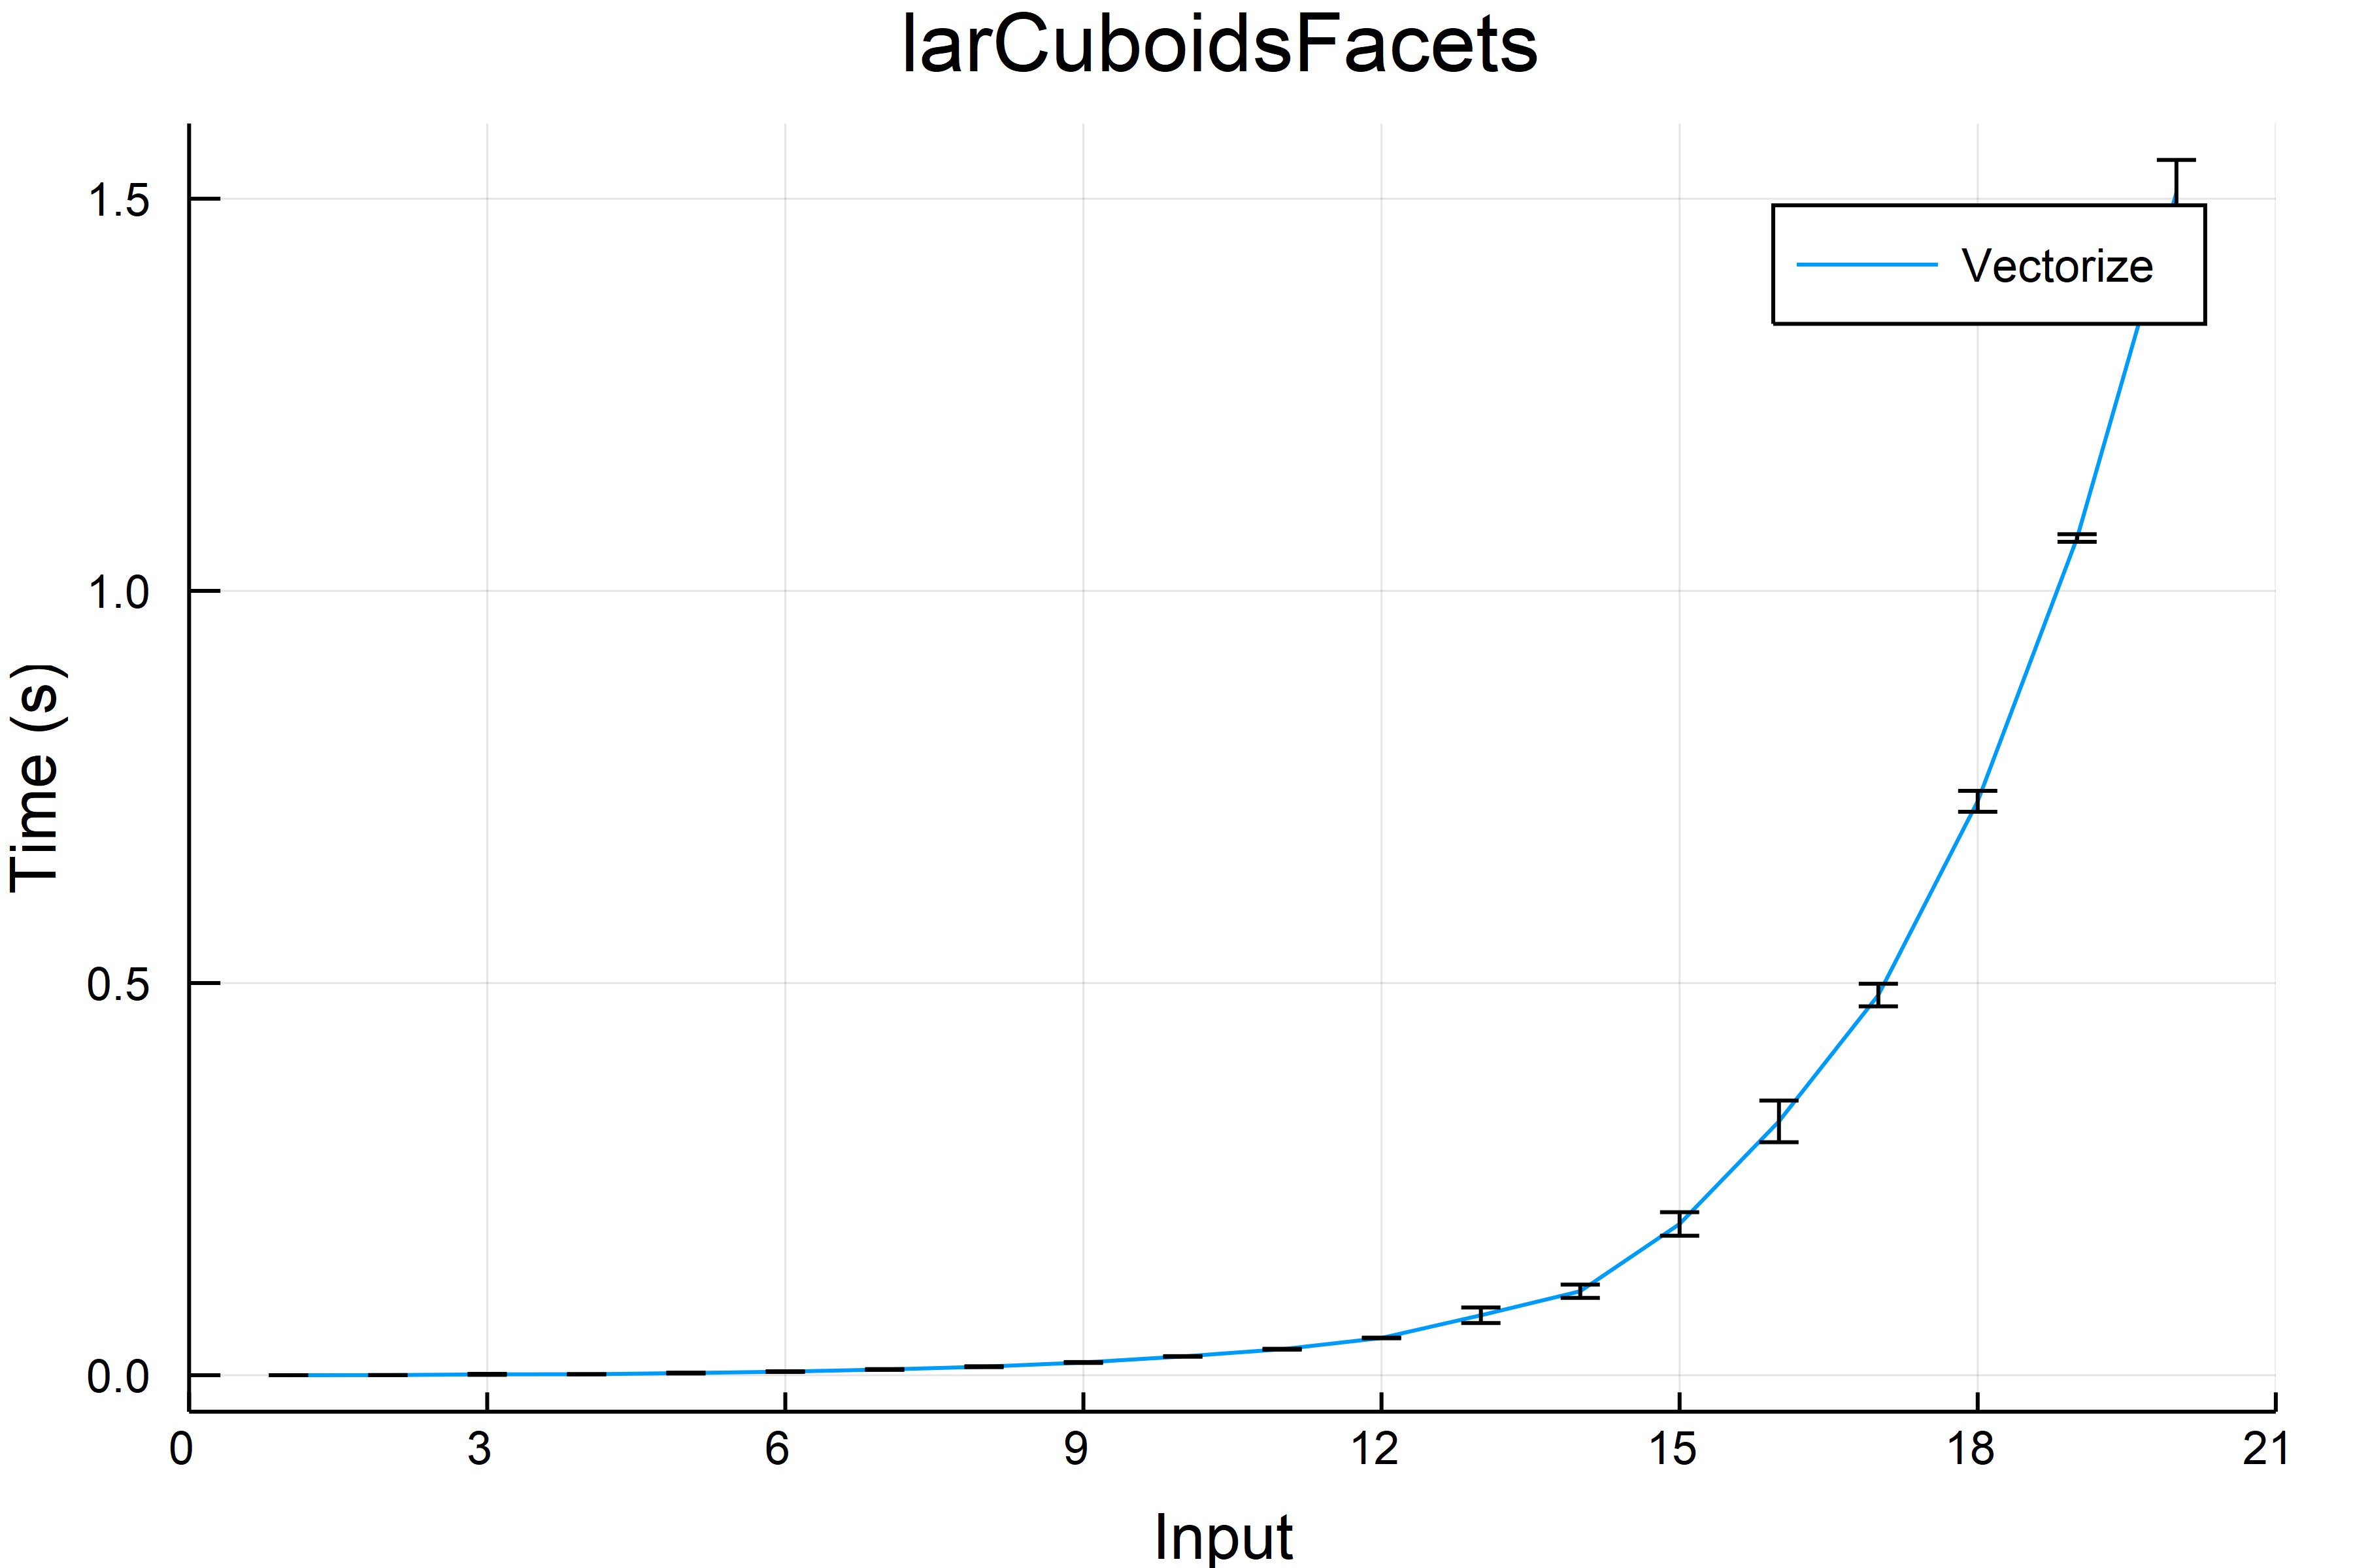
\includegraphics[scale=0.06]{larCuboidsFacetsVec.png}
\end{figure}

\paragraph{Compare}
\begin{flushleft}\small
\begin{list}{}{} \item
    \begin{Verbatim}[tabsize=4]
x=[xs,xv]
y=[ys,yv]
plot(x,y,yaxis="Time (s)",xlims = (0,length(datav)+1), xaxis="Input",
             title="larCuboidsFacets",label=["Serial" "Vectorize"],lw=1)
    \end{Verbatim}
\end{list}
\end{flushleft}  
\begin{figure}[h!]
\centering
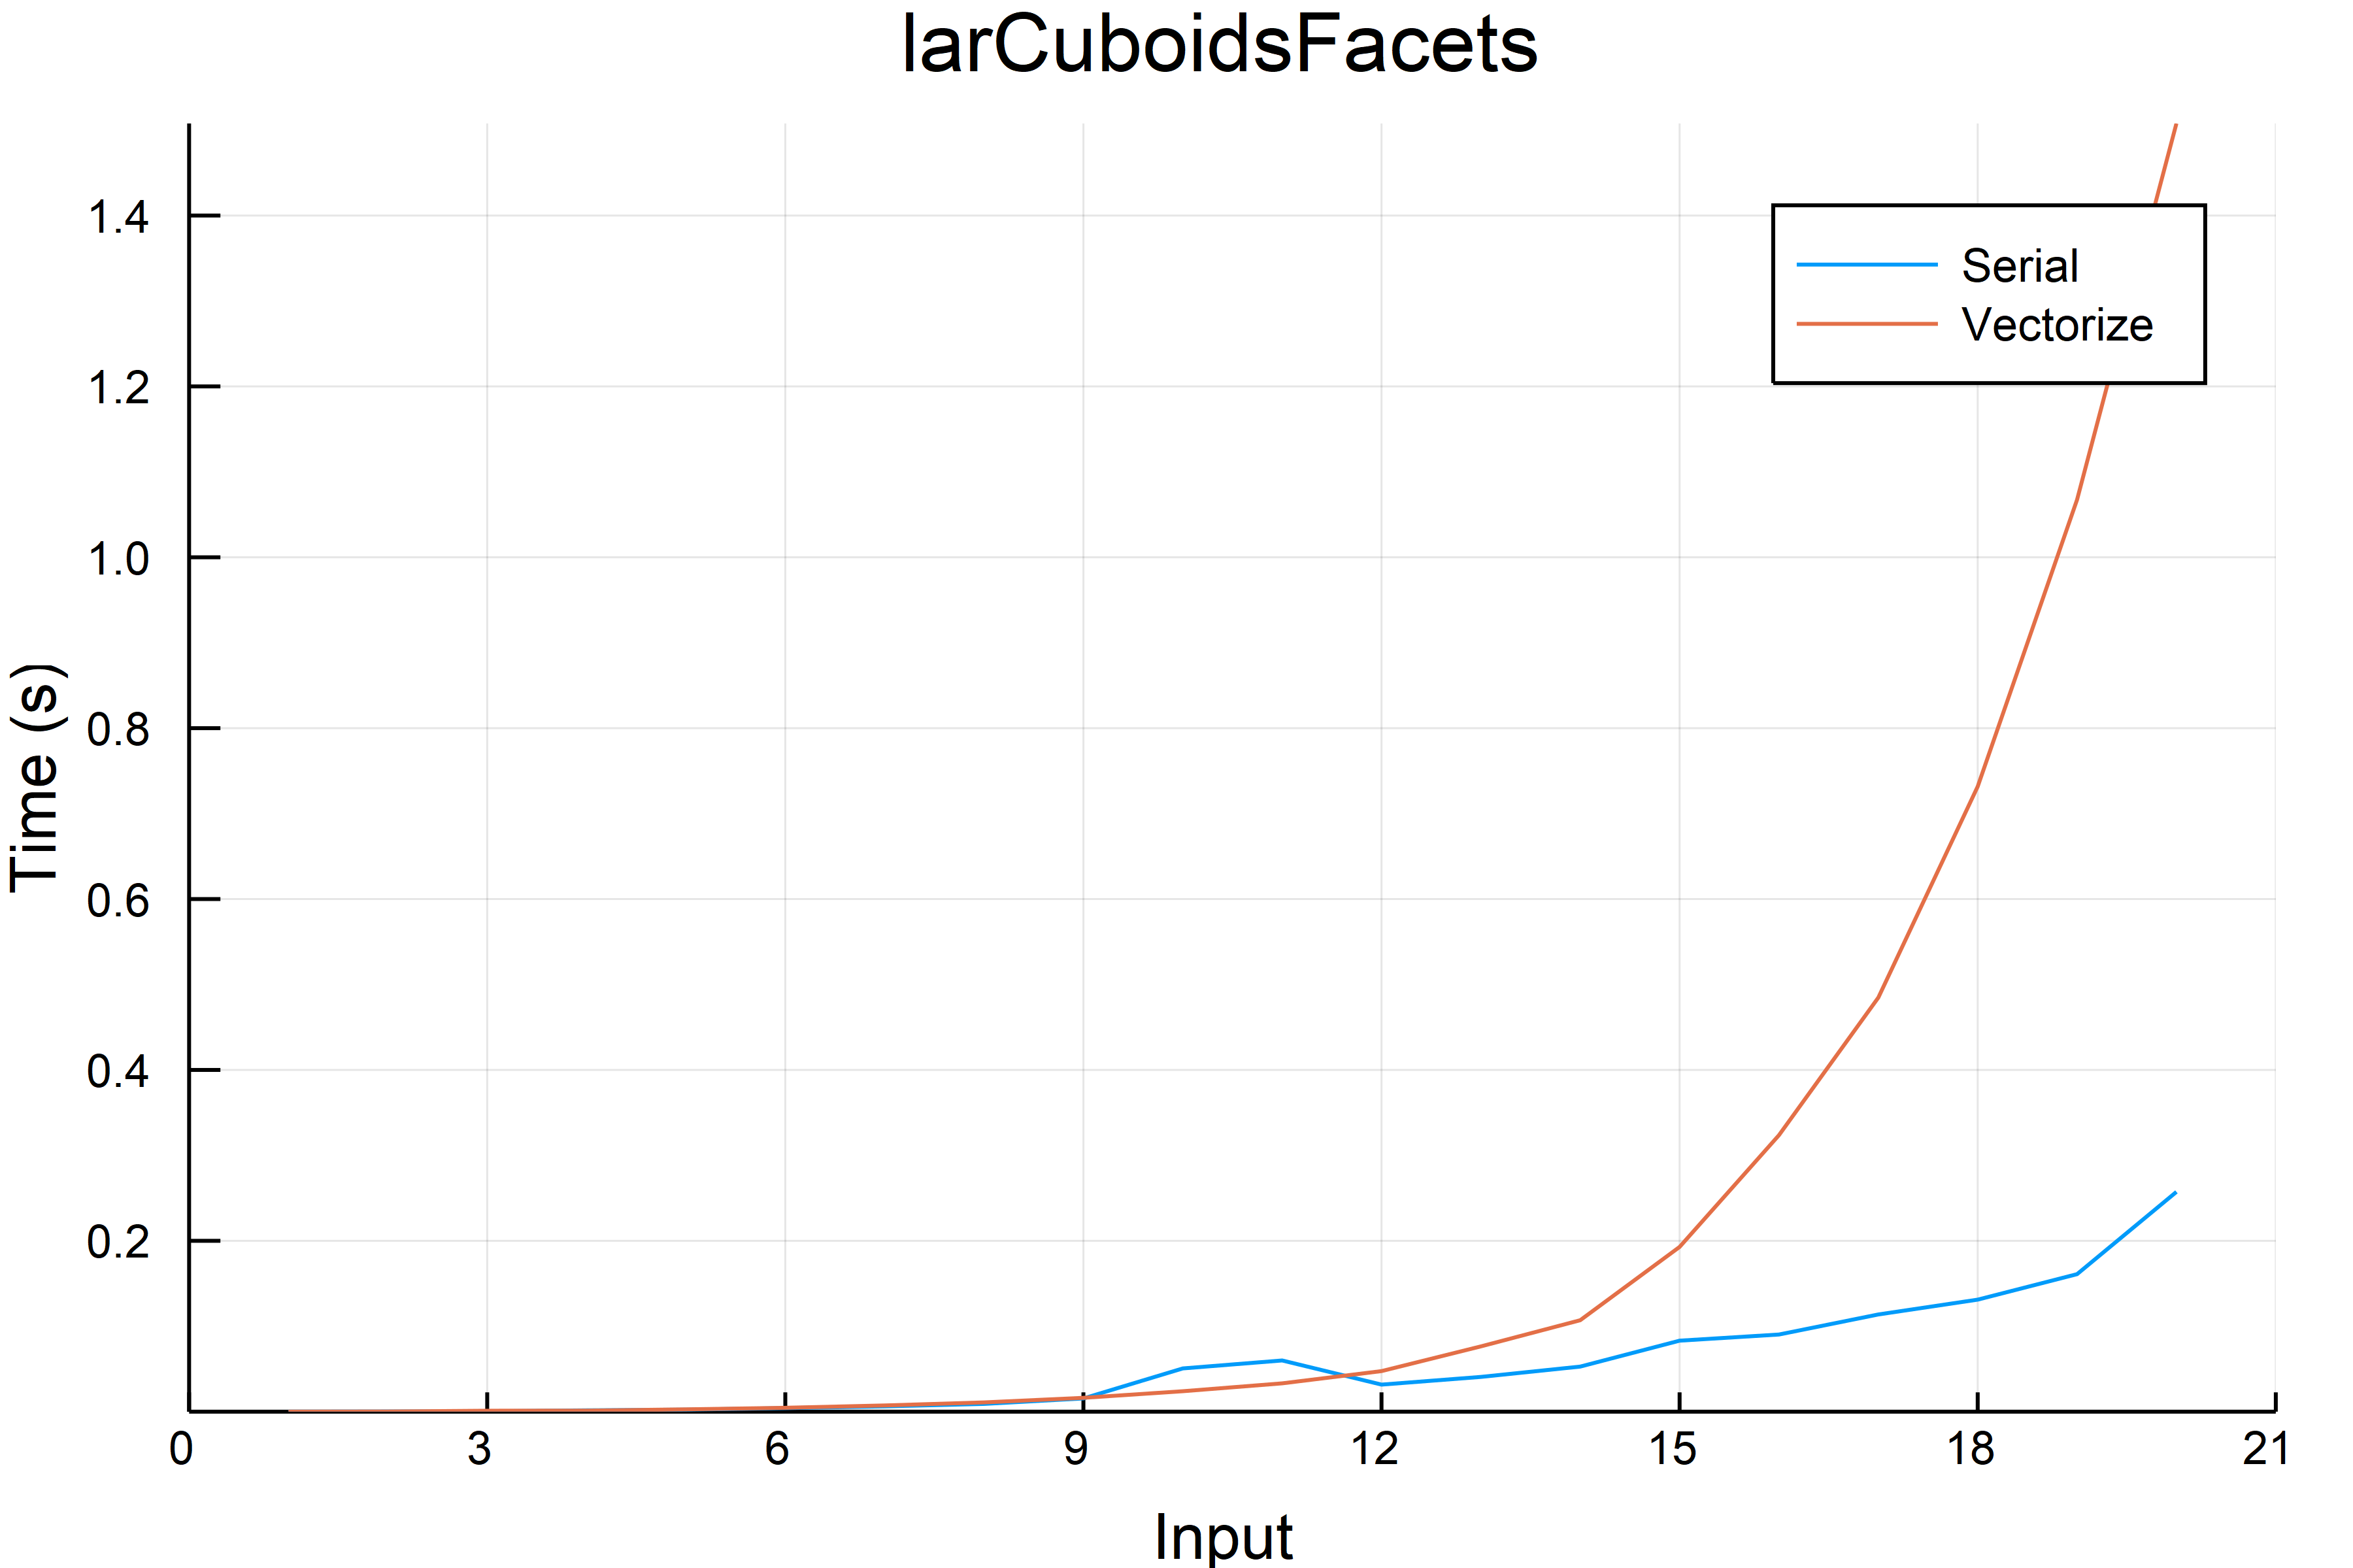
\includegraphics[scale=0.06]{larCuboidsFacetsCom1.png}
\end{figure}

The best construct to use in parallelized version seems to be the Julia standard method \texttt{pmap()}.
\paragraph{Parallel Map}
\begin{flushleft}\small
\begin{list}{}{} \item
    \begin{Verbatim}[tabsize=4]

input=[larCuboids([n,n,n]) for n in [1:6;]]

datapm=[Time(N,pmlarCuboidsFacets,j) for j in input]

xpm=[1:length(datapm);]
ypm=mean.(datapm)
yerrpm=std.(datapm)/sqrt(N)

plot(xpm,ypm,yaxis="Time (s)",xlims = (0,length(datapm)+1), yerr = yerrpm, xaxis="Input", 
                                            title="larCuboidsFacets",label=["Parallel Map"],lw=1)
    \end{Verbatim}
\end{list}
\end{flushleft} 

\paragraph{Parallel Loop}
\begin{flushleft}\small
\begin{list}{}{} \item
    \begin{Verbatim}[tabsize=4]
datap=[Time(N,plarCuboidsFacets,j) for j in input]

xp=[1:length(datap);]
yp=mean.(datap)
yerrp=std.(datap)/sqrt(N)

plot(xp,yp,yaxis="Time (s)",xlims = (0,length(datap)+1), yerr = yerrp, xaxis="Input", 
                                        title="larCuboidsFacets",label=["Parallel Loop"],lw=1)
   \end{Verbatim}
\end{list}
\end{flushleft} 
\begin{figure}[h!]
\centering
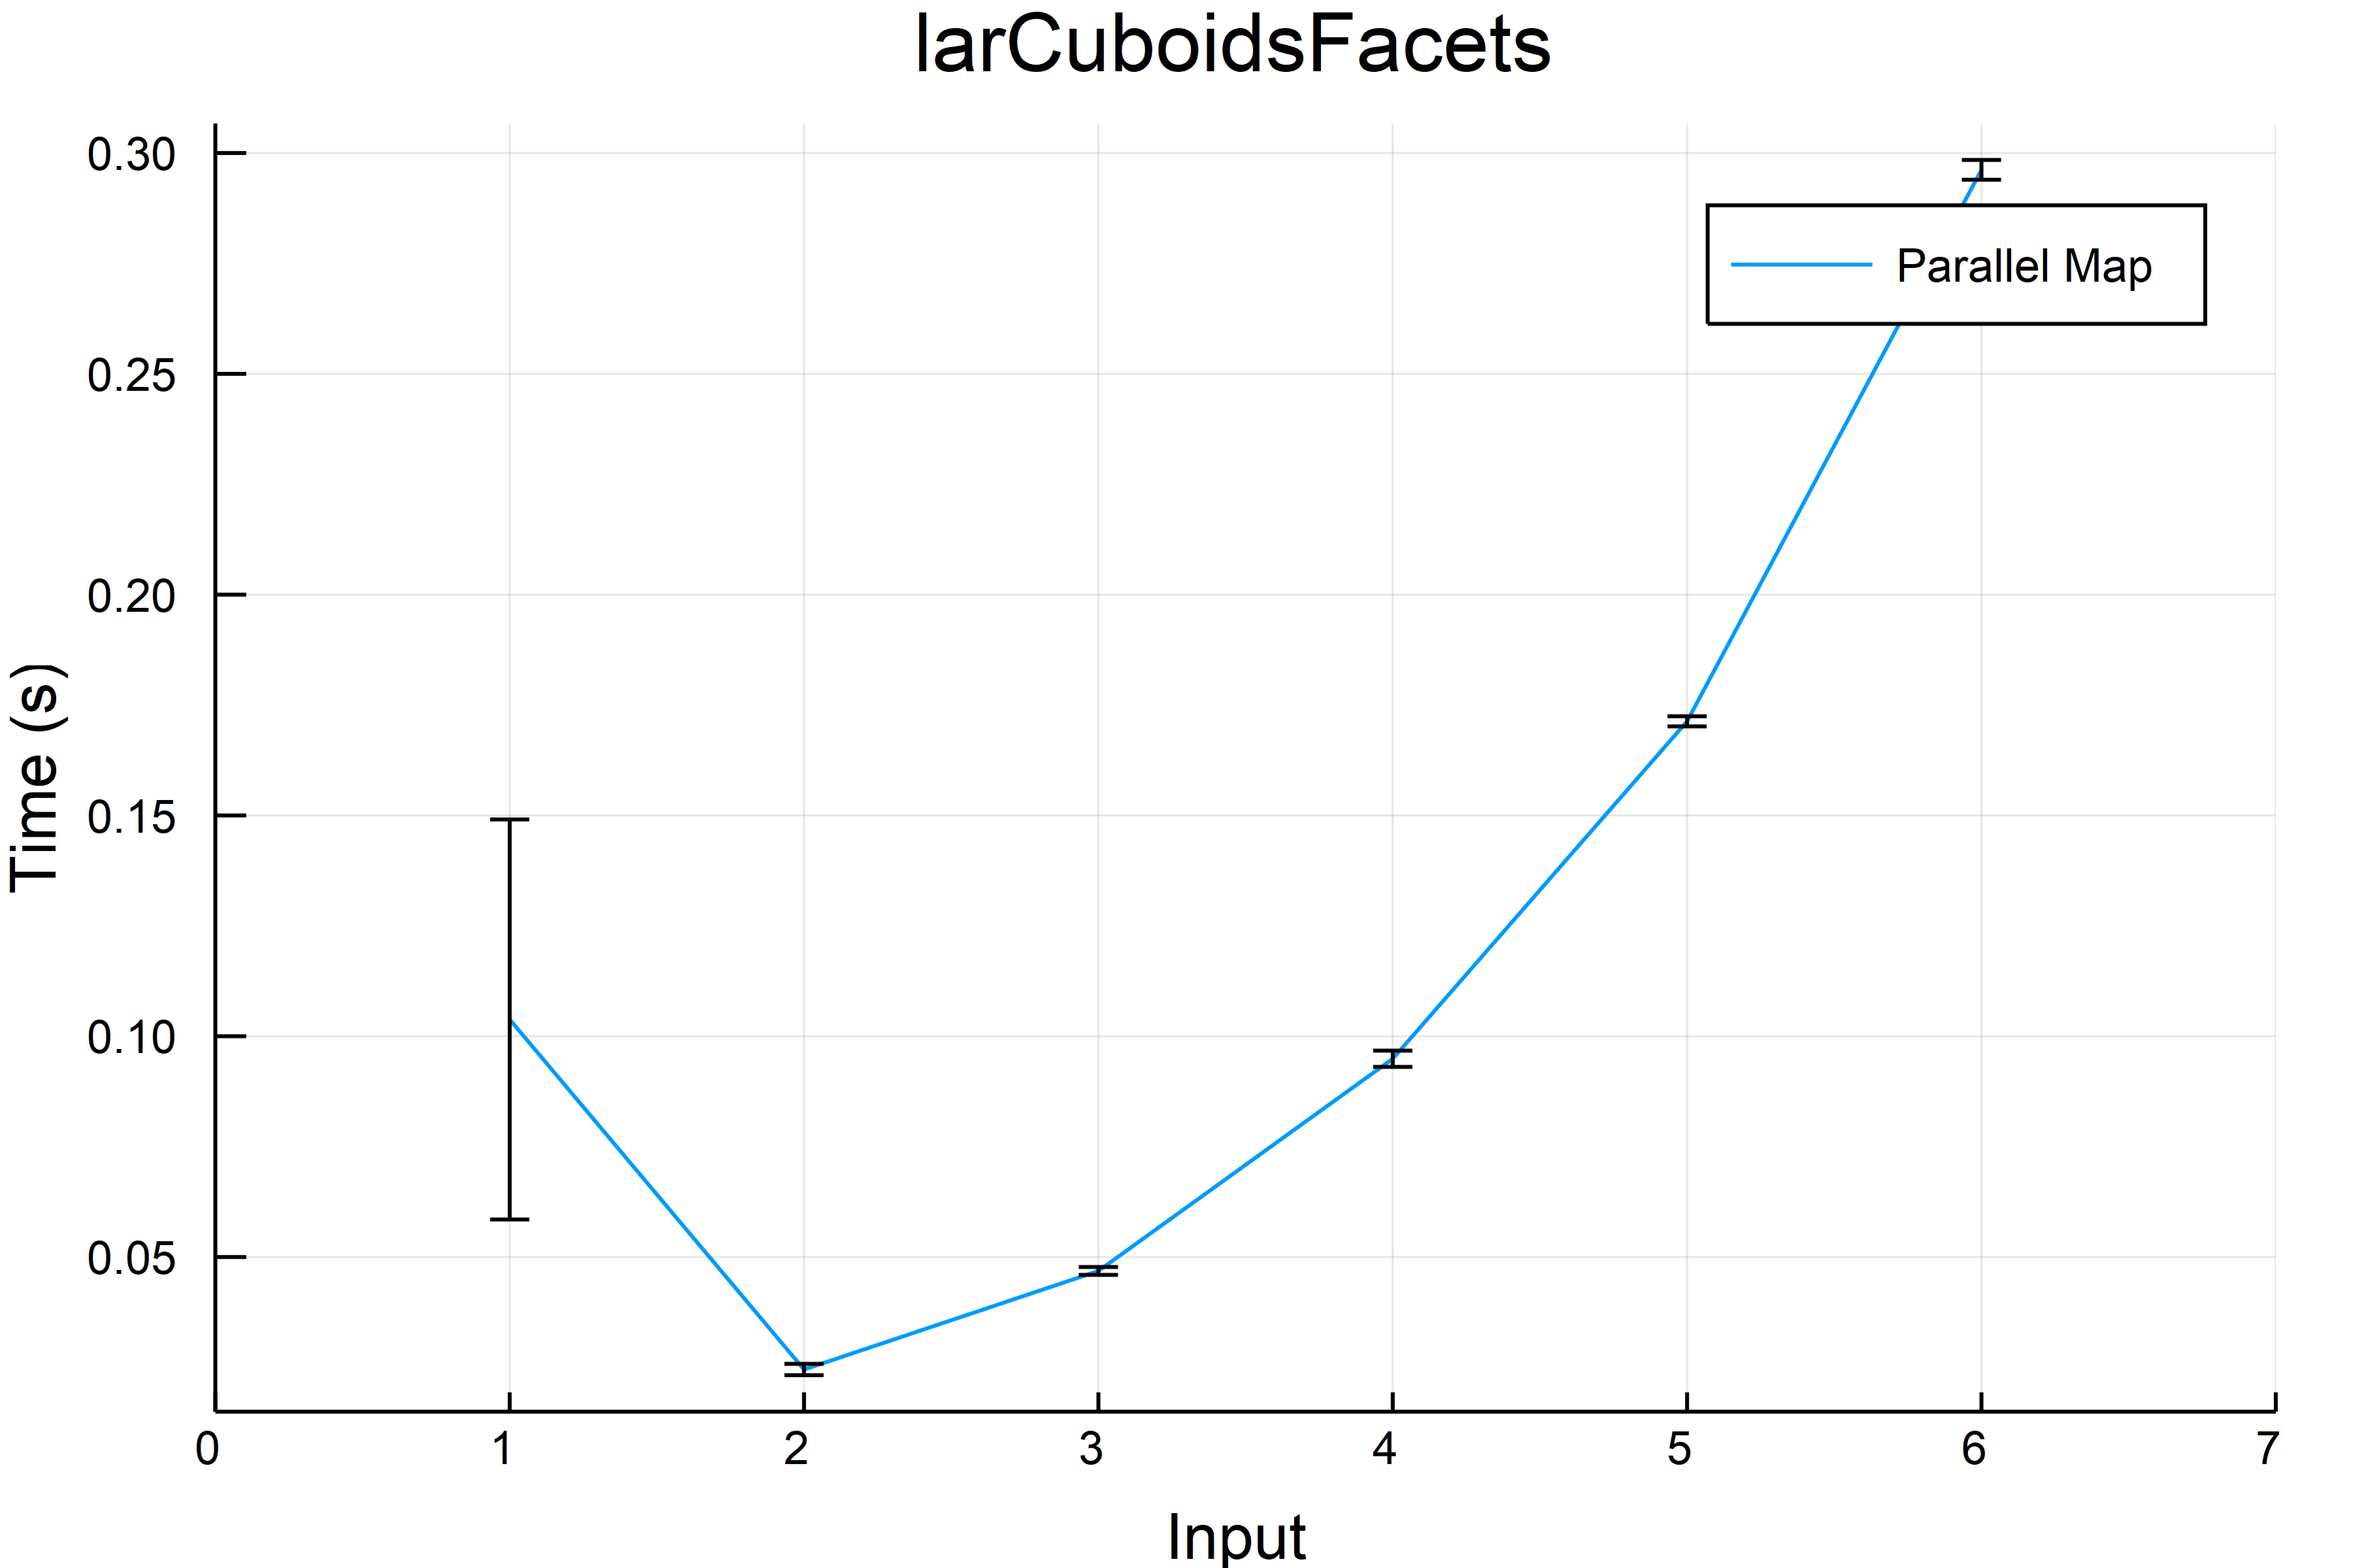
\includegraphics[scale=0.06]{larCuboidsFacetsParMap.png}
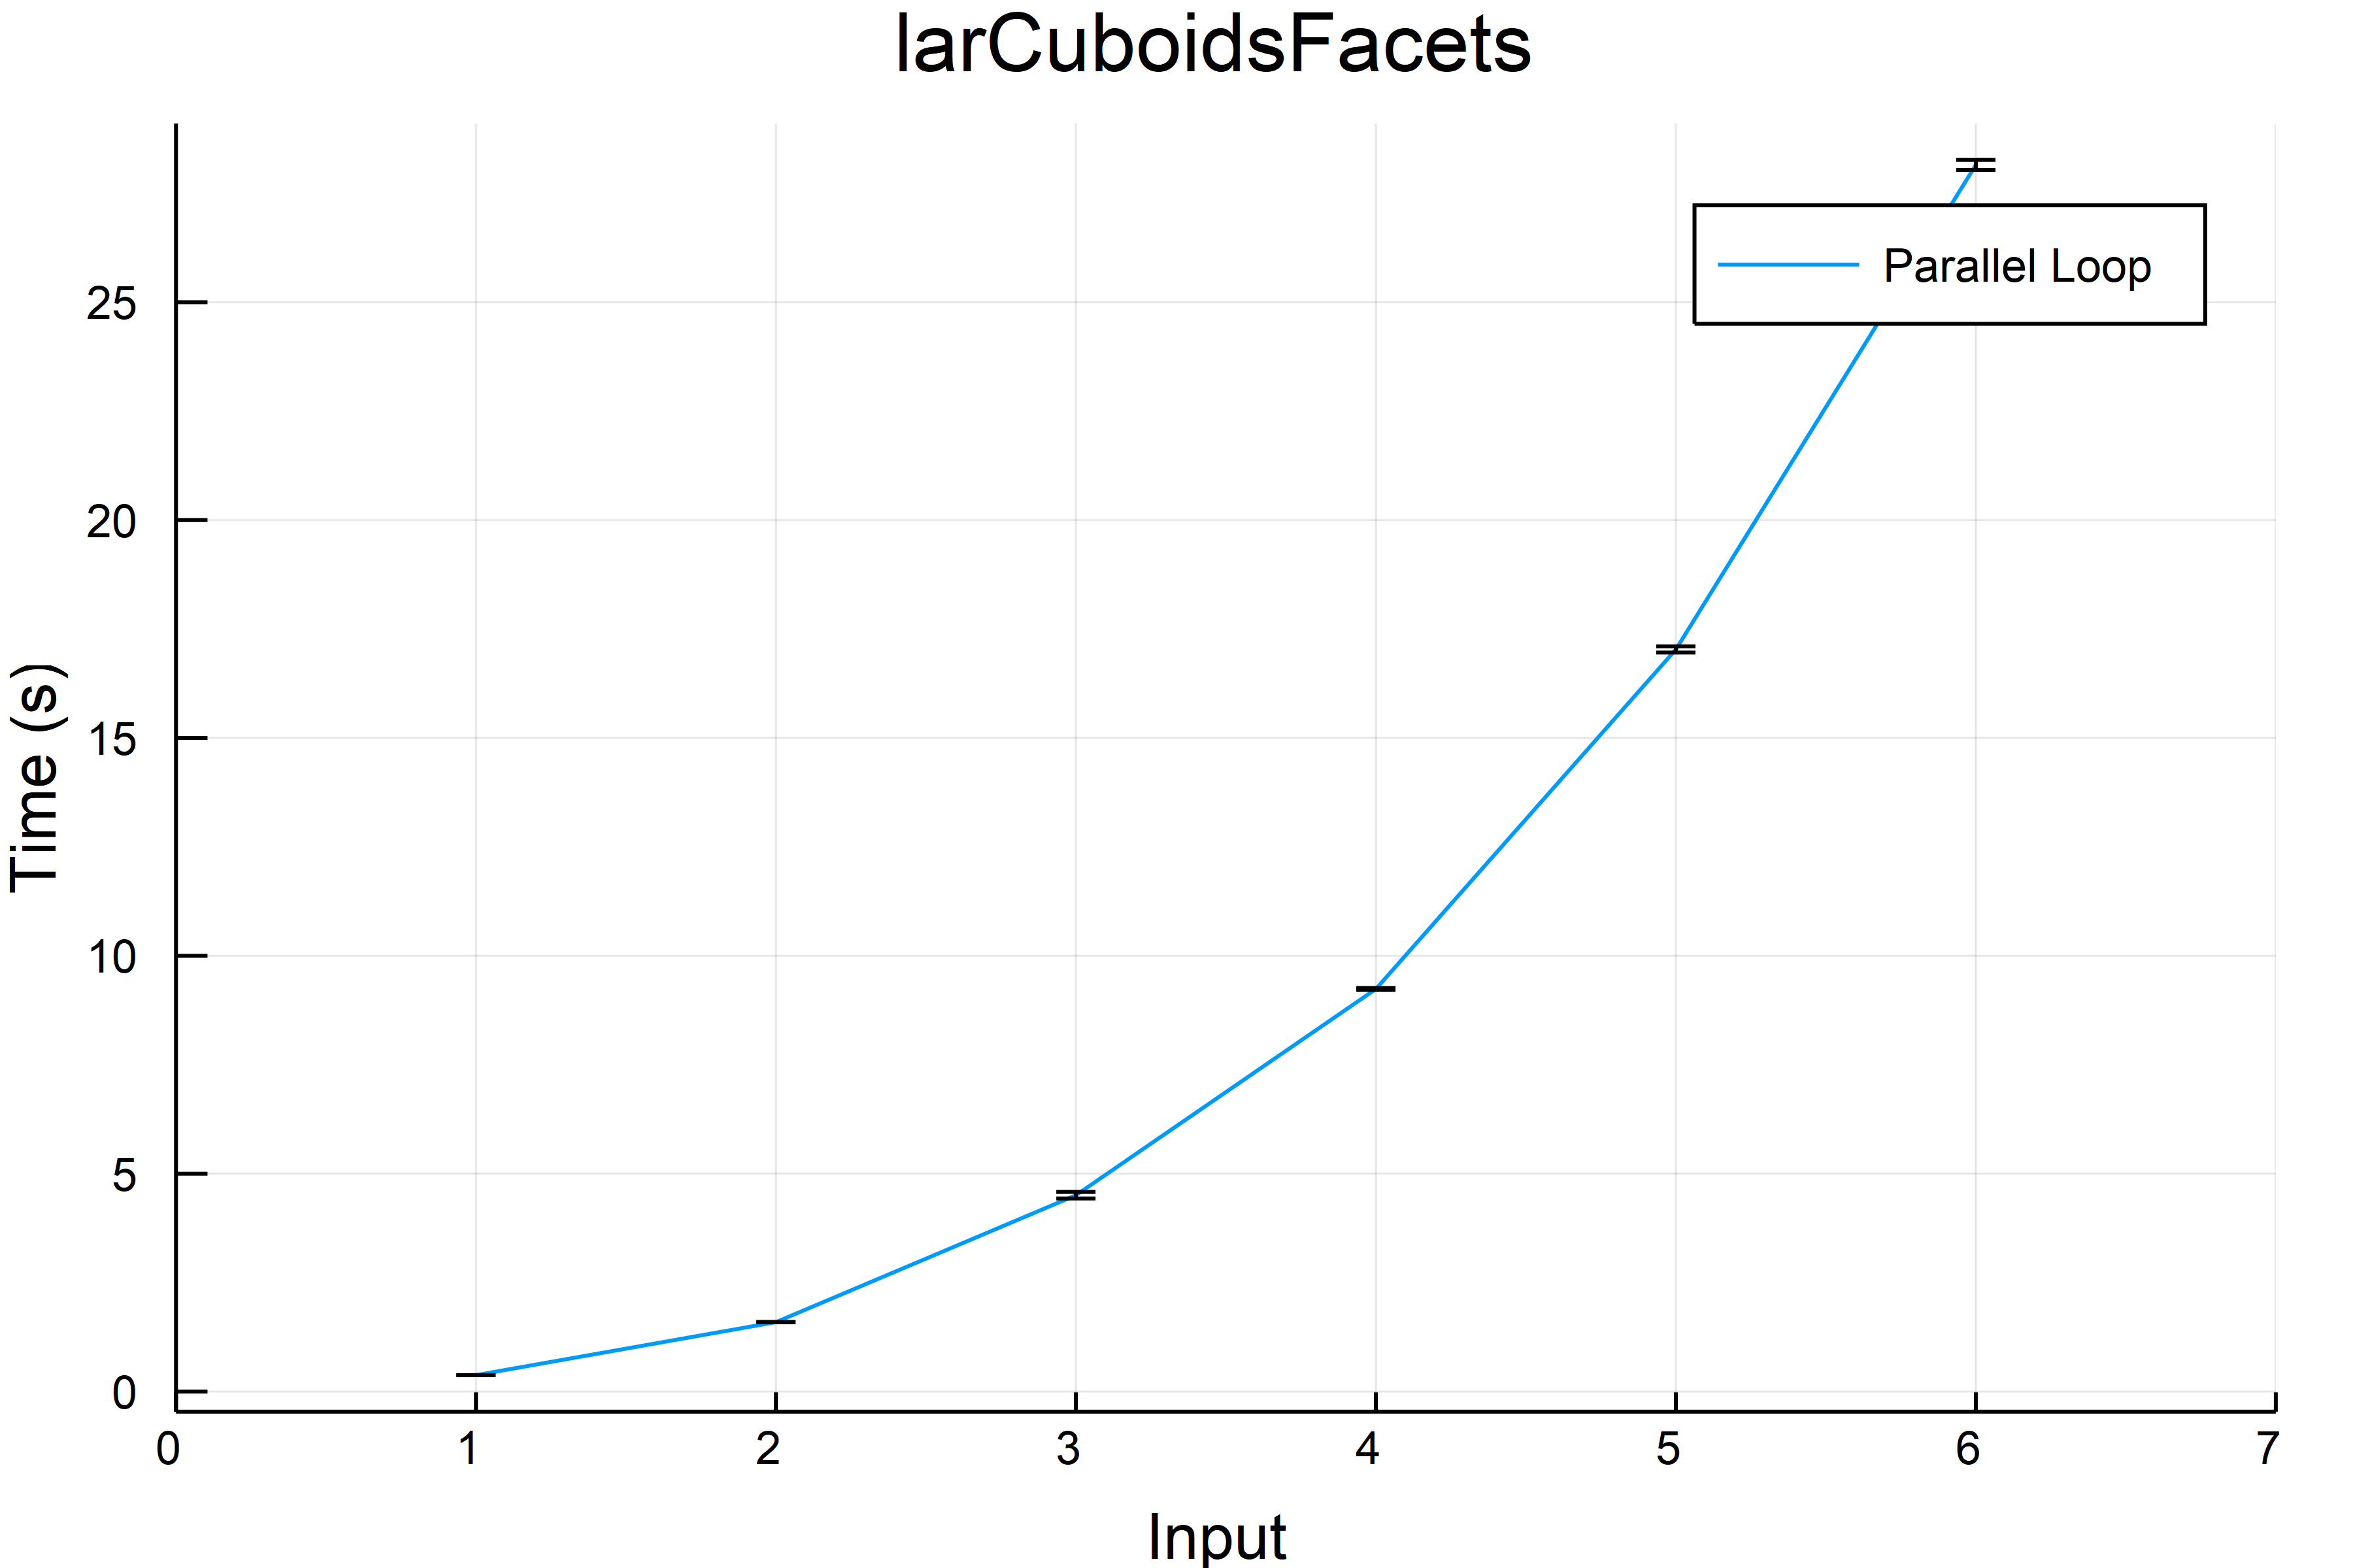
\includegraphics[scale=0.06]{larCuboidsFacetsPar.png}
\end{figure}

\paragraph{Compare}
\begin{flushleft}\small
\begin{list}{}{} \item
    \begin{Verbatim}[tabsize=4]
x=[xp, xpm]
y=[yp,ypm]

plot(x,y,yaxis="Time (s)",xlims = (0,length(datap)+1), xaxis="Input", title="larCuboidsFacets",
                                                        label=["Parallel Loop" "Parallel Map"],lw=1)
    \end{Verbatim}
\end{list}
\end{flushleft}
\begin{figure}[h!]
\centering
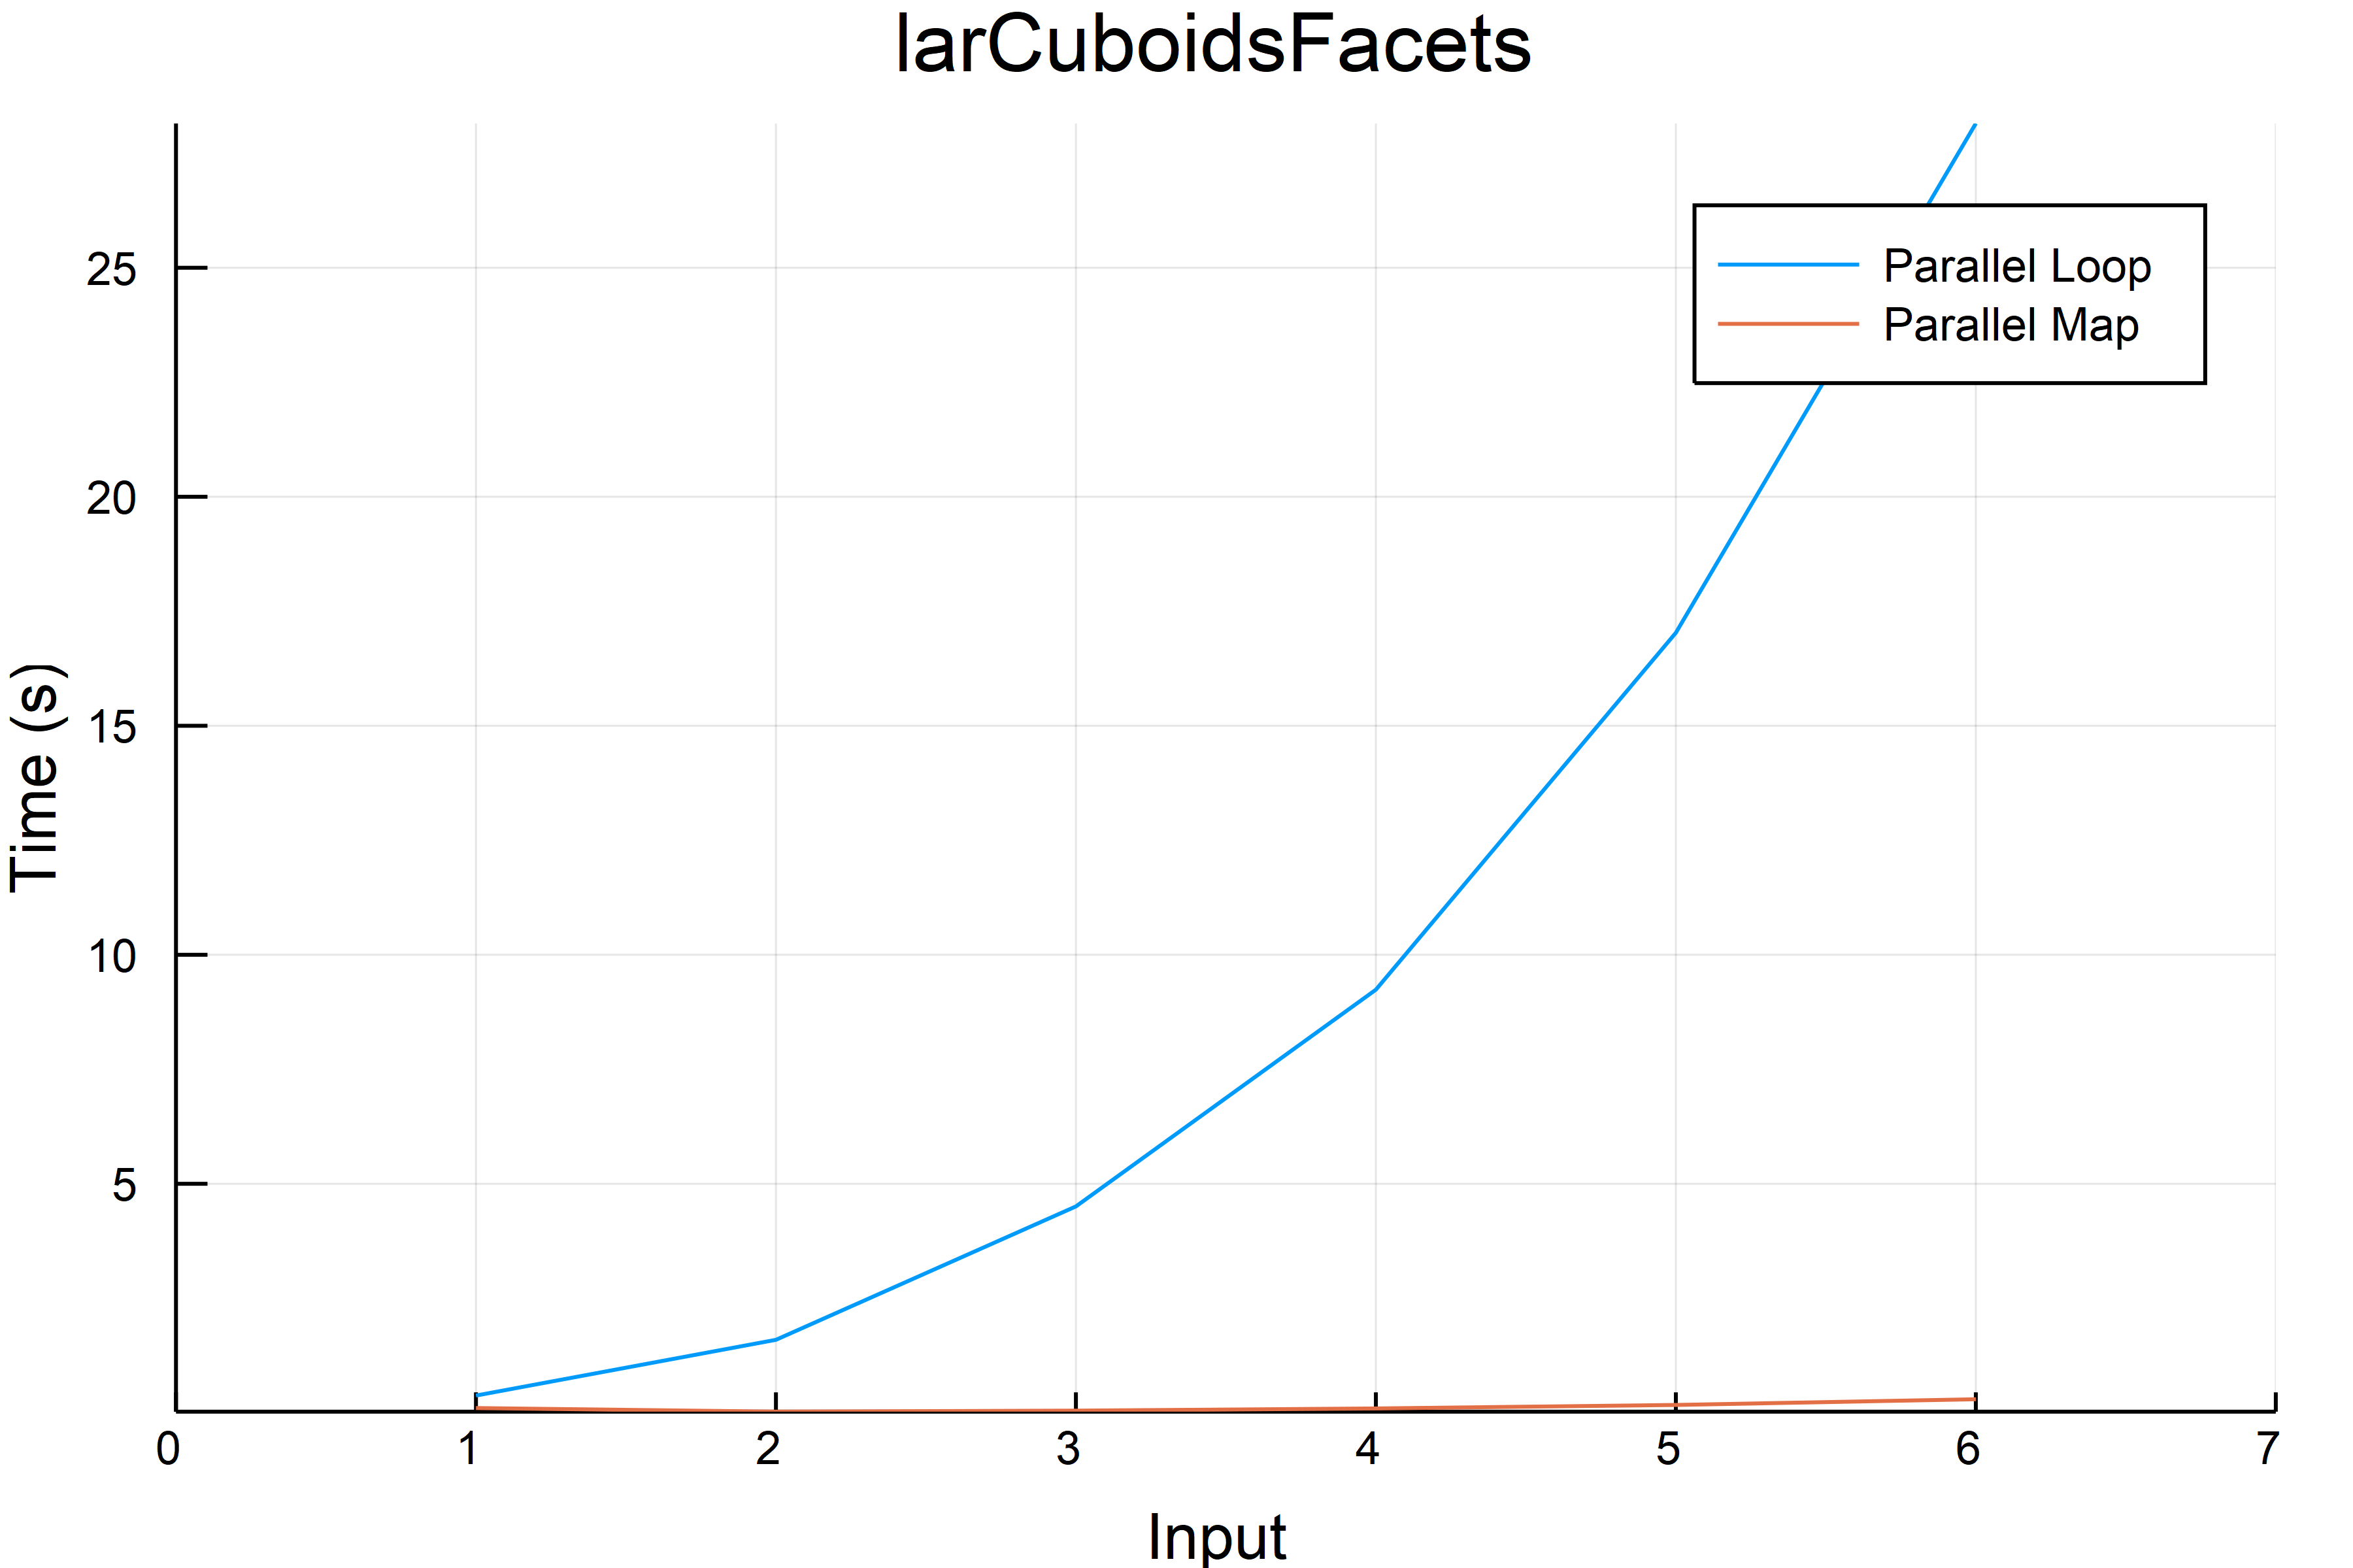
\includegraphics[scale=0.06]{larCuboidsFacetsComPar.png}
\end{figure}

\paragraph{Compare}
\begin{flushleft}\small
\begin{list}{}{} \item
    \begin{Verbatim}[tabsize=4]
x=[xs,xp]
y=[ys,yp]
plot(x,y,yaxis="Time (s)",xlims = (0,length(datas)+1), xaxis="Input", title="larCuboidsFacets",
                                                                        label=["Serial" "Parallel"],lw=1)
    \end{Verbatim}
\end{list}
\end{flushleft} 
\begin{figure}[h!]
\centering
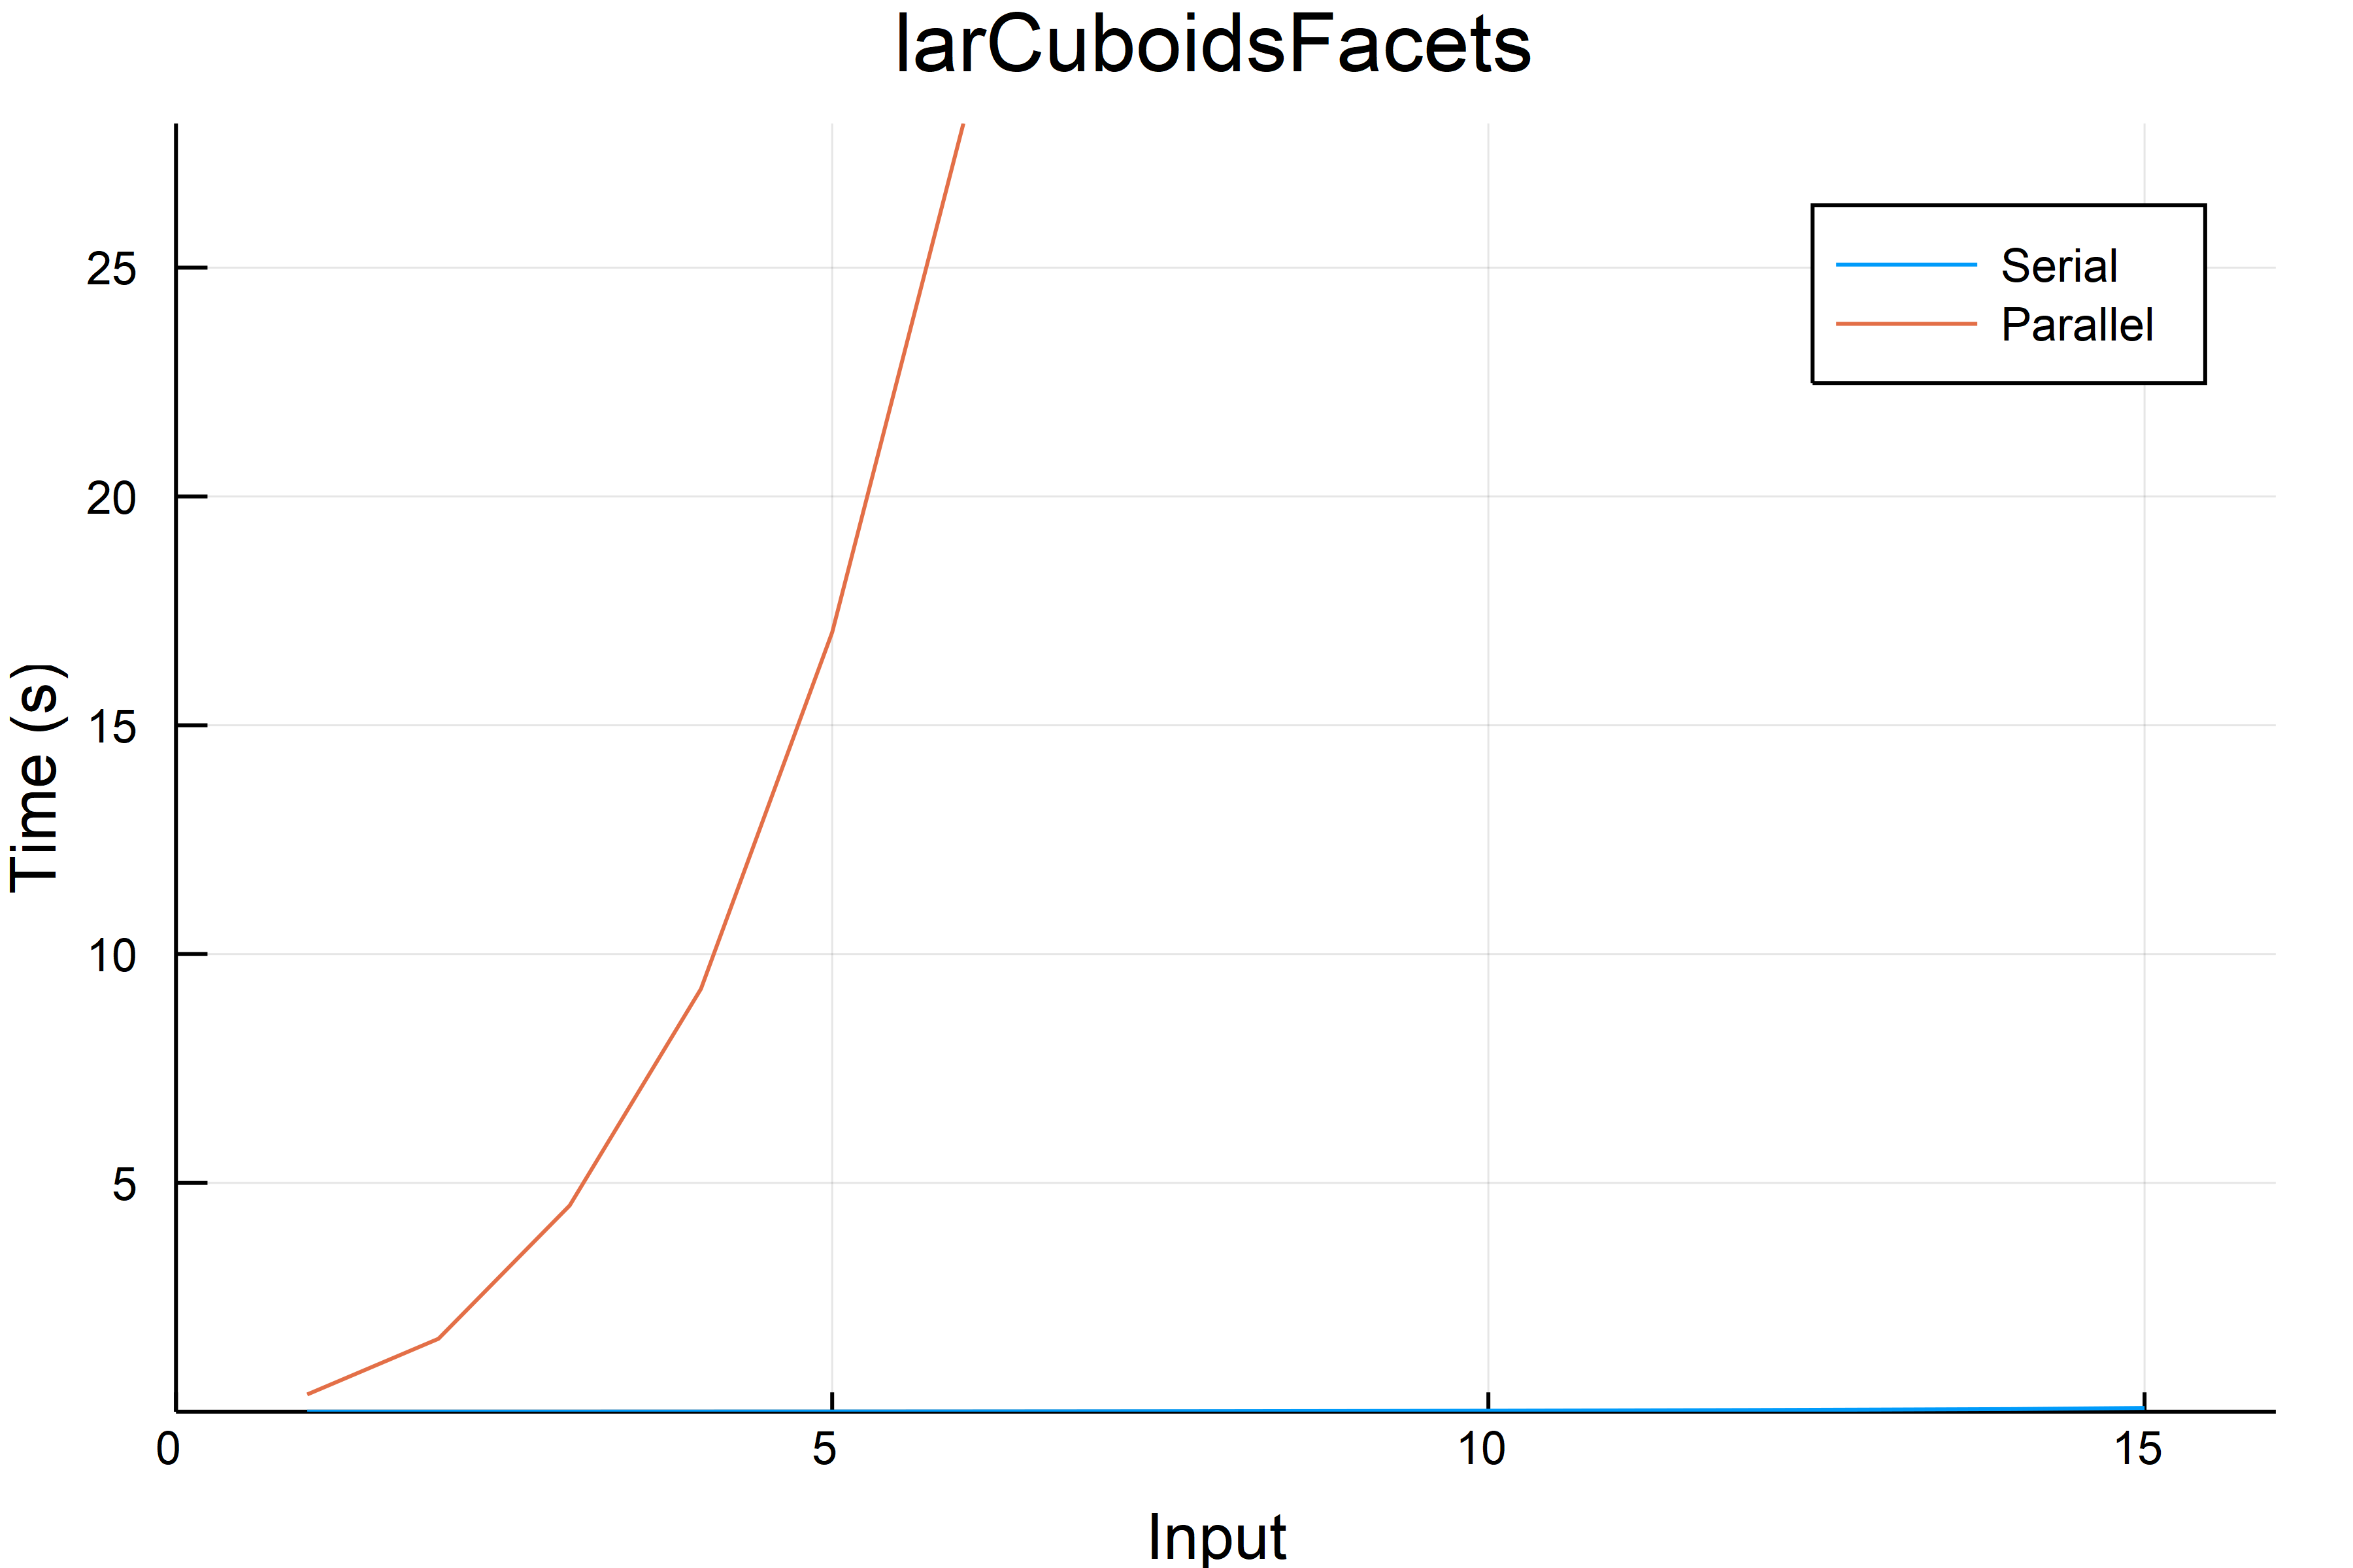
\includegraphics[scale=0.06]{larCuboidsFacetsCom.png}
\end{figure}

%-------------------------------------------------------------------------------

\subsection{larSimplicialStack:}
\vspace{1ex}
\subsubsection{Translation}
\vspace{1ex}
\begin{flushleft} \small
\begin{center}
\begin{tabular}{|p{16cm}|}
\hline
\cellcolor[gray]{.9}Python\\
\hline
\end{tabular}
\end{center}
\vspace{2ex}
\begin{list}{}{} \item
\begin{Verbatim}[tabsize=4]
def larSimplexFacets(simplices):
    out = []
    d = len(simplices[0])
    for simplex in simplices:
        out += AA(sorted)([simplex[0:k]+simplex[k+1:d] for k in range(d)])
    out = set(AA(tuple)(out))
    return  sorted(out)
    
def larSimplicialStack(simplices):
   dim = len(simplices[0])-1
   faceStack = [simplices]
   for k in range(dim):
      faces = larSimplexFacets(faceStack[-1])
      faceStack.append(faces)
   return REVERSE(faceStack)    
\end{Verbatim}
\end{list}
\vspace{2ex}
\newpage
\begin{center}
\begin{tabular}{|p{16cm}|}
\hline
\cellcolor[gray]{.9}Julia\\
\hline
\end{tabular}
\end{center}
\vspace{2ex}
\begin{list}{}{} \item
   \begin{Verbatim}[tabsize=3]
function larSimplexFacets(simplices)
	out = Array{Int64,1}[]
		d = length(simplices[1])
		for simplex in simplices
			append!(out,collect(combinations(simplex,d-1)))
		end
	return sort!(unique(out), lt=lexless)
end

function larSimplicialStack(simplices)
    dim=size(simplices[1],1)-1   
    faceStack = [simplices]
    for k in range(1,dim)
        faces = larSimplexFacets(faceStack[end])
        append!(faceStack,[faces])
    end
    return flipdim(faceStack,1)
end       
   \end{Verbatim}
\end{list}
\end{flushleft}
\vspace{2ex}
\texttt{LarSimplicialStack} function calls \texttt{larSimplexFacets} from other module. To use \texttt{combinations} you have to call the package Combinatorics by the command \texttt{using Combinatorics}. To reverse $faceStack$ is used \texttt{flipdim(A,d)} that reverse A in dimension d.
\vspace{2ex}

\subsubsection{Parallel computing}
\vspace{1ex}
\begin{flushleft} \small
\begin{center}
\begin{tabular}{|p{16cm}|}
\hline
\cellcolor[gray]{.9}Parallel\\
\hline
\end{tabular}
\end{center}
\vspace{2ex}
\begin{list}{}{} \item
   \begin{Verbatim}[tabsize=4]
@everywhere function plarSimplexFacets(simplices)
	out =  Array{Int64,1}[]
	d = length(simplices[1])
	out = @parallel (append!) for simplex in simplices
		collect(combinations(simplex,d-1))
	end
	return sort!(unique(out), lt=lexless)
end

function plarSimplicialStack(simplices)
    dim = size(simplices[1],1)-1   
    faceStack = [simplices]
    for k in range(1,dim)
        faces = plarSimplexFacets(faceStack[end])
        append!(faceStack,[faces])
    end
    return flipdim(faceStack,1)
end       
   \end{Verbatim}
\end{list}
\end{flushleft}
\vspace{2ex}
Loop inside \texttt{LarSimplicialStack} has not been further parallelized since it calls  \texttt{larSimplexFacets} on the last element added in the array, with the command \texttt{end}
\vspace{2ex}
\subsubsection{Test}
\begin{center}
\begin{tabular}{|p{16cm}|}
\hline
\cellcolor[gray]{.9}Test\\
\hline
\end{tabular}
\end{center}

\begin{flushleft}\small
\begin{list}{}{} \item
\begin{Verbatim}[tabsize=4]
@testset "larSimplicialStack Tests" begin
        @testset "euler" begin
			triang2d=[[1,2,3],[2,3,4],[3,4,5]]
            triang3d=[[1,2,3,4],[2,3,4,5],[2,4,5,6],[4,5,6,7],[3,4,5,7],[3,4,7,9],
                  [3,4,8,9],[1,3,4,8],[1,2,4,6],[1,4,6,8],[4,6,8,9],[4,6,7,9]]
            Vert2d=length(larSimplicialStack(triang2d)[1])
            Seg2d=length(larSimplicialStack(triang2d)[2])
            Fac2d=length(larSimplicialStack(triang2d)[3])
            Vert3d=length(larSimplicialStack(triang3d)[1])
            Seg3d=length(larSimplicialStack(triang3d)[2])
            Fac3d=length(larSimplicialStack(triang3d)[3])
            Cel3d=length(larSimplicialStack(triang3d)[4])
                @test Vert2d-Seg2d+Fac2d == 1
                @test Vert3d-Seg3d+Fac3d-Cel3d == 1
		end
		
		@testset "proof" begin
			@testset "$shape" for shape in [[1,2,3,4],[2,3,4,5,6]]
				@test length(larSimplicialStack([shape])) == length(shape)
				@test typeof(larSimplicialStack([shape])) == Array{Array{Array{Int64,1},1},1}
			end
		end
end	
	
@testset "plarSimplicialStack Tests" begin
            @testset "euler" begin
    			triang2d=[[1,2,3],[2,3,4],[3,4,5]]
                triang3d=[[1,2,3,4],[2,3,4,5],[2,4,5,6],[4,5,6,7],[3,4,5,7],[3,4,7,9],
                      [3,4,8,9],[1,3,4,8],[1,2,4,6],[1,4,6,8],[4,6,8,9],[4,6,7,9]]
                Vert2d=length(plarSimplicialStack(triang2d)[1])
                Seg2d=length(plarSimplicialStack(triang2d)[2])
                Fac2d=length(plarSimplicialStack(triang2d)[3])
                Vert3d=length(plarSimplicialStack(triang3d)[1])
                Seg3d=length(plarSimplicialStack(triang3d)[2])
                Fac3d=length(plarSimplicialStack(triang3d)[3])
                Cel3d=length(plarSimplicialStack(triang3d)[4])
                    @test Vert2d-Seg2d+Fac2d == 1
                    @test Vert3d-Seg3d+Fac3d-Cel3d == 1
    		end
		
	    	@testset "proof" begin
		    	@testset "$shape" for shape in [[1,2,3,4],[2,3,4,5,6]]
			    	@test length(plarSimplicialStack([shape])) == length(shape)
				    @test typeof(plarSimplicialStack([shape])) ==  Array{Array{Array{Int64,1},1},1}
			    end
		    end
end	

\end{Verbatim}
\end{list}
\end{flushleft}

\subsubsection{Execution time}
\begin{center}
\begin{tabular}{|p{16cm}|}
\hline
\cellcolor[gray]{.9}Execution time\\
\hline
\end{tabular}
\end{center}



\paragraph{Serial}
\begin{flushleft}\small
\begin{list}{}{} \item
    \begin{Verbatim}[tabsize=4]
datas=[Time(N,larSimplicialStack,[[1:j;]]) for j in range(4,15)]
xs=[1:length(datas);]
ys=mean.(datas)
yerrs=std.(datas)/sqrt(N)
plot(xs,ys,yaxis="Time (s)",xlims = (0,length(datas)+1), yerr = yerrs, xaxis="Input",
                                            title="larSimplicialStack",label=["Serial"],lw=1)
    \end{Verbatim}
\end{list}
\end{flushleft} 

\paragraph{Parallel}
\begin{flushleft}\small
\begin{list}{}{} \item
    \begin{Verbatim}[tabsize=4]
datap=[Time(N,plarSimplicialStack,[[1:j;]]) for j in range(4,15)]
xp=[1:length(datap);]
yp=mean.(datap)
yerrp=std.(datap)/sqrt(N)
plot(xp,yp,yaxis="Time (s)",xlims = (0,length(datap)+1), yerr = yerrp, xaxis="Input",
                                        title="larSimplicialStack",label=["Parallel"],lw=1)
    \end{Verbatim}
\end{list}
\end{flushleft}
\begin{figure}[h!]
\centering
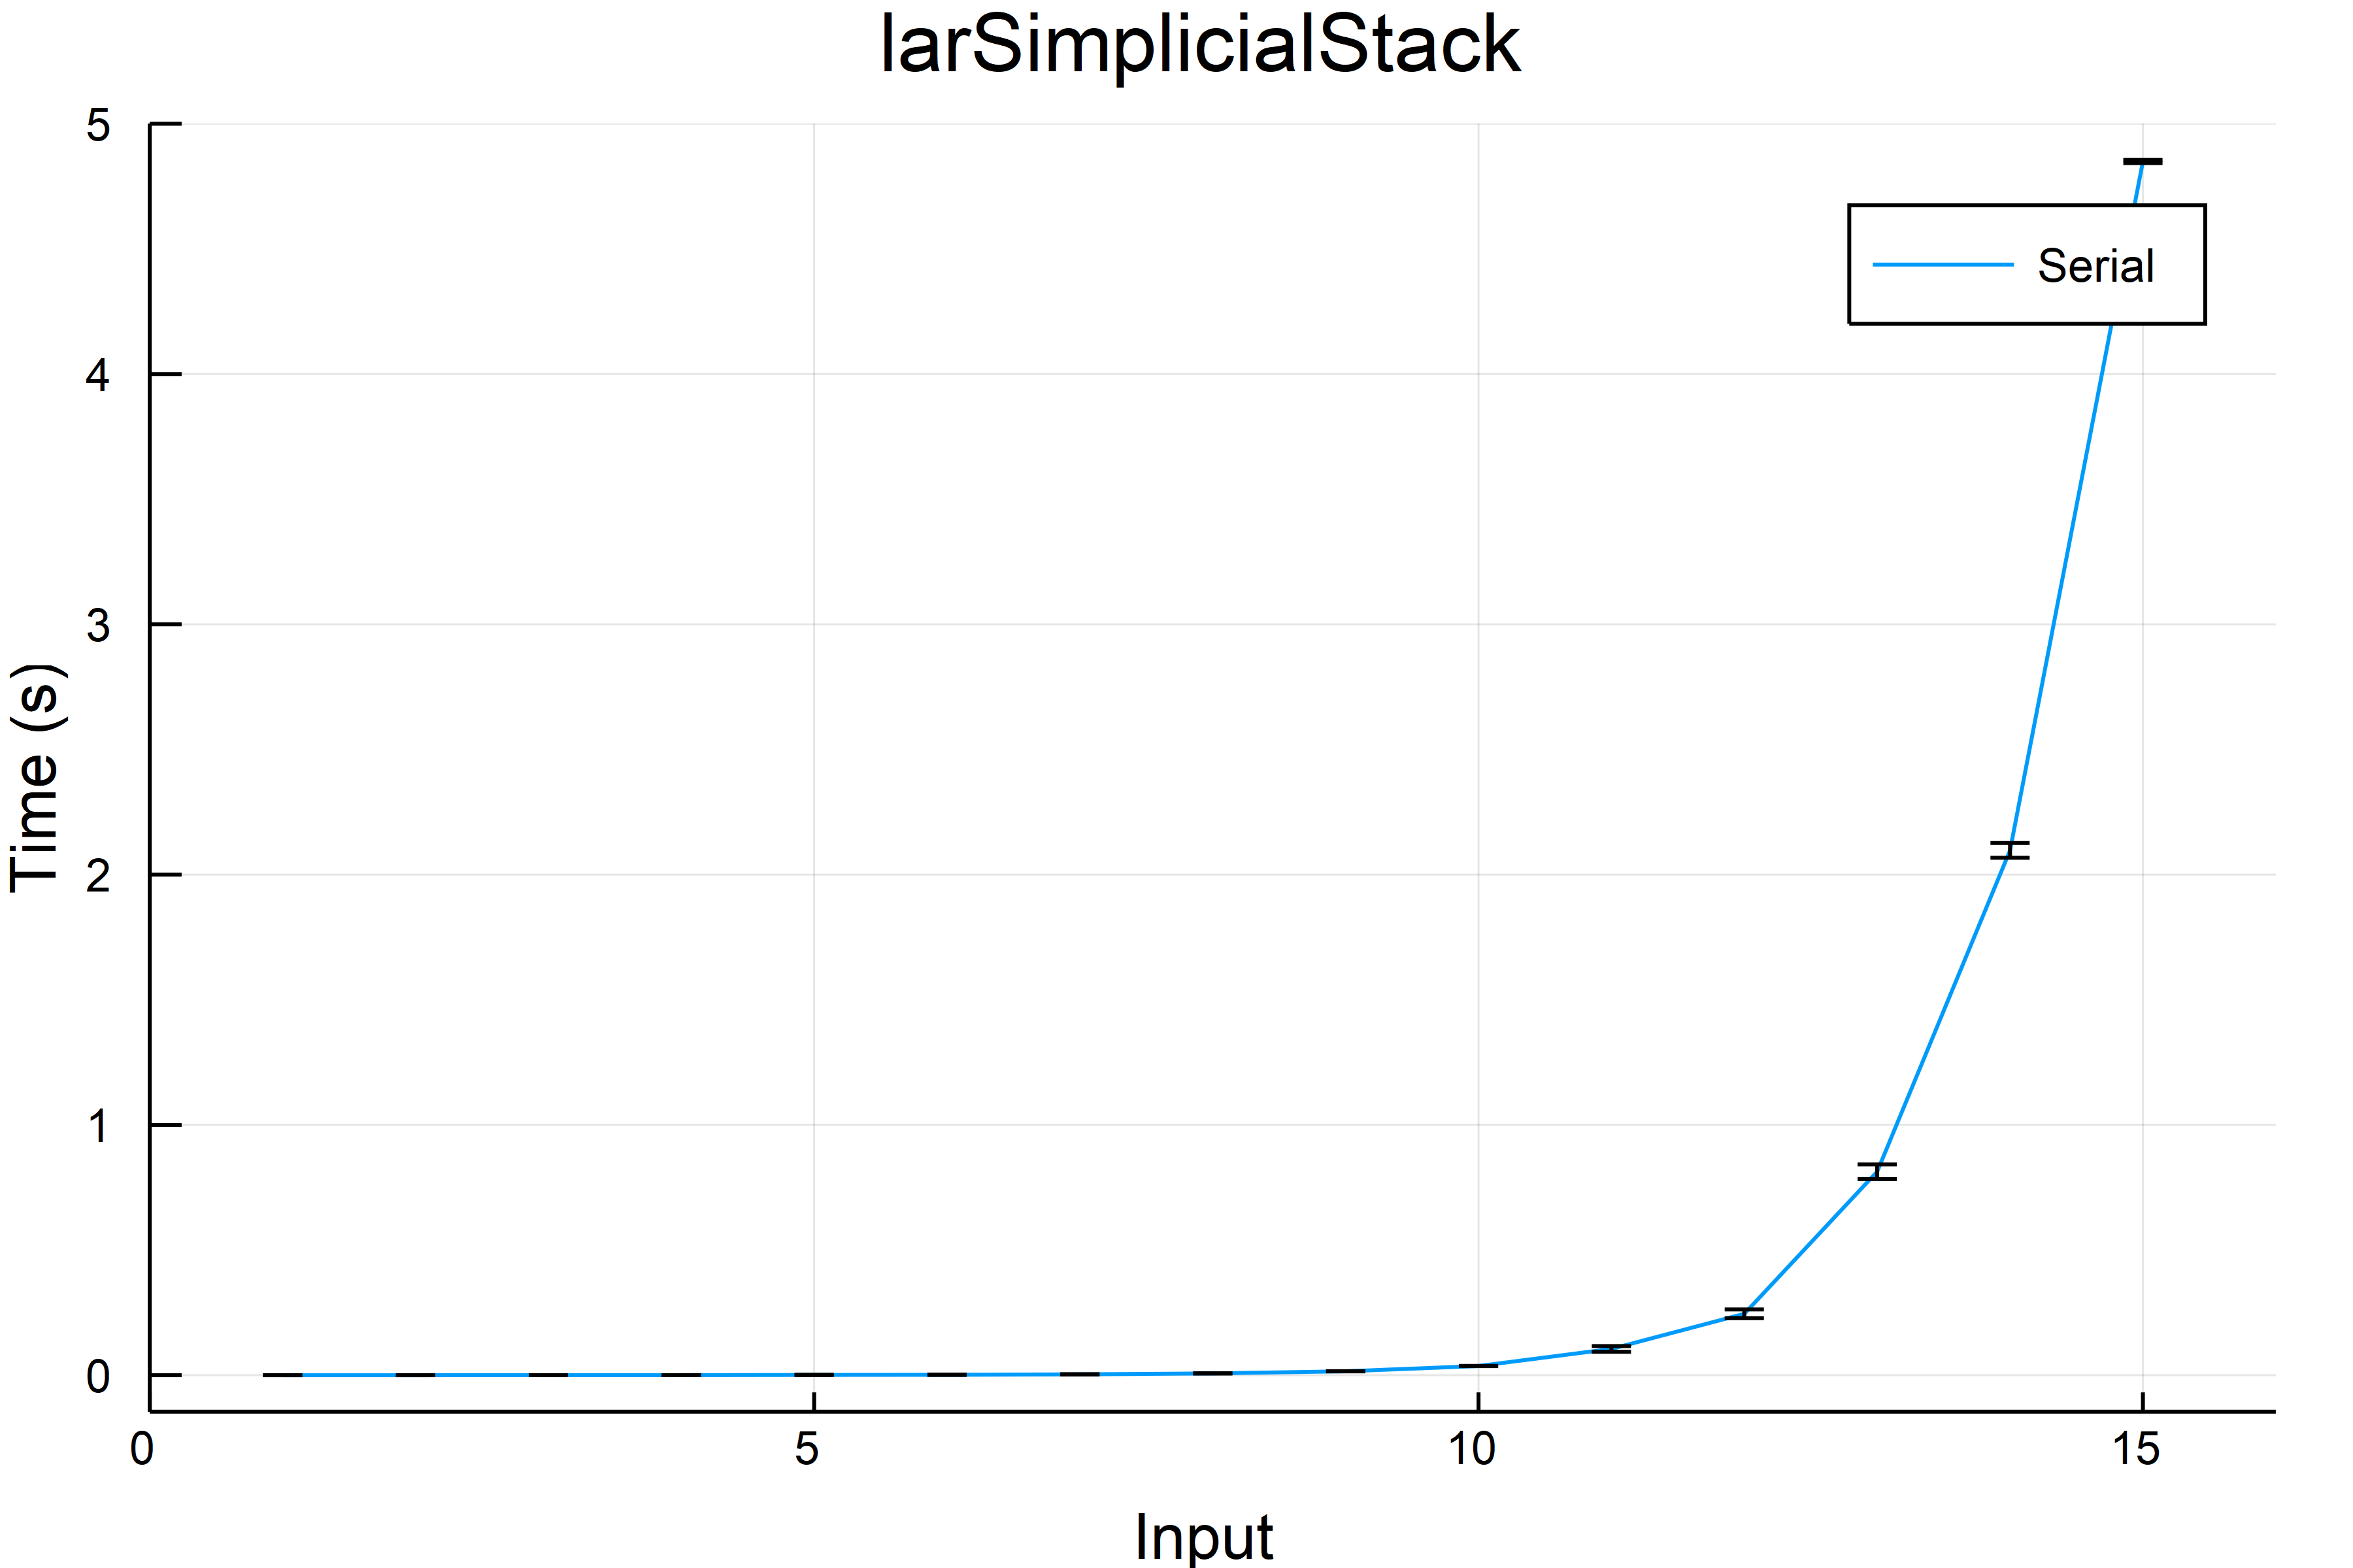
\includegraphics[scale=0.06]{larSimplicialStackSer.png}
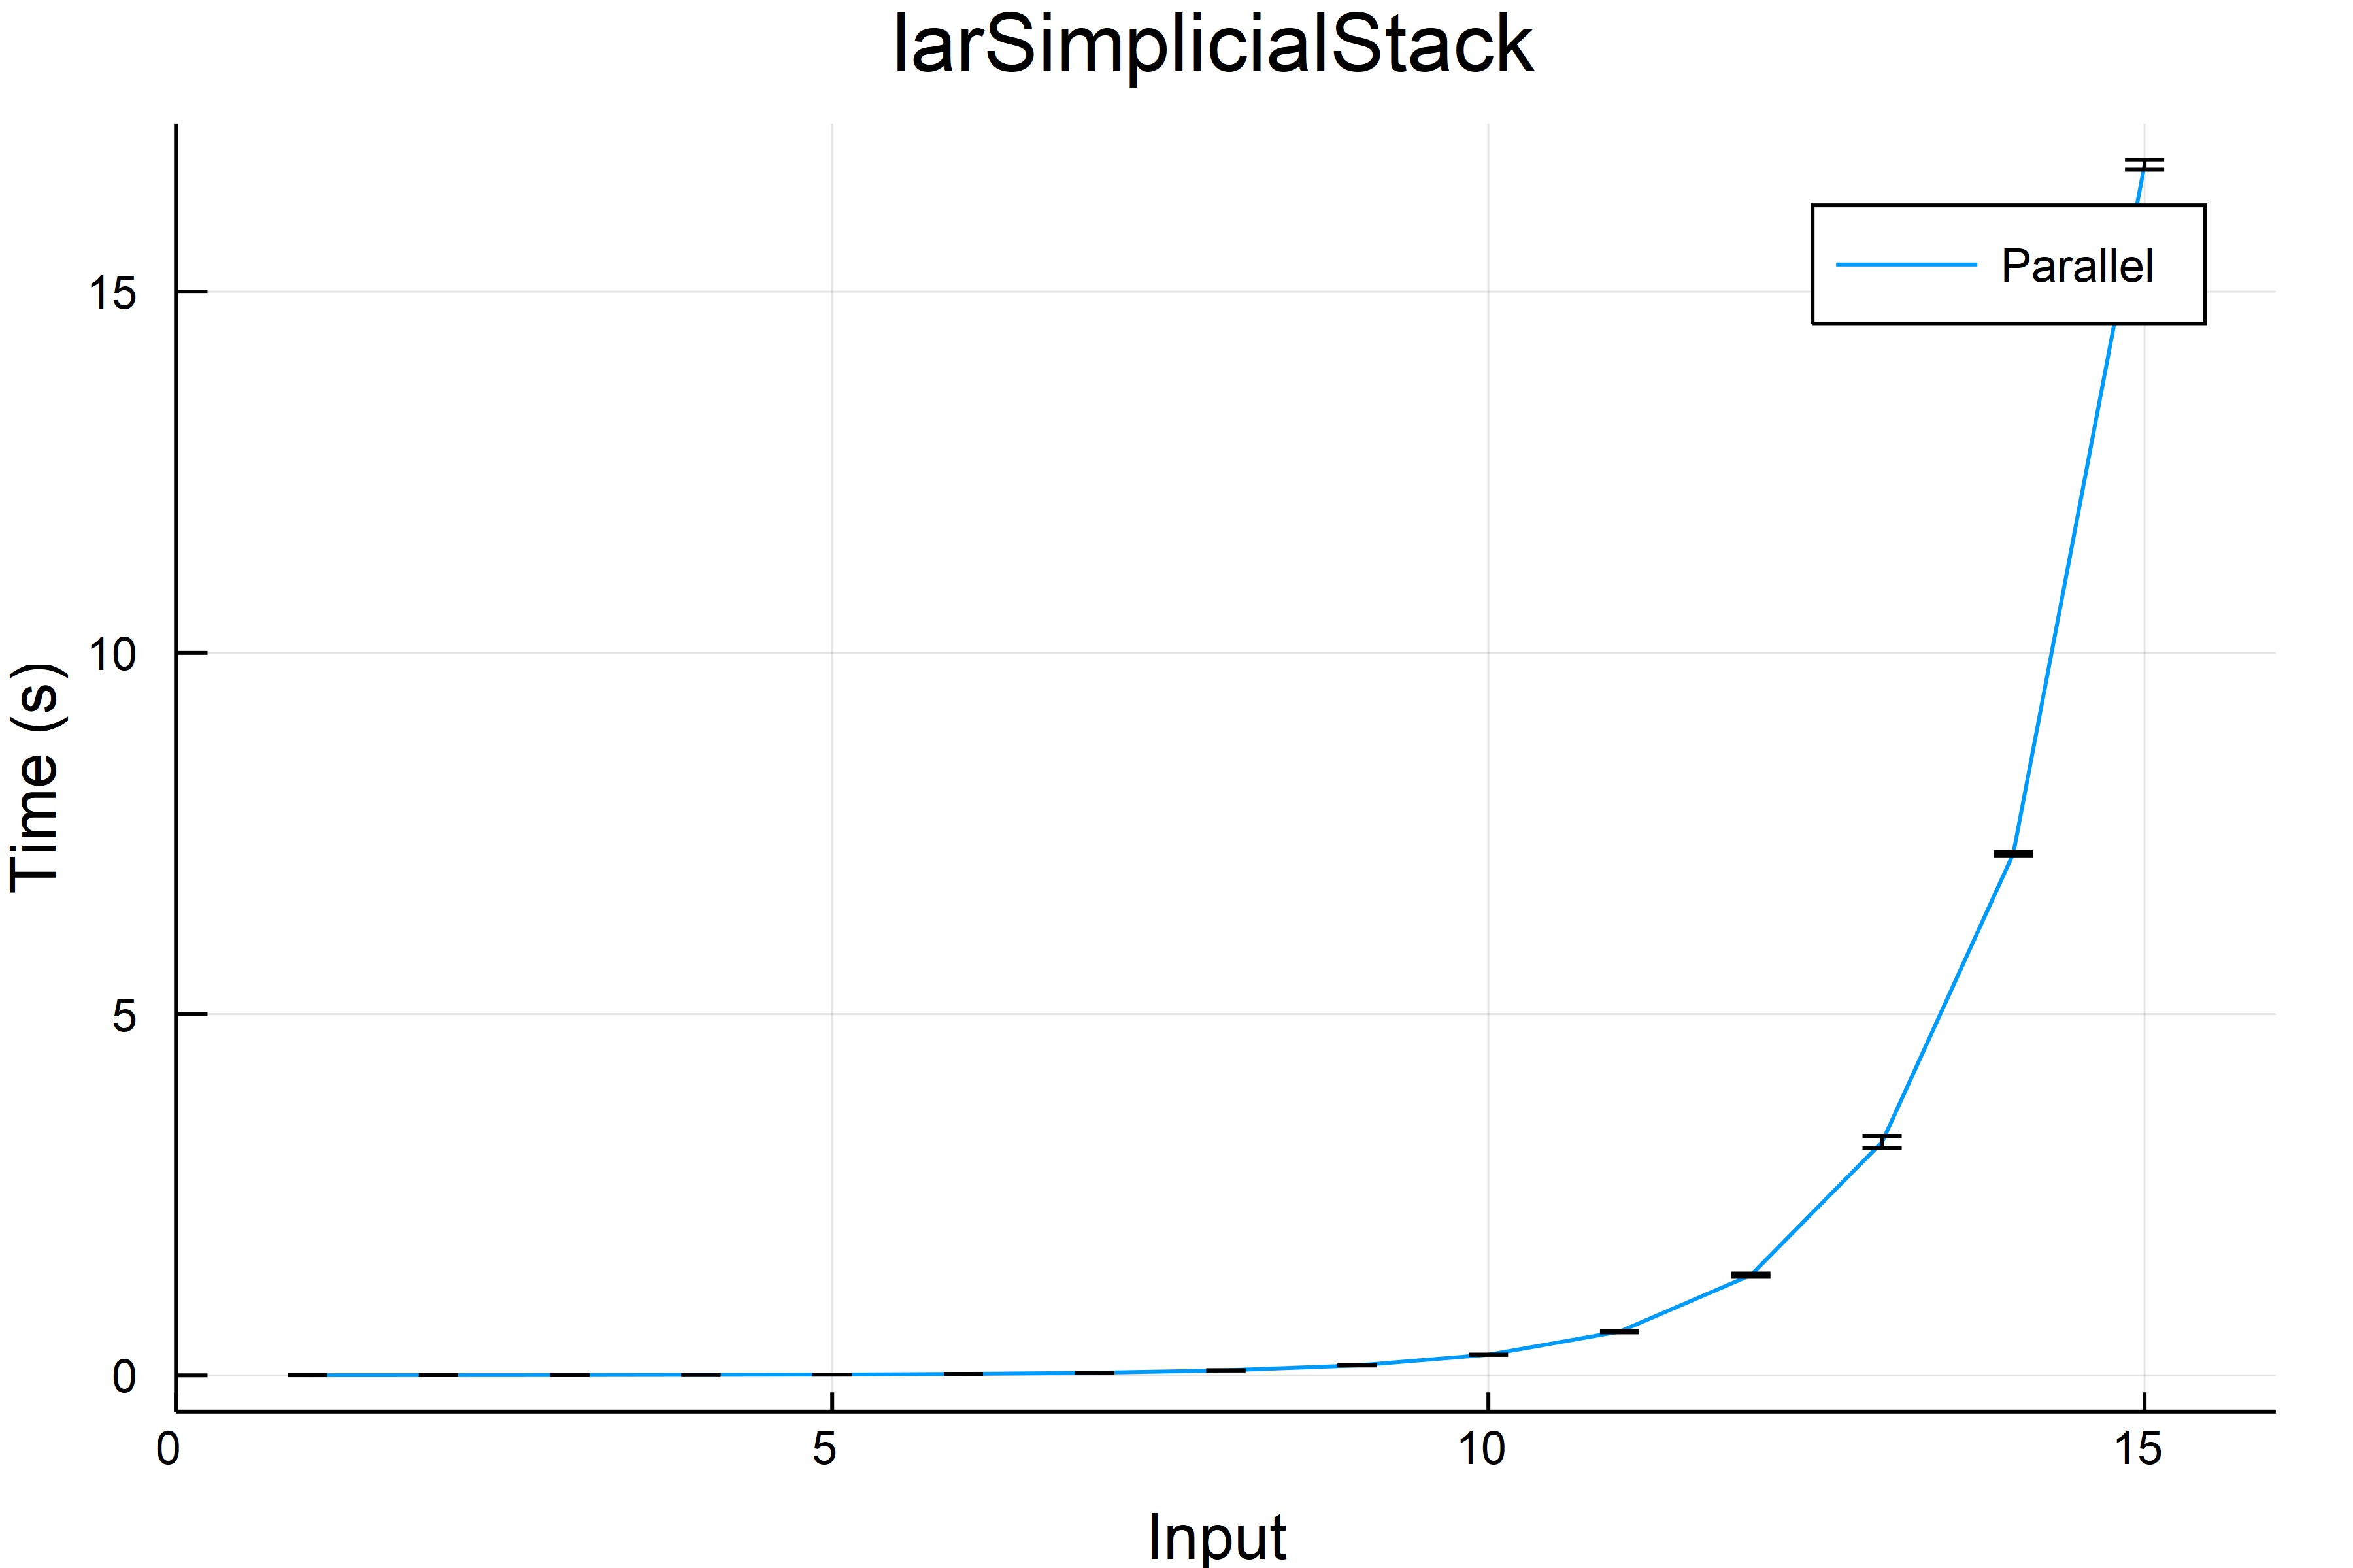
\includegraphics[scale=0.06]{larSimplicialStackPar.png}
\end{figure}

\paragraph{Compare}

\begin{flushleft}\small
\begin{list}{}{} \item
    \begin{Verbatim}[tabsize=4]
x=[xs,xp]
y=[ys,yp]
plot(x,y,yaxis="Time (s)",xlims = (0,length(datap)+1), xaxis="Input",
            title="larSimplicialStack",label=["Serial" "Parallel"],lw=1)
    \end{Verbatim}
\end{list}
\end{flushleft}   
\begin{figure}[h!]
\centering
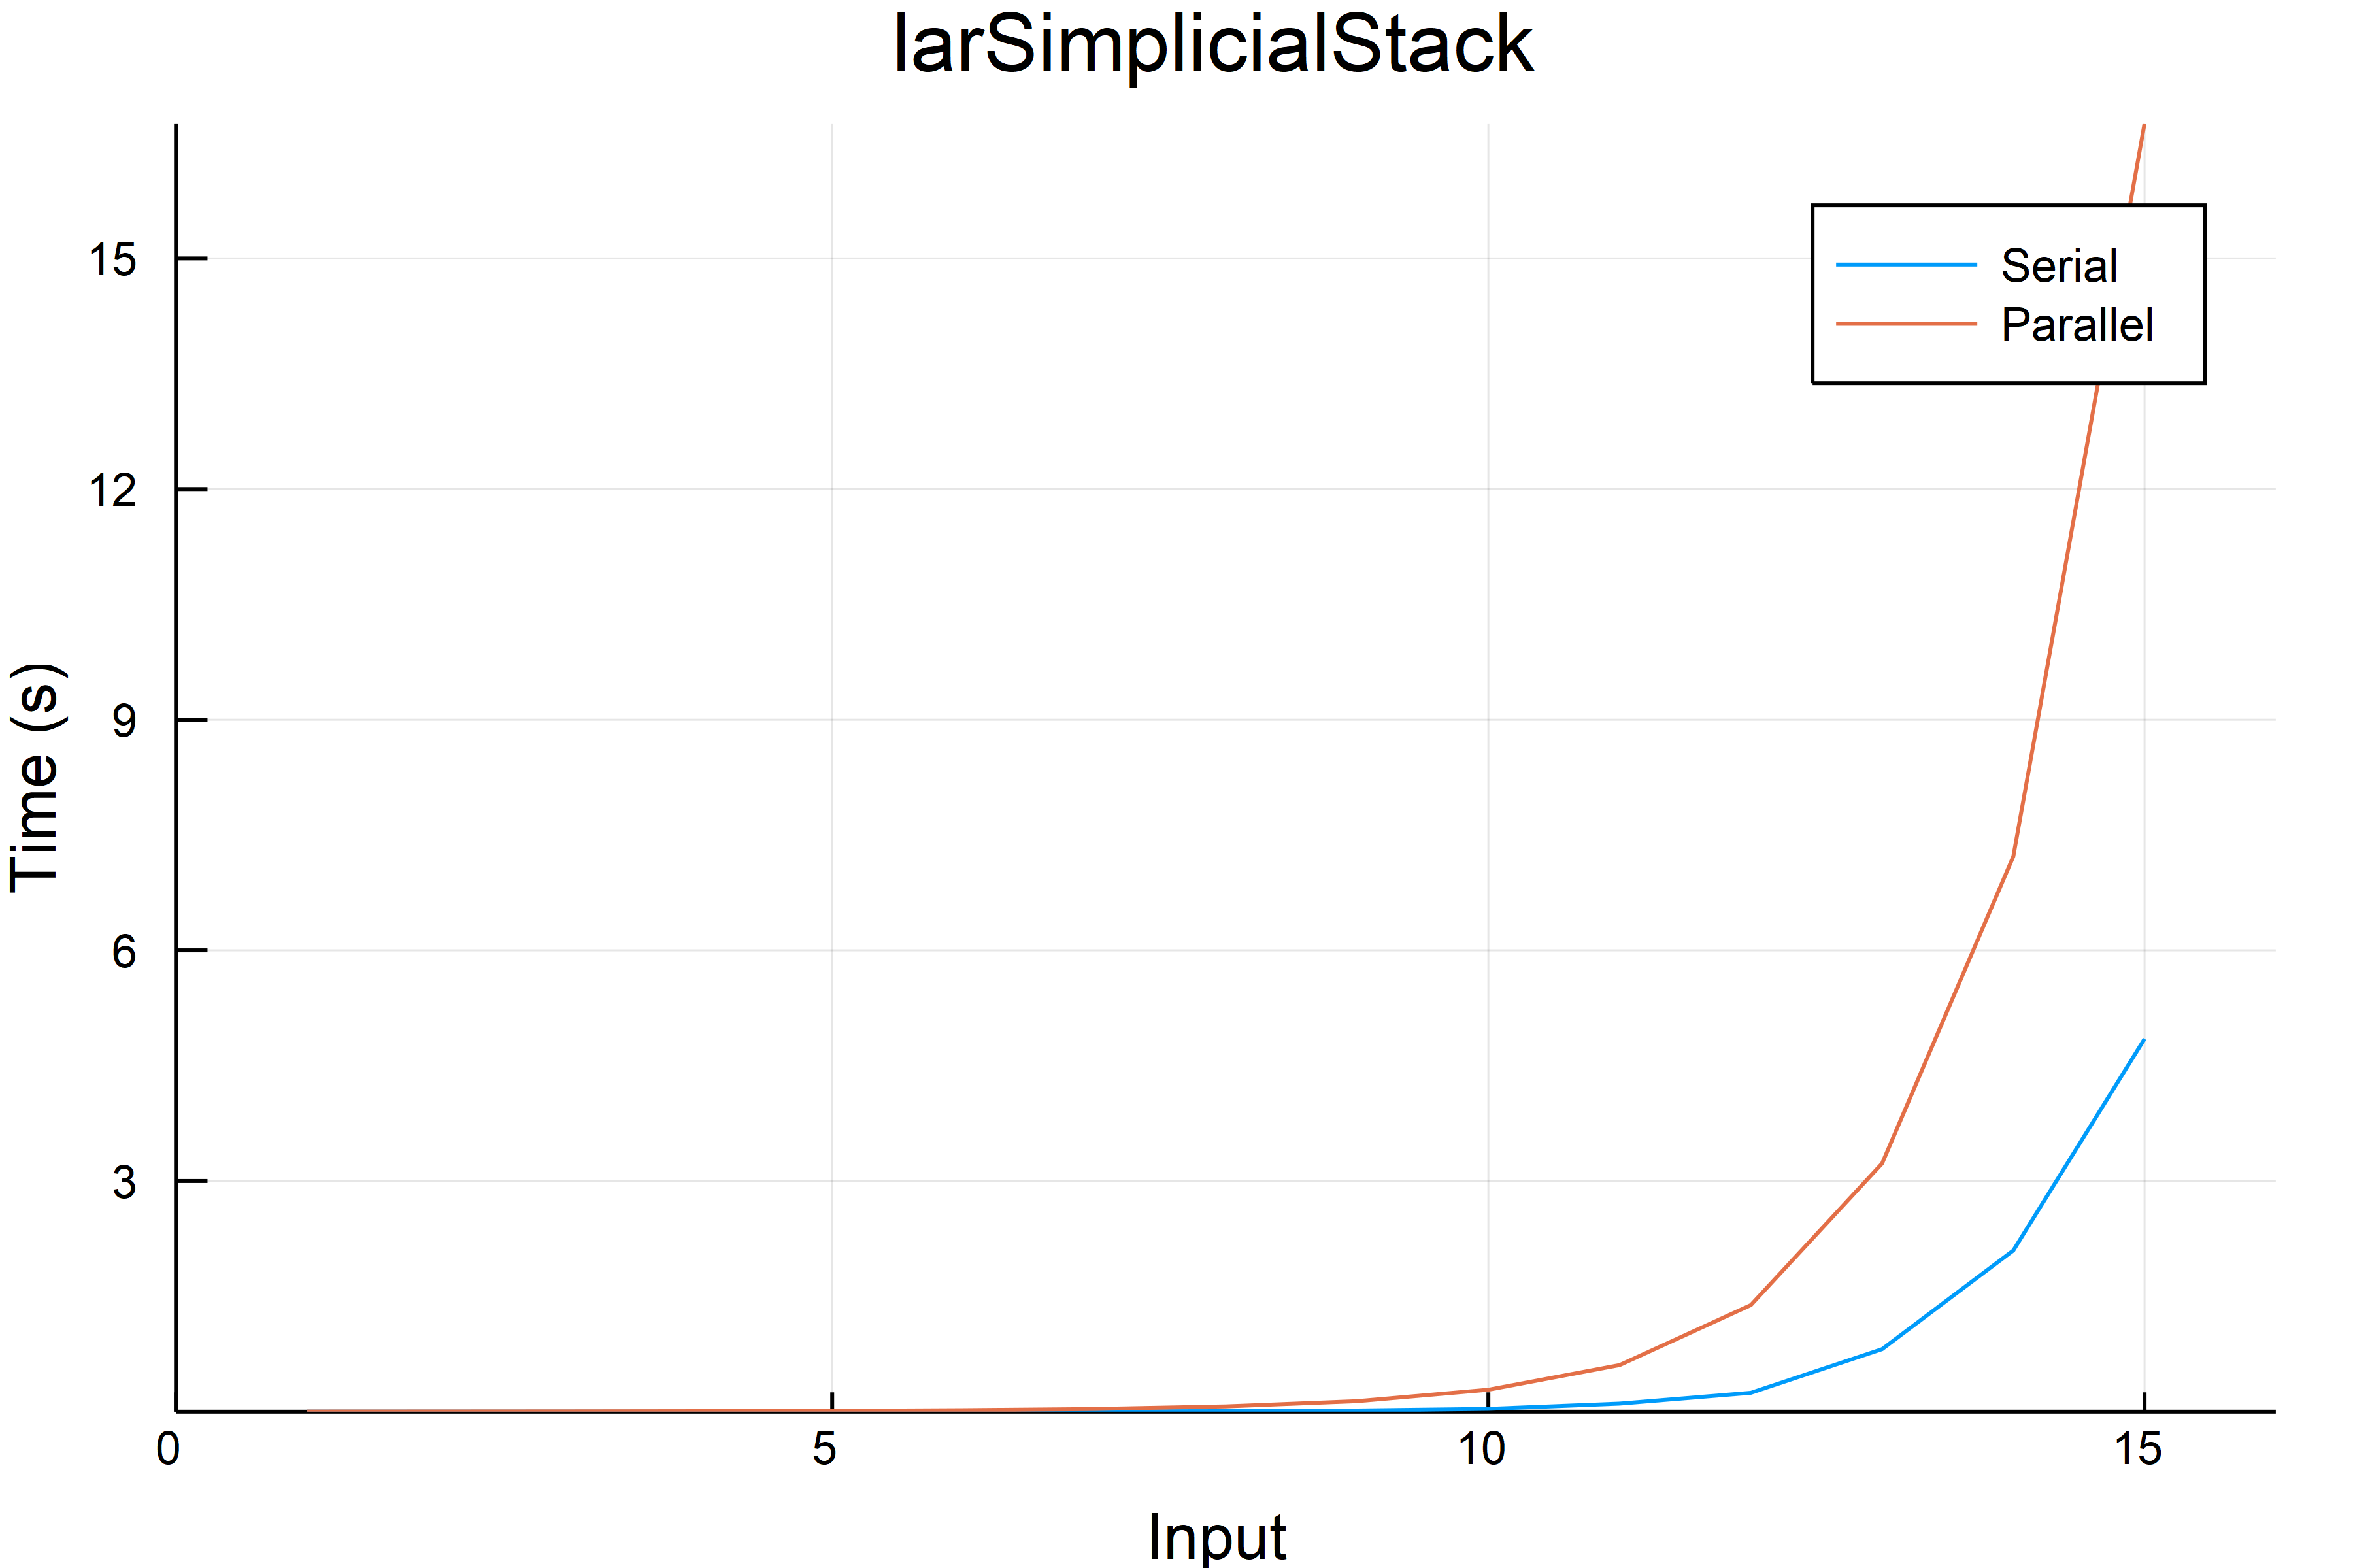
\includegraphics[scale=0.06]{larSimplicialStackCom.png}
\end{figure}

%-------------------------------------------------------------------------------
\subsection{larGridSkeleton:}

\subsubsection{Translation}
To be able to generate the various subsets of cells of a $d$-dimensional cuboidal grid skeleton, you needed of other results. 

First of all, the grid vertices are produced by the \texttt{larVertProd} function, via Cartesian product of
vertices of the $n$ 1-dimensional arguments, \texttt{cart} function implements Cartesian product with \texttt{product} in IterTools package.

The second-order utility \texttt{index2addr} function transforms a $shape$ list for a multidimensional array into a function that, when applied
to a multindex array, i.e. to a list of integers within the $shape$'s bounds, returns the integer address of the array component within the linear storage of the multidimensional array. 

\texttt{larCellProd} is usefull to construct Cartesian product of $0/1$-complexes.

The function \texttt{filterByOrder} is used to partition the binary strings, generated by \texttt{binaryRange} function, into $n + 1$
subsets, such that the bits into each string sum to the same number, ranging from $0$ to $n$ included, respectively.

Finally the second order function \texttt{larGridSkeleton} returns $d$-skeleton of cuboidal complex passed in input as $shape$. Furthermore, whereas the dimension $n$ of the embedding space is implicitly provided by the length of the $shape$ parameter, the intrinsic dimension $d$ of the skeleton to be produced must be given explicitly.
\vspace{2ex}
\begin{flushleft} \small
\begin{center}
\begin{tabular}{|p{16cm}|}
\hline
\cellcolor[gray]{.9}Python\\
\hline
\end{tabular}
\end{center}
\vspace{2ex}
\begin{list}{}{} \item
\begin{Verbatim}[tabsize=3]
def larVertProd(vertLists):
    return AA(CAT)(CART(vertLists))
	
def index2addr (shape):
    n = len(shape)
    shape = shape[1:]+[1]
    weights = [PROD(shape[k:]) for k in range(n)]
    def index2addr0 (multindex):
        return INNERPROD([multindex, weights])
    return index2addr0

def larCellProd(cellLists):
    shapes = [len(item) for item in cellLists]
    indices = CART([range(shape) for shape in shapes])
    jointCells = [CART([cells[k] 
        for k,cells in zip(index,cellLists)]) for index in indices]
    convert = index2addr([shape+1
        if (len(cellLists[k][0]) > 1) else shape for k,shape in enumerate(shapes)])
    return [AA(convert)(cell) 
                for cell in jointCells]

def binaryRange(n):
    return [('{0:0'+str(n)+'b}').format(k) for k in range(2**n)]

def filterByOrder(n):
    terms = [AA(int)(list(term)) for term in binaryRange(n)]
    return [[term for term in terms if sum(term) == k] for k in range(n+1)]
                        
def larGridSkeleton(shape):
    n = len(shape)
    def larGridSkeleton0(d):
        components = filterByOrder(n)[d]
        componentCellLists = [AA(APPLY)(zip(AA(larGrid)(shape),(component))) for component in components]
        return CAT([ larCellProd(cellLists) for cellLists in componentCellLists])
    return larGridSkeleton0                        
\end{Verbatim}
\end{list}
   \vspace{2ex}
\begin{center}
\begin{tabular}{|p{16cm}|}
\hline
\cellcolor[gray]{.9}Julia\\
\hline
\end{tabular}
\end{center}
\vspace{2ex}
\begin{list}{}{} \item
\begin{Verbatim}[tabsize=4]
function cart(args)
   return sort(collect(IterTools.product(args...)))
end

function larVertProd(vertLists)
   coords = [[x[1] for x in v] for v in cart(vertLists)]
   return sortcols(hcat(coords...))
end

function index2addr(shape::Array{Int64,1})
   index2addr(hcat(shape...))
end

function index2addr(shape::Array{Int64,2})
    n = length(shape)
    theShape = append!(shape[2:end],1)
    weights = [prod(theShape[k:end]) for k in range(1,n)]
    function index2addr0(multiIndex)
        return dot(collect(multiIndex), weights) + 1
    end
    return index2addr0
end

function larCellProd(cellLists)
   shapes = [length(item) for item in cellLists]
   subscripts = cart([collect(range(0,shape)) for shape in shapes])
   indices = hcat([collect(tuple) for tuple in subscripts]...)
   jointCells = Any[]
   for h in 1:size(indices,2)
      index = indices[:,h]
      cell = hcat(cart([cells[k+1] for (k,cells) in zip(index,cellLists)])...)
      append!(jointCells,[cell])
   end
   convertIt = index2addr([(length(cellLists[k][1]) > 1)? shape+1 :
                                            shape for (k,shape) in enumerate(shapes)])
   [vcat(map(convertIt, jointCells[j])...) for j in 1:size(jointCells,1)]
end

function binaryRange(n)
   return [bin(k,n) for k in 0:2^n-1]
end

function filterByOrder(n)
   terms = [[parse(Int8,bit) for bit in convert(Array{Char,1},term)] for term in binaryRange(n)]
   return [[term for term in terms if sum(term) == k] for k in 0:n]
end

function larGridSkeleton(shape)
    n = length(shape)
    function larGridSkeleton0(d)
        components = filterByOrder(n)[d+1]
        mymap(arr) = [arr[:,k]  for k in 1:size(arr,2)] 
        componentCellLists = [[mymap(f(x)) for (f,x) in zip( [larGrid(dim) for dim in shape],component)]
                                                                            for component in components]
        out = [larCellProd(cellLists) for cellLists in componentCellLists]
        return vcat(out...)
    end
    return larGridSkeleton0
end
\end{Verbatim}
\end{list}
\end{flushleft}

\vspace{2ex}
\subsubsection{Vectorize}
To vectorize \texttt{larCellProd} on elements of range, it's created second order function \texttt{larCellProd0}, that takes in input as first argument $indices$ and $cellLists$, and as second argument an \texttt{int} $h$. 
\vspace{1ex}
\begin{flushleft} \small
\begin{center}
\begin{tabular}{|p{16cm}|}
\hline
\cellcolor[gray]{.9}Vectorized code\\
\hline
\end{tabular}
\end{center}
\vspace{2ex}
\begin{list}{}{} \item
   \begin{Verbatim}[tabsize=4]
function larCellProd0(indices,cellLists)
	function larCellProd1(h)
		index = indices[:,h]
		cell = hcat(cart([cells[k+1] for (k,cells) in zip(index,cellLists)])...)	
		return cell
	end
	return larCellProd1
end
	
function vlarCellProd(cellLists)
	shapes = length.(cellLists)
	subscripts = cart(collect(range.(0,shapes)))
	indices = hcat(collect.(subscripts)...)
	jointCells = larCellProd0(indices,cellLists).( range(1,size(indices,2)))
	convertIt = index2addr([(length(cellLists[k][1]) > 1)? shape+1 : shape 
					for (k,shape) in enumerate(shapes)])
	[vcat(convertIt.(jointCells[j])...) for j in 1:size(jointCells,1)]
end

function vbinaryRange(n)
	return bin.(range(0,2^n),n) 
end

function vlarImageVerts(shape)
	vertLists = vertexDomain.(shape+1) 
	vertGrid = larVertProd(vertLists)
	return vertGrid
end

function vfilterByOrder(n)
	terms = [[parse(Int8,bit) for bit in convert(Array{Char,1},term)] 
							for term in vbinaryRange(n)]
	return [[term for term in terms if sum(term) == k] for k in 0:n]
end

function vlarGridSkeleton(shape)
    n = length(shape)
    function larGridSkeleton0(d)
        components = filterByOrder(n)[d+1]
        mymap(arr) = [arr[:,k] for k in 1:size(arr,2)]
        componentCellLists = [[mymap(f(x)) 
				for (f,x) in zip(larGrid.(shape),component)]
					for component in components]
        out = vlarCellProd.(componentCellLists)
        return vcat(out...)
    end
    return larGridSkeleton0
end
   \end{Verbatim}
\end{list}


\vspace{2ex}
\subsubsection{Parallel computing}
To parallel \texttt{larGridSkeleton}, the only function in which to replace a loop \texttt{for} with a \texttt{@parallel for} is \texttt{larCellProd}, so the other functions have to be declared on all processes with macro \texttt{@everywhere}. 
\vspace{1ex}
\begin{center}
\begin{tabular}{|p{16cm}|}
\hline
\cellcolor[gray]{.9}Parallel\\
\hline
\end{tabular}
\end{center}
\vspace{2ex}
\begin{list}{}{} \item
   \begin{Verbatim}[tabsize=4]
@everywhere function cart(args)
   return sort(collect(IterTools.product(args...)))
end

@everywhere function larVertProd(vertLists)
   coords = [[x[1] for x in v] for v in cart(vertLists)]
   return sortcols(hcat(coords...))
end

@everywhere function index2addr(shape::Array{Int64,1})
   index2addr(hcat(shape...))
end

@everywhere function index2addr(shape::Array{Int64,2})
    n = length(shape)
    theShape = append!(shape[2:end],1)
    weights = [prod(theShape[k:end]) for k in range(1,n)]
    function index2addr0(multiIndex)
        return dot(collect(multiIndex), weights) + 1
    end
    return index2addr0
end

@everywhere function plarCellProd(cellLists)
	shapes = [length(item) for item in cellLists]
	subscripts = cart([collect(range(0,shape)) for shape in shapes])
	indices = hcat([collect(tuple) for tuple in subscripts]...)
	jointCells = Any[]
	jointCells = @parallel (append!) for h in 1:size(indices,2)
		index = indices[:,h]
		cell = [hcat(cart([cells[k+1] for (k,cells) in zip(index,cellLists)])...)]
	end
	convertIt = index2addr([ (length(cellLists[k][1]) > 1)? shape+1 : shape 
		for (k,shape) in enumerate(shapes) ])     
	[vcat(pmap(convertIt, jointCells[j])...) for j in 1:size(jointCells,1)]
end

@everywhere function binaryRange(n)
   return [bin(k,n) for k in 0:2^n-1]
end

@everywhere function filterByOrder(n)
   terms = [[parse(Int8,bit) for bit in convert(Array{Char,1},term)]
		for term in binaryRange(n)]
   return [[term for term in terms if sum(term) == k] for k in 0:n]
end

@everywhere function plarGridSkeleton(shape)
    n = length(shape)
    function larGridSkeleton0(d)
        components = filterByOrder(n)[d+1]
        mymap(arr) = [arr[:,k] for k in 1:size(arr,2)]
        componentCellLists = [[mymap(f(x)) for (f,x) in zip([larGrid(dim) 
			for dim in shape], component)] for component in components]
		out = pmap(plarCellProd,componentCellLists)
        return vcat(out...)
    end
    return larGridSkeleton0
end   
   \end{Verbatim}
\end{list}
\footnotesize\addtolength{\baselineskip}{-1ex}
\end{flushleft}
\vspace{2ex}

\subsubsection{Test}
\begin{center}
\begin{tabular}{|p{16cm}|}
\hline
\cellcolor[gray]{.9}Test\\
\hline
\end{tabular}
\end{center}


\begin{flushleft}\small
\begin{list}{}{} \item
\begin{Verbatim}[tabsize=4]
@testset "Index2addr Tests" begin
		@testset "shape 1D" begin
			@test index2addr([10])([0])==1
			@test index2addr([10])([9])==10
			@test [index2addr([10])([index]) for index in collect(0:9)]==collect(1:10)
		end

		@testset "shape 3d" begin
		aaa = cart([collect(0:3),collect(0:2),collect(0:1)])
		bbb = cart([[0;1;2],[0;1],[0;1]])
		ccc = cart([[0;1],[0;1],[0;1;2]])
			@test index2addr([3,2,1])([0,0,0]) == 1
			@test [ index2addr([4,3,2])(index) for index in aaa ] == collect(1:24)
			@test [index2addr([3,2,2])(index) for index in bbb ] == collect(1:12)
			@test [index2addr([2,2,3])(index) for index in ccc ] == collect(1:12)
		end
end

@testset "BinaryRange Tests" begin
		@test binaryRange(1)==["0";"1"]
		@test binaryRange(2)==["00","01","10","11"]
		@test binaryRange(3)==["000","001","010","011","100","101","110","111"]
end

@testset "LarVertProd Tests" begin
		@testset "LarVertProd 1D" begin
			shape = [3]
			vertLists = [vertexDomain(k+1) for k in shape]
			@test typeof(larVertProd(vertLists))==Array{Int64,2}
			@test size(larVertProd(vertLists))==(1, 4)
			@test larVertProd(vertLists)[:,1]==[0]
			@test larVertProd(vertLists)[:,4]==[3]
		end

		@testset "LarVertProd 2D" begin
			shape = [3,2]
			vertLists = [vertexDomain(k+1) for k in shape]
			@test typeof(larVertProd(vertLists))==Array{Int64,2}
			@test size(larVertProd(vertLists))==(2, 12)
			@test larVertProd(vertLists)[:,1]==[0;0]
			@test larVertProd(vertLists)[:,12]==[3;2]
		end

		@testset "LarVertProd 3D" begin
			shape = [3,2,1]
			vertLists = [vertexDomain(k+1) for k in shape]
			@test typeof(larVertProd(vertLists))==Array{Int64,2}
			@test size(larVertProd(vertLists))==(3, 24)
			@test larVertProd(vertLists)[:,1]==[0;0;0]
			@test larVertProd(vertLists)[:,24]==[3;2;1]
		end
end

@testset "FilterByOrder Tests" begin
		term = "000"
		bit = '0'
		theTerm = convert(Array{Char,1},term)
		@test typeof(theTerm) == Array{Char,1}
		@test parse(Int8,bit) == 0
		@test [parse(Int8,bit) for bit in theTerm] == zeros(3)
		out = hcat([[parse(Int8,bit) for bit in term] for term in binaryRange(3)]...)
		@test typeof(out) == Array{Int8,2}
		@test size(out) == (3,8)
		@test repr(out) == "Int8[0 0 0 0 1 1 1 1; 0 0 1 1 0 0 1 1; 0 1 0 1 0 1 0 1]"
end
	
@testset "larGridSkeleton Tests" begin
		@test length(larGridSkeleton([1,1,1])(0)) == 8
		@test length(larGridSkeleton([1,1,1])(1)) == 12
		@test length(larGridSkeleton([1,1,1])(2)) == 6
		@test length(larGridSkeleton([1,1,1])(3)) == 1
end

@testset "vBinaryRange Tests" begin
		    @test vbinaryRange(1)==["0";"1"]
		    @test vbinaryRange(2)==["00","01","10","11"]
		    @test vbinaryRange(3)==["000","001","010","011","100","101","110","111"]
	    end

	    @testset "vfilterByOrder Tests" begin
		    @testset  "$n" for n in 1:4
			    data = [vfilterByOrder(n)[k] for (k,el) in enumerate(vfilterByOrder(n))]
			    @test sum(map(length,data)) == 2^n
		    end

		    @testset "$n,$k" for n in 1:4, k in 0:n
			    @test length(vfilterByOrder(n)[k+1]) == binomial(n,k)
		    end 
end

@testset "vlarGridSkeleton Tests" begin
		    @test length(vlarGridSkeleton([1,1,1])(0)) == 8
		    @test length(vlarGridSkeleton([1,1,1])(1)) == 12
		    @test length(vlarGridSkeleton([1,1,1])(2)) == 6
		    @test length(vlarGridSkeleton([1,1,1])(3)) == 1
end
	    
@testset "plarGridSkeleton Tests" begin
    		@test length(plarGridSkeleton([1,1,1])(0)) == 8
    		@test length(plarGridSkeleton([1,1,1])(1)) == 12
    		@test length(plarGridSkeleton([1,1,1])(2)) == 6
    		@test length(plarGridSkeleton([1,1,1])(3)) == 1
end
\end{Verbatim}
\end{list}
\end{flushleft}
\subsubsection{Execution time}
\begin{center}
\begin{tabular}{|p{16cm}|}
\hline
\cellcolor[gray]{.9}Execution time\\
\hline
\end{tabular}
\end{center}


\paragraph{Serial}
\begin{flushleft}\small
\begin{list}{}{} \item
    \begin{Verbatim}[tabsize=4]
datas=[Time(N,larGridSkeleton([j,j,j]),1) for j in range(1,10)]

xs=[1:length(datas);]
ys=mean.(datas)
yerrs=std.(datas)/sqrt(N)

plot(xs,ys,yaxis="Time (s)",xlims = (0,length(datas)+1), yerr = yerrs, xaxis="Input", 
                                            title="larGridSkeleton",label=["Serial"],lw=1)
    \end{Verbatim}
\end{list}
\end{flushleft}  

\paragraph{Vectorize}
\begin{flushleft}\small
\begin{list}{}{} \item
    \begin{Verbatim}[tabsize=4]
datav=[Time(N,vlarGridSkeleton([j,j,j]),1) for j in range(1,10)]

xv=[1:length(datav);]
yv=mean.(datav)
yerrv=std.(datav)/sqrt(N)

plot(xv,yv,yaxis="Time (s)",xlims = (0,length(datav)+1), yerr = yerrv, xaxis="Input", 
                                        title="larGridSkeleton",label=["Vectorize"],lw=1)
    \end{Verbatim}
\end{list}
\end{flushleft}
\begin{figure}[h!]
\centering
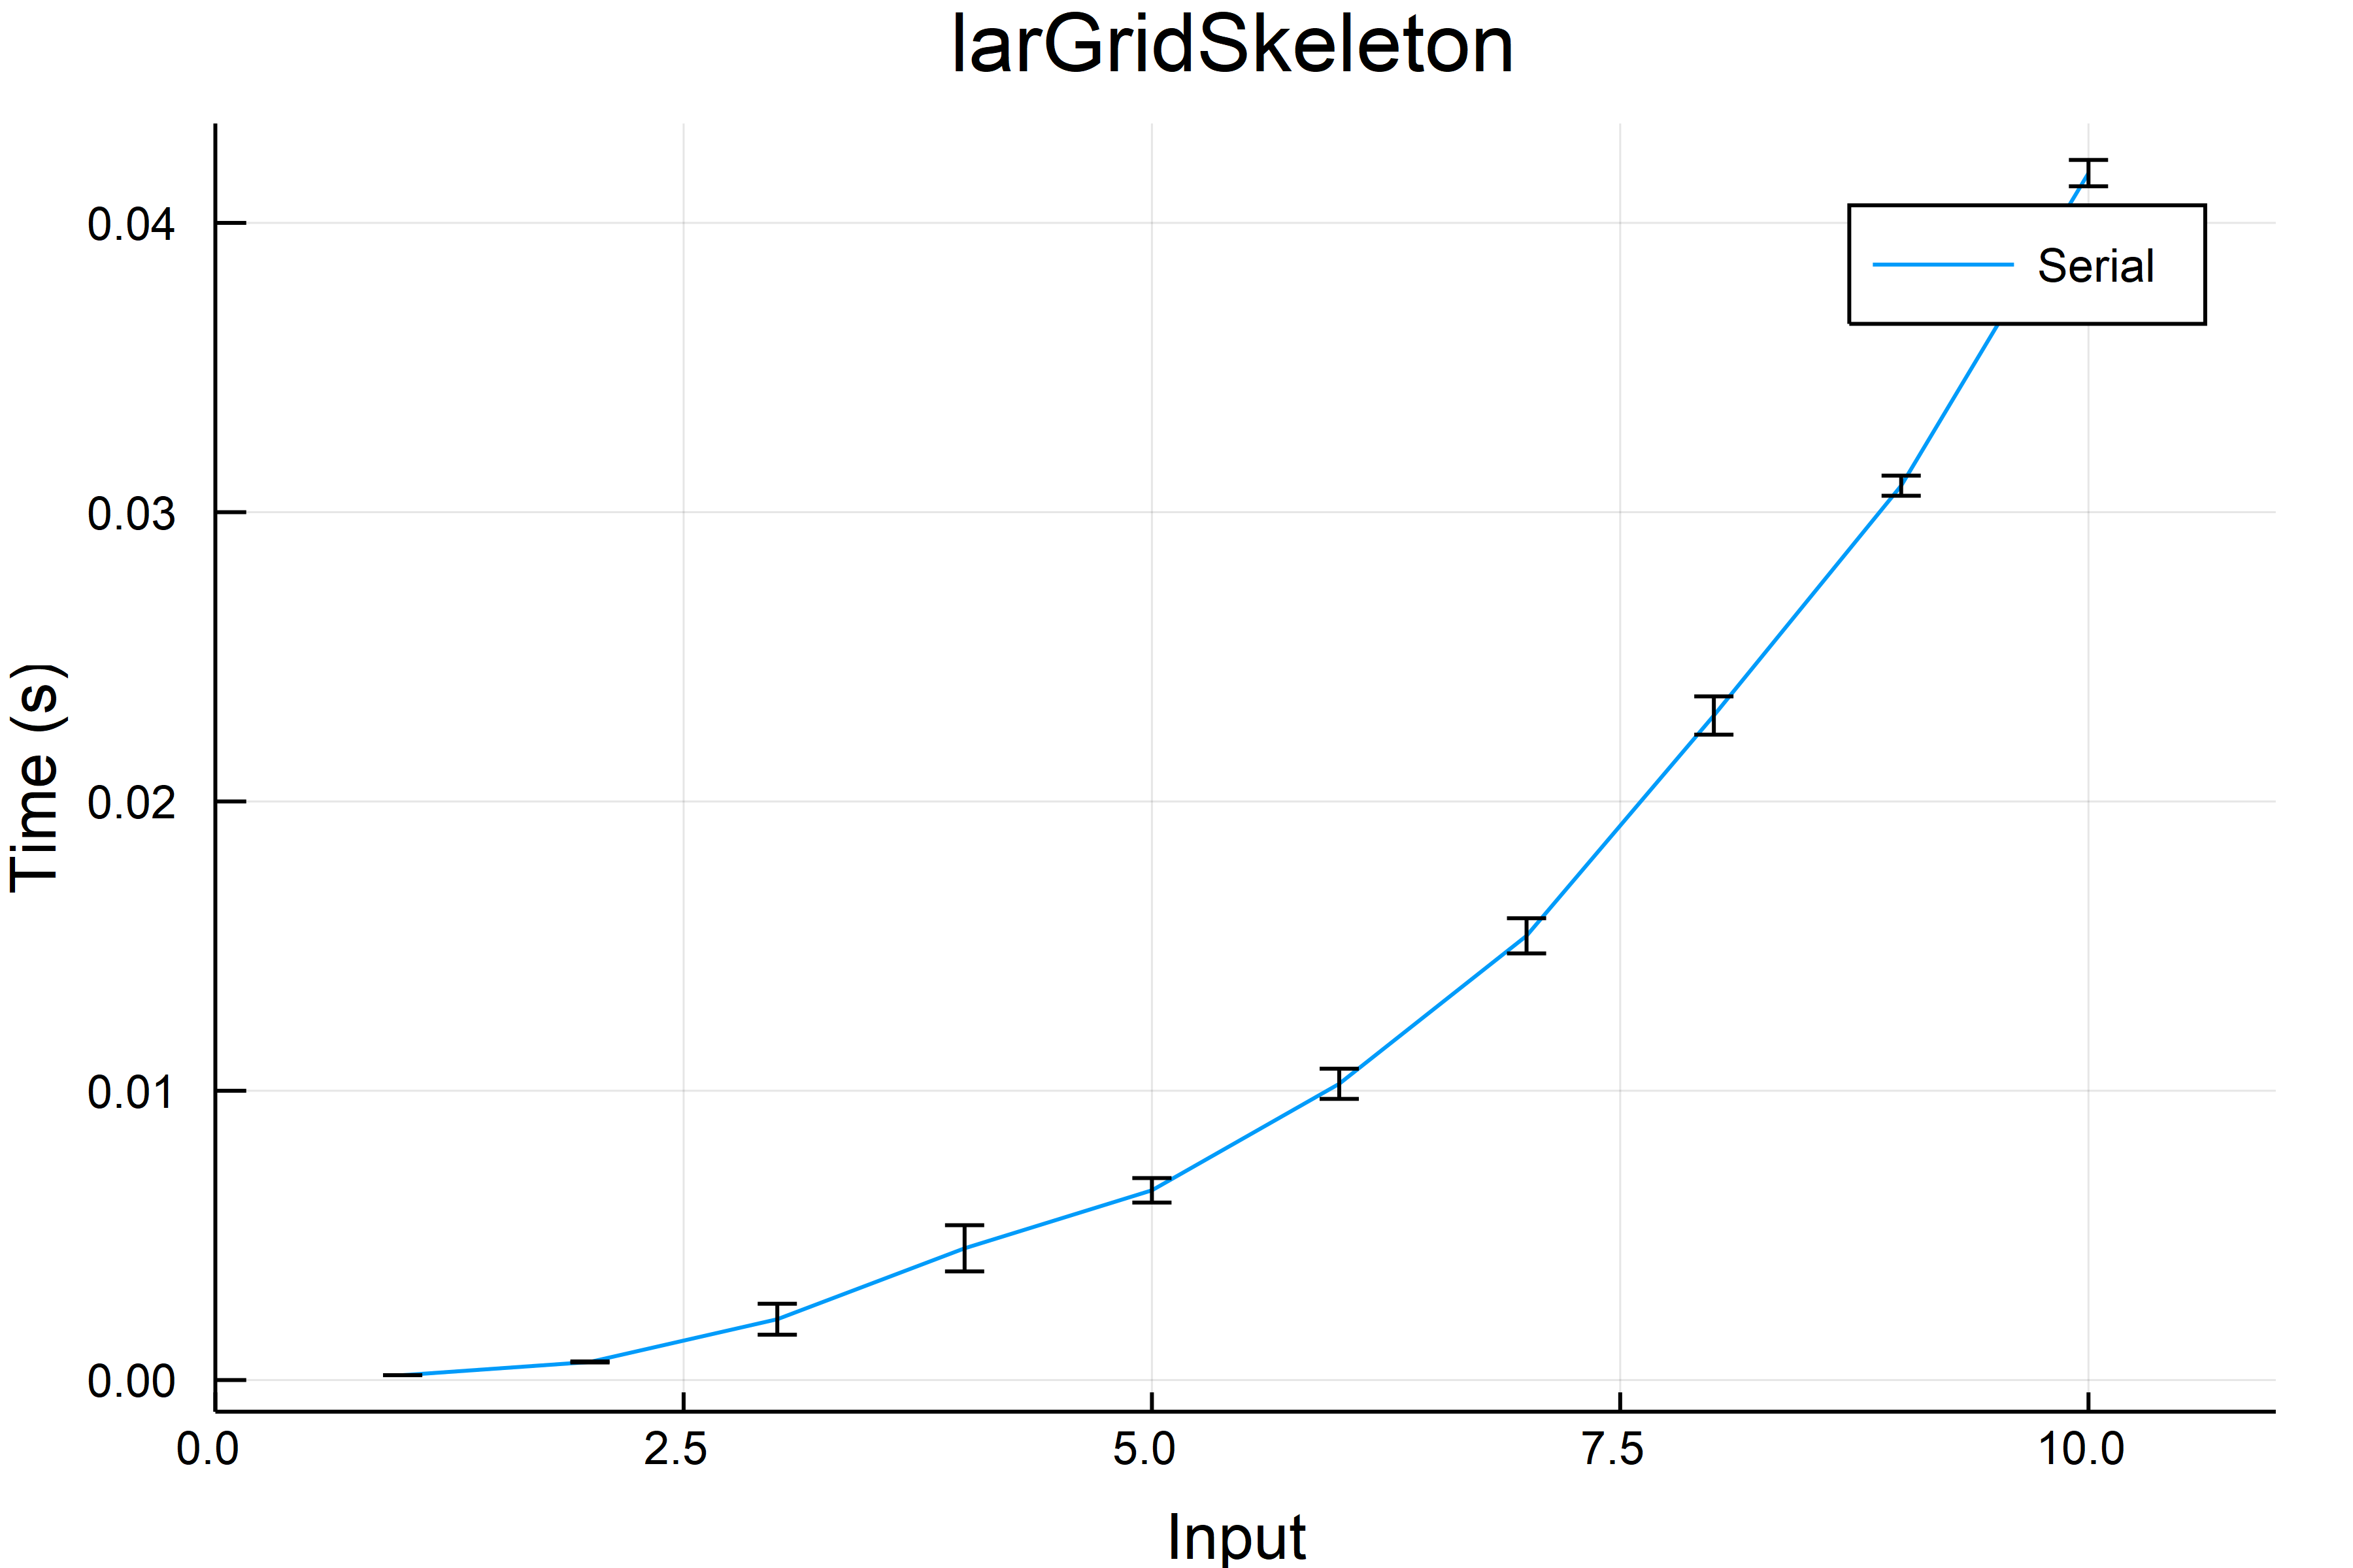
\includegraphics[scale=0.06]{larGridSkeletonSer.png}
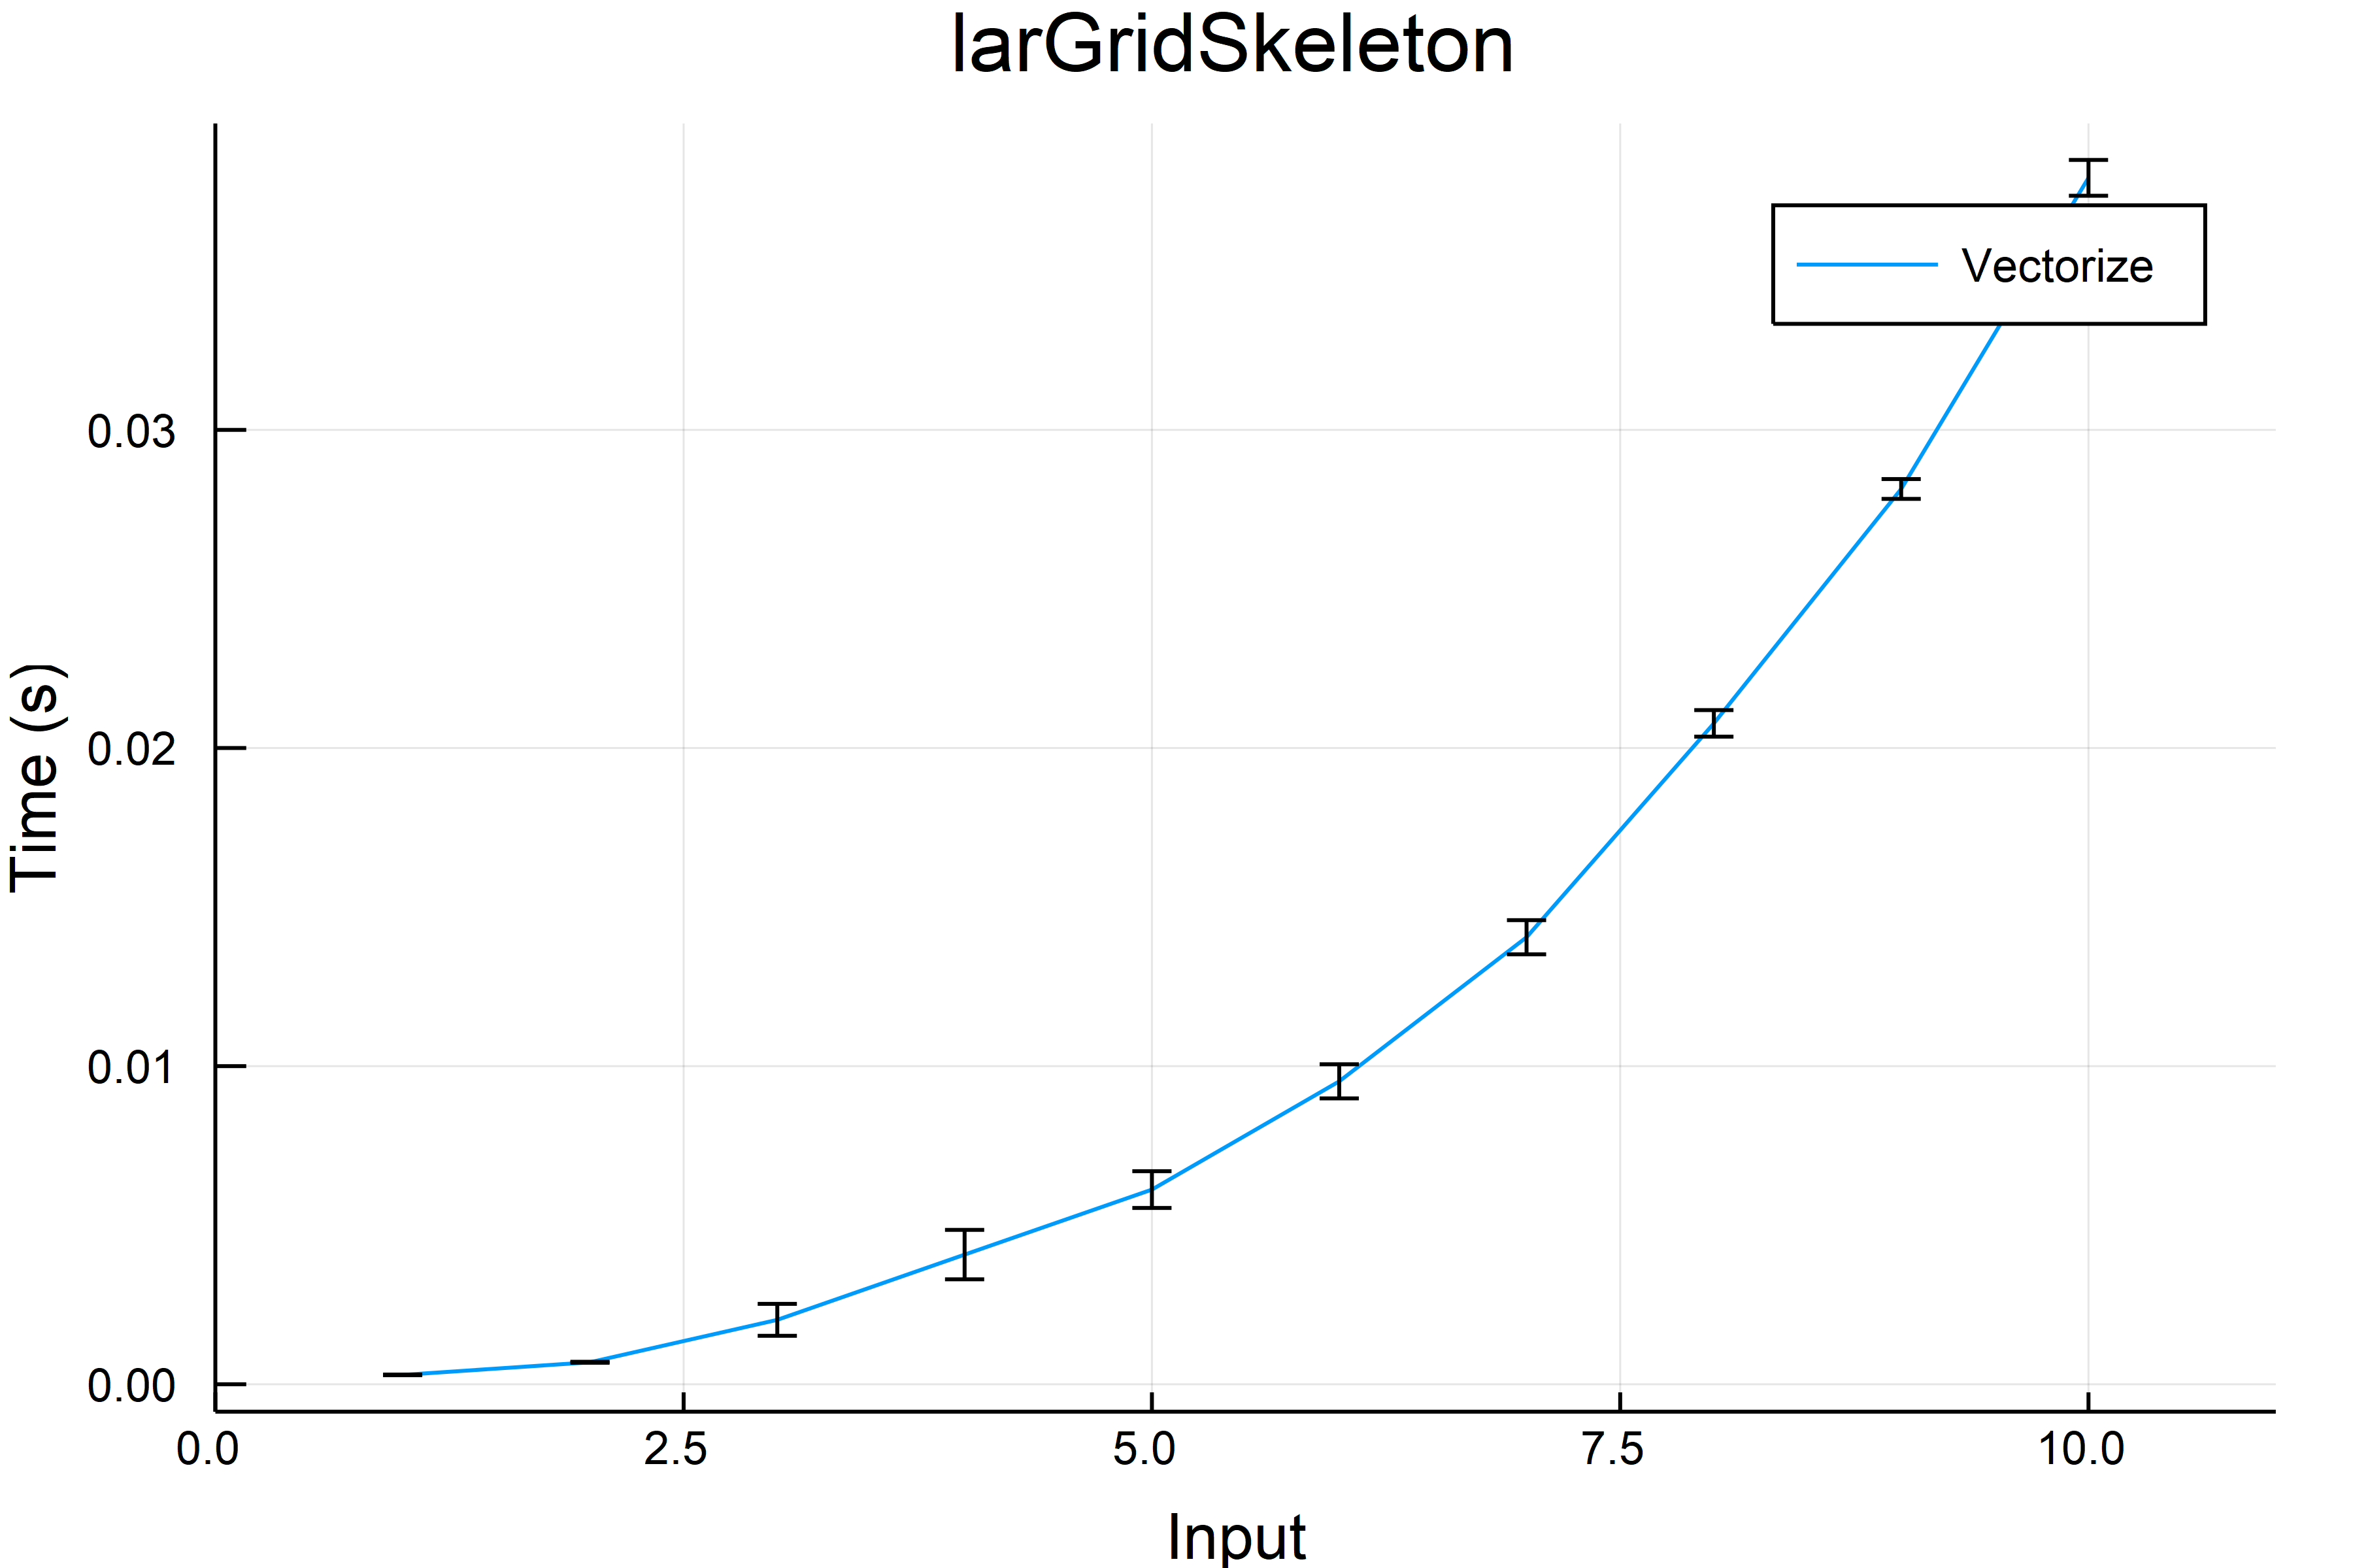
\includegraphics[scale=0.06]{larGridSkeletonVec.png}
\end{figure}

\paragraph{Compare}
\begin{flushleft}\small
\begin{list}{}{} \item
    \begin{Verbatim}[tabsize=4]
x=[xs,xv]
y=[ys,yv]

plot(x,y,yaxis="Time (s)",xlims = (0,length(datap)+1), xaxis="Input", title="larGridSkeleton",
                                                                label=["Serial" "Vectorize"],lw=1)
    \end{Verbatim}
\end{list}
\end{flushleft}   
\begin{figure}[h!]
\centering
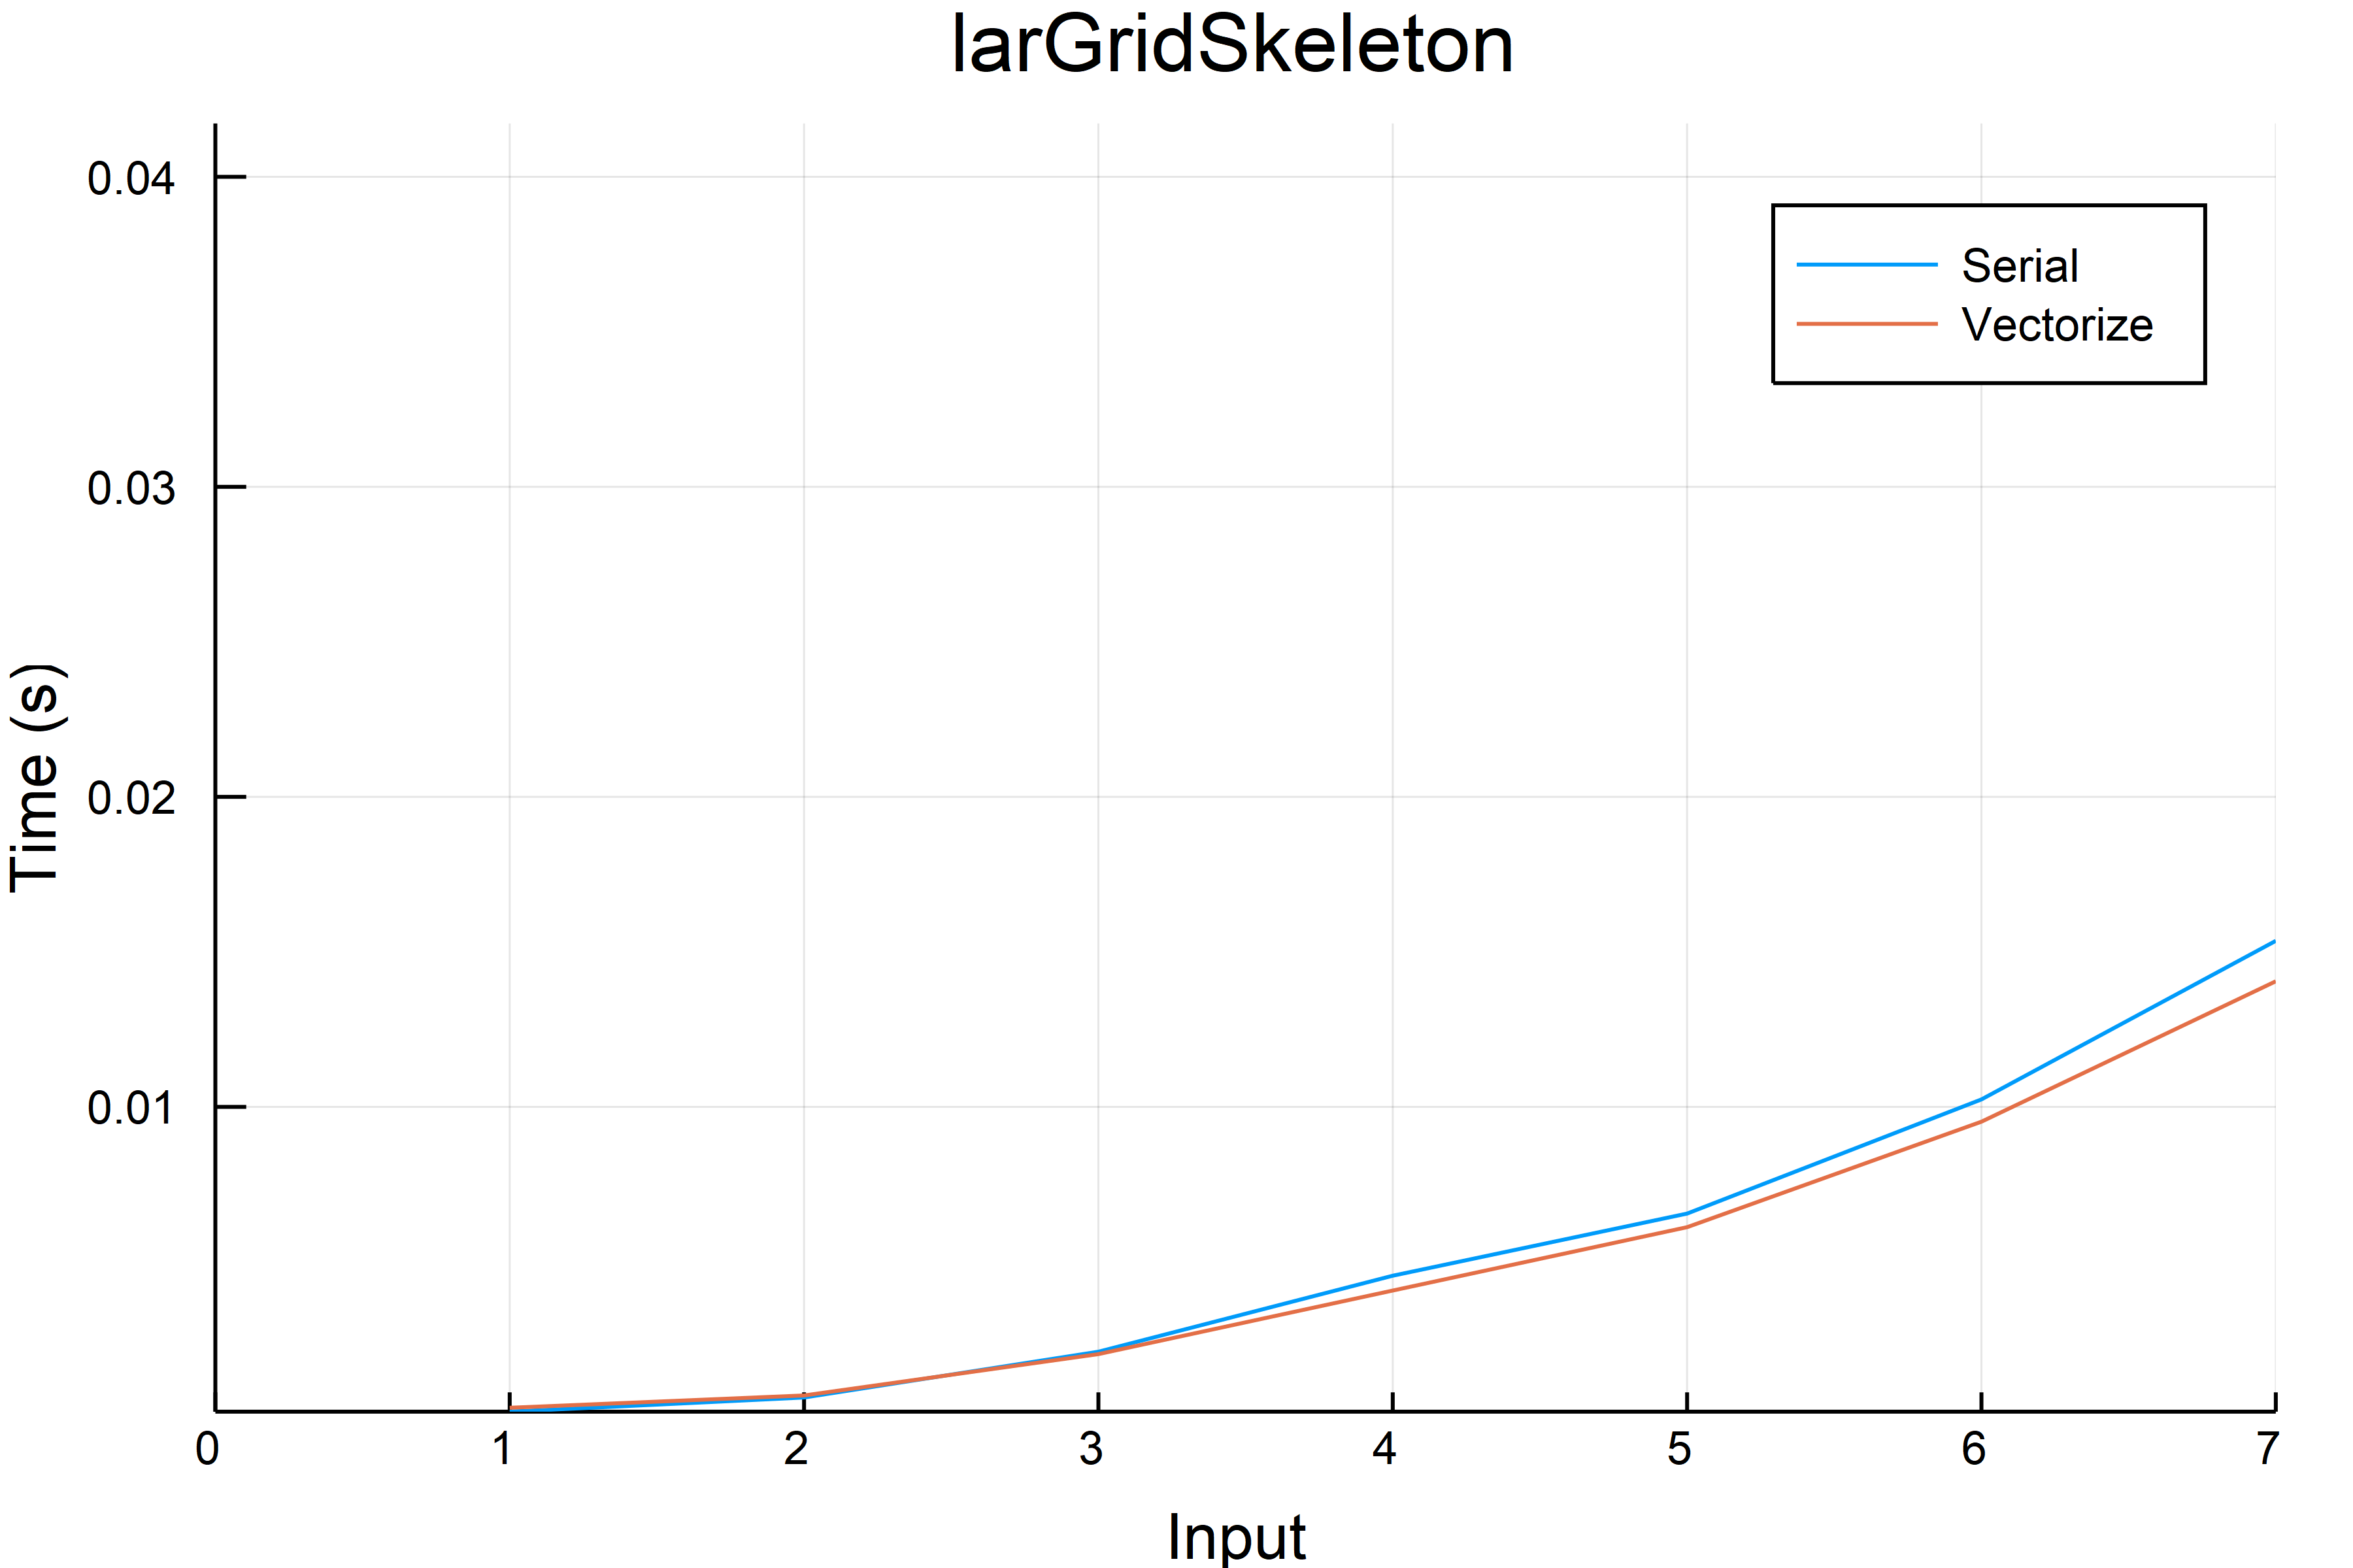
\includegraphics[scale=0.06]{larGridSkeletonCom1.png}
\end{figure}

\paragraph{Parallel}
\begin{flushleft}\small
\begin{list}{}{} \item
    \begin{Verbatim}[tabsize=4]
datap=[Time(N,plarGridSkeleton([j,j,j]),1) for j in range(1,6)]

xp=[1:length(datap);]
yp=mean.(datap)
yerrp=std.(datap)/sqrt(N)

plot(xp,yp,yaxis="Time (s)",xlims = (0,length(datap)+1), yerr = yerrp, xaxis="Input", 
                                            title="larGridSkeleton",label=["Parallel"],lw=1)
    \end{Verbatim}
\end{list}
\end{flushleft}  
\begin{figure}[h!]
\centering
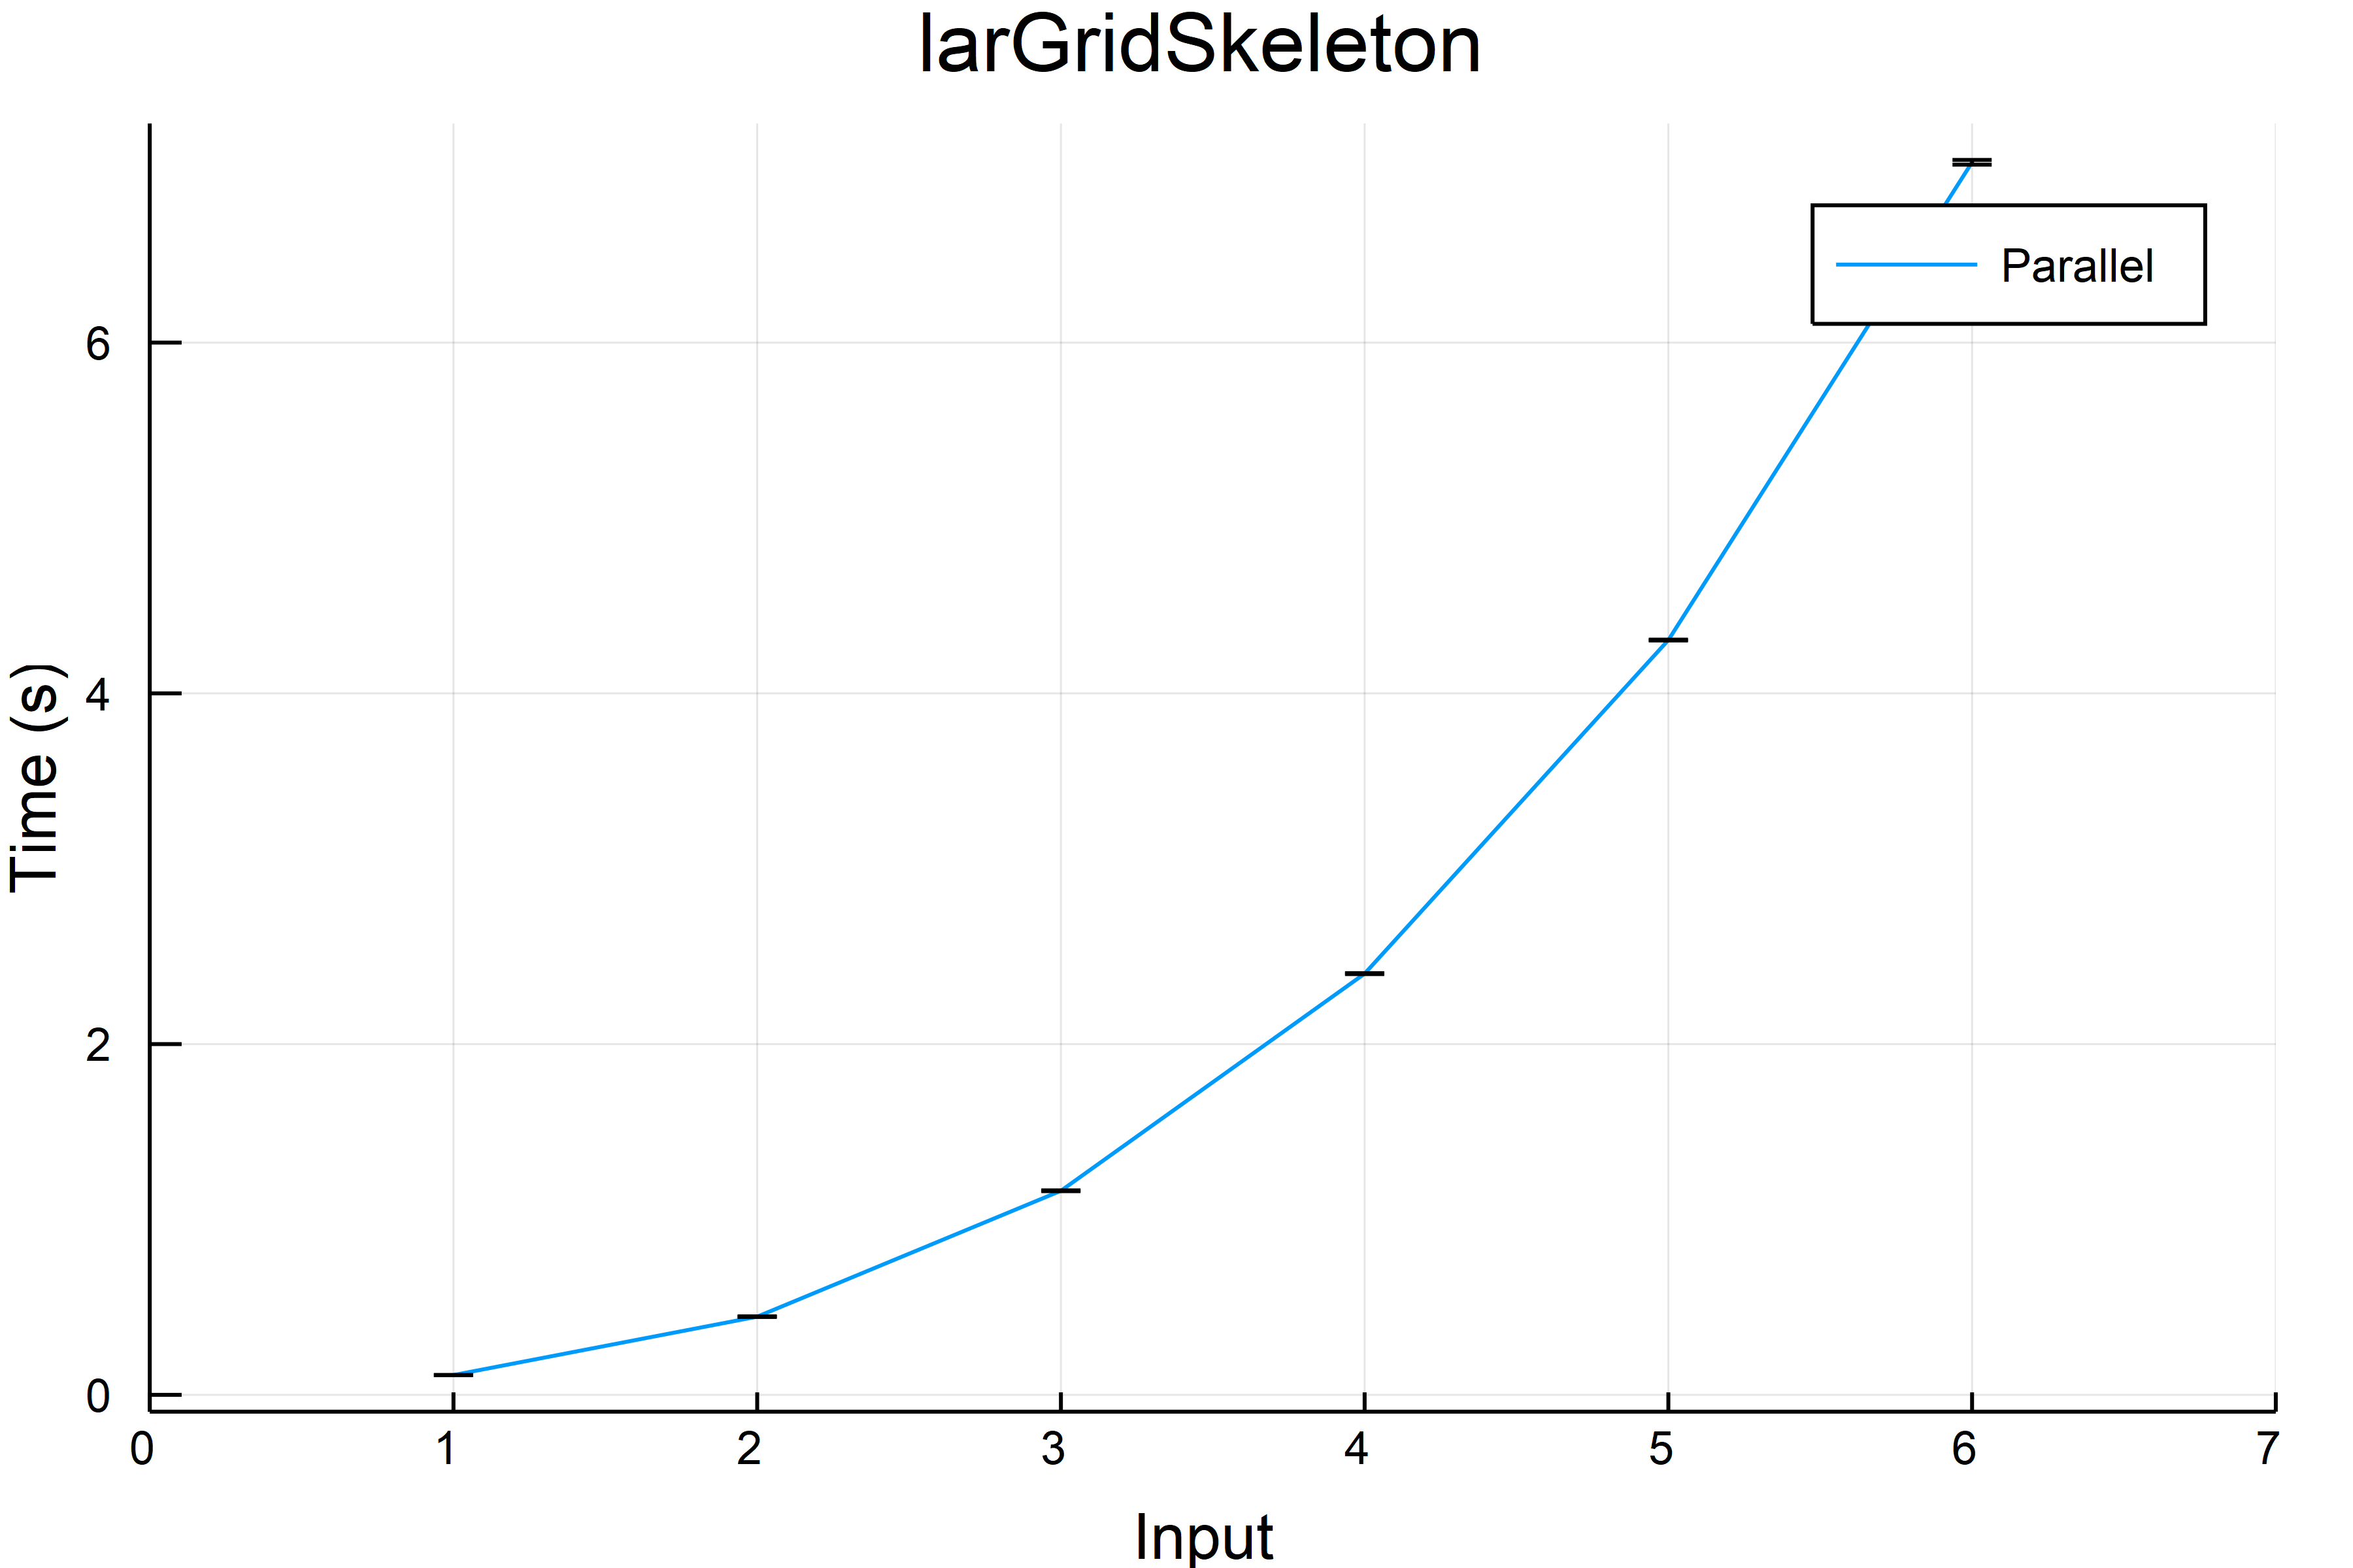
\includegraphics[scale=0.06]{larGridSkeletonPar.png}
\end{figure}

\paragraph{Compare}
\begin{flushleft}\small
\begin{list}{}{} \item
    \begin{Verbatim}[tabsize=4]
x=[xs,xv,xp]
y=[ys,yv,yp]

plot(x,y,yaxis="Time (s)",xlims = (0,length(datap)+1), xaxis="Input", title="larGridSkeleton",
                                                        label=["Serial" "Vectorize" "Parallel"],lw=1)
    \end{Verbatim}
\end{list}
\end{flushleft}   
\begin{figure}[h!]
\centering
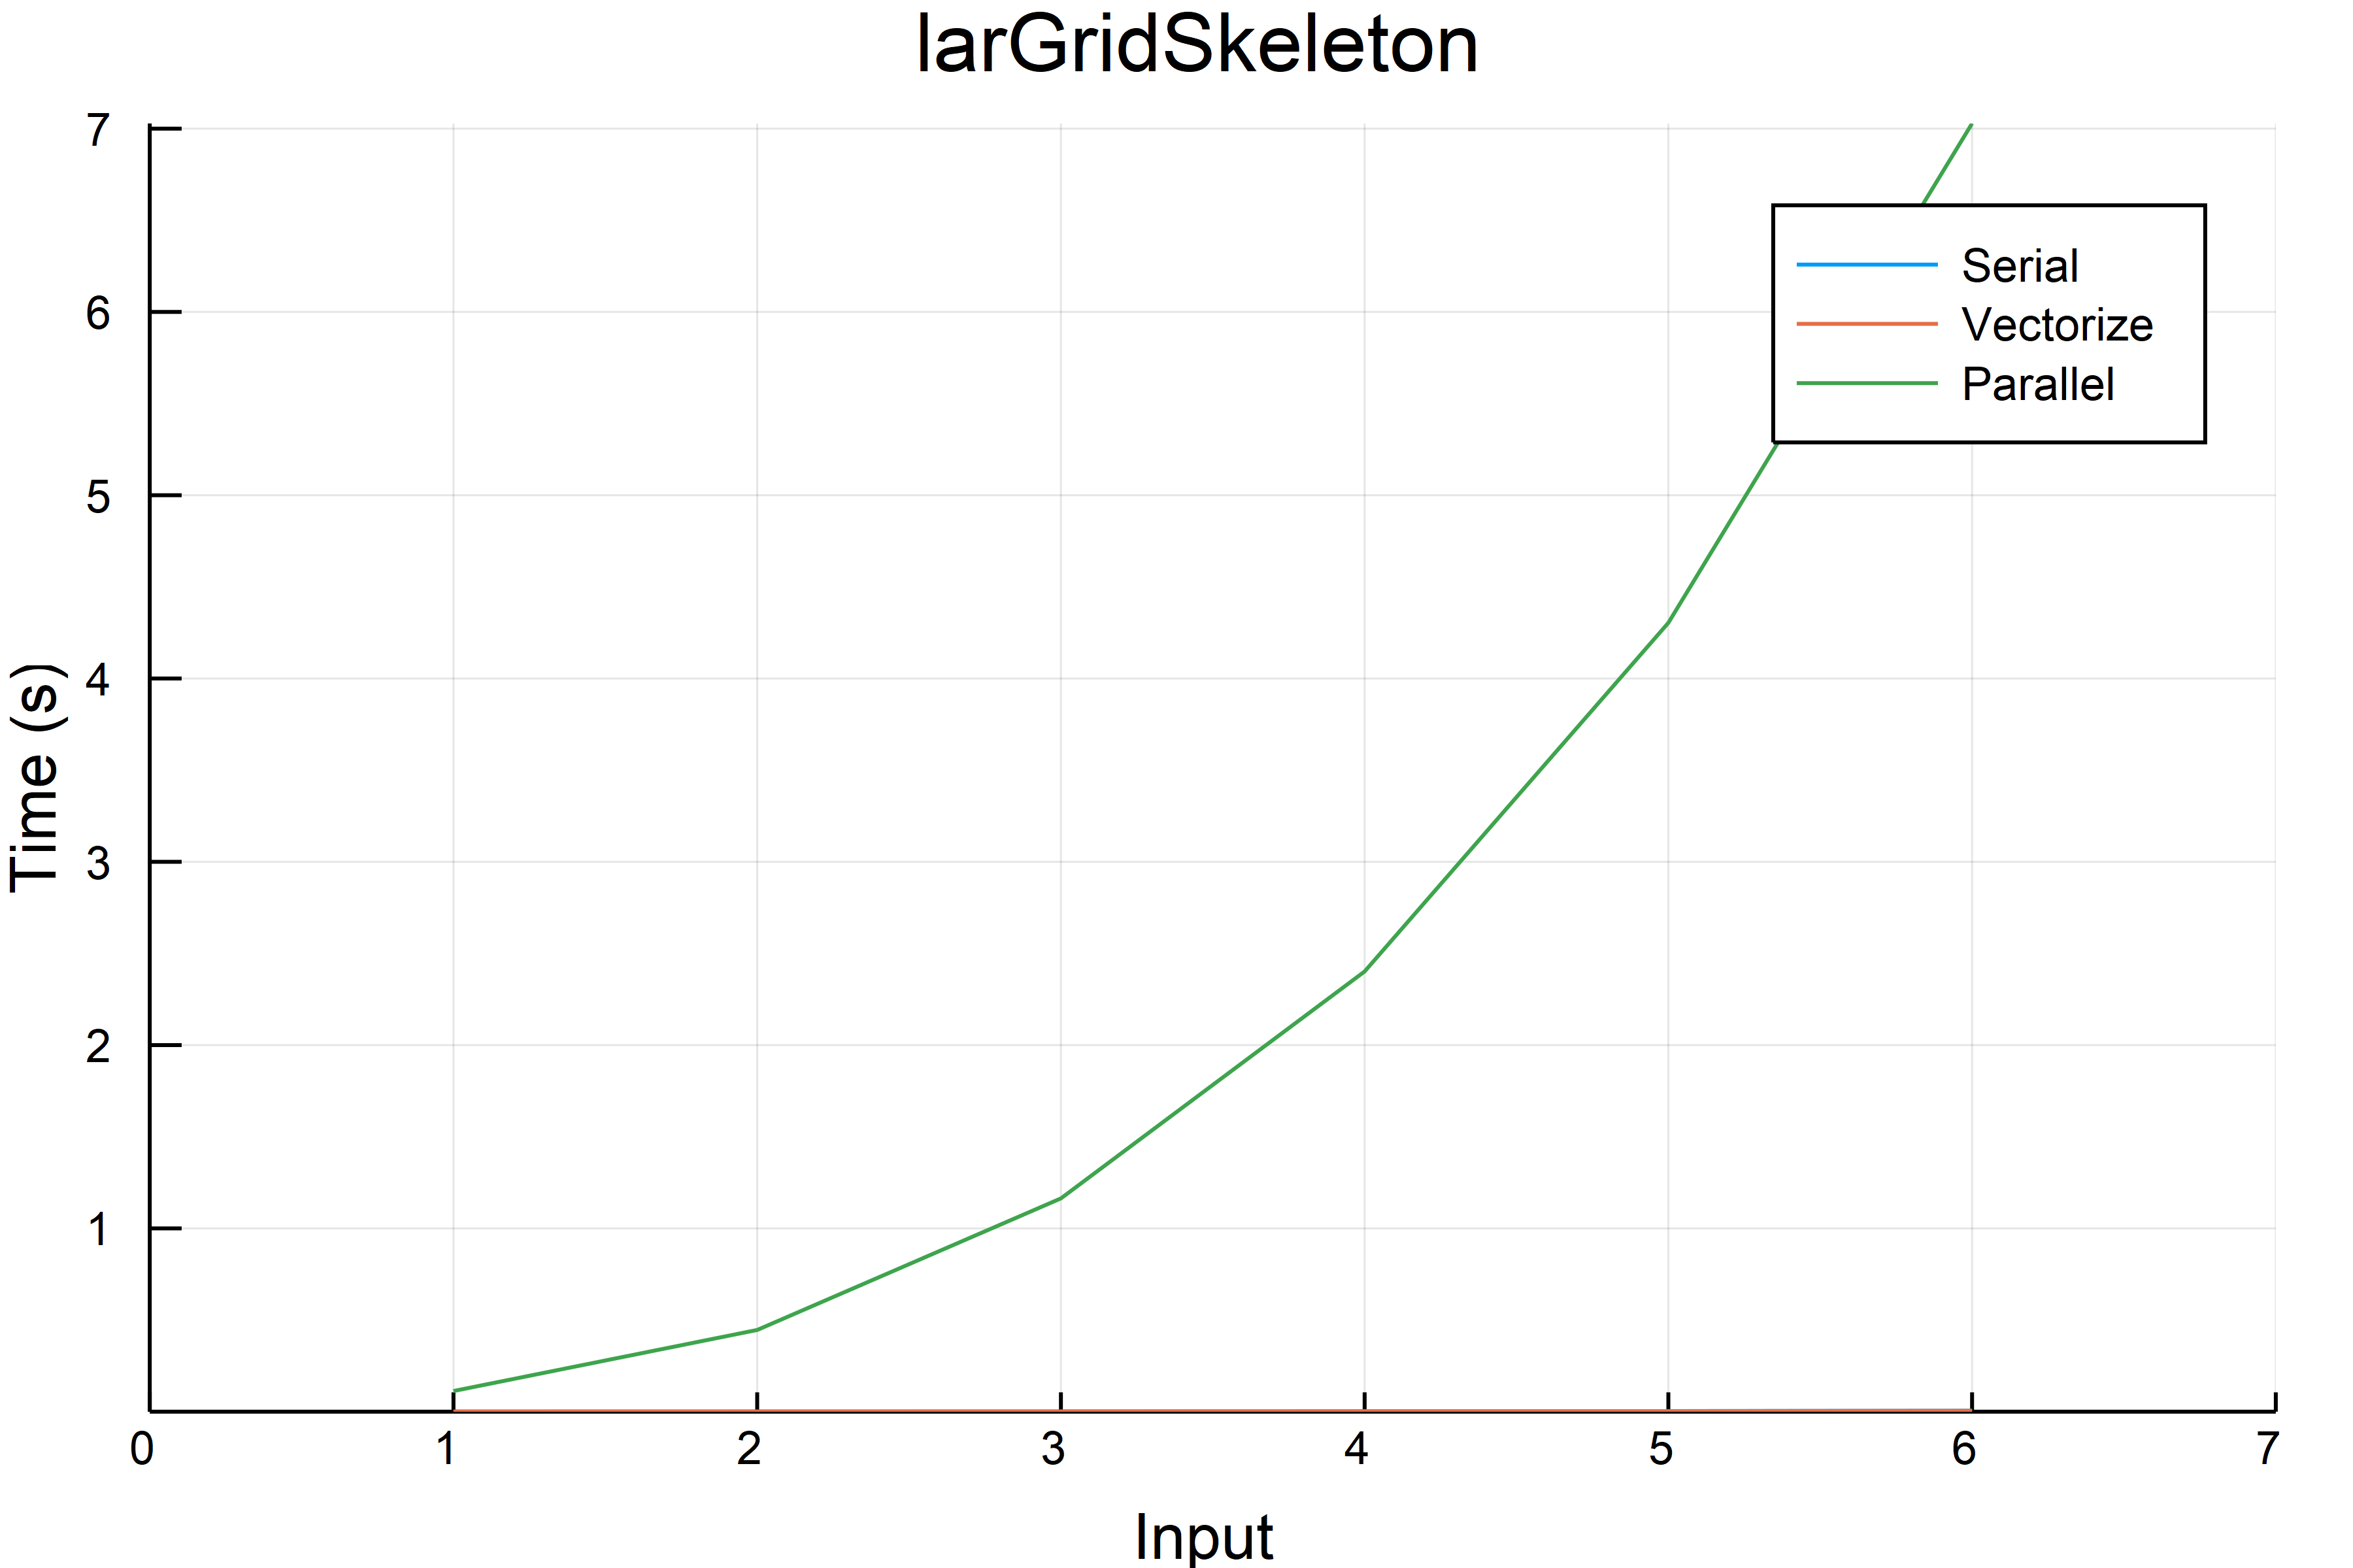
\includegraphics[scale=0.06]{larGridSkeletonCom.png}
\end{figure}

%-------------------------------------------------------------------------------
\subsection{larModelProduct:}

\subsubsection{Translation}
This function has not been parallelized. In particular, first loop of vertices generation, compares previous results, so that it can not be run in parallel mode. Therefore, there is only the translation.
\vspace{1ex}
\begin{flushleft} \small
\begin{center}
\begin{tabular}{|p{16cm}|}
\hline
\cellcolor[gray]{.9}Python\\
\hline
\end{tabular}
\end{center}
\vspace{2ex}
\begin{list}{}{} \item
\begin{Verbatim}[tabsize=4]
def larModelProduct(twoModels):
    (V, cells1), (W, cells2) = twoModels
    vertices = collections.OrderedDict(); k = 0
    for v in V:
        for w in W:
            id = tuple(v+w)
            if not vertices.has_key(id):
                vertices[id] = k
                k += 1   
    cells = [[vertices[tuple(V[v] + W[w])] for v in c1 for w in c2] for c1 in cells1 for c2 in cells2] 
    model = [list(v) for v in vertices.keys()], cells
    return model
\end{Verbatim}
\end{list}
\vspace{2ex}
\begin{center}
\begin{tabular}{|p{16cm}|}
\hline
\cellcolor[gray]{.9}Julia\\
\hline
\end{tabular}
\end{center}
\vspace{2ex}
\begin{list}{}{} \item
\begin{Verbatim}[tabsize=4]
function larModelProduct( modelOne, modelTwo )
    (V, cells1) = modelOne
    (W, cells2) = modelTwo

    vertices = DataStructures.OrderedDict(); 
    k = 1
    for j in 1:size(V,2)
       v = V[:,j]
        for i in 1:size(W,2)
          w = W[:,i]
            id = [v;w]
            if haskey(vertices, id) == false
                vertices[id] = k
                k = k + 1
            end
        end
    end
    
    cells = []
    for c1 in cells1
        for c2 in cells2
            cell = []
            for vc in c1
                for wc in c2 
                    push!(cell, vertices[[V[:,vc];W[:,wc]]])
                end
            end
            push!(cells, cell)
        end
    end
    vertexmodel = []
    for v in keys(vertices)
        push!(vertexmodel, v)
    end
    verts = hcat(vertexmodel...)
    cells = [[v for v in cell] for cell in cells]
    return (verts, cells)
end

function larModelProduct(twoModels)
    modelOne, modelTwo = twoModels
    larModelProduct(modelOne, modelTwo)
end
\end{Verbatim}
\end{list}
\vspace{-1ex}
\footnotesize\addtolength{\baselineskip}{-1ex}
\end{flushleft}
The \texttt{larModelProduct} function takes as input a pair of LAR models and returns the model of their Cartesian product. LAR model is a pair (geometry, topology), so this function create the right set of vertices and cells of the output model, using $dictionaries$. \texttt{OrderedDict()}, which comes from the package \texttt{DataStructures}, creates ordered dictionaries, that are simply dictionaries whose entries have a particular order. The order refers to insertion order, which allows deterministic iteration over the dictionary or set.
\newpage
\subsubsection{Test}
\begin{center}
\begin{tabular}{|p{16cm}|}
\hline
\cellcolor[gray]{.9}Test\\
\hline
\end{tabular}
\end{center}

\begin{flushleft}\small
\begin{list}{}{} \item
\begin{Verbatim}[tabsize=4]
@testset "larModelProduct" begin
	geom_0,topol_0 = larSplit(2)(3),[[1,2],[2,3],[3,4]]
	geom_1,topol_1 = larSplit(3)(2), [[1,2],[2,3]]
	mod_0 = (geom_0,topol_0)
	mod_1 = (geom_1,topol_1)
	V,CV = larModelProduct([mod_0,mod_1])
	@test size(V,2)==12
	@test length(CV)==6
end

\end{Verbatim}
\end{list}
\end{flushleft}
%-------------------------------------------------------------------------------

\subsection{larCuboids:}

\subsubsection{Translation}
Here, translation is simple. This function generates cuboidal complex in full-dimensions and it's also possible include cells of all dimensions, depending on the Boolean value of the \texttt{full} parameter.
\vspace{1ex}
\begin{flushleft} \small
\begin{center}
\begin{tabular}{|p{16cm}|}
\hline
\cellcolor[gray]{.9}Python\\
\hline
\end{tabular}
\end{center}
\vspace{2ex}
\begin{list}{}{} \item
\begin{Verbatim}[tabsize=4]
def larImageVerts(shape):
   def vertexDomain(n): 
      return [[k] for k in range(n)]
   vertLists = [vertexDomain(k+1) for k in shape]
   vertGrid = larVertProd(vertLists)
   return vertGrid

def larCuboids(shape, full=False):
   vertGrid = larImageVerts(shape)
   gridMap = larGridSkeleton(shape)
   if not full: 
      cells = gridMap(len(shape))
   else:
      skeletonIds = range(len(shape)+1)
      cells = [ gridMap(id) for id in skeletonIds ]
   return vertGrid, cells
\end{Verbatim}
\end{list}
\begin{center}
\vspace{2ex}
\begin{tabular}{|p{16cm}|}
\hline
\cellcolor[gray]{.9}Julia\\
\hline
\end{tabular}
\end{center}
\vspace{2ex}
\begin{list}{}{} \item
\begin{Verbatim}[tabsize=4]
function vertexDomain(n)
   return hcat([k for k in 0:n-1]...)
end

function larImageVerts(shape)
   vertLists = [vertexDomain(k+1) for k in shape]
   vertGrid = larVertProd(vertLists)
   return vertGrid
end

function larCuboids(shape, full=false)
   vertGrid = larImageVerts(shape)
   gridMap = larGridSkeleton(shape)
   if ! full
      cells = gridMap(length(shape))
   else
      skeletonIds = 0:length(shape)
      cells = [ gridMap(id) for id in skeletonIds ]
   end
   return vertGrid, cells
end
\end{Verbatim}
\end{list}

\end{flushleft}

\vspace{2ex}

\subsubsection{Vectorize}
In this function it's possible vectorize $gridMap$, that is the first application of function \texttt{larGridSkeleton}, on lenght of $shape$ takes in input.
\vspace{1ex}
\begin{flushleft} \small
\begin{center}
\begin{tabular}{|p{16cm}|}
\hline
\cellcolor[gray]{.9}Vectorized code\\
\hline
\end{tabular}
\end{center}
\vspace{2ex}
\begin{list}{}{} \item
   \begin{Verbatim}[tabsize=4]
function vlarCuboids(shape, full=false)
    vertGrid = vlarImageVerts(shape)
    gridMap = vlarGridSkeleton(shape)
    if ! full
        cells = gridMap(length(shape))
    else
        skeletonIds = 0:length(shape)
        cells = gridMap.(skeletonIds)
    end
    return vertGrid, cells
end
   \end{Verbatim}
\end{list}
\end{flushleft}
\vspace{2ex}

\subsubsection{Parallel computing}
\vspace{1ex}
\begin{flushleft} \small
\begin{center}
\begin{tabular}{|p{16cm}|}
\hline
\cellcolor[gray]{.9}Parallel\\
\hline
\end{tabular}
\end{center}
\vspace{2ex}
\begin{list}{}{} \item
   \begin{Verbatim}[tabsize=4]
@everywhere function vertexDomain(n)
   return hcat([k for k in 0:n-1]...)
end

@everywhere function plarImageVerts(shape)
   vertLists = @parallel (vcat) for k in shape 
                [vertexDomain(k+1)]
                end
   vertGrid = larVertProd(vertLists)
   return vertGrid
end

@everywhere function plarCuboids(shape, full=false)
    vertGrid = plarImageVerts(shape)
    gridMap = plarGridSkeleton(shape)
    if ! full
        cells = gridMap(length(shape))
    else
        skeletonIds = 0:length(shape)
        cells = [ gridMap(id) for id in skeletonIds ]
    end
    return vertGrid, cells
end
   \end{Verbatim}
\end{list}
\end{flushleft}
\subsubsection{Test}
\begin{center}
\begin{tabular}{|p{16cm}|}
\hline
\cellcolor[gray]{.9}Test\\
\hline
\end{tabular}
\end{center}

\begin{flushleft}\small
\begin{list}{}{} \item
\begin{Verbatim}[tabsize=4]
@testset "LarImageVerts Tests" "$shape" for shape in [[3,2,1],[3,2],[10,10,10]]
		@test size(larImageVerts(shape)) == (length(shape),prod(shape + 1))
end

@testset "vLarImageVerts Tests" "$shape" for shape in [[3,2,1],[3,2],[10,10,10]]
		    @test size(vlarImageVerts(shape)) == (length(shape),prod(shape + 1))
end

@testset "larCuboids" begin
	V,CV=larCuboids([1,1,1])
	@test size(V,2)==8
	@test length(CV)==1
end

\end{Verbatim}
\end{list}
\end{flushleft}
\subsubsection{Execution time}
\begin{center}
\begin{tabular}{|p{16cm}|}
\hline
\cellcolor[gray]{.9}Execution time\\
\hline
\end{tabular}
\end{center}


\paragraph{Serial}
\begin{flushleft}\small
\begin{list}{}{} \item
    \begin{Verbatim}[tabsize=4]
datas=[Time(N,larCuboids,[j,j,j]) for j in range(1,30)]

xs=[1:length(datas);]
ys=mean.(datas)
yerrs=std.(datas)/sqrt(N)

plot(xs,ys,yaxis="Time (s)",xlims = (0,length(datas)+1), yerr = yerrs, xaxis="Input", 
                                                title="larCuboids",label=["Serial"],lw=1)
    \end{Verbatim}
\end{list}
\end{flushleft} 

\paragraph{Vectorize}
\begin{flushleft}\small
\begin{list}{}{} \item
    \begin{Verbatim}[tabsize=4]
datav=[Time(N,vlarCuboids,[j,j,j]) for j in range(1,30)]

xv=[1:length(datav);]
yv=mean.(datav)
yerrv=std.(datav)/sqrt(N)

plot(xv,yv,yaxis="Time (s)",xlims = (0,length(datav)+1), yerr = yerrv, xaxis="Input", 
                                                title="larCuboids",label=["Vectorize"],lw=1)
    \end{Verbatim}
\end{list}
\end{flushleft}

\begin{figure}[h!]
\centering
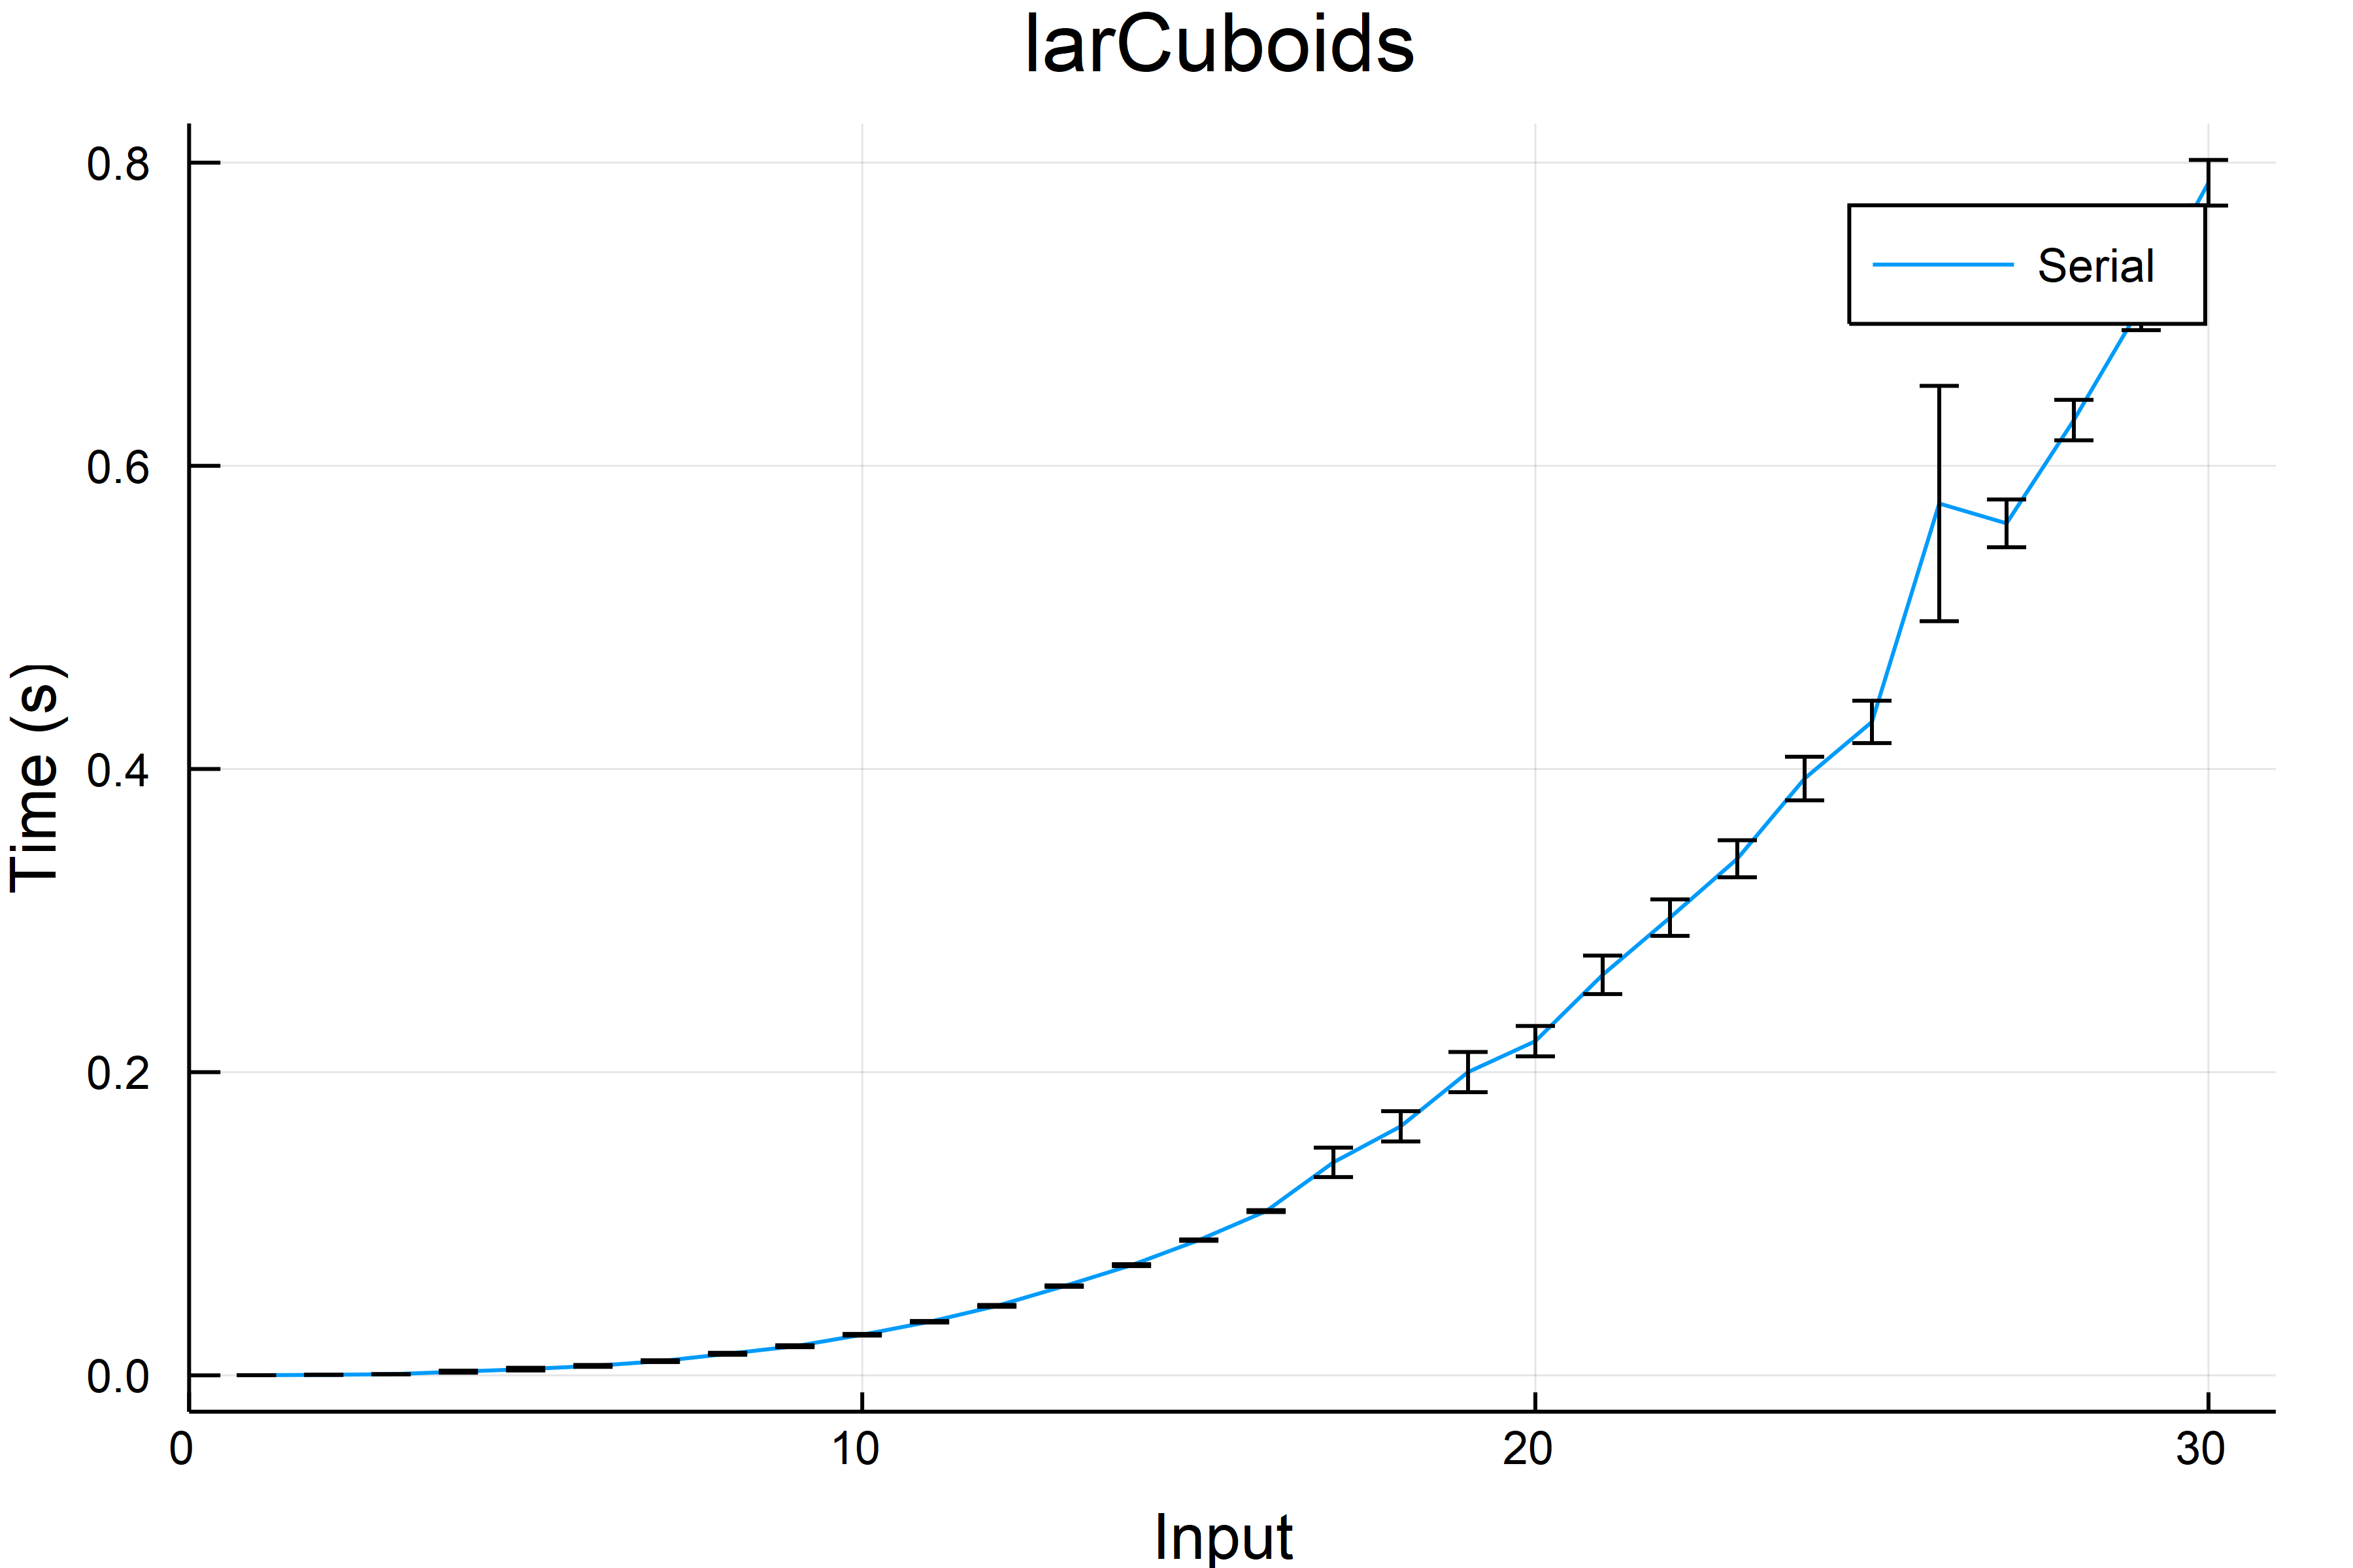
\includegraphics[scale=0.06]{larCuboidsSer.png}
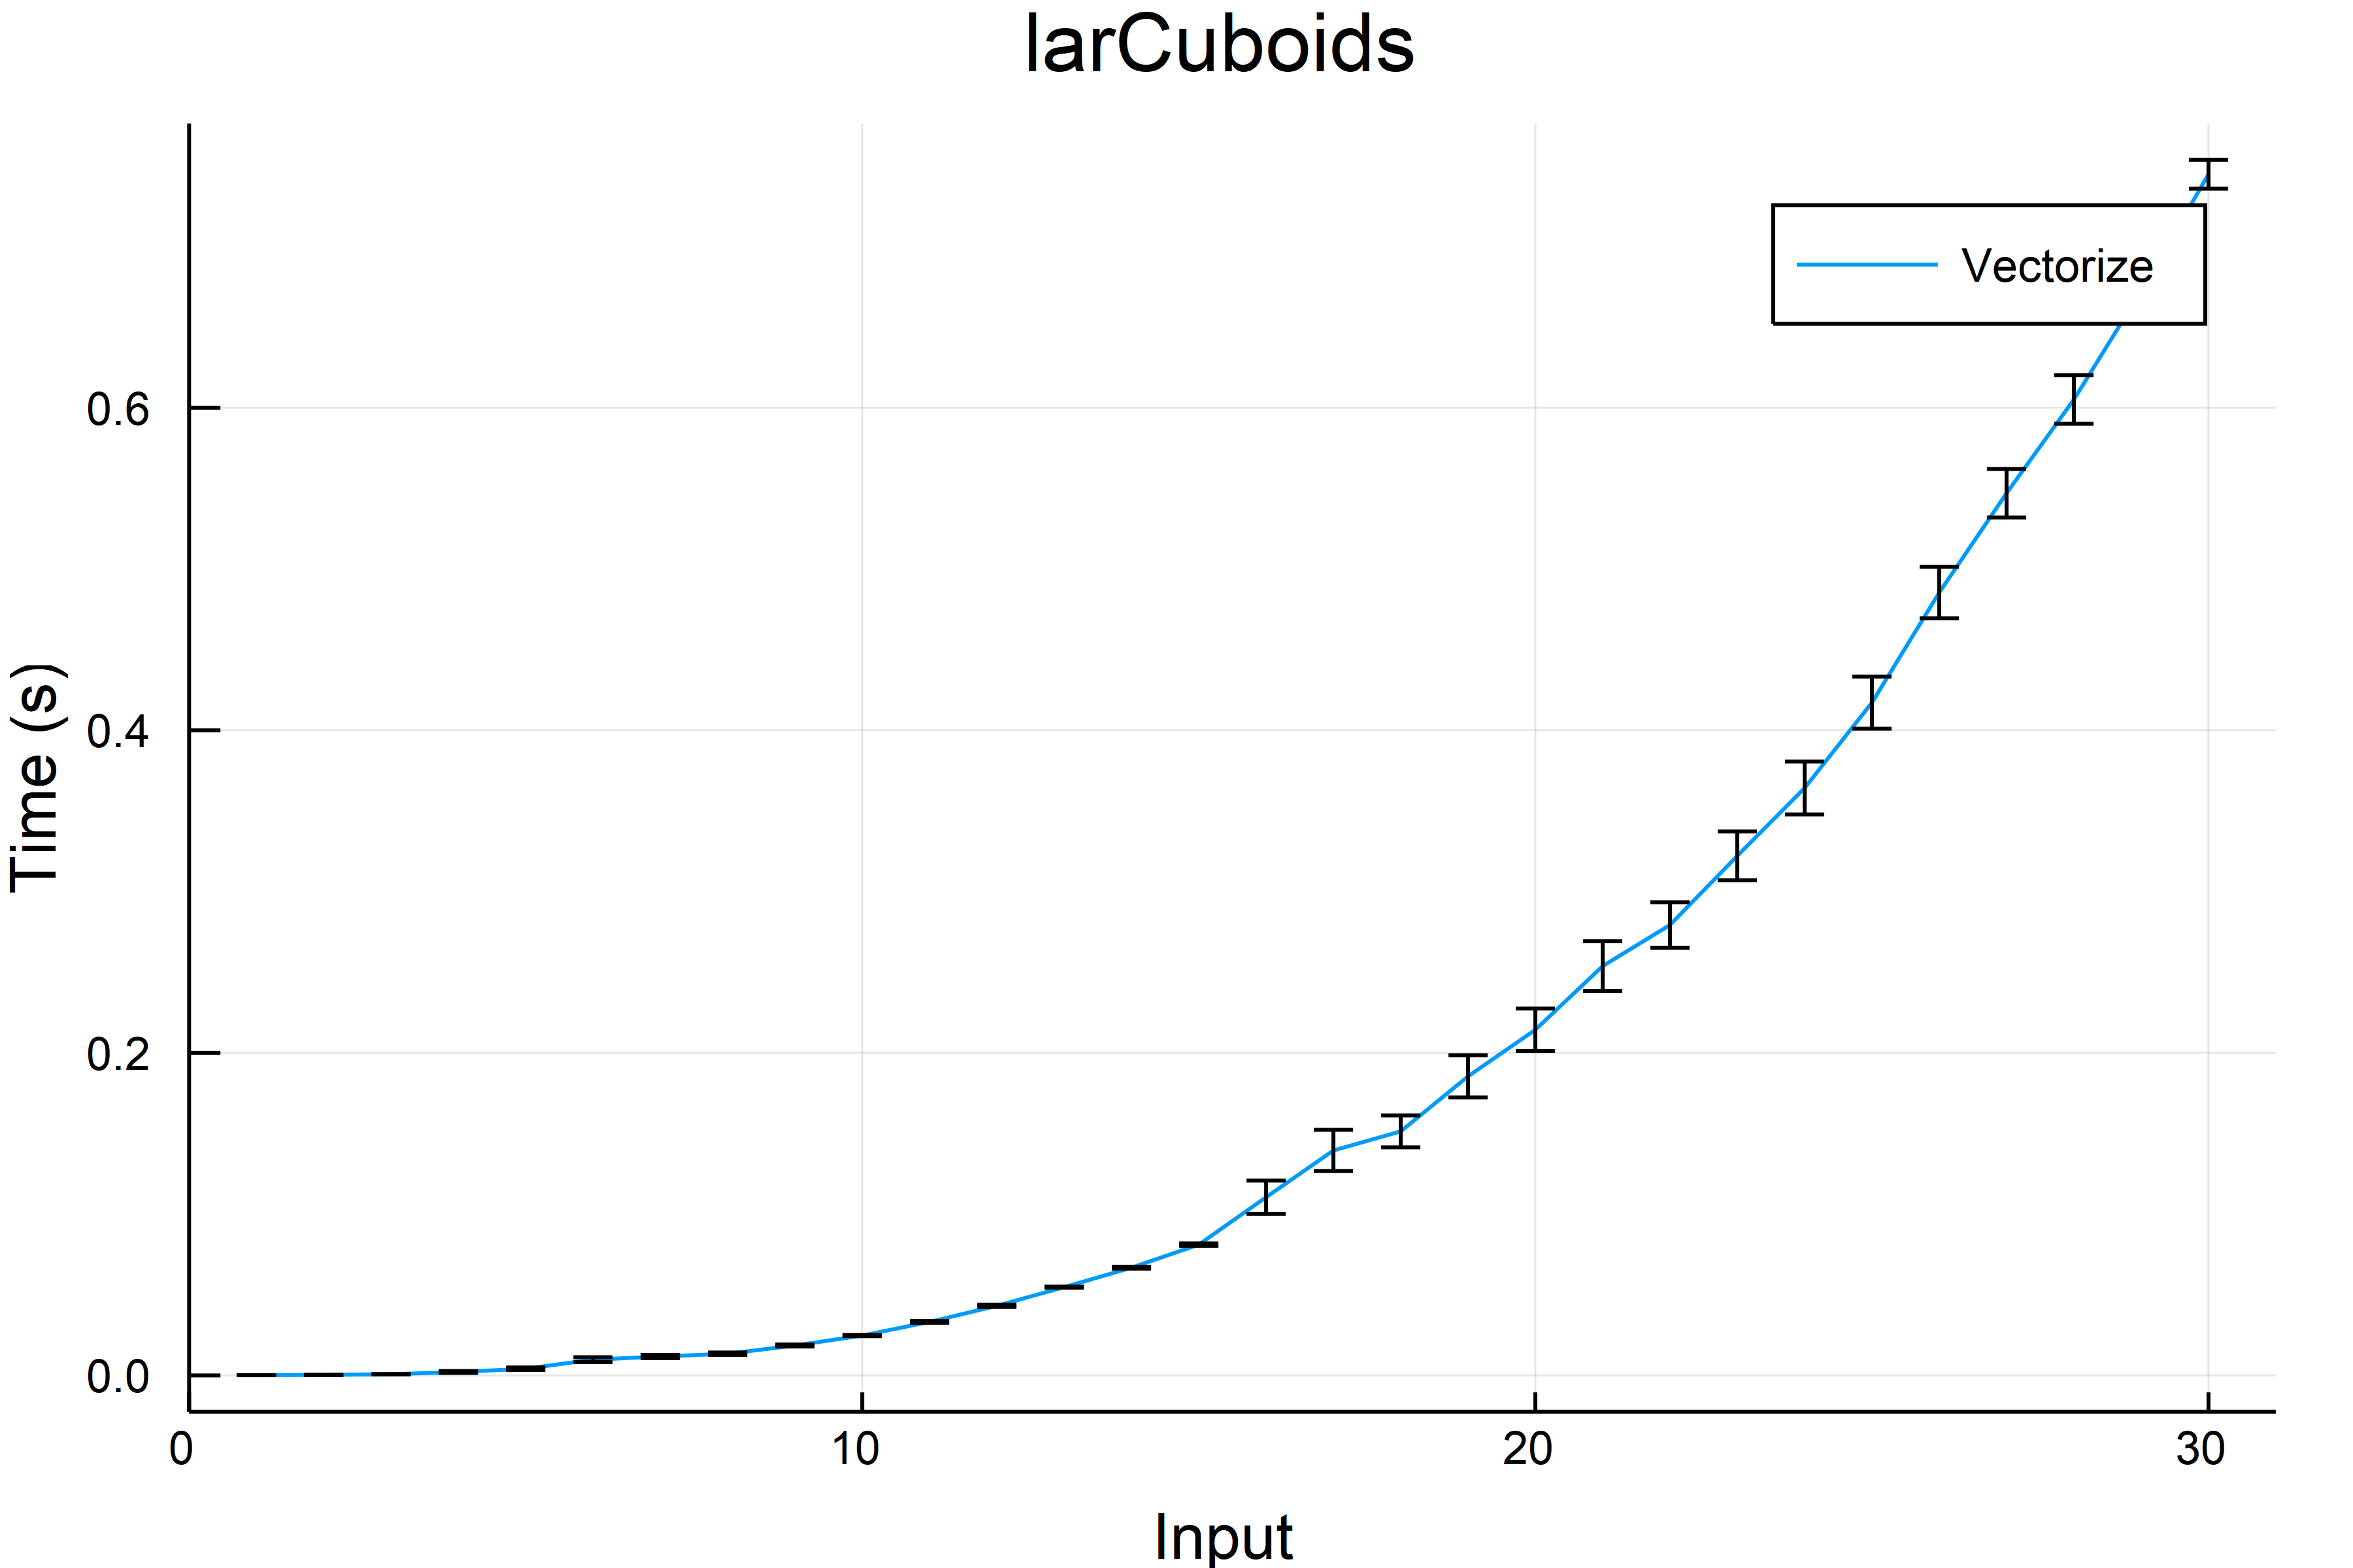
\includegraphics[scale=0.06]{larCuboidsVec.png}
\end{figure}

\paragraph{Compare}
\begin{flushleft}\small
\begin{list}{}{} \item
    \begin{Verbatim}[tabsize=4]
x=[xs,xv]
y=[ys,yv]

plot(x,y,yaxis="Time (s)",xlims = (0,length(datav)+1), xaxis="Input", title="larCuboids",
                                                label=["Serial" "Vectorize" "Parallel"],lw=1)

    \end{Verbatim}
\end{list}
\end{flushleft}   

\begin{figure}[h!]
\centering
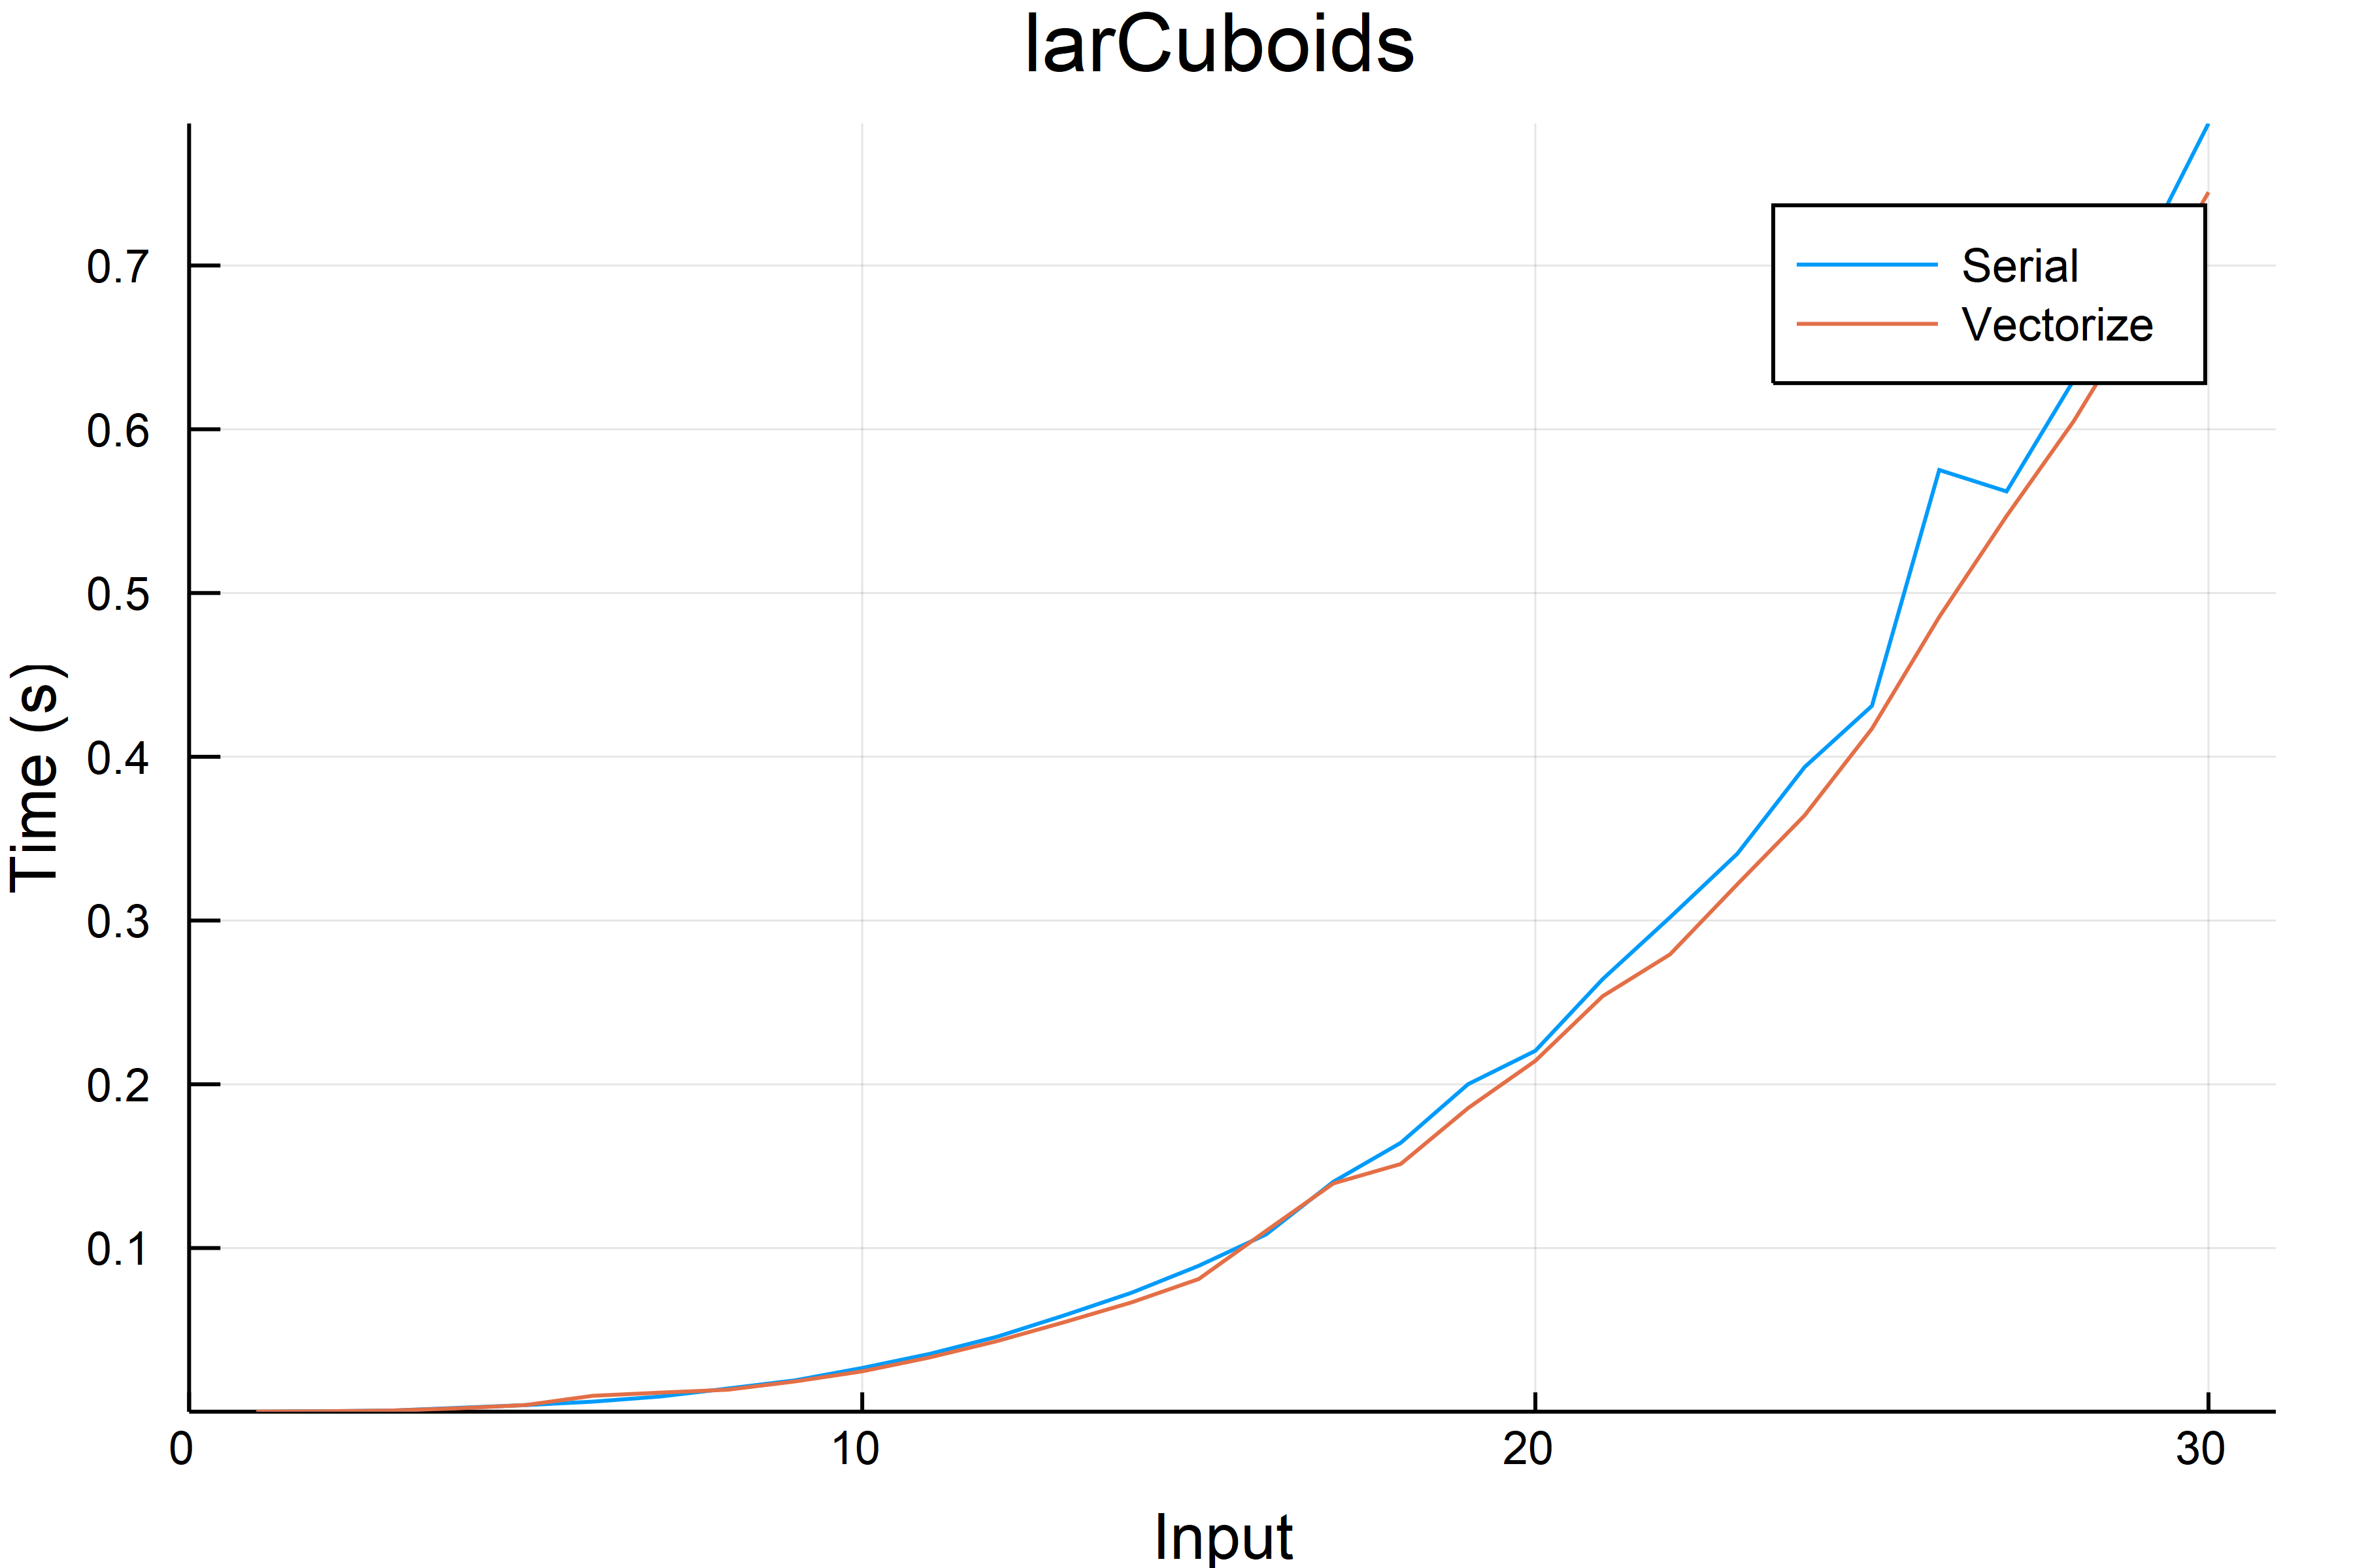
\includegraphics[scale=0.06]{larCuboidsCom1.png}
\end{figure}

\paragraph{Parallel}
\begin{flushleft}\small
\begin{list}{}{} \item
    \begin{Verbatim}[tabsize=4]
datap=[Time(N,plarCuboids,[j,j,j]) for j in range(1,6)]

xp=[1:length(datap);]
yp=mean.(datap)
yerrp=std.(datap)/sqrt(N)

plot(xp,yp,yaxis="Time (s)",xlims = (0,length(datav)+1), yerr = yerrp, xaxis="Input", 
                                                title="larCuboids",label=["Parallel"],lw=1)
 \end{Verbatim}
\end{list}
\end{flushleft}   

\begin{figure}[h!]
\centering
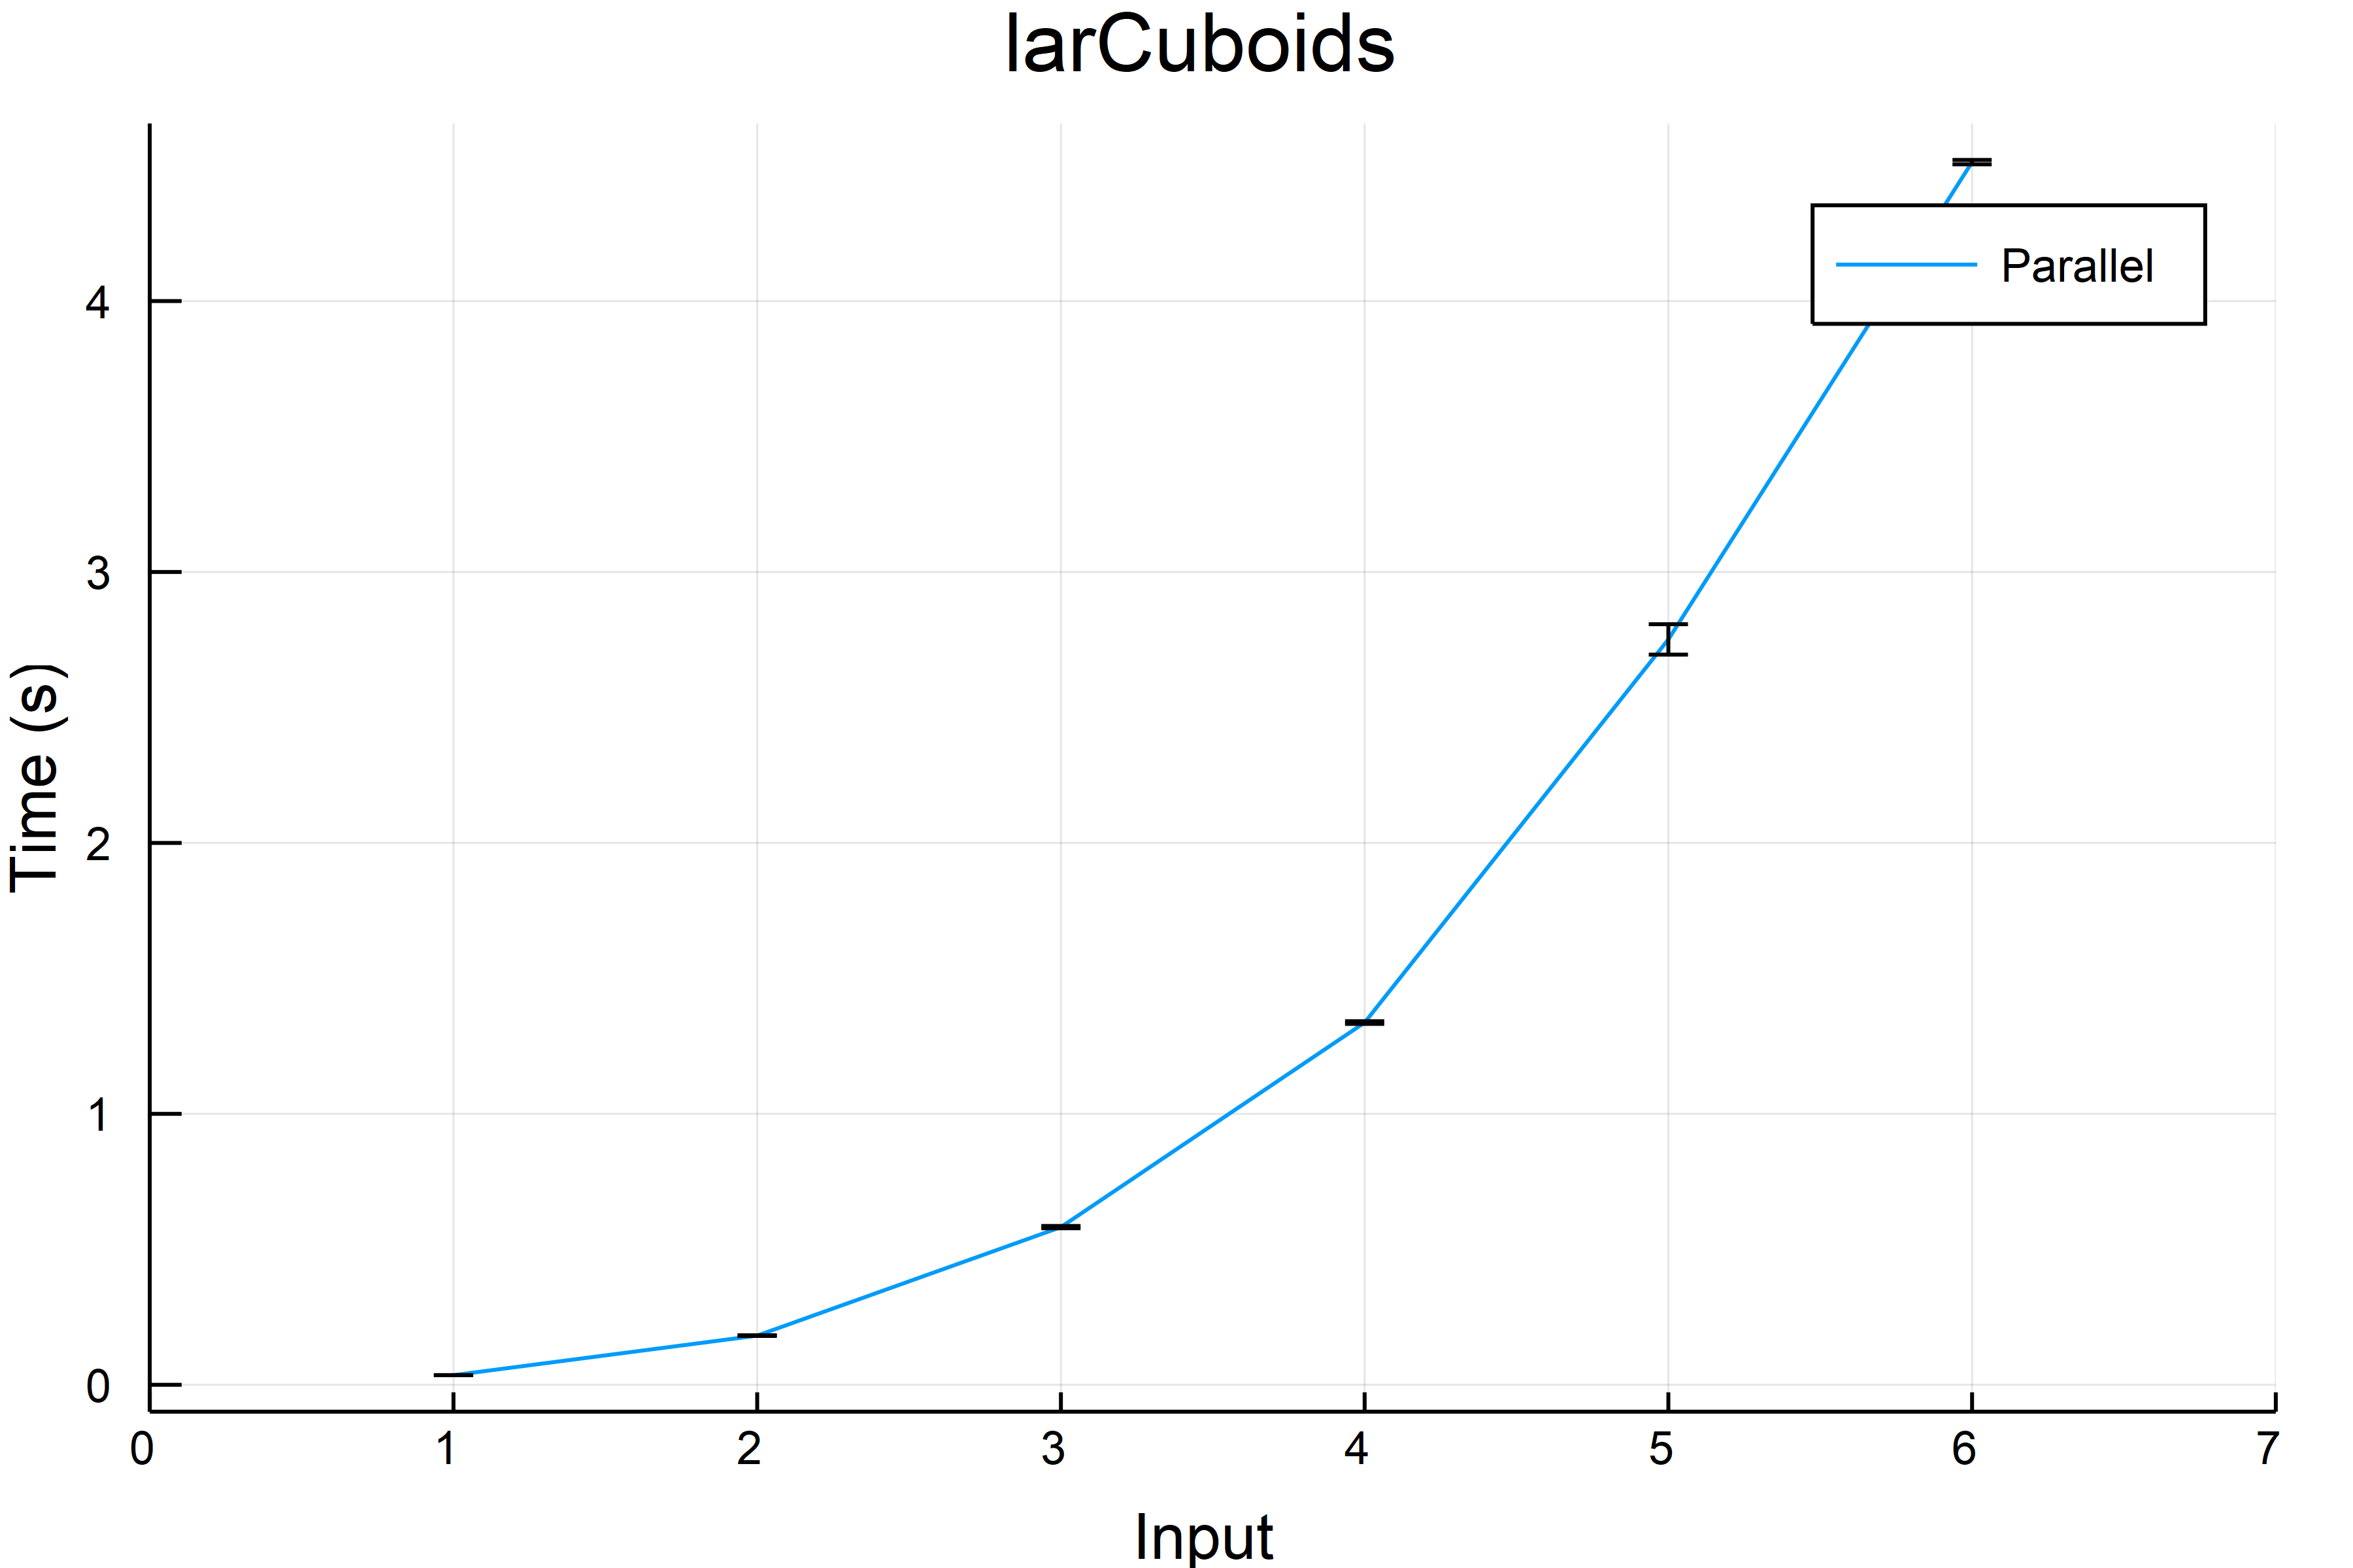
\includegraphics[scale=0.06]{larCuboidsPar.png}
\end{figure}

\paragraph{Compare}
\begin{flushleft}\small
\begin{list}{}{} \item
    \begin{Verbatim}[tabsize=4]
x=[xs,xv,xp]
y=[ys,yv,yp]

plot(x,y,yaxis="Time (s)",xlims = (0,length(datav)+1), xaxis="Input", title="larCuboids",
                                                    label=["Serial" "Vectorize" "Parallel"],lw=1)
    \end{Verbatim}
\end{list}
\end{flushleft}  

\begin{figure}[h!]
\centering
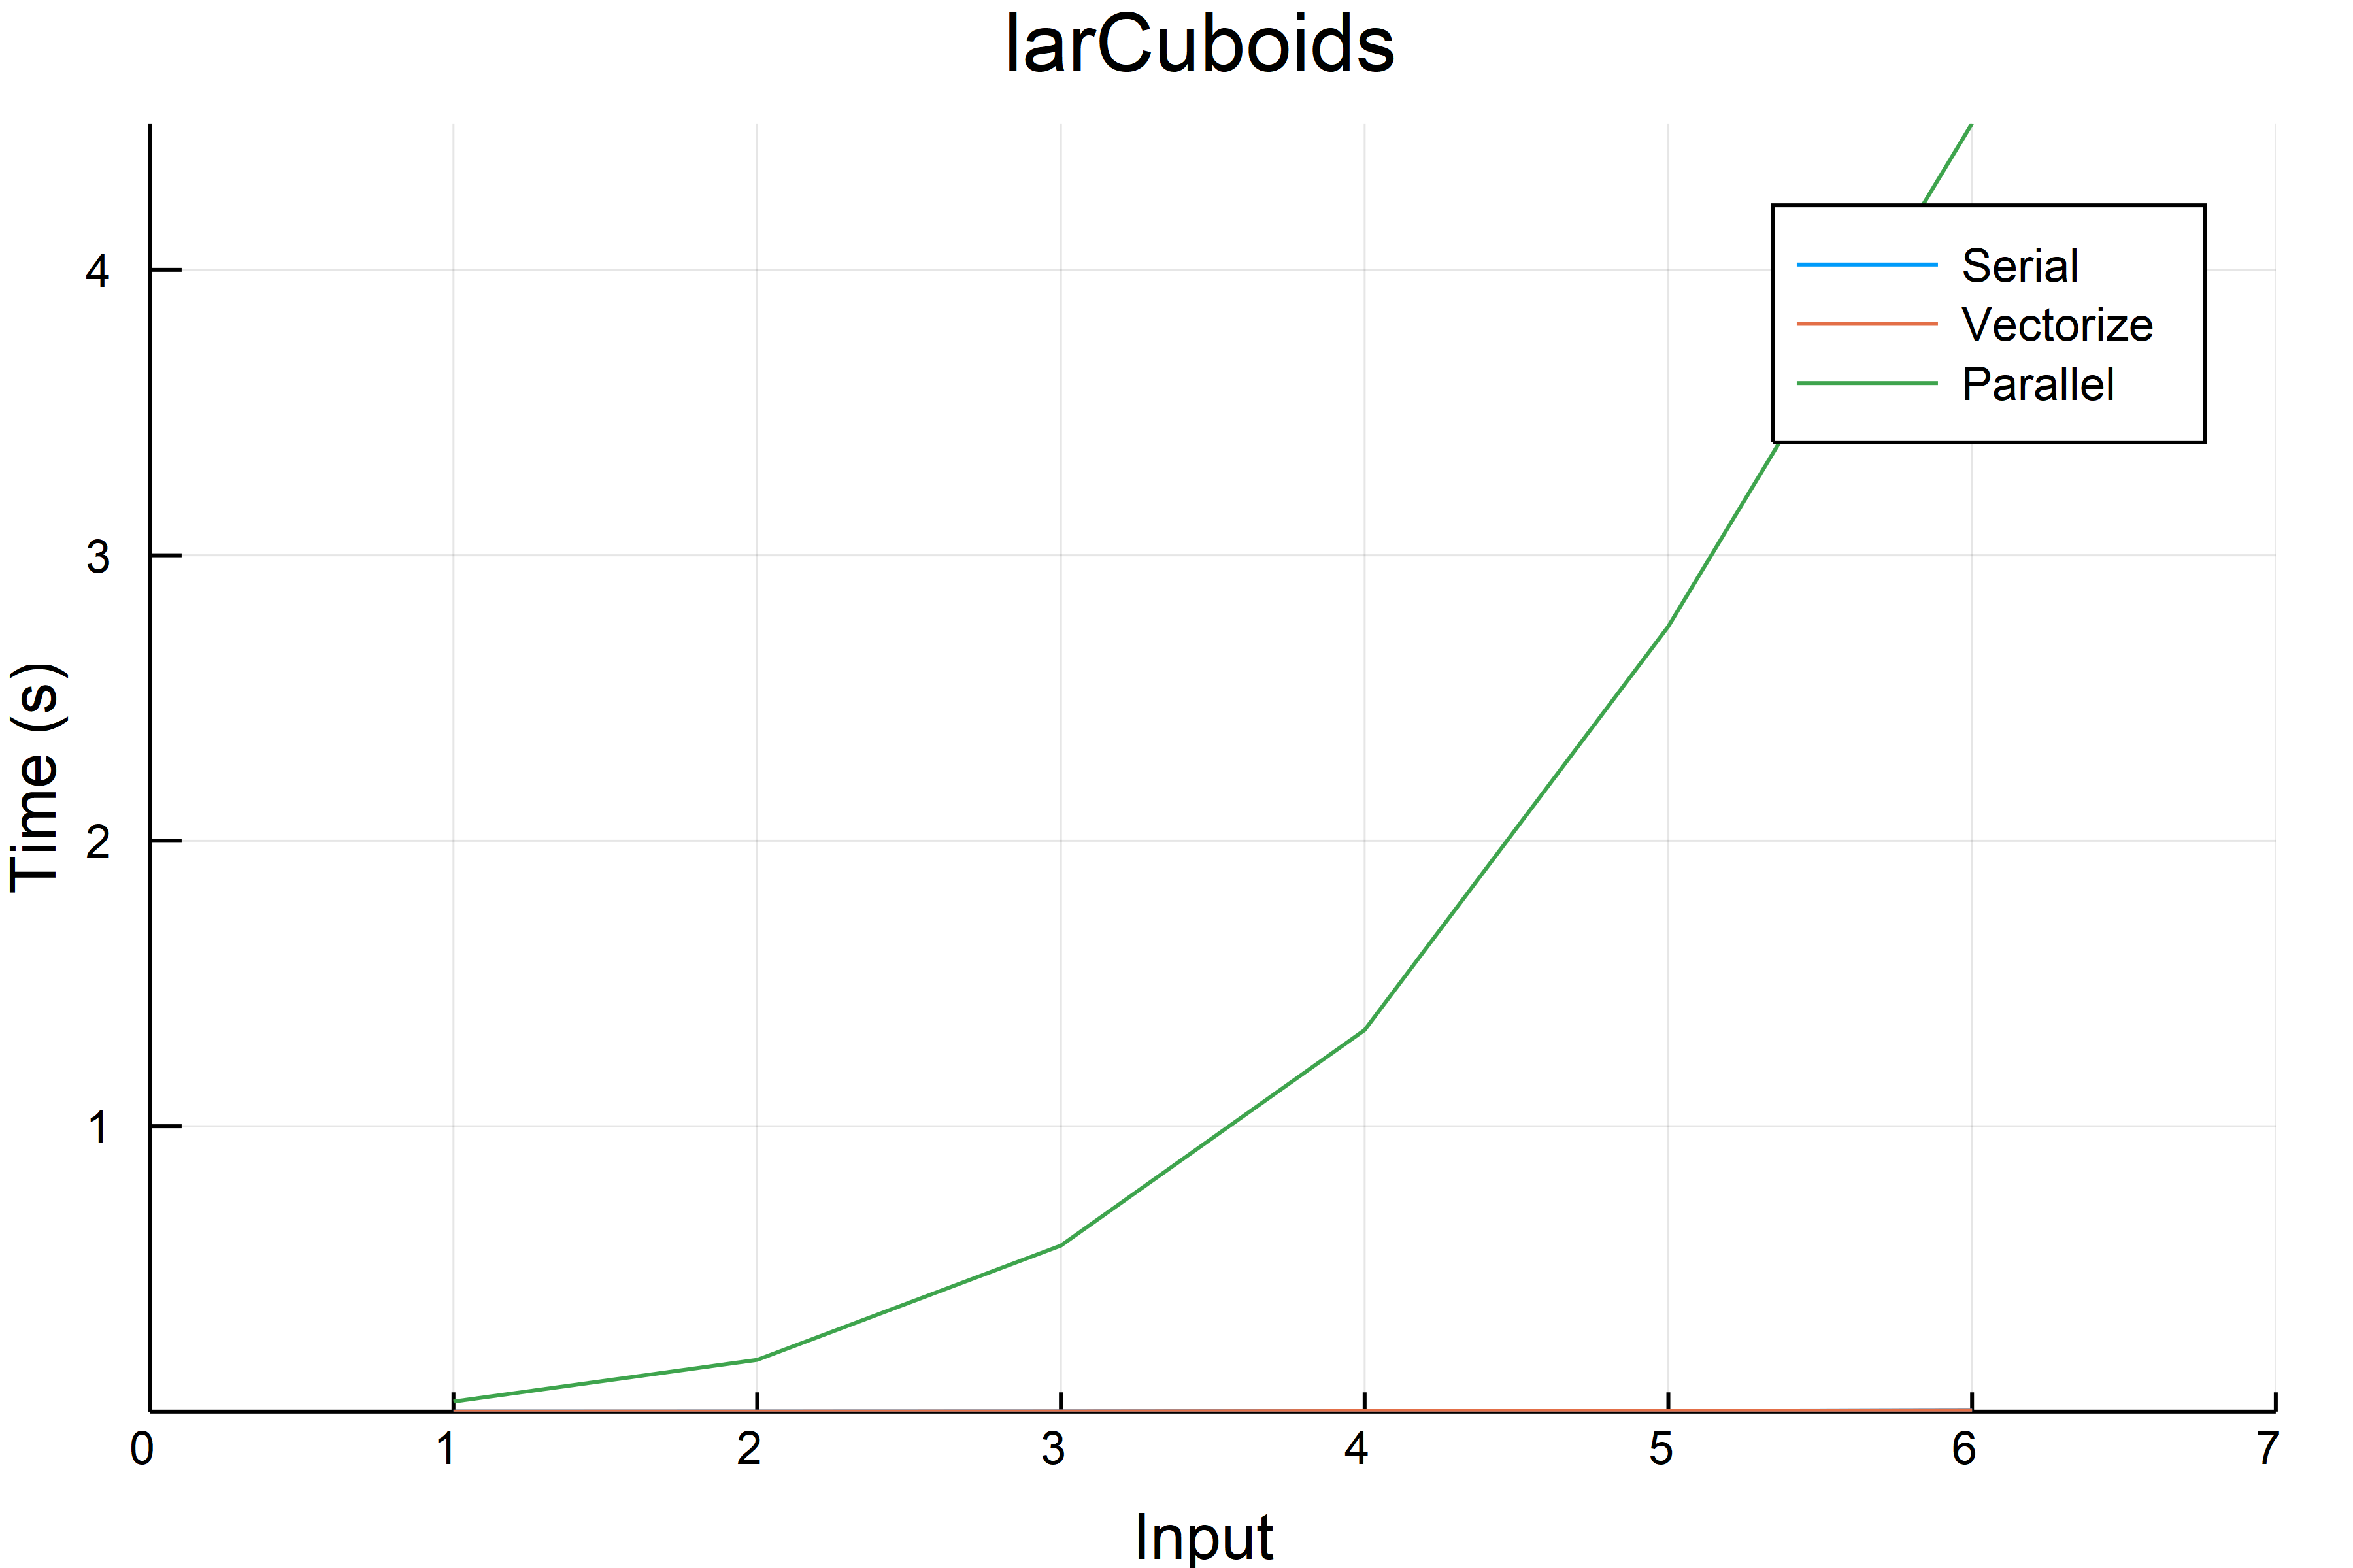
\includegraphics[scale=0.06]{larCuboidsCom.png}
\end{figure}


%-------------------------------------------------------------------------------
\subsection{gridSkeletons:}
\subsubsection{Translation}
\begin{flushleft} \small

\vspace{1ex}
\begin{center}
\begin{tabular}{|p{16cm}|}
\hline
\cellcolor[gray]{.9}Python\\
\hline
\end{tabular}
\end{center}


\begin{list}{}{} \item
\begin{Verbatim}[tabsize=4]
def gridSkeletons(shape):
   gridMap = larGridSkeleton(shape)
   skeletonIds = range(len(shape)+1)
   skeletons = [gridMap(id) for id in skeletonIds]
   return skeletons
\end{Verbatim}
\end{list}

\begin{center}
\begin{tabular}{|p{16cm}|}
\hline
\cellcolor[gray]{.9}Julia\\
\hline
\end{tabular}
\end{center}

\begin{list}{}{} \item
\begin{Verbatim}[tabsize=4]
function gridSkeletons(shape)
    gridMap = larGridSkeleton(shape)
    skeletonIds = range(0,length(shape)+1)
    skeletons = [gridMap(id) for id in skeletonIds]
    return skeletons
end
\end{Verbatim}
\end{list}

\vspace{2ex}

\subsubsection{Vectorize}
\vspace{1ex}
\begin{center}
\begin{tabular}{|p{16cm}|}
\hline
\cellcolor[gray]{.9}Vectorized code\\
\hline
\end{tabular}
\end{center}
\begin{list}{}{} \item
   \begin{Verbatim}[tabsize=4]
function vgridSkeletons(shape)
    gridMap = vlarGridSkeleton(shape)
    skeletonIds = range(0,length(shape)+1)
    skeletons = gridMap.(skeletonIds)
    return skeletons
end
   \end{Verbatim}
\end{list}

\vspace{2ex}

\subsubsection{Parallel computing}
\vspace{1ex}
\begin{center}
\begin{tabular}{|p{16cm}|}
\hline
\cellcolor[gray]{.9}Parallel\\
\hline
\end{tabular}
\end{center}
\begin{list}{}{} \item
   \begin{Verbatim}[tabsize=4]
function pgridSkeletons(shape)
    gridMap = plarGridSkeleton(shape)
    skeletonIds = range(0,length(shape)+1)
    skeletons = [gridMap(id) for id in skeletonIds]
    return skeletons
end
   \end{Verbatim}
\end{list}

\vspace{-1ex}
\footnotesize\addtolength{\baselineskip}{-1ex}
\end{flushleft}

\subsubsection{Test}
\begin{center}
\begin{tabular}{|p{16cm}|}
\hline
\cellcolor[gray]{.9}Test\\
\hline
\end{tabular}
\end{center}

\begin{flushleft}\small
\begin{list}{}{} \item
\begin{Verbatim}[tabsize=4]
@testset "gridSkeletons Tests" begin
        @test length(gridSkeletons([3])[1]) == 4
      	@testset "$shape" for shape in [[1,1,1],[3],[2,3]]
			@test length(gridSkeletons(shape)) == length(shape)+1
			@test typeof(gridSkeletons(shape)) == Array{Array{Array{Int64,1},1},1}
		end
		@testset "compare" begin
			@testset "$shape" for shape in [[1,1,1],[2,3],[4]]
			@testset "$d" for d in 0:length(shape)
				@test larGridSkeleton(shape)(d)== gridSkeletons(shape)[d+1] 
				@test typeof(larGridSkeleton(shape)(d)) == Array{Array{Int64,1},1}
			end
			end
		end
end

@testset "vgridSkeletons Tests" begin
            @test length(vgridSkeletons([3])[1]) == 4
      	    @testset "$shape" for shape in [[1,1,1],[3],[2,3]]
			    @test length(vgridSkeletons(shape)) == length(shape)+1
			    @test typeof(vgridSkeletons(shape)) == Array{Array{Array{Int64,1},1},1}
		    end
		    @testset "compare" begin
			    @testset "$shape" for shape in [[1,1,1],[2,3],[4]]
			    @testset "$d" for d in 0:length(shape)
				    @test vlarGridSkeleton(shape)(d)== vgridSkeletons(shape)[d+1] 
				    @test typeof(vlarGridSkeleton(shape)(d)) == Array{Array{Int64,1},1}
			    end
			    end
		    end
end	

@testset "pgridSkeletons Tests" begin
            @test length(pgridSkeletons([3])[1]) == 4
          	@testset "$shape" for shape in [[1,1,1],[3],[2,3]]
    			@test length(pgridSkeletons(shape)) == length(shape)+1
    			@test typeof(pgridSkeletons(shape)) == Array{Array{Array{Int64,1},1},1}
    		end
    		@testset "Compare" begin
    			@testset "$shape" for shape in [[1,1,1],[2,3],[4]]
    			@testset "$d" for d in 0:length(shape)
    				@test plarGridSkeleton(shape)(d)== pgridSkeletons(shape)[d+1] 
    				@test typeof(plarGridSkeleton(shape)(d)) == Array{Array{Int64,1},1}
    			end
    			end
    		end
end

\end{Verbatim}
\end{list}
\end{flushleft}
\subsubsection{Execution time}
\begin{center}
\begin{tabular}{|p{16cm}|}
\hline
\cellcolor[gray]{.9}Execution time\\
\hline
\end{tabular}
\end{center}

\paragraph{Serial}
\begin{flushleft}\small
\begin{list}{}{} \item
    \begin{Verbatim}[tabsize=4]
datas=[Time(N,gridSkeletons,[j,j,j]) for j in range(1,15)]

xs=[1:length(datas);]
ys=mean.(datas)
yerrs=std.(datas)/sqrt(N)

plot(xs,ys,yaxis="Time (s)",xlims = (0,length(datas)+1), yerr = yerrs, xaxis="Input", 
                                                title="gridSkeletons",label=["Serial"],lw=1)
 \end{Verbatim}
\end{list}
\end{flushleft} 

\paragraph{Vectorize}
\begin{flushleft}\small
\begin{list}{}{} \item
    \begin{Verbatim}[tabsize=4]
datav=[Time(N,vgridSkeletons,[j,j,j]) for j in range(1,15)]

xv=[1:length(datav);]
yv=mean.(datav)
yerrv=std.(datav)/sqrt(N)

plot(xv,yv,yaxis="Time (s)",xlims = (0,length(datav)+1), yerr = yerrv, xaxis="Input", 
                                            title="gridSkeletons",label=["Vectorize"],lw=1)
    \end{Verbatim}
\end{list}
\end{flushleft}

\begin{figure}[h!]
\centering
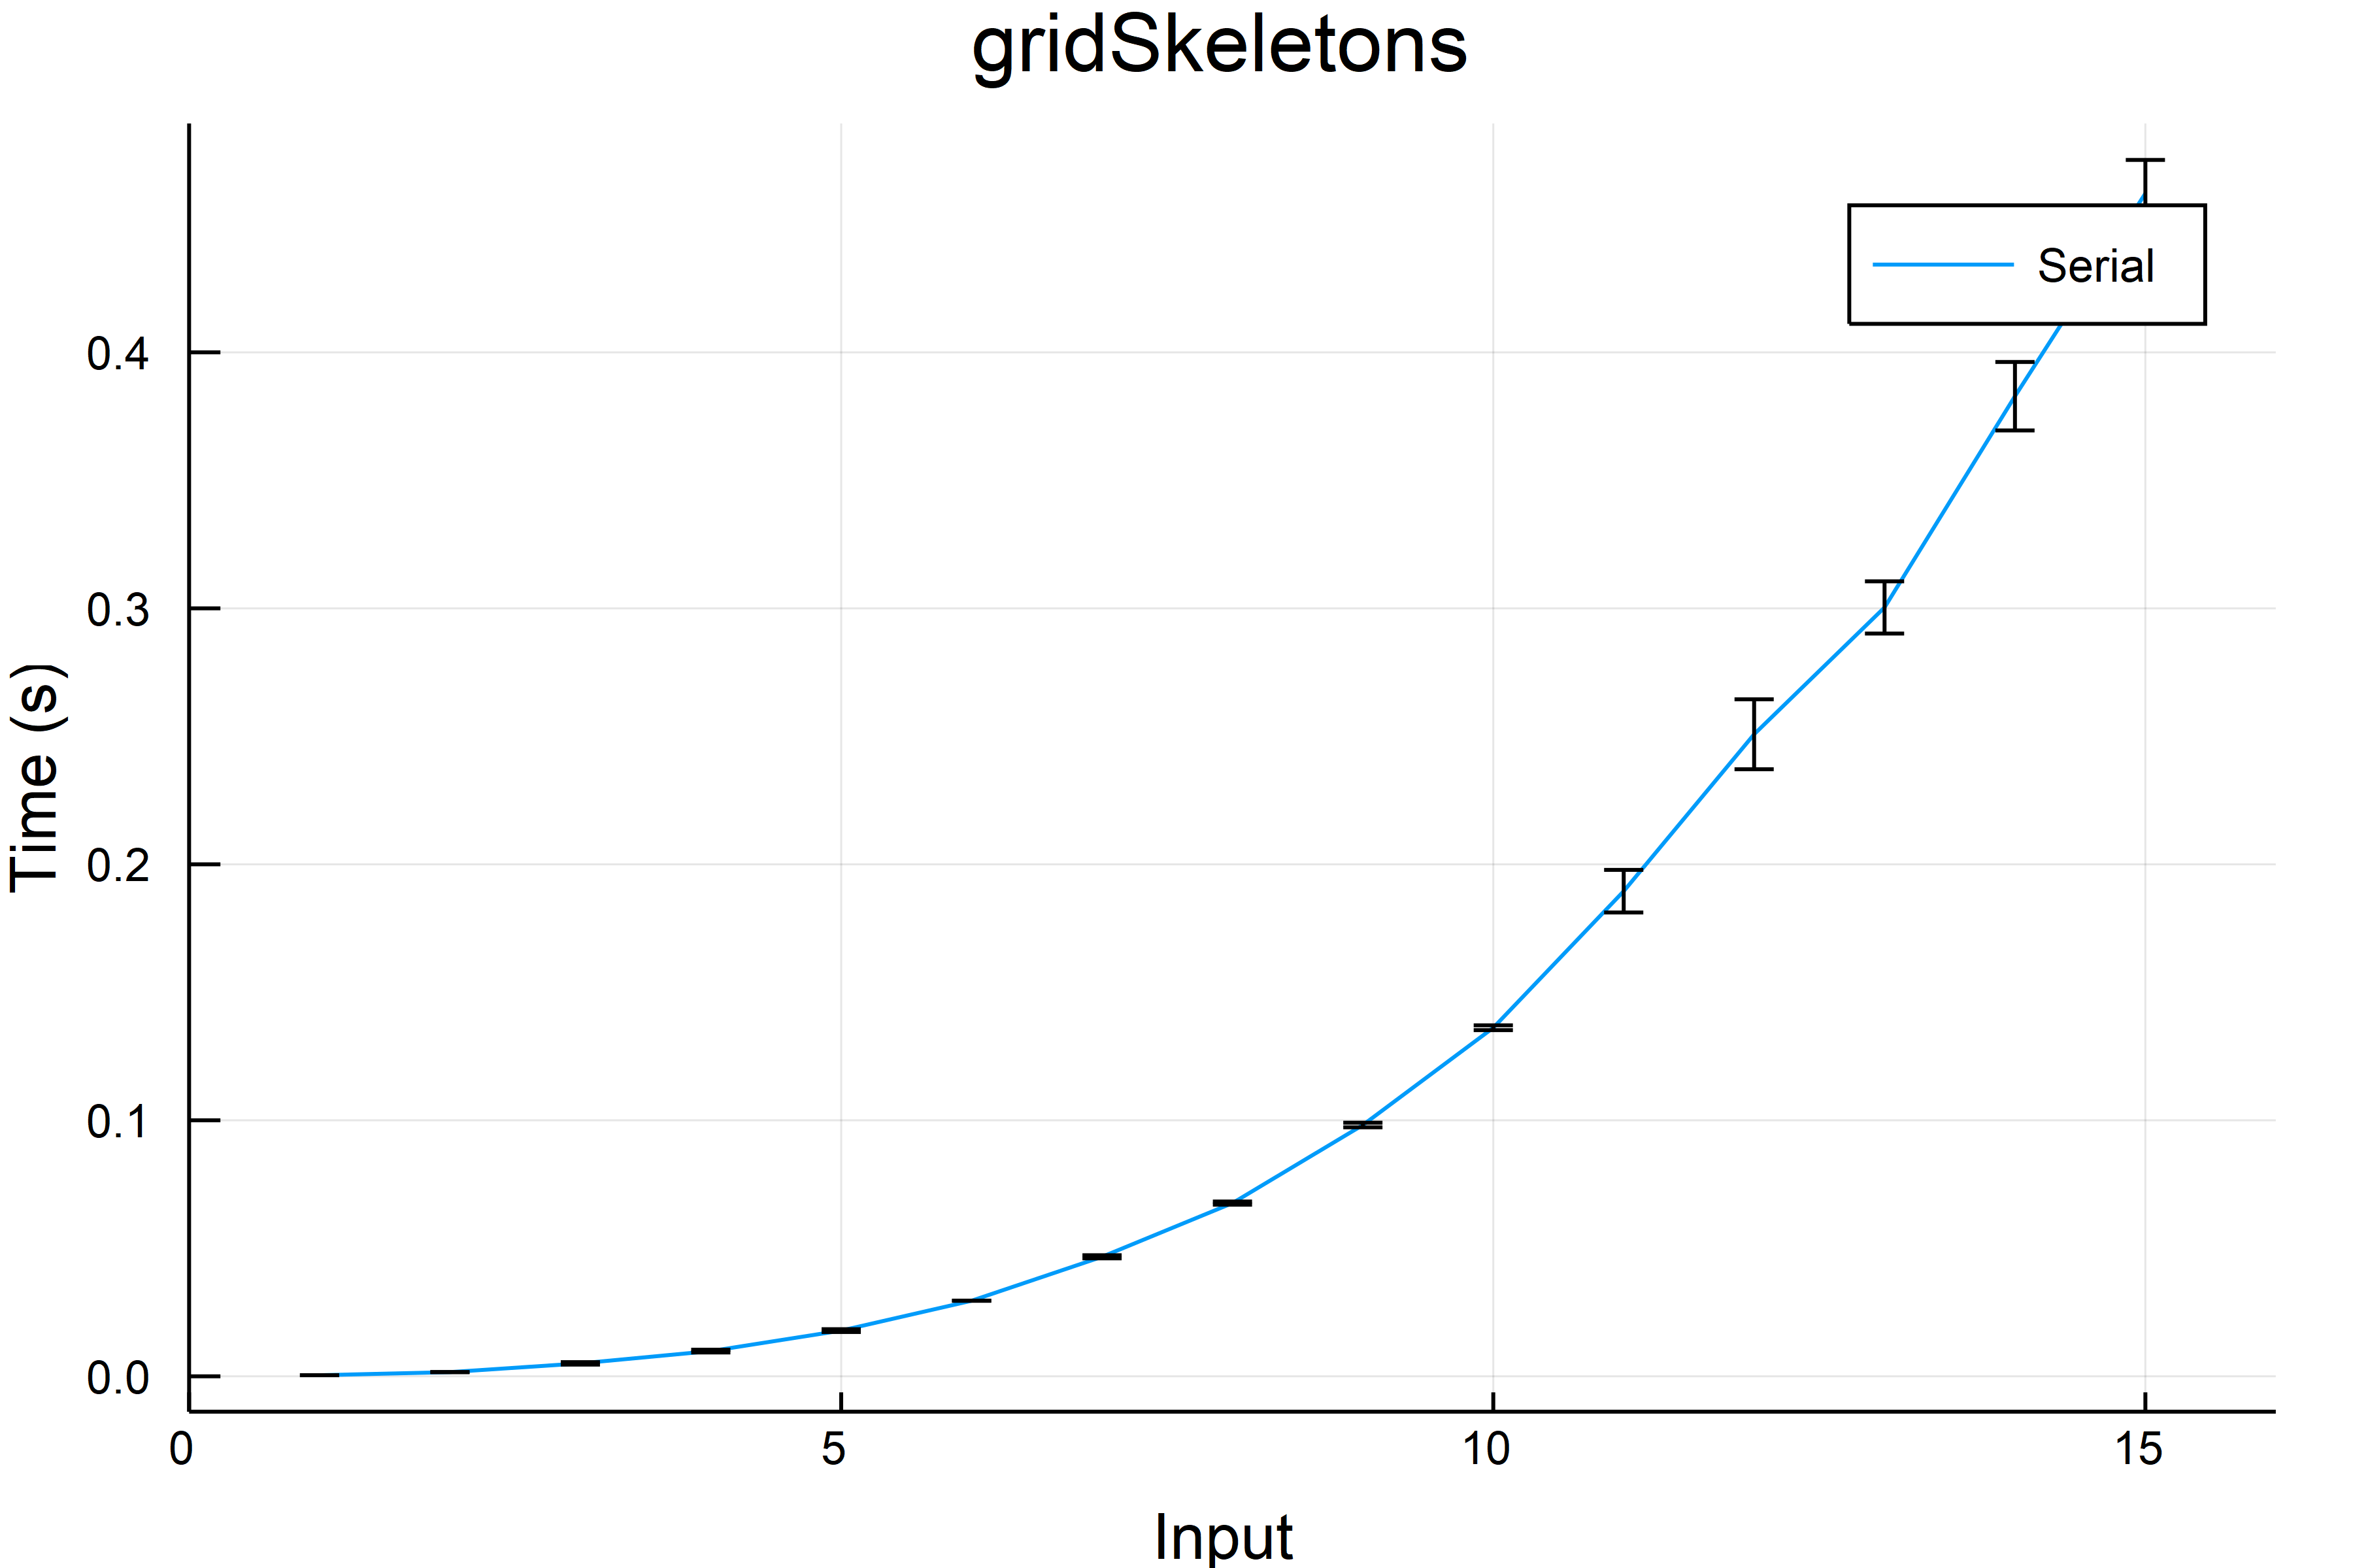
\includegraphics[scale=0.06]{gridSkeletonsSer.png}
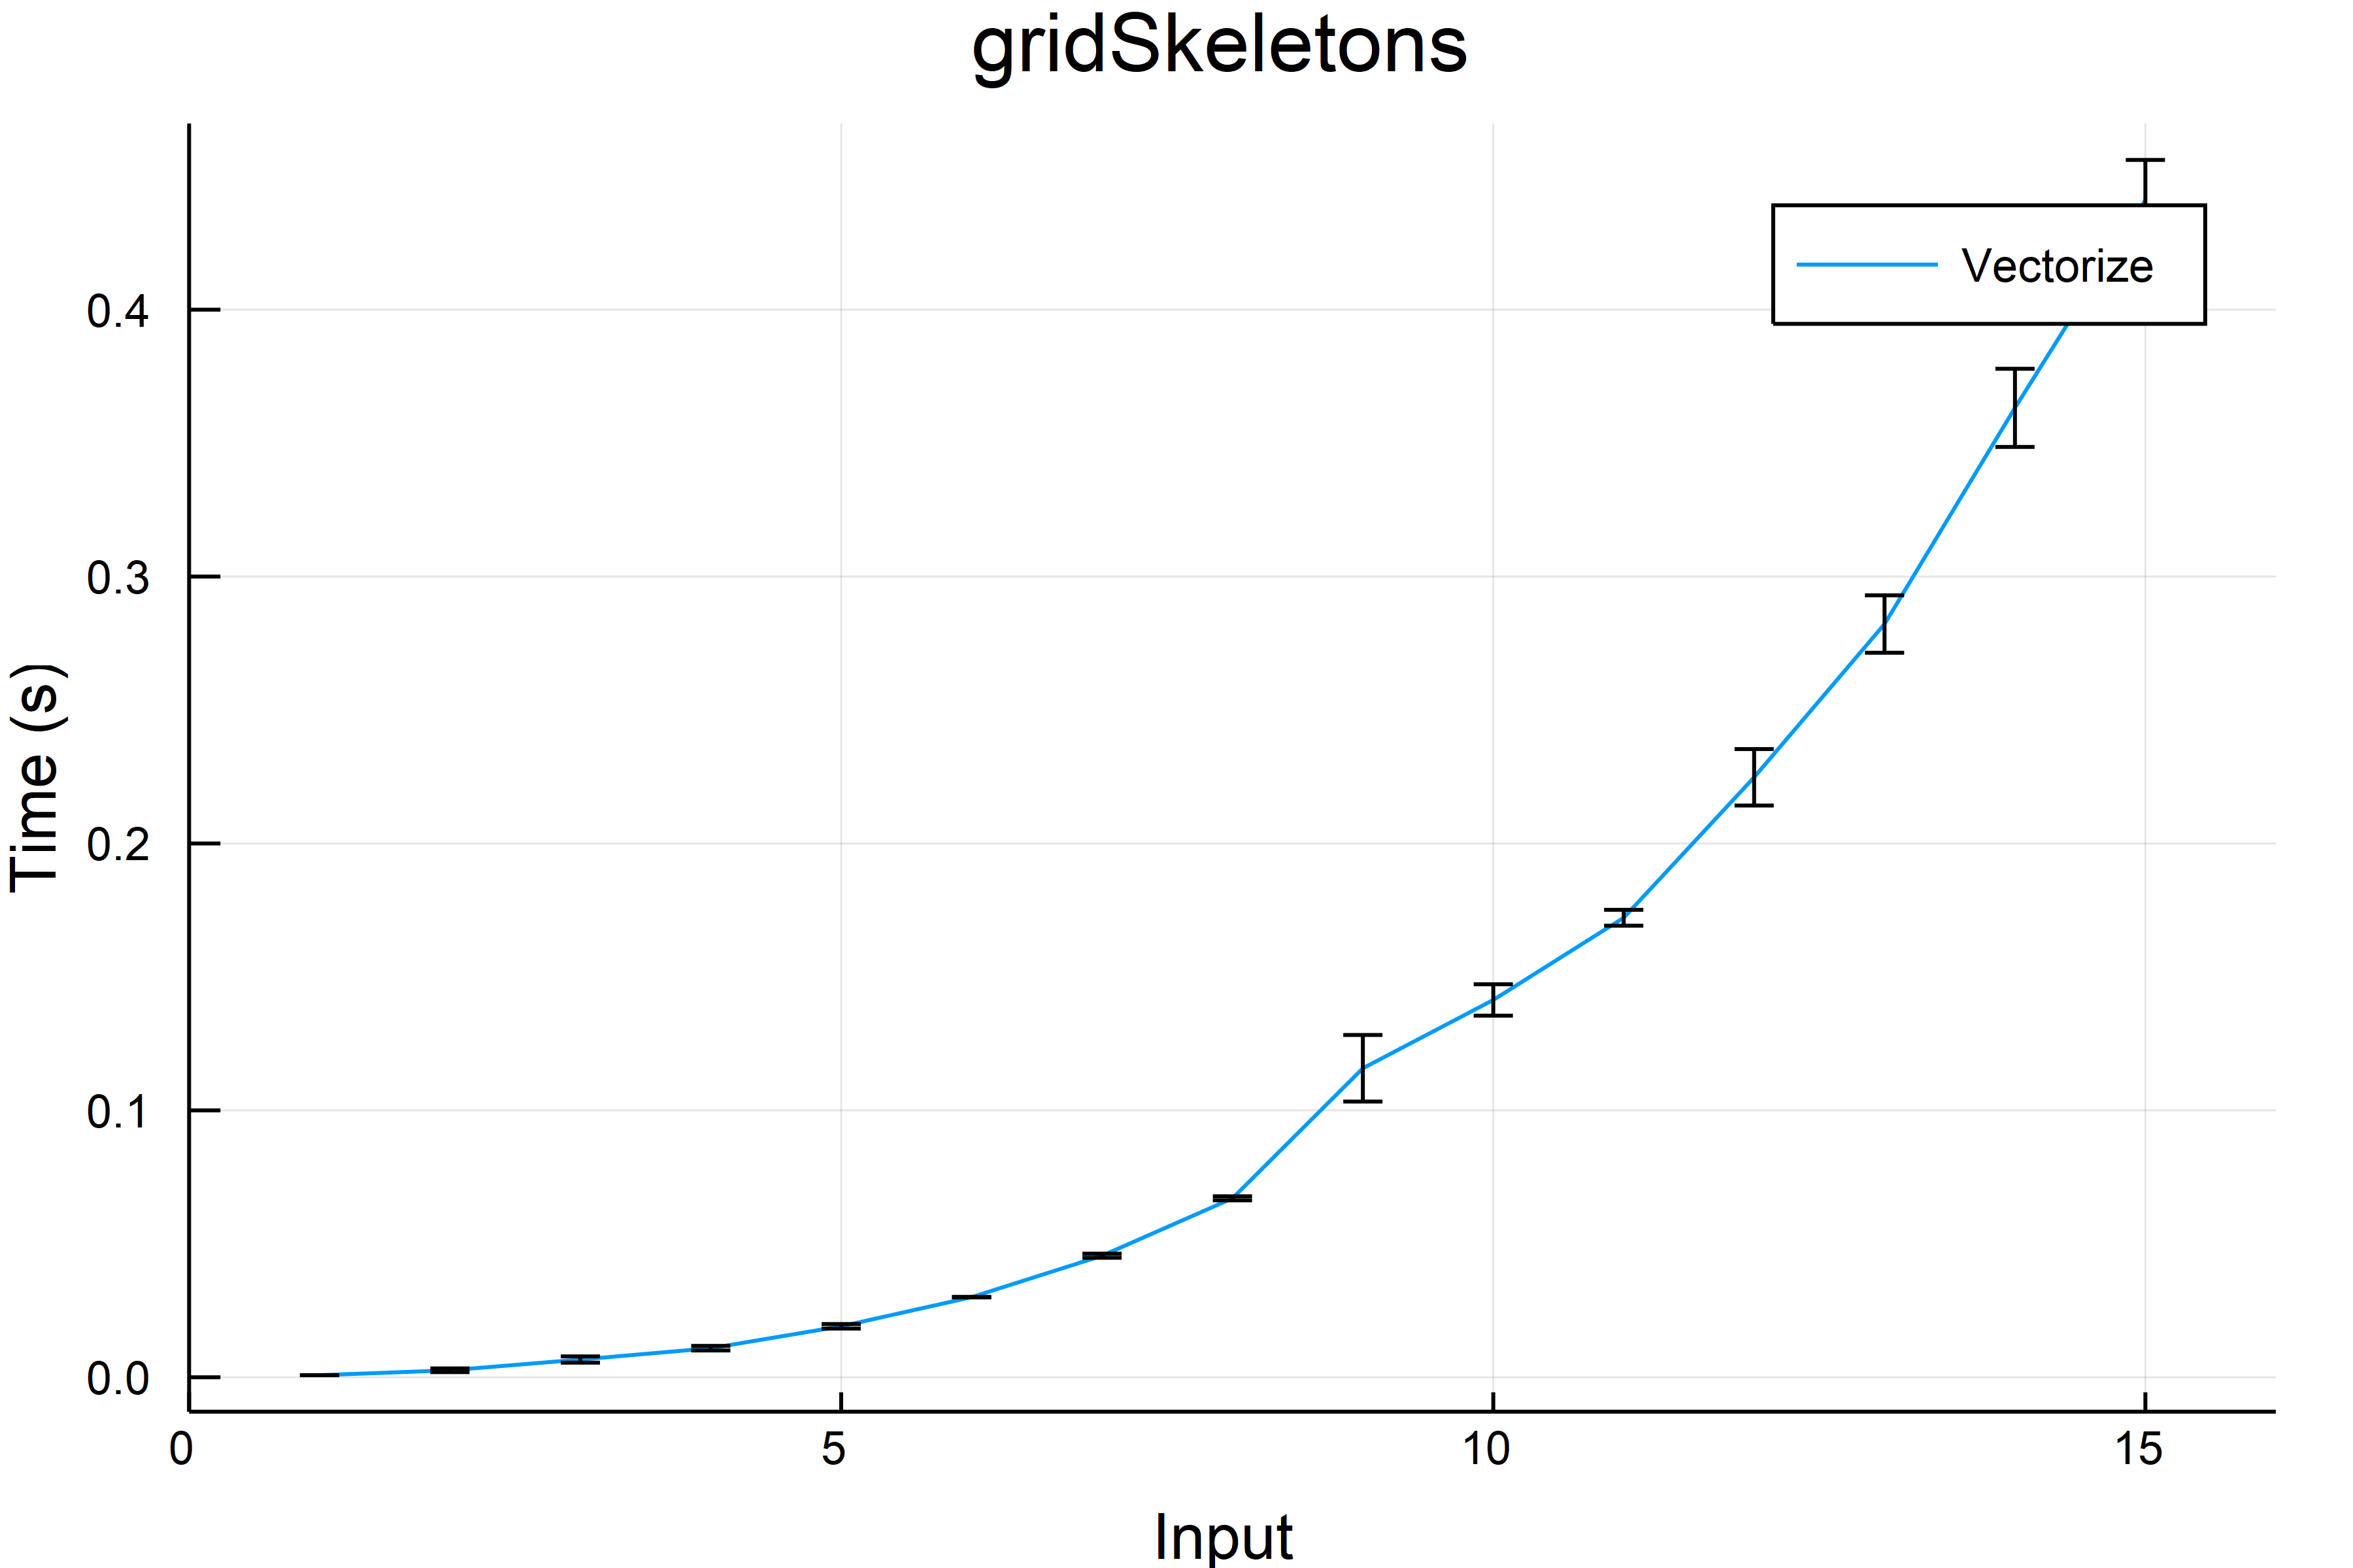
\includegraphics[scale=0.06]{gridSkeletonsVec.png}
\end{figure}

\paragraph{Compare}
\begin{flushleft}\small
\begin{list}{}{} \item
    \begin{Verbatim}[tabsize=4]
x=[xs,xv]
y=[ys,yv]

plot(x,y,yaxis="Time (s)",xlims = (0,length(datav)+1), xaxis="Input", title="gridSkeletons",
                                                    label=["Serial" "Vectorize" "Parallel"],lw=1)
   \end{Verbatim}
\end{list}
\end{flushleft}  

\begin{figure}[h!]
\centering
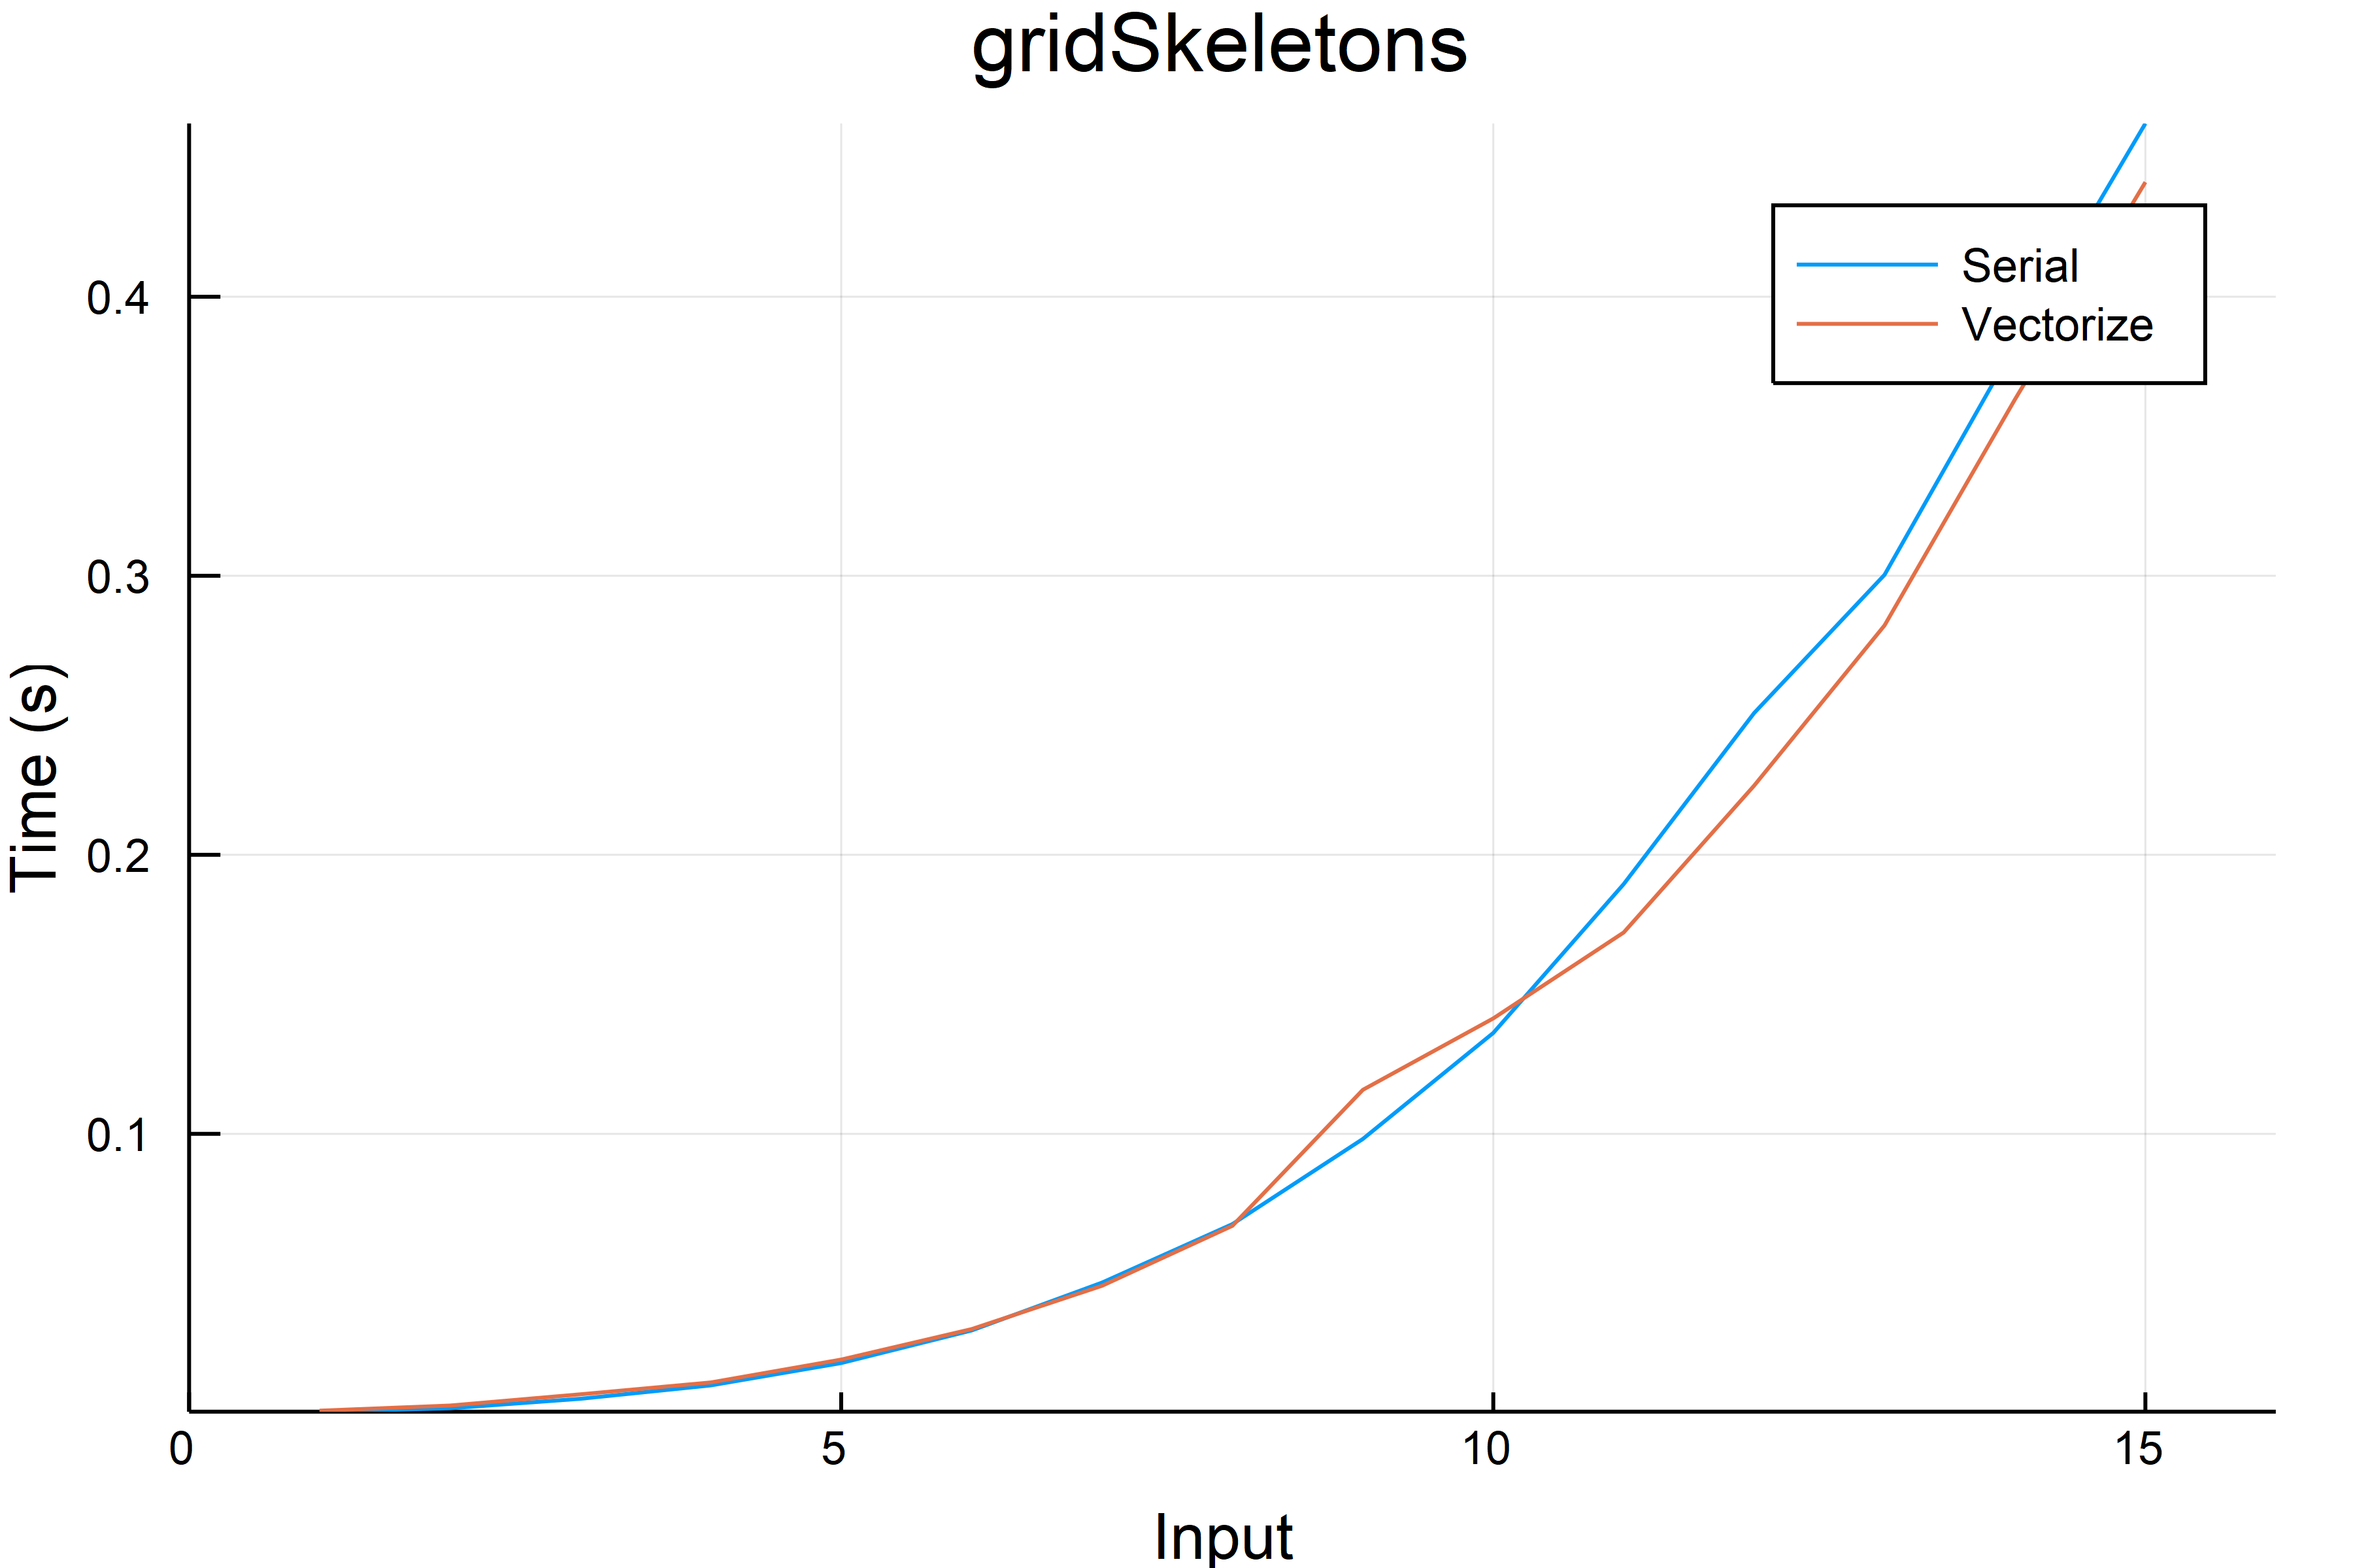
\includegraphics[scale=0.06]{gridSkeletonsCom1.png}
\end{figure}

\paragraph{Parallel}
\begin{flushleft}\small
\begin{list}{}{} \item
    \begin{Verbatim}[tabsize=4]
datap=[Time(N,pgridSkeletons,[j,j,j]) for j in range(1,6)]

xp=[1:length(datap);]
yp=mean.(datap)
yerrp=std.(datap)/sqrt(N)

plot(xp,yp,yaxis="Time (s)",xlims = (0,length(datap)+1), yerr = yerrp, xaxis="Input", 
                                            title="gridSkeletons",label=["Parallel"],lw=1)
    \end{Verbatim}
\end{list}
\end{flushleft}

\begin{figure}[h!]
\centering
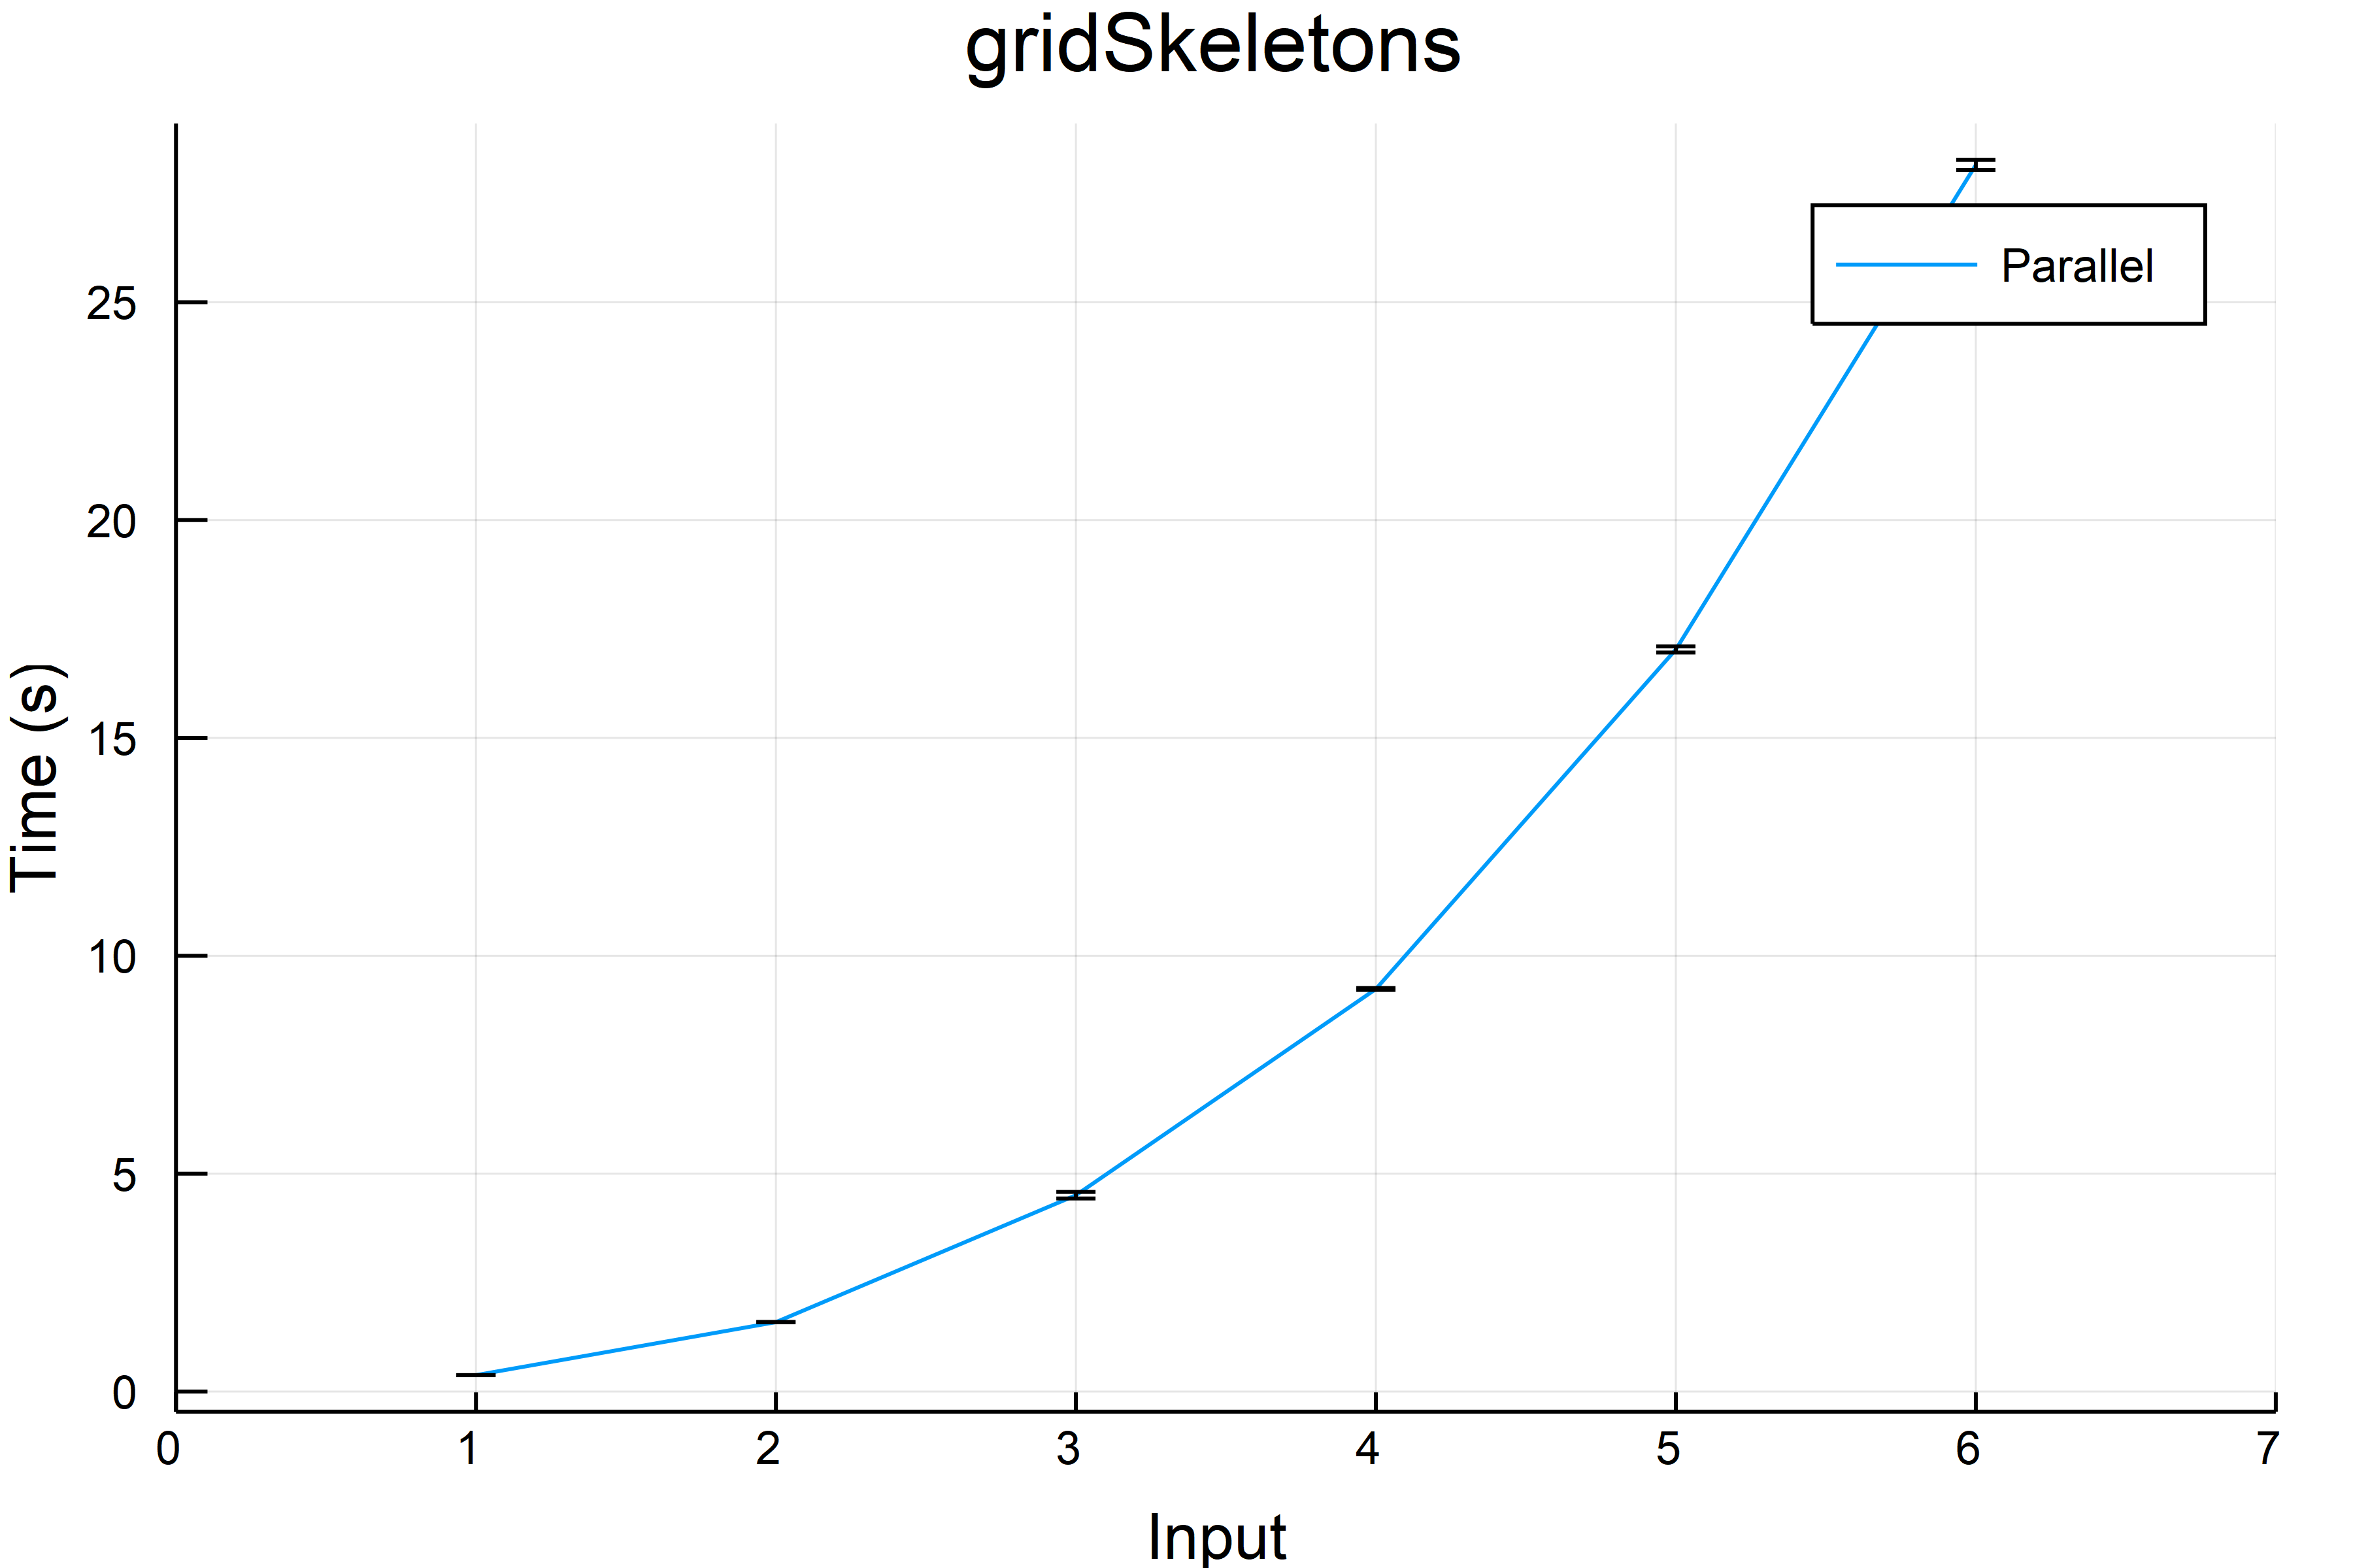
\includegraphics[scale=0.06]{gridSkeletonsPar.png}
\end{figure}

\paragraph{Compare}
\begin{flushleft}\small
\begin{list}{}{} \item
    \begin{Verbatim}[tabsize=4]
x=[xs,xv,xp]
y=[ys,yv,yp]
plot(x,y,yaxis="Time (s)",xlims = (0,length(datav)+1), xaxis="Input", title="gridSkeletons",
                                                    label=["Serial" "Vectorize" "Parallel"],lw=1)
    \end{Verbatim}
\end{list}
\end{flushleft}   

\begin{figure}[h!]
\centering
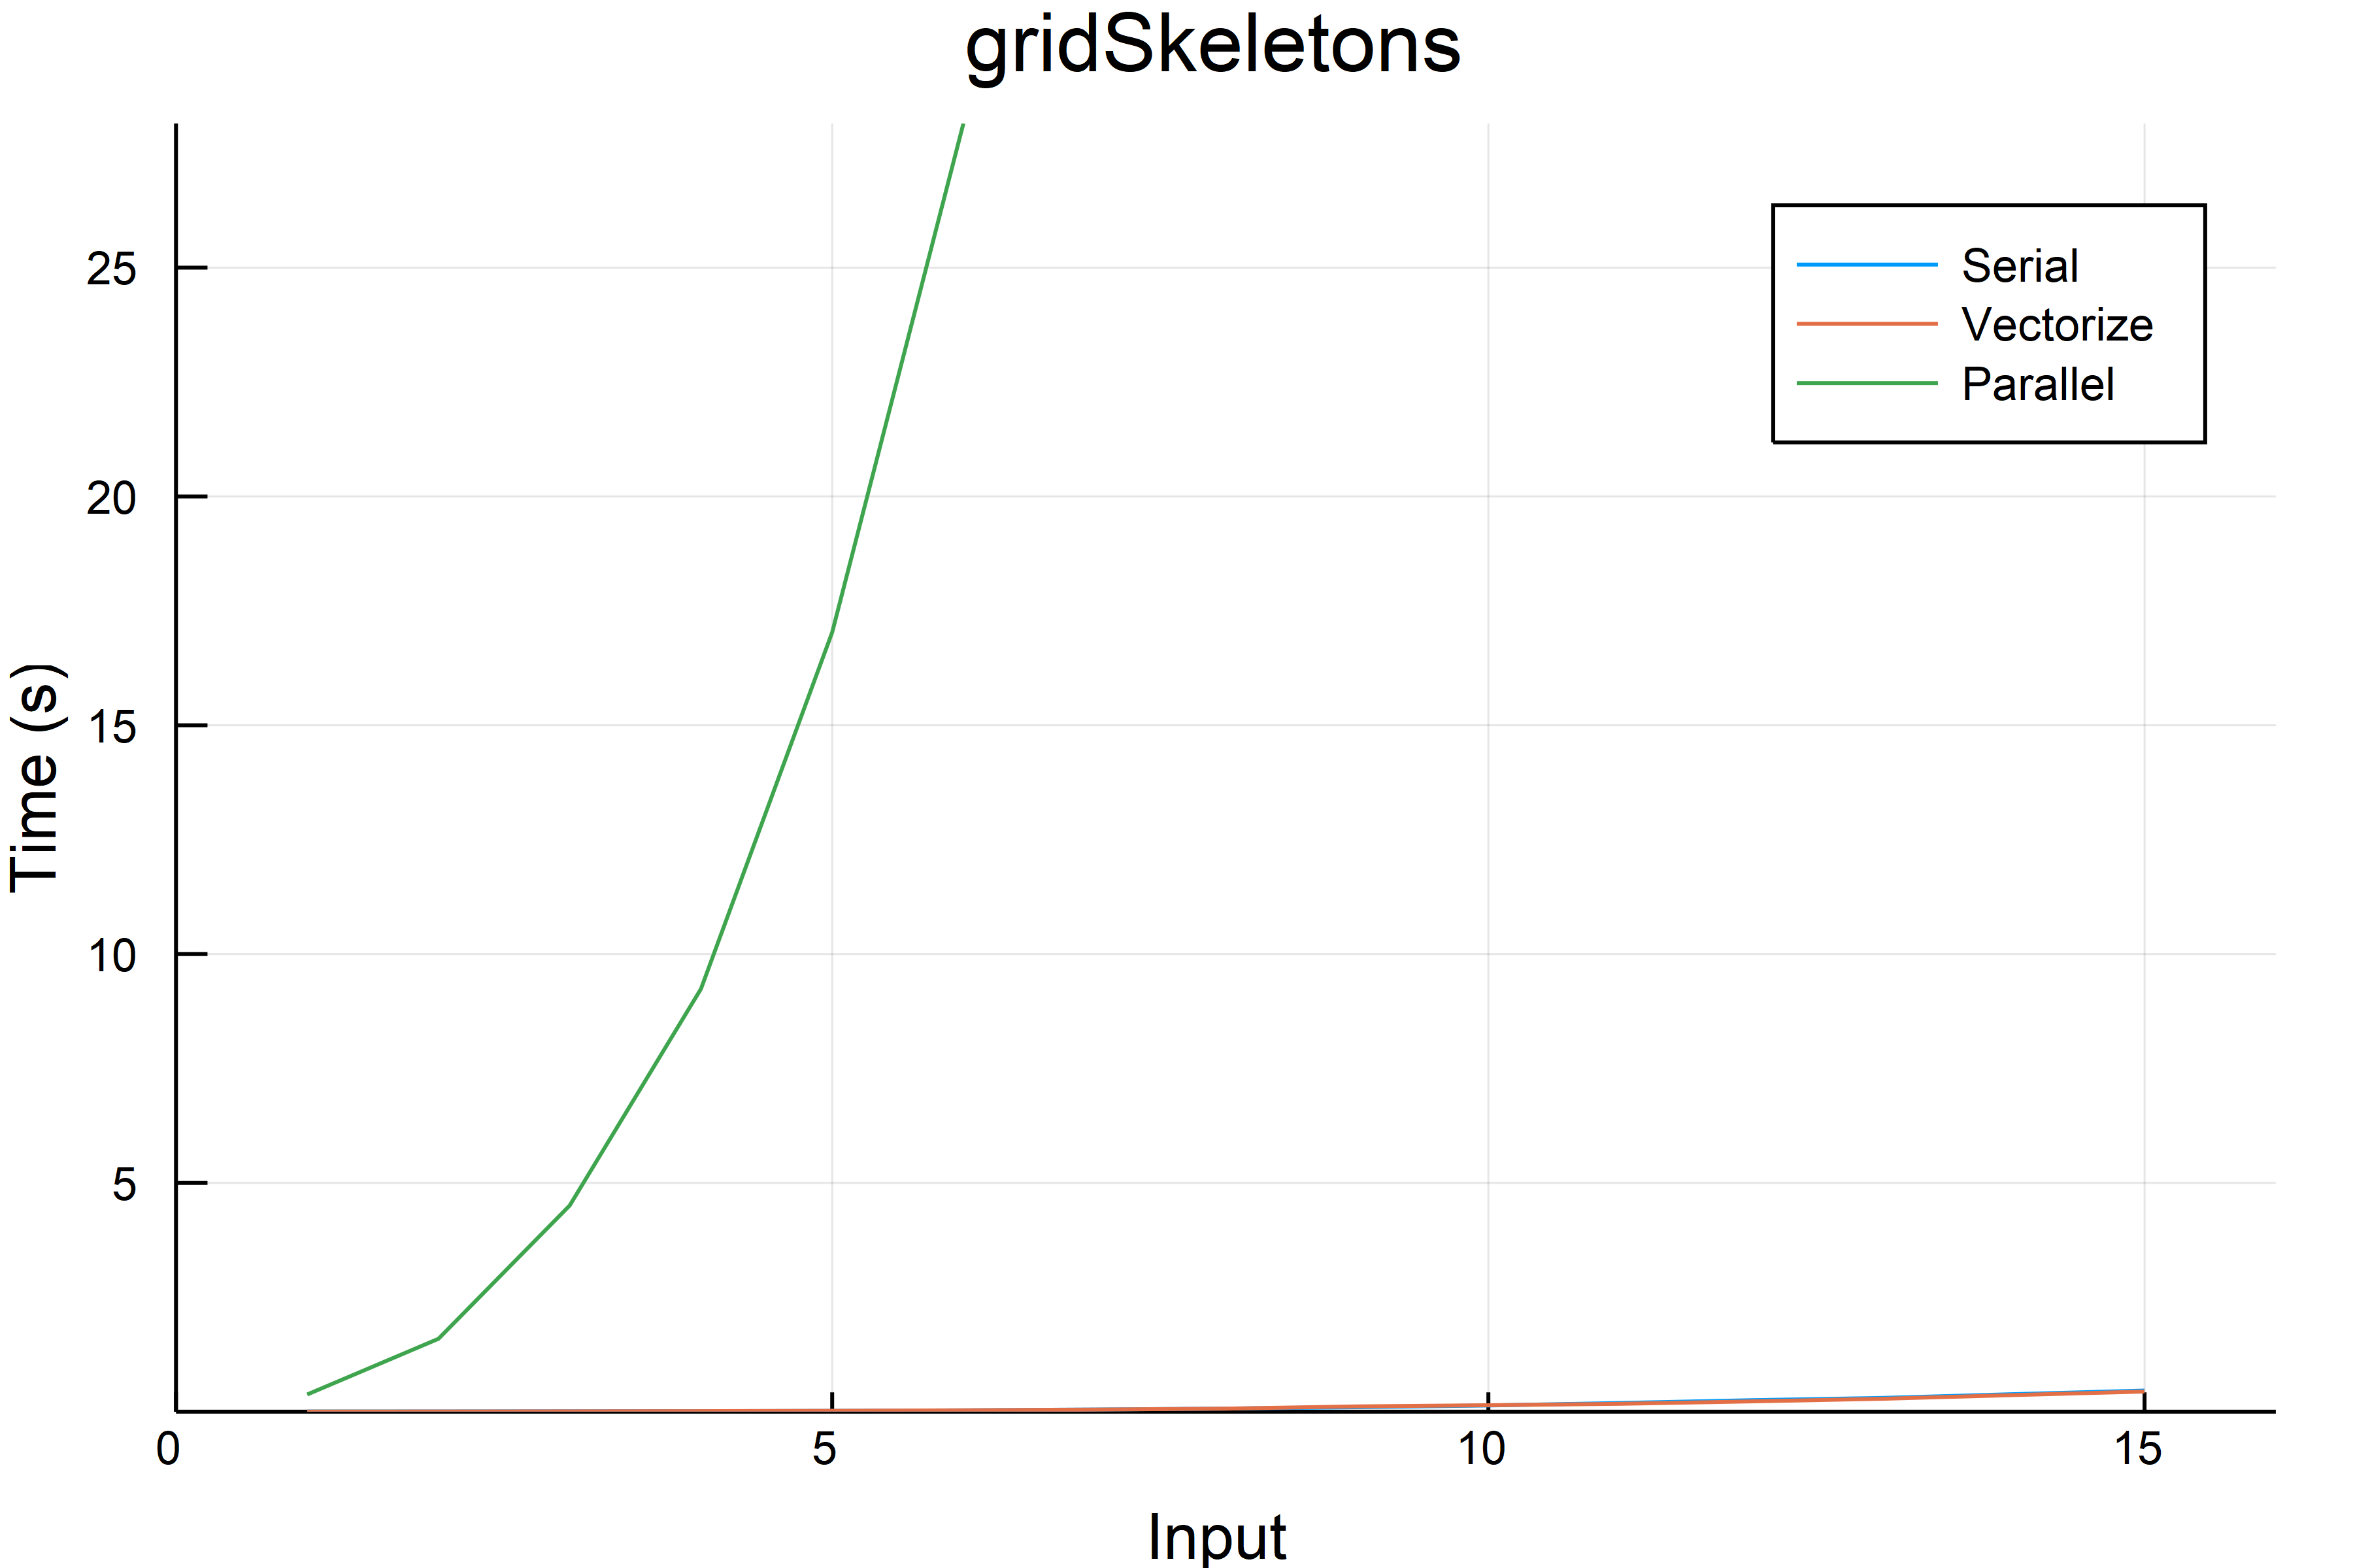
\includegraphics[scale=0.06]{gridSkeletonsCom.png}
\end{figure}
%-----------------------------------------------------------------
\section{Examples}







To view the cellular compleces, you have to import the following functions:

\begin{flushleft}\small
\begin{list}{}{}\item
\begin{Verbatim}[tabsize=4]
using PyCall
@pyimport larlib as p

function array2list(cells) 
	return PyObject([Any[cell[h] for h=1:length(cell)] for cell in cells])
end

function doublefirst(cells)
	return p.AL([cells[1],cells])
end


function lar2hpc(V::Array{Any,1},CV::Array{Any,1})
	V = hcat(V[1],V...)
	W = [Any[V[h,k] for h=1:size(V,1)] for k=1:size(V,2)]
	hpc = p.STRUCT(p.MKPOLS(PyObject([W,CV,[]])))
end

function lar2hpc(V::Array{Float64,2},CV::Array{Array{Int,1},1})
	V = hcat(V[:,1],[V[:,k] for k in 1:size(V,2)]...)
	W = [Any[V[h,k] for h=1:size(V,1)] for k=1:size(V,2)]
	hpc = p.STRUCT(p.MKPOLS(PyObject([W,CV,[]])))
end
	
function lar2hpc(V::Array{Int64,2},CV::Array{Array{Int,1},1})
	V = hcat(V[:,1],[V[:,k] for k in 1:size(V,2)]...)
	W = [Any[V[h,k] for h=1:size(V,1)] for k=1:size(V,2)]
	hpc = p.STRUCT(p.MKPOLS(PyObject([W,CV,[]])))
end

function VIEW(mod)
	V,CV= mod
	p.VIEW(lar2hpc(V,CV))
end

function lar2exploded_hpc(V::Array{Any,1},CV::Array{Any,1})
	V = hcat(V[1],V...)
	W = [Any[V[h,k] for h=1:size(V,1)] for k=1:size(V,2)]
	sx,sy,sz = 1.2,1.2,1.2
	hpc = p.EXPLODE(sx,sy,sz)(p.MKPOLS(PyObject([W,CV,[]])))
end

	
function lar2exploded_hpc(V::Array{Any,2},CV::Array{Any,2})
	Z = hcat(V[:,1],V)
	W = [Any[Z[h,k] for h=1:size(Z,1)] for k=1:size(Z,2)]
	CV = hcat(CV'...)
	CW = [Any[CV[h,k] for h=1:size(CV,1)] for k=1:size(CV,2)]
	sx,sy,sz = 1.2,1.2,1.2
	hpc = p.EXPLODE(sx,sy,sz)(p.MKPOLS(PyObject([W,CV,[]])))
	hpc = hpc
end

	
function lar2exploded_hpc(V::Array{Int64,2},CV::Array{Array{Int64,1},1})
	Z = hcat(V[:,1],V)
	W = [Any[Z[h,k] for h=1:size(Z,1)] for k=1:size(Z,2)]
	CW = [Any[cell[h] for h=1:length(cell)] for cell in CV]
	sx,sy,sz = 1.2,1.2,1.2
	hpc = p.EXPLODE(sx,sy,sz)(p.MKPOLS(PyObject([W,CV,[]])))
end

	
function lar2exploded_hpc(V::Array{Float64,2},CV::Array{Array{Int64,1},1})
	Z = hcat(V[:,1],V)
	W = [Any[Z[h,k] for h=1:size(Z,1)] for k=1:size(Z,2)]
	CW = [Any[cell[h] for h=1:length(cell)] for cell in CV]
	sx,sy,sz = 1.2,1.2,1.2
	hpc = p.EXPLODE(sx,sy,sz)(p.MKPOLS(PyObject([W,CV,[]])))
end
	
function VIEW_EXPLODE(mod)
	V,CV= mod
	p.VIEW(lar2exploded_hpc(V,CV))
end

function lar2numbered_hpc(larmodel,scaling=1.0)
	V,cells = larmodel
	VV,EV,FV,CV = cells
	Z = hcat(V[:,1],V)
	W = PyCall.PyObject([Any[Z[h,k] for h=1:size(Z,1)] for k=1:size(Z,2)])

	VV,EV,FV,CV = map(doublefirst, [VV+1,EV+1,FV+1,CV+1])
	WW,EW,FW,CW = map(array2list,[VV,EV,FV,CV])
	PyCall.PyObject([WW,EW,FW,CW])
	wire = p.MKPOL(PyCall.PyObject([W,EW,[]]))

	VV,EV,FV,CV = VV-1,EV-1,FV-1,CV-1
	WW,EW,FW,CW = map(array2list,[VV,EV,FV,CV])
	hpc = p.larModelNumbering(1,1,1)(W,PyCall.PyObject([WW,EW,FW,CW]),wire,scaling)
end


function VIEW_NUMBERED(larmodel,scaling=1.0) 
	p.VIEW(lar2numbered_hpc(larmodel,scaling))
end

\end{Verbatim}
\end{list}
\end{flushleft}
\vspace{2ex}
This function \texttt{GRID}, similar to \texttt{larGrid}, is usefull to create model because returns the right type of output can be used in LAR model.

\begin{flushleft} \small
\begin{list}{}{} \item
   \begin{Verbatim}[tabsize=4]
function GRID(n)
    function GRID1(d)
        if d==0 
            return [[i] for i in range(1,n+1)]
        elseif d==1 
            return [[i,i+1] for i in range(1,n)] 
        end
    end
    return GRID1
end
   \end{Verbatim}
\end{list}
\end{flushleft}
\paragraph{Generations, and views, of squares and cubes via Cartesian product}

\begin{flushleft} \small
\begin{list}{}{} \item
 \begin{Verbatim}[tabsize=4]
Input: mod_1 = larSplit(1)(1), GRID(1)(1)
Output: ([0.0 1.0], Array{Int64,1}[[1, 2]])

Input: square = larModelProduct(mod_1,mod_1)
Output: ([0.0 0.0 1.0 1.0; 0.0 1.0 0.0 1.0], Array{Int64,1}[[1, 2, 3, 4]])

Input: cube = larModelProduct(square,mod_1)
Output: ([0.0 0.0 … 1.0 1.0; 0.0 0.0 … 1.0 1.0; 0.0 1.0 … 0.0 1.0],
        Array{Int64,1}[[1, 2, 3, 4, 5, 6, 7, 8]])

Input: VIEW(square) 
Input: VIEW(cube) 
   \end{Verbatim}
\end{list}
\end{flushleft}

\begin{figure}[h!]
\centering
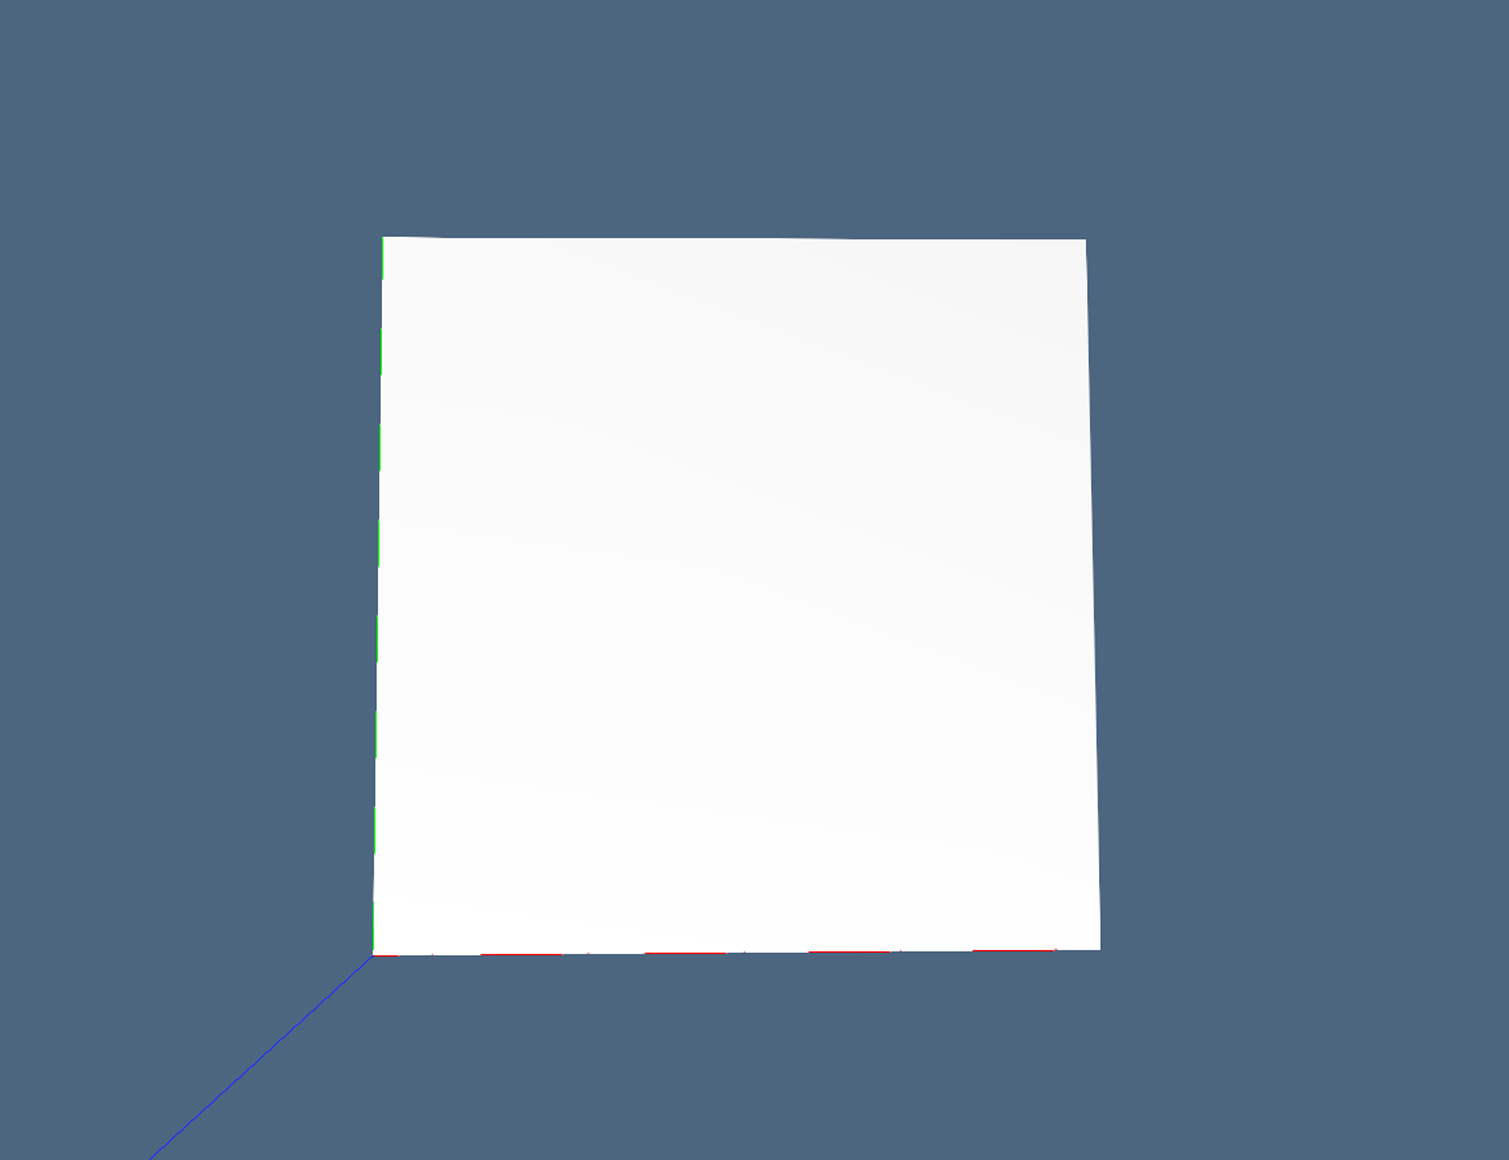
\includegraphics[scale=0.5]{quadrato.jpg}
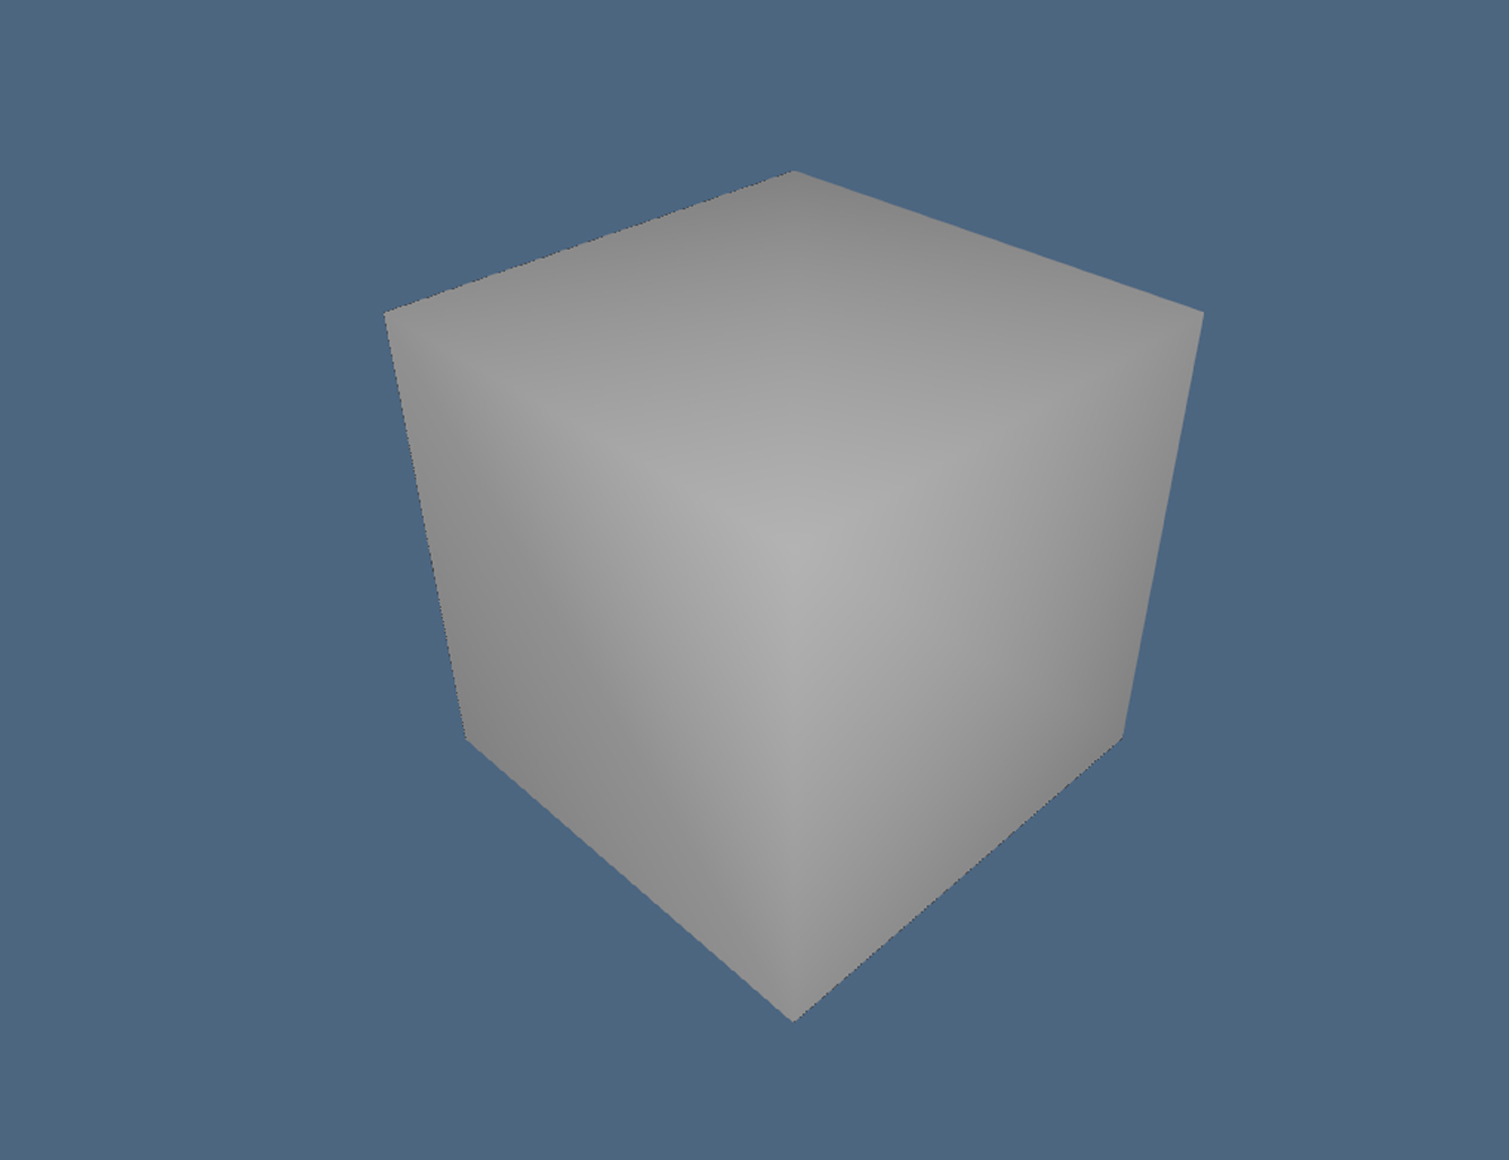
\includegraphics[scale=0.5]{cubo.jpg}
\caption{Square and Cube}
\end{figure}
\newpage
\paragraph{Extration of facets with larCuboidsFacets}
\begin{flushleft} \small
\begin{list}{}{} \item
   \begin{Verbatim}[tabsize=4]
Input: CUBE=larCuboids([1,1,1])
Output: ([0 0 … 1 1; 0 0 … 1 1; 0 1 … 0 1], Array{Int64,1}[[1, 2, 3, 4, 5, 6, 7, 8]])

Input: V,FACES=larCuboidsFacets(CUBE[1],CUBE[2])
Output: ([0 0 … 1 1; 0 0 … 1 1; 0 1 … 0 1],
        Array{Int64,1}[[1, 2, 3, 4], [1, 2, 5, 6], [1, 3, 5, 7], [2, 4, 6, 8],
        [3, 4, 7, 8], [5, 6, 7, 8]])

Input: length(FACES)
Output: 6

Input: mod_3=V,FACES
Output: ([0 0 … 1 1; 0 0 … 1 1; 0 1 … 0 1],
        Array{Int64,1}[[1, 2, 3, 4], [1, 2, 5, 6], [1, 3, 5, 7], [2, 4, 6, 8],
        [3, 4, 7, 8], [5, 6, 7, 8]])

Input: VIEW_EXPLODE(mod_3)
   \end{Verbatim}
\end{list}
\end{flushleft}

\begin{figure}[h!]
\centering
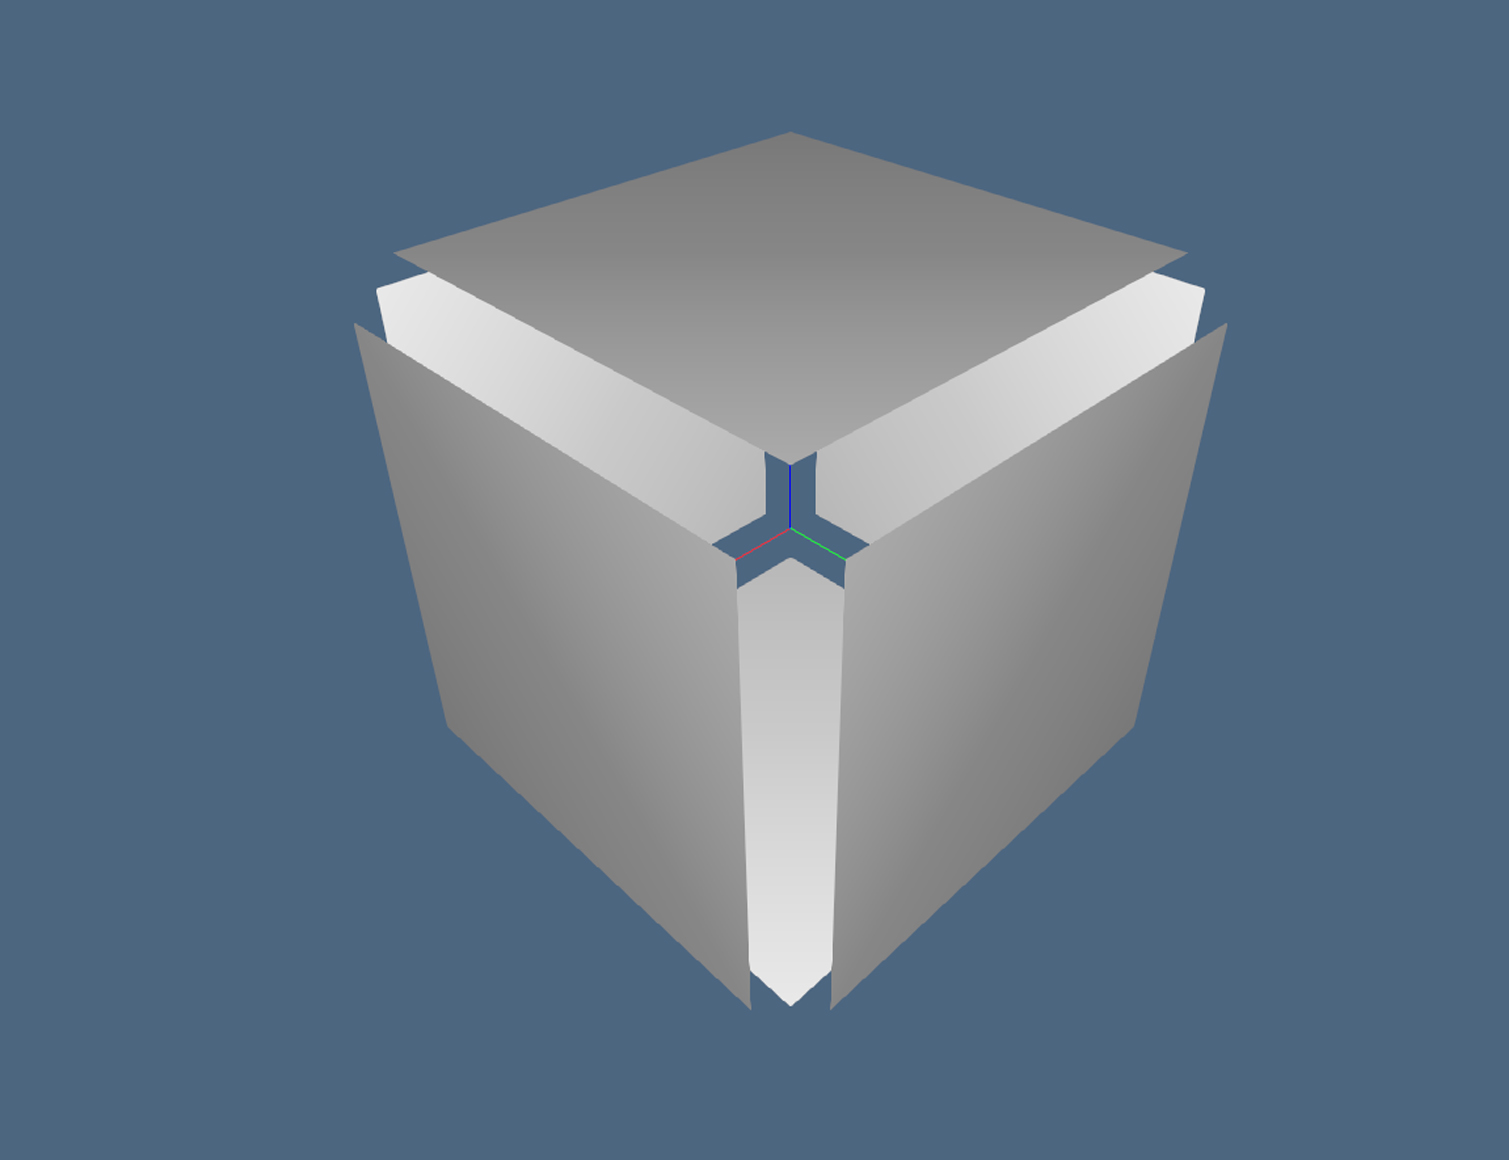
\includegraphics[scale=0.6]{estrazioneFacce.jpg}
\caption{Exploded view of facets}
\end{figure}

\paragraph{Exploded views}
\begin{flushleft} \small
\begin{list}{}{} \item
   \begin{Verbatim}[tabsize=4]
Input: mod_2 = larSplit(3)(3), GRID(3)(1)
Output: ([0.0 1.0 2.0 3.0], Array{Int64,1}[[1, 2], [2, 3], [3, 4]])

Input: squares = larModelProduct(mod_2,mod_2)
Output: ([0.0 0.0 … 3.0 3.0; 0.0 1.0 … 2.0 3.0],
        Array{Int64,1}[[1, 2, 5, 6], [2, 3, 6, 7], [3, 4, 7, 8], [5, 6, 9, 10],
        [6, 7, 10, 11], [7, 8, 11, 12], [9, 10, 13, 14], [10, 11, 14, 15], 
        [11, 12, 15, 16]])

Input: VIEW_EXPLODE(squares)

Input: cubes = larModelProduct(squares,mod_2)
Output: ([0.0 0.0 … 3.0 3.0; 0.0 0.0 … 3.0 3.0; 0.0 1.0 … 2.0 3.0],
        Array{Int64,1}[[1, 2, 5, 6, 17, 18, 21, 22],
        [2, 3, 6, 7, 18, 19, 22, 23], [3, 4, 7, 8, 19, 20, 23, 24],
        [5, 6, 9, 10, 21, 22, 25, 26], [6, 7, 10, 11, 22, 23, 26, 27], 
        [7, 8, 11, 12, 23, 24, 27, 28],[9, 10, 13, 14, 25, 26, 29, 30],
        [10, 11, 14, 15, 26, 27, 30, 31], [11, 12, 15, 16, 27, 28, 31, 32],
        [17, 18, 21, 22, 33, 34, 37, 38]  … 
        [27, 28, 31, 32, 43, 44, 47, 48], [33, 34, 37, 38, 49, 50, 53, 54],
        [34, 35, 38, 39, 50, 51, 54, 55], [35, 36, 39, 40, 51, 52, 55, 56], 
        [37, 38, 41, 42, 53, 54, 57, 58], [38, 39, 42, 43, 54, 55, 58, 59],
        [39, 40, 43, 44, 55, 56, 59, 60], [41, 42, 45, 46, 57, 58, 61, 62], 
        [42, 43, 46, 47, 58, 59, 62, 63], [43, 44, 47, 48, 59, 60, 63, 64]])


Input: vertici=size(cubes[1],2)
Output: 64

Input: cubi=length(cubes[2])
Output: 27

Input: VIEW_EXPLODE(cubes)
   \end{Verbatim}
\end{list}
\end{flushleft}

\begin{figure}[h!]
\centering
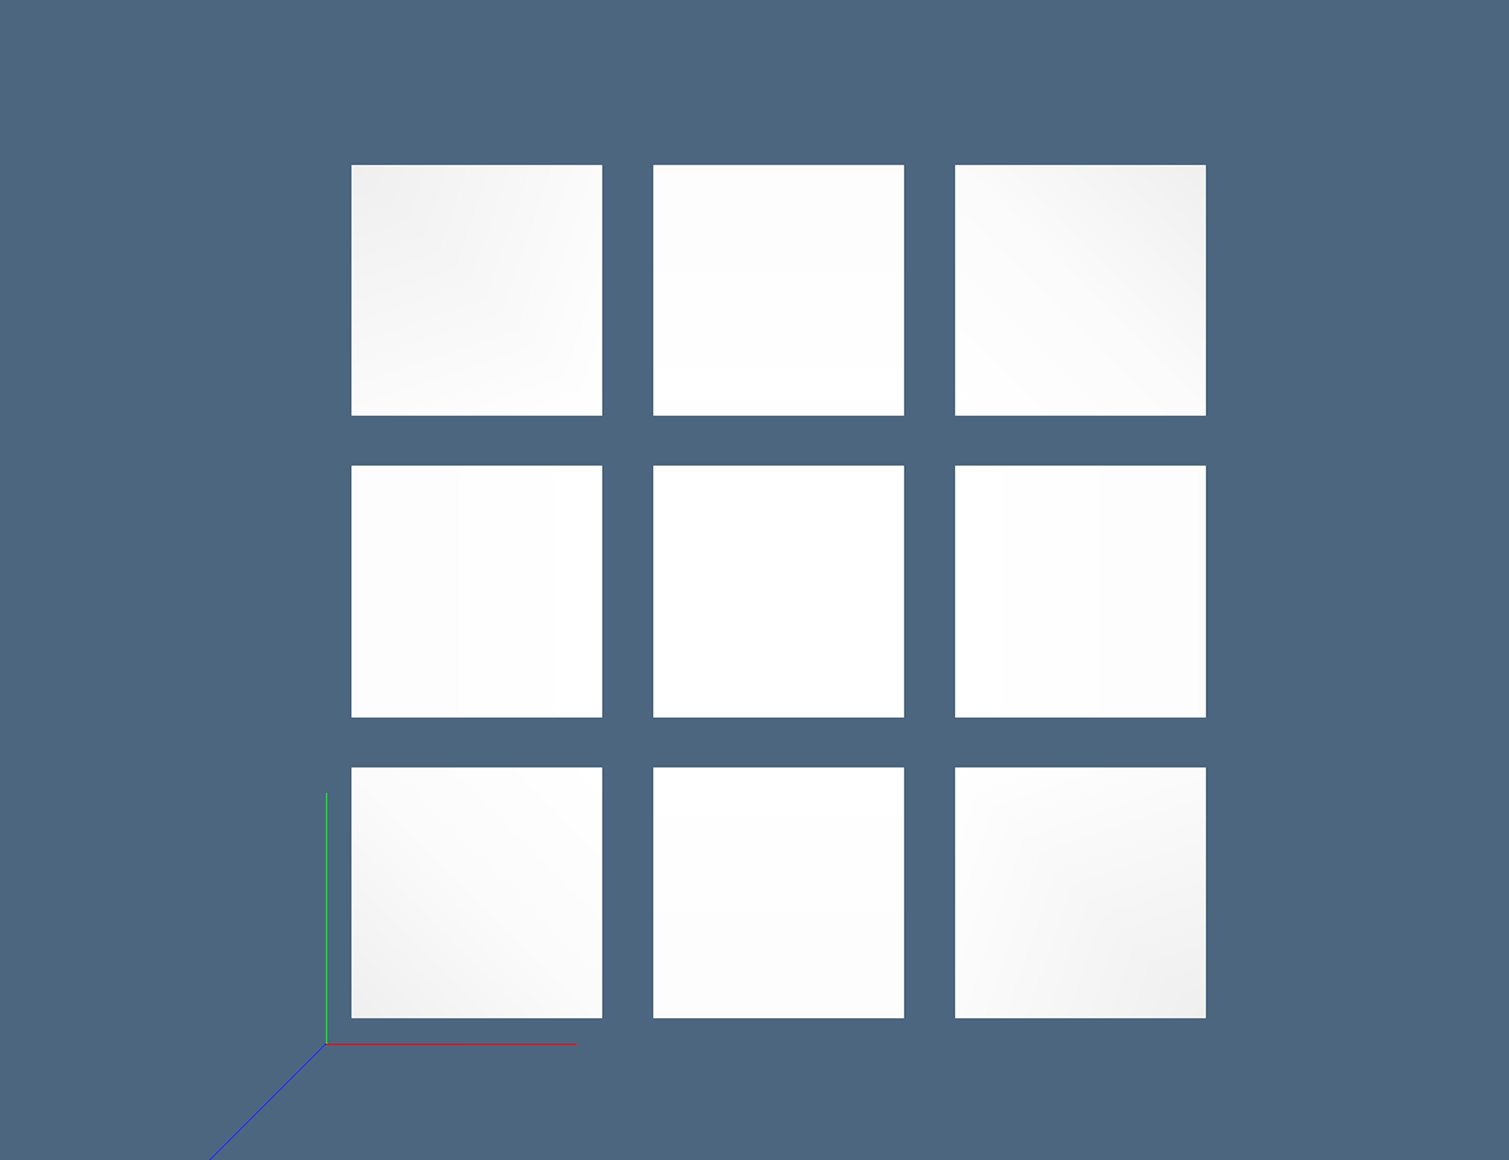
\includegraphics[scale=0.5]{celleEsplose.jpg}
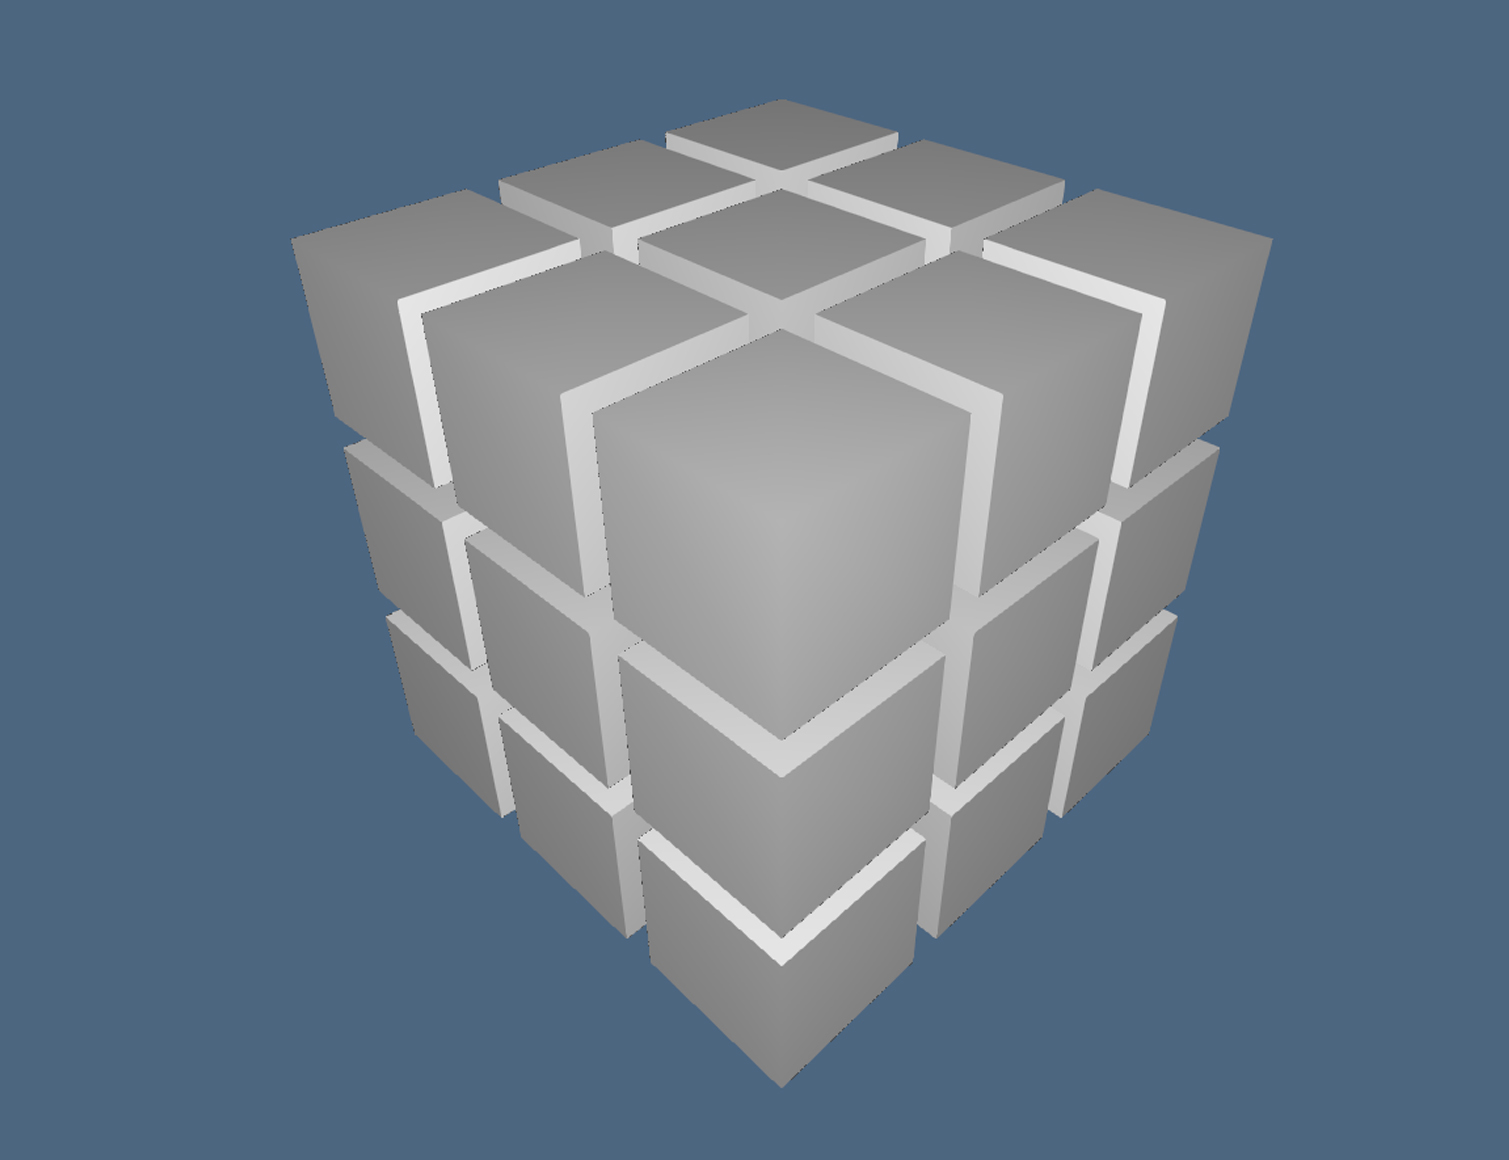
\includegraphics[scale=0.5]{celleEsplose2.jpg}
\caption{Exploded square and cube}
\end{figure}

\paragraph{View of numbered skeletons}
\begin{flushleft} \small

\begin{list}{}{} \item
   \begin{Verbatim}[tabsize=4]
Input: schel1=CUBE[1],gridSkeletons([1,1,1])
Output: ([0 0 … 1 1; 0 0 … 1 1; 0 1 … 0 1],
        Array{Array{Int64,1},1}[Array{Int64,1}[[1], [2], [3], [4], [5], [6], [7], [8]], 
        Array{Int64,1}[[1, 2], [3, 4], [5, 6], [7, 8], [1, 3], [2, 4], [5, 7],
        [6, 8], [1, 5], [2, 6], [3, 7], [4, 8]],
        Array{Int64,1}[[1, 2, 3, 4], [5, 6, 7, 8], [1, 2, 5, 6], [3, 4, 7, 8],
        [1, 3, 5, 7], [2, 4, 6, 8]], Array{Int64,1}[[1, 2, 3, 4, 5, 6, 7, 8]]])

Input: VIEW_NUMBERED(schel1)
   \end{Verbatim}
\end{list}
\end{flushleft}

\begin{figure}[h!]
\centering
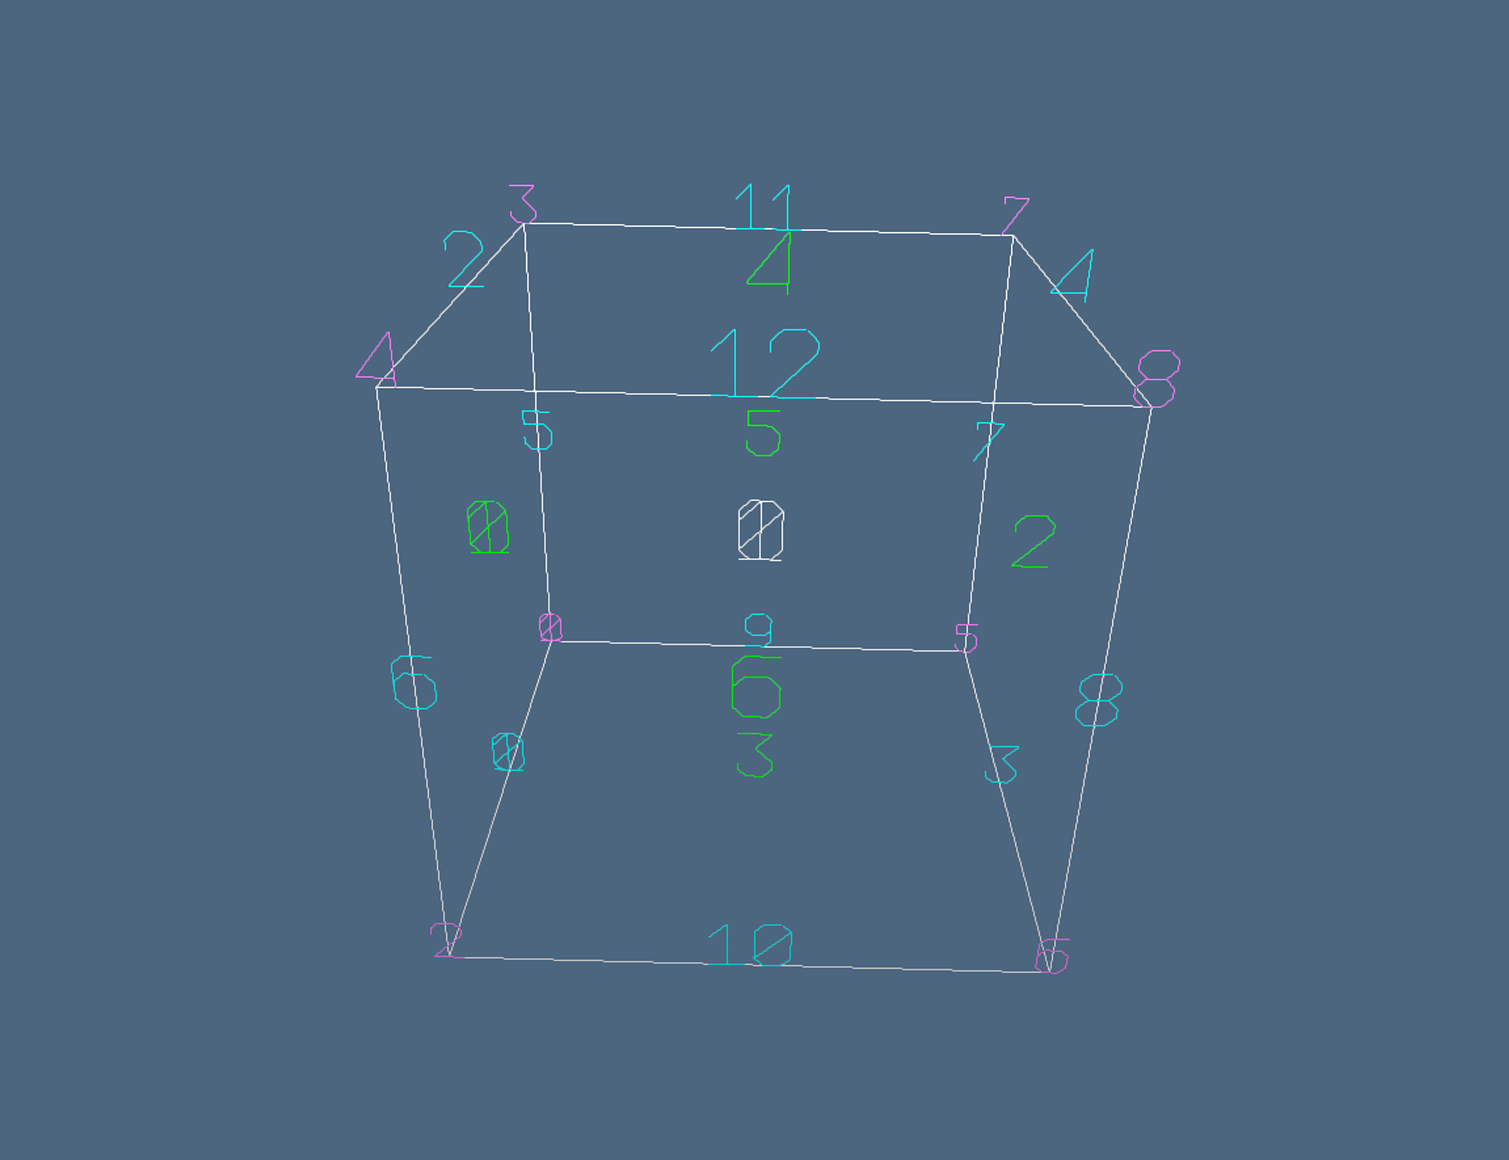
\includegraphics[scale=0.6]{numerazioneskel.jpg}
\caption{Numbered view of cube}
\end{figure}

\newpage
\paragraph{Generation and view of triangles}

\begin{flushleft} \small
\begin{list}{}{} \item
   \begin{Verbatim}[tabsize=4]
Input: v,ev=[0 1 0; 0 0 1],[[1,2],[2,3],[1,3]]
Output: ([0 1 0; 0 0 1], Array{Int64,1}[[1, 2], [2, 3], [1, 3]])

Input: tri_edge=v,ev;

Input: VIEW(tri_edge)

Input: v,fv=[0 1 0; 0 0 1],[[1,2,3]]
Output: ([0 1 0; 0 0 1], Array{Int64,1}[[1, 2, 3]])

Input: triangle=v,fv

Input: VIEW(triangle)
   \end{Verbatim}
\end{list}
\end{flushleft}

\begin{figure}[h!]
\centering
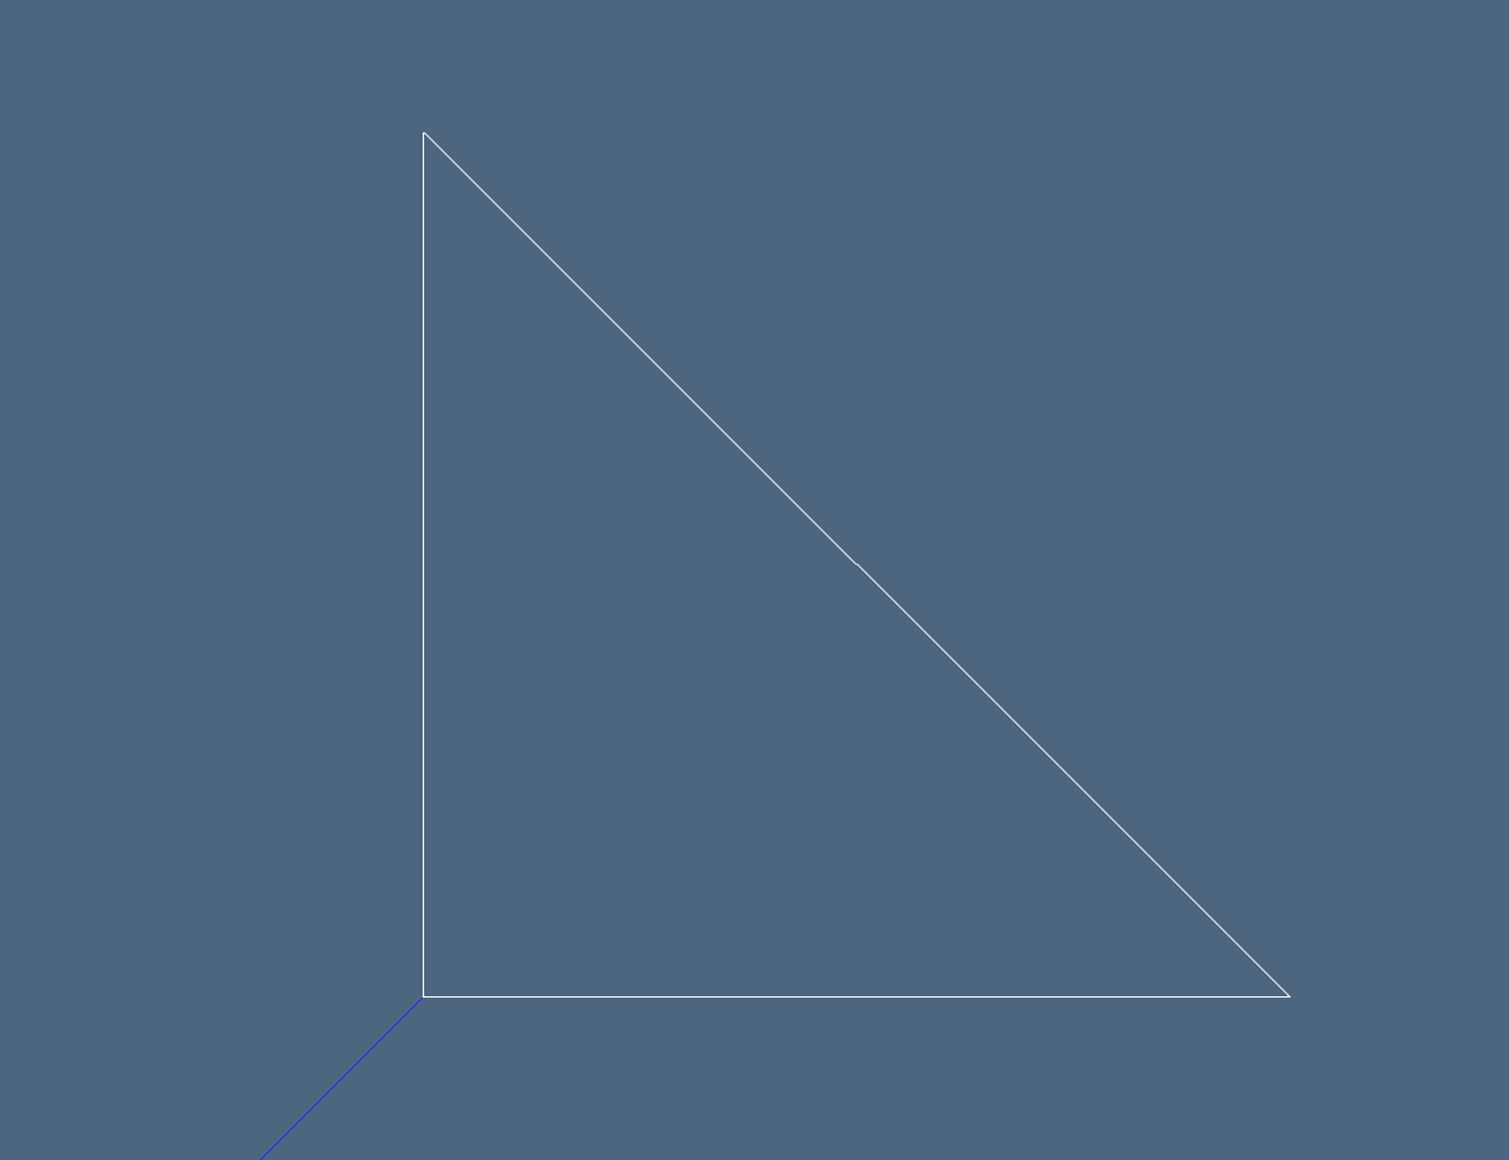
\includegraphics[scale=0.5]{triangolo.jpg}

\includegraphics[scale=0.5]{triangolo2.jpg}
\caption{View of triangle's edges and facet }
\end{figure}

\paragraph{0-,1-,2- and 3- dimensional skeletons}
\begin{flushleft} \small

\begin{list}{}{} \item
   \begin{Verbatim}[tabsize=4]
Input: vv,evv=[0 1 0 0 ; 0 0 1 0;0 0 0 1],larSimplicialStack([[1,2,3,4]])[2]
Output: ([0 1 0 0; 0 0 1 0; 0 0 0 1], Array{Int64,1}[[1, 2], [1, 3], [1, 4], [2, 3], [2, 4], [3, 4]])

Input: tetra_edge=vv,evv;
Input: VIEW(tetra_edge)

Input: vv,fvv=[0 1 0 0 ; 0 0 1 0;0 0 0 1],larSimplicialStack([[1,2,3,4]])[3]
Output: ([0 1 0 0; 0 0 1 0; 0 0 0 1], Array{Int64,1}[[1, 2, 3], [1, 2, 4], [1, 3, 4], [2, 3, 4]])

Input: tetra_face=vv,fvv;
Input: VIEW_EXPLODE(tetra_face)

Input: vv,cvv=[0 1 0 0 ; 0 0 1 0;0 0 0 1],[[1,2,3,4]];
Input: simpli=larSimplicialStack(cvv)
Output: 4-element Array{Array{Array{Int64,1},1},1}:
         Array{Int32,1}[[1], [2], [3], [4]]
         Array{Int32,1}[[1, 2], [1, 3], [1, 4], [2, 3], [2, 4], [3, 4]]
         Array{Int32,1}[[1, 2, 3], [1, 2, 4], [1, 3, 4], [2, 3, 4]]
         Array{Int32,1}[[1, 2, 3, 4]]

Input: schel2=vv,simpli
Output: (Array{Int32,1}[[1], [2], [3], [4]],
        Array{Array{Int64,1},1}[Array{Int64,1}[[1], [2], [3], [4]],
        Array{Int32,1}[[1, 2], [1, 3], [1, 4], [2, 3], [2, 4], [3, 4]],
        Array{Int32,1}[[1, 2, 3], [1, 2, 4], [1, 3, 4], [2, 3, 4]],
        Array{Int32,1}[[1, 2, 3, 4]]])

Input: VIEW_NUMBERED(schel2)
   \end{Verbatim}
\end{list}
\end{flushleft}

\begin{figure}[h!]
\centering
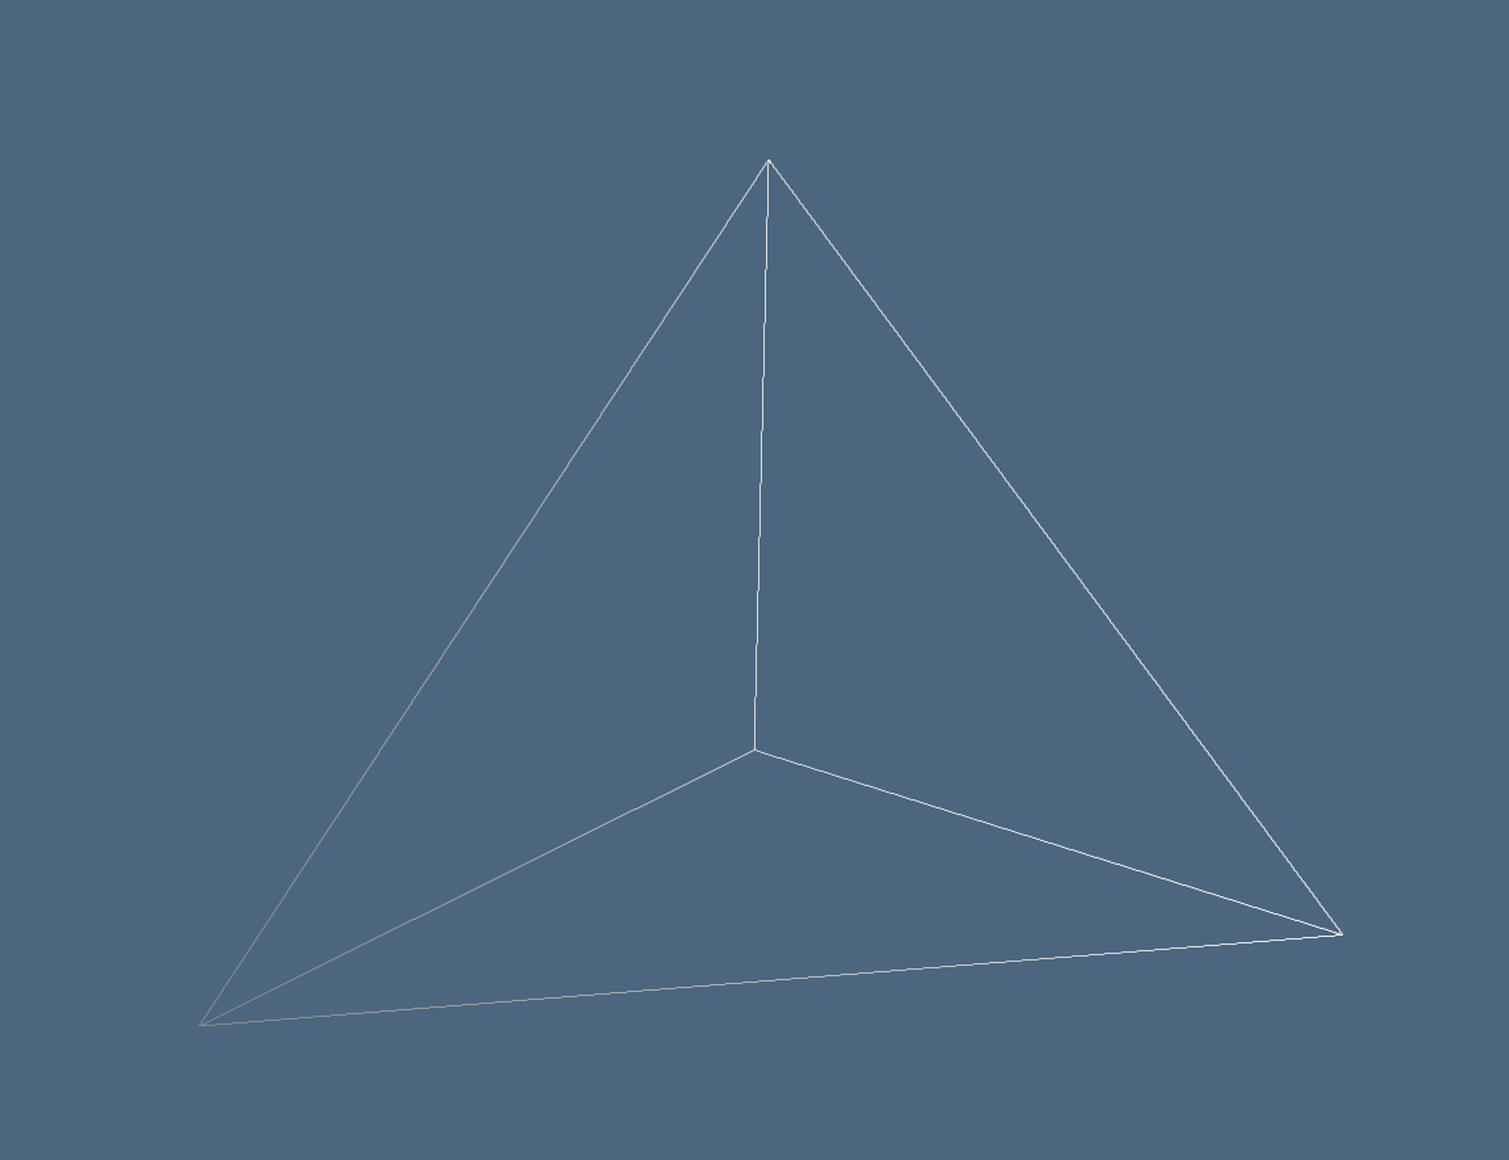
\includegraphics[scale=0.4]{tetra.jpg}

\includegraphics[scale=0.4]{tetra2.jpg}
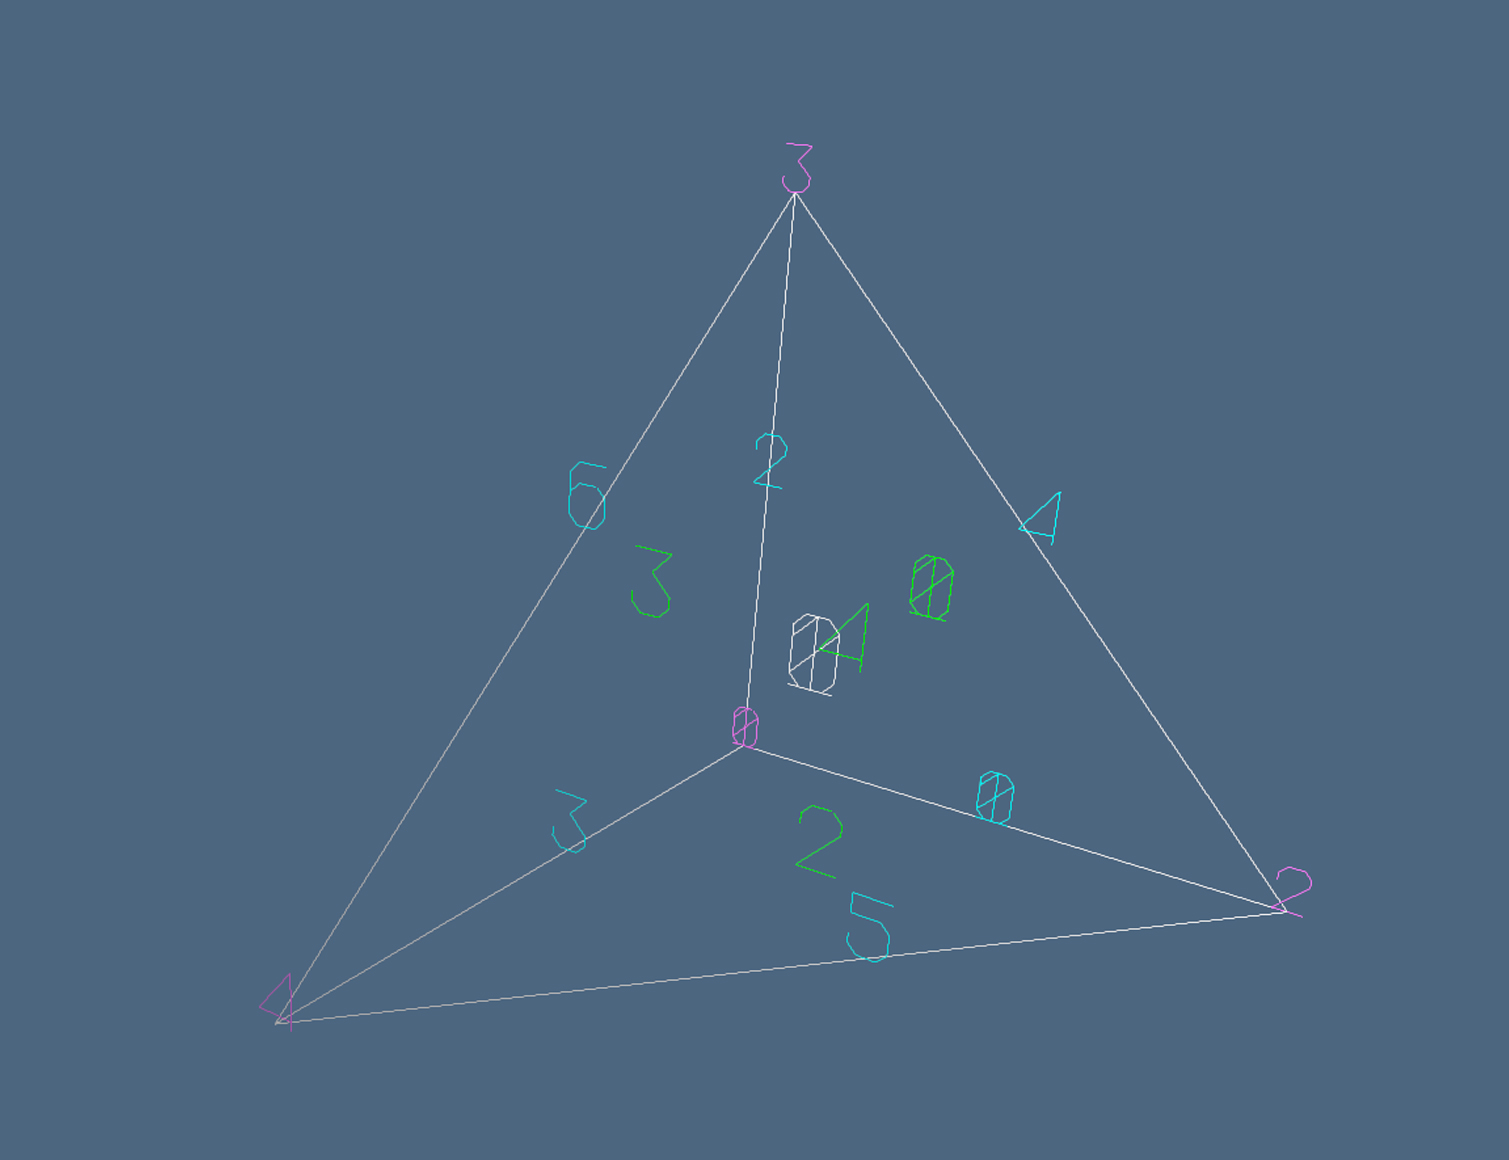
\includegraphics[scale=0.4]{numerazionetetra.jpg}
\caption{Views of  1-, 2-, and 3-dimensional skeletons}
\end{figure}

%-----------------------------------------------------------------
%-----------------------------------------------------------------

\section{Conclusion}
We can conclude that on 4 processes the parallelized module slows down the execution of functions. 
Something could change as the number of processes varies. 

The concept of speedup is aimed at comparing the original serial algorithm with parallel version.
It is calculated:
\[S_p(n)=\frac{t_s(n)}{t_p(n)}\]
where $p$ is number of processes, $n$ is dimension of input, $t_s(n)$ is serial execution time and $t_p(n)$ is parallel execution time.
If $S_p(n) > 1$ then the parallel algorithm is efficient.
\\
\\
We try on Tesla with 40 processes, on different large input, for some functions:
\begin{flushleft}\small
\begin{list}{}{} \item
  \begin{Verbatim}[tabsize=4]
n=40
addprocs(n)

#larCuboidsFacets

input1=larCuboids([5,5,5])
input2=larCuboids([10,10,10])
input3=larCuboids([15,15,15])

times1=@elapsed larCuboidsFacets(input1)
times2=@elapsed larCuboidsFacets(input2)
times3=@elapsed larCuboidsFacets(input3)

timep1=@elapsed pmlarCuboidsFacets(input1)
timep2=@elapsed pmlarCuboidsFacets(input2)
timep3=@elapsed pmlarCuboidsFacets(input3)

y=[times1/timep1,times2/timep2,times3/timep3]

Output: 0.151352
        0.0517906
        0.0313732

#larGridSkeleton

times1=@elapsed larGridSkeleton([5,5,5])(2)
times2=@elapsed larGridSkeleton([10,10,10])(2)
times3=@elapsed larGridSkeleton([15,15,15])(2)

timep1=@elapsed plarGridSkeleton([5,5,5])(2)
timep2=@elapsed plarGridSkeleton([10,10,10])(2)
timep3=@elapsed plarGridSkeleton([15,15,15])(2)

y=[times1/timep1,times2/timep2,times3/timep3]

Output: 0.00191706
        0.00692625
        0.00806735

#larSimplicialStack

times1=@elapsed larSimplicialStack([[1,2,3,4],[2,3,4,5])
times2=@elapsed larSimplicialStack([[1,2,3,4],[2,3,4,5],[3,4,5,6],[4,5,6,7]])
times3=@elapsed larSimplicialStack([[1,2,3,4],[2,3,4,5],[3,4,5,6],[4,5,6,7],[5,6,7,8],[6,7,8,9],[7,8,9,10]])


timep1=@elapsed plarSimplicialStack([[1,2,3,4],[2,3,4,5],[3,4,5,6]])
timep2=@elapsed plarSimplicialStack([[1,2,3,4],[2,3,4,5],[3,4,5,6],[4,5,6,7]])
timep3=@elapsed plarSimplicialStack([[1,2,3,4],[2,3,4,5],[3,4,5,6],[4,5,6,7],[5,6,7,8],[6,7,8,9],[7,8,9,10]])


y=[times1/timep1,times2/timep2,times3/timep3]

Output: 0.0116568
        0.0137202   
        0.00889067
\end{Verbatim}
\end{list}
\end{flushleft}   
\vspace{2ex}
Even though the different ways to parallelized, parallel version is not efficient.  
In general, the vectorized version, for large inputs, helps to speed up on one process.
%-----------------------------------------------------------------

\bibliographystyle{plain}
\bibliography{references}
\end{document}
